\chapter{Auction Theory for Single-Object Auctions}\label{ch:auction-theory}

In most markets the rules of competition are implicit. Auctions are a prominent exception. The seller states how bids
will be turned into an allocation and into payments, and the bidders compete under those rules. Offshore oil leases, timber,
construction contracts, art and online advertising are all sold or bought this way. For empirical industrial
organization the written rules are a gift. In \cref{ch:conduct} the way firms compete was an unknown parameter,
and in \cref{ch:diffprod,ch:blp} marginal costs were recovered only after a demand system had been estimated.
In an auction the game form is known, and the remaining assumptions concern the bidders' information and
equilibrium play. This chapter develops the theory that turns those assumptions into predictions about bids.

The chapter builds the theory of single-object auctions from the ground up. It proves the results that the
book relies on, or sketches the proof where the full argument is long. It starts with the standard formats, the ways in which bidders' information can be related, and
the second-price and ascending auctions, where bidding one's value is a dominant strategy. It then solves the
first-price auction with symmetric independent private values in two ways, proves the revenue equivalence
theorem and derives the optimal auction. A deep dive into \citet{MilgromWeber1982} follows. Their model of
affiliated values explains the winner's curse, the linkage principle, the revenue ranking of the formats and
the seller's incentive to disclose information. The last part relaxes symmetry, fixed participation and
noncooperative bidding, and it treats procurement auctions as the mirror image of sales. Along the way we
report the empirical magnitudes that the survey of \citet{HortacsuPerrigne2021} and the book on bidding rings
by \citet{MarshallMarx2012} attach to the theory. Worked examples with
uniform values run through the chapter. Every number in them is derived in the text or computed numerically
by a method that the text describes.

The chapter is the theoretical half of a pair. Its first-order conditions, which express each value as a bid
plus a markdown, are the equations that \cref{ch:auction-empirics} inverts to recover value distributions from
bid data. The markdown is the buyer's version of the Lerner rule of \cref{ch:theory}, and the inversion mirrors
the recovery of marginal costs in \cref{ch:diffprod}. The analysis of bidding rings connects to the cartel
theory of \cref{ch:collusion-theory} and to the stamp-auction ring of \cref{ch:collusion-evidence}. A merger of
bidders is a special case of the merger analysis of \cref{ch:mergers}. \Cref{app:math} collects the
mathematical tools used here, including the envelope theorem, order statistics and affiliation.
\Cref{sec:14-notation} gives a detailed plan of the chapter and its notation.

\definecolor{c14blue}{HTML}{2A78D6}
\definecolor{c14orange}{HTML}{EB6834}
\definecolor{c14aqua}{HTML}{1BAF7A}
\definecolor{c14gray}{HTML}{52514E}

\section{Why Study Auctions}\label{sec:14-why}

An \emph{auction} is a market institution in which explicit rules map the bids of the participants into an
allocation of the object for sale and a set of payments. Auctions organize a large volume of trade. Art and
antiques, government procurement contracts, offshore oil and gas leases, timber, electricity, Treasury bills
and goods on internet platforms such as eBay are all sold or bought by auction. Internet advertising is
priced by auction as well. Writing in the early 1980s, \citet[p.~1089]{MilgromWeber1982} observed that the
U.S.\ Treasury sold billions of dollars of bills and notes every week by sealed bid. The Department of the
Interior sold mineral rights on federal property at auction. The sums at stake can be large. On September
30, 1980, U.S.\ oil companies paid \$2.8 billion for drilling rights on 147 tracts in the Gulf of Mexico.
The three most expensive tracts sold for \$165 million, \$162 million and \$121 million
\citep[p.~1089, footnote~3]{MilgromWeber1982}.

Auctions are also old. \citet[p.~1089]{MilgromWeber1982}, drawing on \citet{Cassady1967}, recall that the
Greek historian Herodotus described the sale of women as wives in Babylonia around the fifth century B.C.
The auction of plundered booty was common during the closing years of the Roman Empire. In China, the
personal belongings of deceased Buddhist monks were sold at auction as early as the seventh century A.D.

Sellers choose auctions for two practical reasons. The first is \emph{transparency}. A public agency that
procures a road or sells a timber tract under announced rules, with the award determined by the bids,
leaves little room for favoritism. The second is \emph{price discovery}. The seller need not know what the
object is worth, because competition among bidders who know more than the seller pushes the price toward
their valuations.

\subsection{Why auctions are attractive to empirical economists}\label{sec:14-why-data}

The empirical analysis of auction data has grown fast over the past thirty years.
\citet[Section~1, pp.~83--84]{HortacsuPerrigne2021} give three reasons. The first is the volume of trade. A
large share of the goods and services in modern economies is sold or allocated by auction, from
procurement contracts and government securities to spectrum rights and wholesale electricity. With the
internet, auctions have also become the central mechanism for placing advertisements on users' screens.
The second reason is that behavior under well-defined rules is captured well by models of private
information and strategic behavior. Auction theory is among the most successful applications of
microeconomic theory. Six Nobel laureates in economics since 2001 have published on auctions, including
Paul Milgrom and Robert Wilson in 2020 \citep[p.~83]{HortacsuPerrigne2021}.

The third reason is the data. Auction data are plentiful and often public, because transparency laws
require the public agencies that run many auctions to release them. They are also of high quality. The
analyst usually knows the auction mechanism in detail, and the records do not suffer from the
non-response or incomplete response of surveys \citep[pp.~83--84]{HortacsuPerrigne2021}. This matters in
industrial organization, where firms rarely reveal the sensitive information that a researcher needs.
Theory and data also complement each other. Auction theory does not always settle policy questions. For
example, it does not tell a central bank whether to sell Treasury bills by a discriminatory or a uniform
price auction. Empirical work fills such gaps with counterfactuals that predict how revenue or
procurement costs would change under other rules \citep[p.~83]{HortacsuPerrigne2021}.

Two features of auction data make them valuable for structural work. The first is that the data are
rich. Auction records typically contain every bid or at least the winning bid, the identities of the
bidders and of the winner, the number of bidders and characteristics of the object. Many similar objects
are often sold under the same rules, which yields large samples of comparable games.

The second feature is that the rules of the game are known to the researcher. \citet[Section~1]{AtheyHaile2007}
note that the primitives of any strategic model are the set of players, the information structure, the
rules of play and the players' objectives. In auction markets these elements can often be described with
an unusually high degree of confidence. Contrast this with the industries studied in \cref{ch:conduct}.
There the econometrician does not observe whether firms set prices, set quantities or collude, so conduct
becomes a parameter to be estimated. In an auction the seller writes down the game form. The remaining
assumptions concern the bidders' information and equilibrium play.

The structural approach to auctions exploits this feature. A model specifies the joint distribution of the
bidders' values and information, which we call the \emph{primitives}. Equilibrium play maps the primitives
into a distribution of bids. Because the rules are known, this mapping can often be inverted, so that the
observed bids reveal the distribution of private information that generated them. \Cref{ch:auction-empirics}
develops this logic in detail, with formal definitions of identification and testability taken from
\citet[Section~1]{AtheyHaile2007}. Much of what can be learned this way requires no parametric assumptions
on distribution functions. Identification often rests only on restrictions implied by economic theory. The
same authors also stress the limits. Models with common values, risk aversion or unobserved auction
heterogeneity are identified only under strong a priori restrictions, and the difficulty is greatest for
ascending auctions \citep[Section~1]{AtheyHaile2007}.

Structural empirical work on auctions has addressed a wide range of economic questions.
\citet[Section~1]{AtheyHaile2007} list the following, among others.
\begin{itemize}
  \item How are rents divided in auctions of public resources?
  \item Are the reserve prices set in government auctions adequate?
  \item How do mergers of bidders affect procurement costs?
  \item Would different auction rules raise more revenue?
  \item Is the bundling of procurement contracts efficient?
  \item How valuable are seller reputations?
  \item How do the costs of acquiring information affect participation and profits?
  \item Does bidders' private information create adverse selection?
  \item Do bidders behave as if they were risk averse?
\end{itemize}
Auction data also allow us to study the entry of bidders, collusion among bidders and the choice of auction
rules. These questions recur throughout this chapter and \cref{ch:auction-empirics}.

\subsection{A first look at auction data: offshore oil leases}\label{sec:14-why-hp}

\citet{HendricksPorter1988} provide a vivid illustration of how information shapes auction outcomes. The
U.S.\ federal government leased tracts on the Outer Continental Shelf (OCS) off the coasts of Louisiana and
Texas. The leases they study were sold by first-price sealed-bid auctions. The winning bid, called the \emph{bonus},
was paid at the time of the sale. The government also received a royalty equal to one-sixth of the
revenues from any oil or gas extracted \citep[p.~871]{HendricksPorter1988}. If no exploratory work was done
within five years, ownership of the lease reverted to the government. Until the lease expired or production
began, the firm paid a nominal annual rental of \$3 per acre on wildcat tracts and \$10 per acre on drainage
tracts. The government also acted as a bidder in two ways. It announced a reserve price of \$25 per acre on
most drainage leases, and it kept the right to reject the high bid if it judged the bid too low. In the
sample of \citet[p.~871]{HendricksPorter1988}, the high bid was rejected on 7 percent of the wildcat tracts
and on 15 percent of the drainage tracts. Their 144 drainage tracts exclude 25 tracts on which the high bid
was rejected, for which they have no data. \citet[Section~4.1, p.~124]{HortacsuPerrigne2021} describe the
same institutions as typical of these sales.

Two kinds of tracts were sold. A \emph{wildcat} tract lies in an area that has not been drilled, and firms
may acquire only seismic information about it. A \emph{drainage} tract is adjacent to a tract on which a
deposit has been discovered. Firms that own the neighboring tracts learn about the drainage tract from
their own drilling. Other firms rely on private seismic surveys and on observable production from adjacent
tracts \citep[pp.~865--866]{HendricksPorter1988}. \Cref{tab:14-hp-table1} reproduces Table~1 of
\citet{HendricksPorter1988}, which summarizes the wildcat and drainage tracts sold between 1954 and 1969.
Tract value is the estimated ex post present value of revenues minus drilling costs. Net profit is tract
value minus the discounted royalty and bonus payments of the winning firm.

\begin{table}[htbp]
\centering
\caption{Wildcat and drainage tracts on the Outer Continental Shelf, 1954--1969}\label{tab:14-hp-table1}
\begin{tabular}{@{}lcc@{}}
\toprule
 & Wildcat & Drainage \\
\midrule
Number of tracts & 1056 & 144 \\
Number of tracts drilled & 748 & 124 \\
Number of productive tracts & 385 & 86 \\
Average winning bid & 2.67 & 5.76 \\
 & (0.18) & (1.07) \\
Average net profits & 1.22 & 4.63 \\
 & (0.50) & (1.59) \\
Average tract value & 5.27 & 13.51 \\
 & (0.64) & (2.84) \\
Average number of bidders & 3.46 & 2.73 \\
\bottomrule
\end{tabular}

\smallskip
\begin{minipage}{0.8\textwidth}
\footnotesize Notes: Reproduced from \citet[Table~1]{HendricksPorter1988}, who take the figures from
\citet{HendricksPorterBoudreau1987}. Dollar figures are in millions of 1972 dollars. Numbers in parentheses
are standard deviations of the sample means.
\end{minipage}
\end{table}

Several facts stand out \citep[p.~866]{HendricksPorter1988}. Drainage tracts were drilled and found
productive far more often than wildcat tracts. From the table, 86 percent of drainage tracts were drilled
against 71 percent of wildcat tracts, and 60 percent were productive against 36 percent. The average value
of a drainage tract was more than twice that of a wildcat tract. Yet drainage tracts attracted fewer
bidders, 2.73 against 3.46 on average. Average net profit was roughly four times higher on drainage tracts.
The government captured 77 percent of the value of wildcat tracts but only 66 percent of the value of
drainage tracts.

Why would firms compete less for tracts that were more valuable and less risky? The answer lies in the
distribution of information. In a wildcat sale, information is roughly symmetric, because the precision of
seismic surveys is unlikely to vary much across firms. In a drainage sale, the neighbor firms are better
informed. A non-neighbor firm tends to win precisely when the neighbors' information says the tract is
poor. This is a severe form of the \emph{winner's curse}, which \cref{sec:14-winners-curse} studies.
\citet[p.~866]{HendricksPorter1988} report that the neighbor firms' average share of the value of drainage
tracts was about 44 percent, while non-neighbor firms earned approximately zero profits. The example
carries three lessons for this chapter. Values can have a large common component, information can be
distributed asymmetrically, and data on bids and outcomes allow us to test the theory.
\Cref{sec:14-mw-inferior} derives the equilibrium of a first-price auction with one informed bidder, and
\cref{ch:auction-empirics} examines the evidence.

\subsection{Plan of the chapter and notation}\label{sec:14-notation}

The chapter develops the theory in the order in which empirical work uses it. \Cref{sec:14-formats} defines
the standard auction formats and shows which of them are strategically equivalent. \Cref{sec:14-info} sets
out the general model of values and information. It defines affiliation, explains the winner's curse and
collects the facts about order statistics that we use repeatedly. \Cref{sec:14-spa} solves the
second-price and ascending auctions with private values. \Cref{sec:14-fpa} solves the first-price auction
with symmetric independent private values, \cref{sec:14-ret} proves revenue equivalence, and
\cref{sec:14-optimal} characterizes reserve prices and optimal auctions. \Cref{sec:14-mw-eq,sec:14-mw-rank}
study affiliated values following \citet{MilgromWeber1982}. \Cref{sec:14-asym,sec:14-entry,sec:14-collusion}
treat asymmetric bidders, entry and collusion. \Cref{sec:14-procurement} turns to procurement, and
\cref{sec:14-bridge} summarizes what the theory hands to empirical work.

\Cref{tab:14-notation} lists the notation of the chapter. Upper-case letters denote random variables and
lower-case letters their realizations. Bold letters denote vectors. Values and equilibrium bids have
continuous distributions, so ties occur with probability zero and the tie-breaking rule does not matter.
The exceptions are the one-informed-bidder model of \cref{sec:14-mw-inferior} and the weak cartel of
\cref{sec:14-collusion}. There bids have atoms, and ties at the reserve price are broken at random.

\begin{table}[htbp]
\centering
\caption{Notation for the auction chapters}\label{tab:14-notation}
\small
\begin{tabularx}{\textwidth}{@{}p{3.6cm}X@{}}
\toprule
Symbol & Meaning \\
\midrule
$n$, $\mathcal{N}=\{1,\dots,n\}$ & number and set of participating bidders \\
$N$ & number of potential bidders (entry models only) \\
$V_i$, $v_i$ & bidder $i$'s value for the object (random variable, realization) \\
$S_i$, $s_i$, $\bm S$, $\bm S_{-i}$ & bidder $i$'s signal (type), the vector of all signals and the signals of $i$'s rivals \\
$\bm A=(A_1,\dots,A_m)$ & other variables that affect values (object attributes) \\
$S_0$ & the seller's information \\
$u(\bm A,S_i,\bm S_{-i})$ & value function in the general model, $V_i=u(\bm A,S_i,\bm S_{-i})$ \\
$V$ & pure common value \\
$Y_1\ge Y_2\ge\dots\ge Y_{n-1}$ & rivals' signals (or values) in decreasing order, $Y_1=\max_{j\neq i}S_j$ \\
$v(s,y)$ & $\E[V_1\mid S_1=s,Y_1=y]$, expected value given own and highest rival signal \\
$V_{(k:n)}$, $F_{(k:n)}$ & $k$-th lowest of $n$ draws and its CDF \\
$\Lambda_n(x)$ & $nx^{n-1}(1-x)+x^n$, the map from $F$ to the CDF of $V_{(n-1:n)}$ \\
$F$, $f$, $F_i$, $f_i$ & value distribution and density, and their bidder-specific versions \\
$\underline v$, $\bar v$ & lower and upper bounds of the support of values \\
$r$ & reserve price \\
$B_i$, $b_i$, $\beta(\cdot)$, $\beta_i(\cdot)$ & bid and equilibrium bid function \\
$G$, $g$ & CDF and density of one rival's equilibrium bid \\
$M_i=\max_{j\neq i}B_j$ & highest rival bid \\
$P$, $R$ & transaction price and expected revenue $R=\E[P]$ \\
$\phi_i=\beta_i^{-1}$ & inverse bid function of bidder $i$ \\
$G_{M\mid B}$, $g_{M\mid B}$ & distribution and density of the highest rival bid given one's own bid \\
$L(\alpha\mid s)$ & integrating factor of the first-price equilibrium with affiliated signals \\
$q_i(\bm v)$, $\tau_i(\bm v)$ & allocation and payment rules of a direct mechanism \\
$Q_i(v)$, $m_i(v)$, $\pi_i(v)$ & interim probability of winning, expected payment and expected surplus \\
$\psi_i(v)$ & virtual valuation $v-\frac{1-F_i(v)}{f_i(v)}$ \\
$v_0$ & seller's own value for the object (not a reserve price) \\
$\eta(b)$ & elasticity of the probability of winning with respect to the bid \\
$\mathcal{U}$ & bidder's utility of money, with $\mathcal{U}(0)=0$ \\
$K$, $p$ & entry cost and entry probability (entry models only) \\
$\pi(k)$, $\Pi(p)$ & expected profit of an entrant facing $k-1$ rivals, ex ante profit from entry \\
$\omega$ & half-width of the uniform noise in the mineral rights example \\
$c_i$, $F_c$ & costs and their distribution in procurement auctions \\
\bottomrule
\end{tabularx}
\end{table}

\section{Auction Formats and Strategic Equivalence}\label{sec:14-formats}

Auctions differ in many details. Three questions classify the formats used in practice. How many objects
are sold? How do the allocation and the payments depend on the bids? How is the bidding organized? This
section answers them, defines the formats we study and shows that some formats that look different are the
same game.

\subsection{A classification}\label{sec:14-formats-class}

The first question is the number of objects. In a \emph{single-unit} auction one indivisible object is sold
or procured, such as an oil lease, a painting, a road construction contract or a timber tract. In a
\emph{multi-unit} auction many units are sold at once, as in auctions of Treasury bills, electricity and
spectrum licenses. Multi-unit auctions use either \emph{discriminatory} (pay-as-bid) pricing, in which each
winning bid pays its own price, or \emph{uniform} pricing, in which all winning units pay one
market-clearing price. This book treats single-unit auctions, apart from a short treatment of
divisible-good auctions in \cref{sec:15-divisible}.

The second question is the rule that determines the winner and the payments. In a \emph{first-price}
auction the highest bidder wins and pays its own bid. First-price rules govern most public procurement and
some timber sales. In a \emph{second-price} auction the highest bidder wins and pays the second-highest bid.
Second-price payment rules, or rules that produce the same outcome, are used in internet advertising, on
eBay and in art sales.

The third question is how bids are submitted. In a \emph{sealed-bid} auction each bidder submits one bid
without observing the others. Procurement auctions, Treasury bill auctions, internet advertising and some
timber sales use sealed bids. In an \emph{open ascending} auction the price rises until only one bidder
remains. Art sales, eBay and some timber sales are open ascending auctions. In an \emph{open descending}
auction the price falls until a bidder accepts it. Flowers for export are sold this way in the
Netherlands \citep[footnote~5]{MilgromWeber1982}, and so are some corporate debt securities and initial
public offerings.

Combining the answers gives the four standard single-object formats. We define them formally for $n$
bidders and a reserve price $r\ge 0$.

\begin{definition}[Standard single-object auctions]\label{def:14-formats}
A \emph{reserve price} $r$ is the minimum bid the seller accepts. Bids below $r$ are rejected, which is the
same as not participating.
\begin{enumerate}[label=(\roman*)]
  \item In the \emph{first-price sealed-bid auction} (FPA) bidders submit bids simultaneously. The highest
  bid wins if it is at least $r$, and the winner pays its bid.
  \item In the \emph{second-price sealed-bid auction} (SPA, or \emph{Vickrey auction}) bidders submit bids
  simultaneously. The highest bid wins if it is at least $r$, and the winner pays the larger of $r$ and the
  highest rival bid.
  \item In the \emph{English auction} the price rises continuously and bidders drop out until one bidder
  remains, who wins at the price at which the last rival dropped out. \Cref{def:14-button} makes the rules
  precise.
  \item In the \emph{Dutch auction} the auctioneer starts at a price above any bidder's value and lowers it
  continuously. The first bidder to stop the clock wins and pays the current price, provided it is at
  least $r$.
\end{enumerate}
\end{definition}

With private values and risk neutrality, bidder $i$'s payoffs in the two sealed-bid formats are
\begin{align}
u_i^{\mathrm{FP}} &= (v_i-b_i)\,\indic\Bigl\{b_i>\max_{j\neq i}b_j,\ b_i\ge r\Bigr\}, \label{eq:14-payoff-fpa}\\
u_i^{\mathrm{SP}} &= \Bigl(v_i-\max\bigl\{r,\max_{j\neq i}b_j\bigr\}\Bigr)\,\indic\Bigl\{b_i>\max_{j\neq i}b_j,\ b_i\ge r\Bigr\}.
\label{eq:14-payoff-spa}
\end{align}
Two further formats are useful as theoretical devices. In an \emph{all-pay auction} every bidder pays its
bid and the highest bid wins. In a \emph{third-price auction} with $n\ge 3$ bidders the highest bid wins
and pays the third-highest bid. \Cref{sec:14-ret} uses both to illustrate revenue equivalence.

An \emph{entry fee} is a payment required to submit a bid. Reserve prices and entry fees both screen out
bidders with low values, and \cref{sec:14-optimal} studies the resulting trade-off. In a \emph{procurement}
(or low-bid) auction a buyer purchases a contract and the bidders are sellers. Each seller has a cost $c_i$,
the lowest bid wins, and the reserve price is the highest price the buyer accepts. Every result in this
chapter has a mirror image for procurement, with costs in place of values and the inequalities reversed.
\Cref{sec:14-procurement} spells this out. \Cref{tab:14-formats} summarizes the formats.

\begin{table}[htbp]
\centering
\caption{Standard single-object auction formats}\label{tab:14-formats}
\small
\begin{tabularx}{\textwidth}{@{}>{\raggedright\arraybackslash}p{2.35cm}>{\raggedright\arraybackslash}p{2.0cm}>{\raggedright\arraybackslash}p{2.45cm}>{\raggedright\arraybackslash}X>{\raggedright\arraybackslash}X@{}}
\toprule
Format & Winner & Winner pays & Information revealed during the auction & Typical uses \\
\midrule
First-price sealed-bid & highest bid & own bid & none & public procurement, offshore oil and gas
leases, some timber sales \\
\addlinespace
Second-price sealed-bid (Vickrey) & highest bid & highest rival bid & none & rare in pure form (internet
advertising and eBay proxy bidding use related rules) \\
\addlinespace
English (ascending, button model) & last active bidder & price at which the last rival quits & exit prices
and number of active bidders & art and antiques, timber, internet auctions \\
\addlinespace
Dutch (descending) & first bidder to stop the clock & price on the clock & none before the auction ends &
flowers in the Netherlands, some debt securities and IPOs \\
\addlinespace
Procurement (low-bid) & lowest bid & own bid, or the lowest rival bid in second-price versions & as in the
corresponding sale format & construction and highway contracts, government purchases \\
\bottomrule
\end{tabularx}

\smallskip
\begin{minipage}{\textwidth}
\footnotesize Notes: With a reserve price $r$, bids below $r$ are rejected and a winner pays at least $r$
(at most $r$ in procurement). Uses follow \citet[pp.~1089--1091]{MilgromWeber1982},
\citet[Section~1 and footnote~2]{AtheyHaile2007}, \citet[p.~871]{HendricksPorter1988} and
\citet[pp.~86, 101 and 124]{HortacsuPerrigne2021}.
\end{minipage}
\end{table}

The institutions vary with the good for sale, and \citet{HortacsuPerrigne2021} organize their survey of
empirical work around this fact. Governments sell timber harvesting contracts by both first-price
sealed bids and ascending auctions, often with binding reserve prices. In U.S.\ Forest Service
\emph{scale auctions}, a bidder submits a price per unit of each species on the tract. The agency ranks
bids by their inner product with its own estimates of species volumes. The winner then pays on the
volumes harvested. Bidders usually survey the tract themselves before bidding, a step called a
\emph{cruise} \citep[Section~2, p.~86]{HortacsuPerrigne2021}. Most procurement auctions are first-price
sealed-bid. Contractors bid unit prices on a list of line items with estimated quantities, and public
procurement alone accounts for an estimated 10 percent of U.S.\ GDP \citep[Section~3,
p.~101]{HortacsuPerrigne2021}. Oil and gas leases are usually sold by first-price sealed bid
\citep[Section~4, p.~124]{HortacsuPerrigne2021}.

\subsection{Varieties of the English auction}\label{sec:14-formats-english}

The English auction comes in several variants, and they are different games
\citep[pp.~1103--1104]{MilgromWeber1982}. In some, the bidders call out their own bids and the auction
ends when nobody is willing to raise the standing bid. In others, the auctioneer calls the bids and a
willing bidder indicates assent by a slight gesture, often in a way that preserves the bidder's anonymity.
In a variant used in Japan and described by \citet{Cassady1967}, the price is posted on an electronic
display and rises continuously. A bidder who wishes to remain active holds down a button. Releasing the
button is an irreversible withdrawal.

\begin{definition}[Button auction]\label{def:14-button}
Following \citet[p.~1104]{MilgromWeber1982} and \citet[Section~2.2.2]{AtheyHaile2007}, the \emph{button
auction} (or \emph{clock auction}) has the following rules.
\begin{enumerate}[label=(\roman*)]
  \item All bidders are active at the starting price, which is zero or the reserve price $r$.
  \item The price $p$ rises continuously.
  \item A bidder may drop out at any price, and a bidder who has dropped out cannot become active again.
  \item The price at which each bidder drops out and the number of active bidders are observed by all.
  \item When one bidder remains, the auction ends. That bidder obtains the object and pays the price at
  which the last rival dropped out.
\end{enumerate}
\end{definition}

From now on, the term English auction refers to the button auction. A strategy specifies the price at which
to quit as a function of the bidder's signal and of the exits observed so far. If $k$ rivals have quit at
prices $p_1\le\dots\le p_k$, bidder $i$'s strategy is a function $\beta_{ik}(s_i\mid p_1,\dots,p_k)\ge p_k$.
It gives the price at which $i$ quits if no further exit occurs first \citep[p.~1104]{MilgromWeber1982}.
The auction ends at the second-highest exit price. \Cref{fig:14-button} illustrates a button auction with
four bidders who quit at their values.

\begin{figure}[htbp]
\centering
\begin{tikzpicture}[x=1.25cm,y=1.25cm,>=Stealth]
  \draw[->] (0,0) -- (7.6,0) node[below left] {time};
  \draw[->] (0,0) -- (0,4.4) node[above] {price $p$};
  \foreach \y/\lab in {1.2/{(1:4)},2.0/{(2:4)},2.9/{(3:4)},3.8/{(4:4)}} {
    \draw[densely dashed,c14gray!60] (0,\y) -- (6.9,\y) node[right,black] {$v_{\lab}$};
  }
  \draw[very thick,c14blue] (0,0) -- (2.9,2.9);
  \draw[thick,dotted,c14blue] (2.9,2.9) -- (3.8,3.8);
  \foreach \y in {1.2,2.0,2.9} { \fill[c14orange] (\y,\y) circle (2.2pt); }
  \node[font=\footnotesize,anchor=north west] at (0.60,0.50) {4 active};
  \node[font=\footnotesize,anchor=north west] at (1.45,1.15) {3 active};
  \node[font=\footnotesize,anchor=north west] at (2.25,1.95) {2 active};
  \node[font=\footnotesize,align=left,anchor=west] at (3.35,2.45) {auction ends: the remaining bidder\\ wins and pays $v_{(3:4)}$};
  \draw[->,c14gray] (3.33,2.55) -- (3.0,2.85);
  \node[font=\footnotesize,align=right,anchor=east] at (2.95,3.36) {price at which the\\ winner would have quit};
  \draw[->,c14gray] (3.0,3.45) -- (3.72,3.76);
\end{tikzpicture}
\caption{A button auction with four bidders. The price rises continuously. Each bidder quits when the price
reaches its value (dots), and the number of active bidders is public. The auction ends at the
second-highest value $v_{(3:4)}$, and the bidder with the highest value $v_{(4:4)}$ wins.}
\label{fig:14-button}
\end{figure}

Real open-outcry auctions depart from this idealization. Bidders call their own prices and may raise the
standing bid by large jumps. A bidder may stay silent until late in the auction and need not reveal the
price at which it would quit. \citet[Section~2.2.2]{AtheyHaile2007} warn that the button model may then be
too great an abstraction. \citet{HaileTamer2003} replace it with two weak behavioral restrictions. Bidders
never bid more than they are willing to pay, and they never let a rival win at a price they would have been
willing to beat. \Cref{ch:auction-empirics} shows that these restrictions yield bounds on the distribution
of values.

\subsection{Strategic equivalence}\label{sec:14-formats-equiv}

Some formats that look different are the same game. The following definition makes this precise.

\begin{definition}[Strategic equivalence]\label{def:14-strat-equiv}
Two auction formats are \emph{strategically equivalent} if, for every bidder, there is a one-to-one
correspondence between the strategies available in the two formats with the following property. Every
profile of corresponding strategies produces the same allocation and the same payments, for every
realization of the bidders' information.
\end{definition}

Strategic equivalence is a property of the rules alone. Payoffs depend on the rules only through the
allocation and the payments. Strategically equivalent formats therefore give every bidder the same expected
payoff under every strategy profile, so they have the same equilibria. This conclusion holds whatever the
bidders' values, information and attitudes toward risk. The equilibrium concept throughout is
\emph{Bayesian Nash equilibrium}, a profile of strategies in which each bidder's strategy maximizes its
expected payoff given its own information and the strategies of the others. \Cref{def:14-bne} states it
formally.

\begin{proposition}[Dutch and first-price auctions]\label{prop:14-dutch-fpa}
For any number of bidders, any distribution of values and signals and any preferences over outcomes,
the Dutch auction and the first-price sealed-bid auction with the same reserve price are strategically
equivalent. Their sets of Bayesian Nash equilibria coincide, and corresponding equilibria produce the same
allocation and payments.
\end{proposition}

\begin{proof}
Consider the Dutch auction. The game ends at the first moment at which some bidder stops the clock. Before
that moment, the only event a bidder can observe is that nobody has stopped the clock yet. This event is
implied by the fact that the game is still being played. It therefore carries no information beyond the
current price, which every bidder can foresee. The decision of a bidder is essentially static
\citep[p.~1091]{MilgromWeber1982}. A strategy reduces to a function $b_i(s_i)$ that gives the price at which
bidder $i$ will stop the clock if nobody has stopped it earlier, where $b_i(s_i)<r$ means never stopping.
Given a profile $(b_1,\dots,b_n)$, the winner is the bidder with the highest stopping price, provided it is
at least $r$, and the winner pays that price.

In the first-price auction a strategy is a function $b_i(s_i)$ that gives the sealed bid. The winner is the
highest bidder, provided the bid is at least $r$, and the winner pays its bid. Map each Dutch strategy to
the first-price strategy given by the same function $b_i(\cdot)$. This map is one-to-one. Under it, every
profile yields the same winner and the same payment for every realization of the signals. The two formats
are therefore strategically equivalent, and the equality of their equilibria follows.
\end{proof}

\begin{remark}
The argument uses no assumption about values \citep[footnote~11]{MilgromWeber1982}. A bidder need not know
its value, and values may be private or common. What the argument requires is that bidders learn nothing
while the clock falls. This holds because no bidder acts before the game ends.
\end{remark}

\begin{proposition}[English and second-price auctions with two bidders]\label{prop:14-english-spa-n2}
With two bidders, the English (button) auction and the second-price sealed-bid auction with the same
reserve price are strategically equivalent, for any joint distribution of values and signals.
\end{proposition}

\begin{proof}
In the button auction with two bidders, each bidder observes only that its rival is still active as long as
both are active. The first exit ends the auction. A strategy is therefore a single number for each signal,
the price $d_i(s_i)$ up to which bidder $i$ stays in if the rival is still active
\citep[p.~1104]{MilgromWeber1982}. A choice $d_i(s_i)<r$ means not participating. The bidder with the higher
number wins and pays the price at which the rival quits. That price is the rival's number, or $r$ if the
rival does not participate. In the second-price auction the bidder with the higher bid wins and pays the
larger of $r$ and the rival's bid. Map each English strategy $d_i(\cdot)$ to the sealed bid
$b_i(\cdot)=d_i(\cdot)$. The map is one-to-one, and corresponding profiles give identical outcomes for every
realization of the signals.
\end{proof}

\begin{remark}\label{rem:14-english-n3}
With three or more bidders the equivalence fails. The prices at which the first bidders quit are public,
and a remaining bidder can condition its own quitting price on them through the functions $\beta_{ik}$. The
strategy sets of the English auction are therefore strictly richer than those of the second-price auction.
With interdependent values, early exits also convey information about the value of the object
\citep[p.~1104]{MilgromWeber1982}. Under private values the two formats remain equivalent in a weaker sense.
Each has a dominant strategy equilibrium, and the two equilibria produce the same outcome
(\cref{sec:14-spa}). Under affiliated interdependent values the English auction raises at least as
much expected revenue as the second-price auction (\cref{prop:14-mw-ranking}).
\end{remark}

\section{Values, Signals, and Information Structures}\label{sec:14-info}

What a bidder knows, and how that knowledge relates to the value of the object, drives auction theory. It
determines equilibrium bids, the ranking of formats by revenue and what bid data can reveal. This section
sets up a general model and classifies its special cases. It then develops three tools used throughout the
chapter, namely affiliation, the winner's curse and order statistics.

\subsection{The general model}\label{sec:14-info-model}

There are $n\ge 2$ bidders, indexed by $i\in\mathcal{N}=\{1,\dots,n\}$, who compete for a single indivisible
object. Bidder $i$'s \emph{value} $V_i$ is the money value of the object to bidder $i$. It may depend on
variables nobody knows at the time of the auction, such as the amount of oil in a tract or the price at
which a painting can be resold. Bidder $i$'s private information is summarized by a scalar \emph{signal}
$S_i$, also called its \emph{type}, with support $[\underline s_i,\bar s_i]$. We write
$\bm S=(S_1,\dots,S_n)$ for the vector of signals, $\bm S_{-i}$ for the signals of $i$'s rivals and $B_i$
for $i$'s bid. These conventions follow \citet[Section~2.1]{AtheyHaile2007}.

We maintain two assumptions on preferences unless we say otherwise. There are \emph{no externalities}, so a
losing bidder's payoff does not depend on who wins. Bidders are \emph{risk neutral}. A bidder who wins and
pays $P$ receives $V_i-P$, and a bidder who loses and pays nothing receives zero. Bidder $i$'s expected
payoff from winning, gross of the payment and conditional on all signals, is
\begin{equation}\label{eq:14-cond-value}
\E\bigl[V_i\mid S_i=s_i,\bm S_{-i}=\bm s_{-i}\bigr].
\end{equation}

Information is \emph{incomplete}. Bidder $i$ observes the realization $s_i$ of its own signal but not the
rivals' signals. Under \emph{complete information} each bidder would also observe $\bm s_{-i}$. The set of
bidders and the joint distribution $F_{\bm S,\bm V}$ of signals and values are common knowledge
\citep[Section~2.1]{AtheyHaile2007}. Signals are \emph{informative}, in the sense that the expectation
\eqref{eq:14-cond-value} strictly increases in $s_i$ for every $\bm s_{-i}$.

Models of auctions differ along two dimensions. The first is statistical. Signals are \emph{independent} if
their joint distribution is the product of the marginal distributions, $F_{\bm S}=\prod_{i=1}^{n}F_i$, and
\emph{dependent} otherwise. The second dimension concerns whether rivals' information matters for a
bidder's own value.

\begin{definition}[Private and common values]\label{def:14-private-values}
Bidders have \emph{private values} if, for all $i$ and all $\bm s$,
\begin{equation}\label{eq:14-pv-def}
\E\bigl[V_i\mid \bm S=\bm s\bigr]=\E\bigl[V_i\mid S_i=s_i\bigr].
\end{equation}
Bidders have \emph{common values} if, for all $i$ and $j$, $\E[V_i\mid\bm S=\bm s]$ strictly increases in
$s_j$ \citep[Definition~2.1]{AtheyHaile2007}.
\end{definition}

Under private values, a bidder has no private information about its rivals' values. A bidder would like to
know its rivals' signals for strategic reasons, to predict their bids. Learning them would not change its
estimate of its own value. Under common values, learning a rival's signal would change that estimate. This
is the source of the winner's curse \citep[Section~2.1]{AtheyHaile2007}. The two definitions are not
exhaustive. A model in which $V_i$ depends on some rivals' signals but not on others, or only for some
realizations, is neither. \citet[footnote~6]{AtheyHaile2007} adopt the strict definition of common values
for simplicity. Some authors use the term \emph{interdependent values} for the whole framework that allows
both private and common values \citep[footnote~8]{AtheyHaile2007}.

Signals play a purely informational role. Any strictly increasing transformation of $S_i$ contains the same
information as $S_i$ itself, so the marginal distribution of $S_i$ is not a primitive of the model.
Without loss of generality we may therefore impose the normalization
\begin{equation}\label{eq:14-normalization}
S_i=\E\bigl[V_i\mid S_i\bigr].
\end{equation}
\citet[footnote~5]{AtheyHaile2007} stress that this degree of freedom belongs to the theoretical model and
has nothing to do with econometric identification. Under private values, \eqref{eq:14-pv-def} and
\eqref{eq:14-normalization} give $\E[V_i\mid\bm S]=S_i$. A risk-neutral bidder then behaves exactly as if
it knew its value to be $S_i$. In private-values models we therefore set $V_i=S_i$ and speak of bidder
$i$'s value $v_i$.

\begin{remark}[A common factor does not create common values]\label{rem:14-common-factor}
Suppose that
\begin{equation}\label{eq:14-common-factor}
S_i=V_i=V_0+\epsilon_i,\qquad i=1,\dots,n,
\end{equation}
where $V_0$ is a shock common to all bidders and $\epsilon_i$ is idiosyncratic. This is a private-values
model, because each bidder knows its own value with certainty \citep[Section~7]{AtheyHaile2007}. The common
factor $V_0$ makes values and signals correlated across bidders. It even makes one bidder's signal
correlated with another bidder's value. Still, once bidder $i$ has seen $s_i$, no rival has information
relevant to $i$'s value. Private values also allow noise in a bidder's own value. Let $V_i=S_i+\eta_i$, where
the noise $\eta_i$ is independent of the whole signal vector $\bm S$. Then $\E[V_i\mid\bm S]=S_i+\E[\eta_i]$,
which depends on $S_i$ alone. \citet[footnote~78]{AtheyHaile2007} ask only that $\eta_i$ be independent of
each rival signal $S_j$, $j\neq i$. That weaker condition is not enough, because $S_i$ itself can depend on
$\eta_i$. Let $\eta_1$ and $S_2$ be independent and uniform on $[0,1]$, and let $S_1=\eta_1+S_2$. Then
$\E[V_1\mid S_1,S_2]=2S_1-S_2$. By symmetry $\E[\eta_1\mid S_1]=\frac{1}{2}S_1$, so
$\E[V_1\mid S_1]=\frac{3}{2}S_1$ and the rival's signal is informative. The distinction between private
and common values concerns
what rivals know about one's own value. Correlation of values is a separate matter.
\end{remark}

\citet{MilgromWeber1982} proposed a general symmetric model that nests the private and common value
models. Let $\bm A=(A_1,\dots,A_m)$ be a vector of additional real-valued variables that influence the value
of the object to the bidders. Some components of $\bm A$ may be observed by the seller, such as appraisals
of a painting. Others may be observed by nobody at the time of the sale, such as the tastes of
connoisseurs who will determine its resale value \citep[p.~1097]{MilgromWeber1982}. Bidder $i$'s value is
$V_i=u_i(\bm A,\bm S)$, and $f(\bm a,\bm s)$ denotes the joint density of $(\bm A,\bm S)$. Milgrom and
Weber write $S$ for our $\bm A$ and $X$ for our $\bm S$.

\begin{assumption}[General symmetric model]\label{ass:14-mw}
The following hold \citep[Assumptions~1--5, pp.~1097--1098]{MilgromWeber1982}.
\begin{enumerate}[label=(\roman*)]
  \item There is a function $u$ on $\R^{m+n}$ such that $u_i(\bm A,\bm S)=u(\bm A,S_i,\{S_j\}_{j\neq i})$ for
  all $i$. All bidders' values depend on $\bm A$ in the same manner, and each bidder's value is a
  symmetric function of the rivals' signals.
  \item The function $u$ is nonnegative, continuous and nondecreasing in all its arguments.
  \item For each $i$, $\E[V_i]<\infty$.
  \item The density $f$ is symmetric in its last $n$ arguments, the signals.
  \item The variables $A_1,\dots,A_m,S_1,\dots,S_n$ are affiliated (\cref{def:14-affiliation} below).
\end{enumerate}
\end{assumption}

The private-values model is the special case $m=0$ and $V_i=S_i$. The pure common value model is the
special case $m=1$ and $V_i=A_1$ for every $i$ \citep[p.~1098]{MilgromWeber1982}. Bidders are risk neutral,
so a bidder who wins and pays $b$ receives $V_i-b$. \Cref{sec:14-mw-risk} discusses risk aversion in this
model.

Two features of \cref{ass:14-mw} deserve comment. First, summarizing a bidder's information by one real
number is a substantive assumption. The signal must be a sufficient statistic for the bidder's information
about its own value, and it must also summarize what the bidder knows about the rivals' signals
\citep[footnote~14]{MilgromWeber1982}. Second, the existence of a joint density simplifies the statements.
All results except the explicit formulas for equilibrium strategies survive without it, with randomized
strategies in place of pure ones \citep[footnote~15]{MilgromWeber1982}.

\citet[Section~2.3]{MilgromWeber1982} motivate the general model with the sale of a painting. The
independent private values model requires that each bidder know its value and that values be
statistically independent. The first requirement rules out resale at an unknown price, the prestige of
owning a painting that others admire and doubts about authenticity. The second rules out a bidder
inferring from its own admiration of the painting that others are likely to value it highly too. The
general model allows all of these.

\subsection{A taxonomy of information structures}\label{sec:14-info-taxonomy}

Restrictions on the joint distribution of signals and values generate the special cases used in the
literature. Following \citet[Section~2.1]{AtheyHaile2007}, we list the main ones.
\begin{itemize}
  \item \emph{Independent private values} (IPV) are private values with $V_1,\dots,V_n$ independent.
  \item \emph{Symmetric independent private values} (SIPV) are private values with $V_1,\dots,V_n$
  independent and identically distributed with CDF $F$, so that
  $F_{\bm V}(v_1,\dots,v_n)=\prod_{i=1}^{n}F(v_i)$.
  \item \emph{Affiliated private values} (APV) are private values with $(V_1,\dots,V_n)$ affiliated.
  \item Values are \emph{common} (CV) when $\E[V_i\mid\bm S]$ strictly increases in every signal, as in
  \cref{def:14-private-values}.
  \item \emph{Pure common values} are common values with $V_i=V$ for all $i$, so that the object is worth
  the same to every bidder.
  \item The \emph{mineral rights} model has pure common values and signals that are independent and
  identically distributed conditional on $V$ \citep{Wilson1977}.
  \item The \emph{general symmetric model} of \cref{ass:14-mw} nests the symmetric versions of all of the
  above whose signals are affiliated.
\end{itemize}
A model is \emph{symmetric} if the joint distribution of signals and values is exchangeable in the bidder
indices, and \emph{asymmetric} otherwise. Terminology varies across papers. Early work sometimes used
``common values'' for what we call pure common values. It sometimes used ``affiliated values'' for what we
call common values, even though private values can be affiliated \citep[footnote~8]{AtheyHaile2007}.

Dependence of signals is neither necessary nor sufficient for common values
\citep[Section~2.1]{AtheyHaile2007}. Affiliated private values combine dependent signals with private
values. Conversely, let $S_1$ and $S_2$ be independent and uniform on $[0,1]$, and suppose both bidders
value the object at $V=\frac{S_1+S_2}{2}$. Signals are independent, yet each bidder's value rises with the
rival's signal, so values are common. \Cref{ex:14-iv-independent} solves this example. \Cref{fig:14-taxonomy} maps the
models, and \cref{tab:14-info} gives definitions and examples.

\begin{figure}[htbp]
\centering
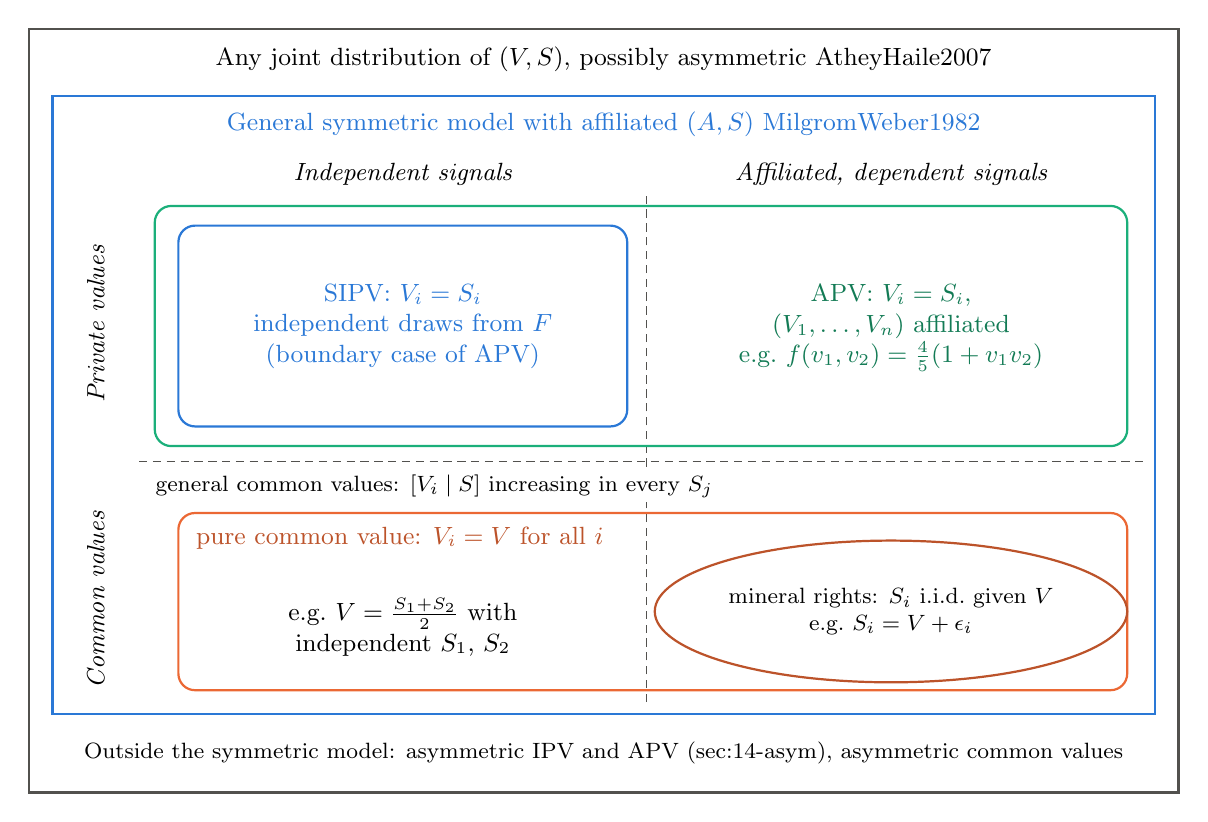
\begin{tikzpicture}[x=1cm,y=1cm,font=\small]
  \draw[thick,c14gray] (0,0) rectangle (14.6,9.7);
  \node[align=center,anchor=north] at (7.3,9.6) {Any joint distribution of $(\bm V,\bm S)$, possibly
  asymmetric \citep{AtheyHaile2007}};
  \draw[thick,c14blue] (0.3,1.0) rectangle (14.3,8.85);
  \node[align=center,anchor=north,c14blue,text width=13.4cm] at (7.3,8.77) {General symmetric model with
  affiliated $(\bm A,\bm S)$ \citep{MilgromWeber1982}};
  \node[align=center,font=\small\itshape] at (4.75,7.85) {Independent signals};
  \node[align=center,font=\small\itshape] at (10.95,7.85) {Affiliated, dependent signals};
  \node[rotate=90,font=\small\itshape] at (0.85,5.95) {Private values};
  \node[rotate=90,font=\small\itshape] at (0.85,2.45) {Common values};
  \draw[densely dashed,c14gray] (7.85,1.15) -- (7.85,7.6);
  \draw[densely dashed,c14gray] (1.4,4.2) -- (14.15,4.2);
  \draw[rounded corners=6pt,thick,c14aqua] (1.6,4.4) rectangle (13.95,7.45);
  \node[align=center,c14aqua!70!black] at (10.95,5.9) {APV: $V_i=S_i$,\\ $(V_1,\dots,V_n)$ affiliated\\
  e.g.\ $f(v_1,v_2)=\frac{4}{5}(1+v_1v_2)$};
  \draw[rounded corners=6pt,thick,c14blue] (1.9,4.65) rectangle (7.6,7.2);
  \node[align=center,c14blue] at (4.75,5.92) {SIPV: $V_i=S_i$\\ independent draws from $F$\\ (boundary case of
  APV)};
  \node[align=left,anchor=north west,font=\footnotesize,fill=white,inner sep=1.5pt] at (1.55,4.1) {general
  common values: $\E[V_i\mid\bm S]$ increasing in every $S_j$};
  \draw[rounded corners=6pt,thick,c14orange] (1.9,1.3) rectangle (13.95,3.55);
  \node[align=left,anchor=north west,c14orange!80!black] at (2.0,3.5) {pure common value: $V_i=V$ for all $i$};
  \node[align=center] at (4.75,2.1) {e.g.\ $V=\frac{S_1+S_2}{2}$ with\\ independent $S_1$, $S_2$};
  \draw[thick,c14orange!80!black] (10.95,2.3) ellipse (3.0 and 0.9);
  \node[align=center,font=\footnotesize] at (10.95,2.3) {mineral rights: $S_i$ i.i.d.\ given $V$\\ e.g.\
  $S_i=V+\epsilon_i$};
  \node[align=center,font=\footnotesize] at (7.3,0.5) {Outside the symmetric model: asymmetric IPV and APV
  (\cref{sec:14-asym}), asymmetric common values};
\end{tikzpicture}
\caption{A map of information structures. Columns separate independent from affiliated signals, and rows
separate private from common values. Independence is the boundary case of affiliation, so SIPV lies inside
APV. Pure common values can have independent or dependent signals. The mineral rights model has dependent
signals. All symmetric models with affiliated signals and values are special cases of the general model of
\citet{MilgromWeber1982}.}
\label{fig:14-taxonomy}
\end{figure}

\begin{table}[htbp]
\centering
\caption{Information structures: definitions and canonical examples}\label{tab:14-info}
\small
\begin{tabularx}{\textwidth}{@{}>{\raggedright\arraybackslash}p{2.9cm}>{\raggedright\arraybackslash}X>{\raggedright\arraybackslash}X@{}}
\toprule
Model & Definition & Example \\
\midrule
SIPV & $V_i=S_i$, values i.i.d.\ with CDF $F$ & nondurable consumer goods bought for own use
\citep[p.~1093]{MilgromWeber1982} \\
\addlinespace
IPV (asymmetric) & $V_i=S_i$, values independent with CDFs $F_i$ & timber tracts sold to mills and loggers with
different costs \citep{AtheyLevinSeira2011} \\
\addlinespace
APV & $V_i=S_i$, $(V_1,\dots,V_n)$ affiliated & a painting bought for own enjoyment by bidders with correlated
tastes \citep[p.~1099]{MilgromWeber1982} \\
\addlinespace
Common values & $\E[V_i\mid\bm S]$ strictly increasing in every $S_j$ & timber: private cost differences
plus private estimates of timber quality, volume and future market conditions
\citep[Section~II.F]{AtheyLevinSeira2011} \\
\addlinespace
Pure common value & $V_i=V$ for all $i$ & oil, gas and mineral rights \citep[Section~2.2]{MilgromWeber1982} \\
\addlinespace
Mineral rights & pure common value, $S_i$ i.i.d.\ given $V$ & offshore oil tract with independent seismic
estimates \citep[p.~1094]{MilgromWeber1982} \\
\addlinespace
General symmetric model & $V_i=u(\bm A,S_i,\bm S_{-i})$, $u$ symmetric, $(\bm A,\bm S)$ affiliated & a painting
with resale value, prestige and uncertain authenticity \citep[Section~2.3]{MilgromWeber1982} \\
\bottomrule
\end{tabularx}
\end{table}

Which structure fits a market is an empirical judgment. \citet[p.~1093]{MilgromWeber1982} argue that the
private values assumption is most nearly satisfied in auctions of nondurable consumer goods, whose
consumption is a personal matter. Mineral rights are the canonical common-value case. The value of an oil
tract depends on the unknown amount of recoverable oil, its quality, the ease of recovery and future
prices. To a first approximation these are the same for all bidders, while their estimates differ \citep[pp.~1093--1094]{MilgromWeber1982}.
\citet[Section~7]{AtheyHaile2007} add that common values arise whenever the good is not consumed
immediately and bidders have different information about future market conditions. They also arise when
bidders run their own surveys, or process the same public data with different methods. Many markets mix
both elements. In timber auctions, differences in bidders' costs and contractual arrangements create
private value differences. Bidders also form private estimates of the quality and quantity of timber and
may disagree about future market conditions. This adds a potential common value component
\citep[Section~II.F]{AtheyLevinSeira2011}. Resale opportunities can create common values even when final
consumption values are private \citep{Haile2001}. In Haile's model of timber auctions, a bidder's value
includes the option to resell the contract or to buy timber afterward in an active secondary market.
The losing bidders are potential buyers at resale, so rivals' information matters for each bidder's
value. Resale makes the prices at which bidders drop out rise with the number of bidders. Under common
values the winner's curse makes them fall \citep[Section~2.6.4, p.~100]{HortacsuPerrigne2021}.

\subsection{Affiliation}\label{sec:14-affiliation}

Most results on interdependent values require that signals and values be positively related in a strong
sense, called affiliation. For vectors $\bm z,\bm z'\in\R^k$, write $\bm z\vee\bm z'$ for their
component-wise maximum and $\bm z\wedge\bm z'$ for their component-wise minimum.

\begin{definition}[Affiliation]\label{def:14-affiliation}
Random variables $\bm Z=(Z_1,\dots,Z_k)$ with joint density $f$ are \emph{affiliated} if, for all
$\bm z,\bm z'\in\R^k$,
\begin{equation}\label{eq:14-affil-ineq}
f(\bm z\vee\bm z')\,f(\bm z\wedge\bm z')\ \ge\ f(\bm z)\,f(\bm z').
\end{equation}
\end{definition}

Inequality \eqref{eq:14-affil-ineq} is also known as the FKG inequality and as the MTP$_2$ property
(multivariate total positivity of order two). Roughly, it says that large values of some of the variables
make the other variables more likely to be large than small \citep[p.~1098]{MilgromWeber1982}. To see
this, take $k=2$, $\bm z=(x',y)$ and $\bm z'=(x,y')$ with $x'>x$ and $y'>y$. Then $\bm z\vee\bm z'=(x',y')$
and $\bm z\wedge\bm z'=(x,y)$, and \eqref{eq:14-affil-ineq} reads
\begin{equation}\label{eq:14-affil-2d}
f(x',y')\,f(x,y)\ \ge\ f(x',y)\,f(x,y').
\end{equation}
Pairs of points in which both coordinates move together are at least as likely as pairs in which they move
in opposite directions. When $\bm z$ and $\bm z'$ are ordered, say $\bm z\le\bm z'$, we have
$\bm z\vee\bm z'=\bm z'$ and $\bm z\wedge\bm z'=\bm z$, so \eqref{eq:14-affil-ineq} holds with equality.
Only unordered pairs impose restrictions. Taking logarithms shows that affiliation means that $\ln f$ is
\emph{supermodular},
\[
\ln f(\bm z\vee\bm z')+\ln f(\bm z\wedge\bm z')\ \ge\ \ln f(\bm z)+\ln f(\bm z').
\]
\Cref{sec:B-affiliation} restates the definition for reference, together with a version that does not
require densities. The next result makes the condition easy to check.

\begin{proposition}[Characterization of affiliation]\label{prop:14-affil-char}
Let $f:\R^k\to\R$ be a density.
\begin{enumerate}[label=(\roman*)]
  \item If $f$ is strictly positive and twice continuously differentiable, then $f$ is affiliated if and only
  if $\frac{\partial^2\ln f}{\partial z_i\,\partial z_j}\ge 0$ for all $i\neq j$.
  \item If $f(\bm z)=g(\bm z)h(\bm z)$, where $g$ and $h$ are nonnegative functions that satisfy
  \eqref{eq:14-affil-ineq}, then $f$ is affiliated.
\end{enumerate}
\end{proposition}

\begin{proof}
Part (ii) follows by multiplying the inequalities for $g$ and $h$, which is legitimate because both sides
are nonnegative:
\begin{align*}
f(\bm z\vee\bm z')f(\bm z\wedge\bm z')
&=\bigl[g(\bm z\vee\bm z')g(\bm z\wedge\bm z')\bigr]\bigl[h(\bm z\vee\bm z')h(\bm z\wedge\bm z')\bigr]\\
&\ge g(\bm z)g(\bm z')\,h(\bm z)h(\bm z')\\
&=f(\bm z)f(\bm z').
\end{align*}

For part (i), consider first the bivariate case $k=2$ with $\bm z=(x,y)$. Suppose that
$\frac{\partial^2\ln f}{\partial x\,\partial y}\ge 0$ everywhere. Ordered pairs satisfy
\eqref{eq:14-affil-ineq} with equality. For an unordered pair, relabel so that $\bm z=(x',y)$ and
$\bm z'=(x,y')$ with $x'>x$ and $y'>y$. Taking logarithms in \eqref{eq:14-affil-2d}, we must show that
\[
\Delta\equiv\ln f(x',y')-\ln f(x,y')-\ln f(x',y)+\ln f(x,y)\ \ge\ 0.
\]
Apply the fundamental theorem of calculus first in the first argument,
\[
\Delta=\int_x^{x'}\left[\frac{\partial\ln f(a,y')}{\partial a}-\frac{\partial\ln f(a,y)}{\partial a}\right]da,
\]
and then in the second argument,
\[
\Delta=\int_x^{x'}\!\!\int_y^{y'}\frac{\partial^2\ln f(a,c)}{\partial a\,\partial c}\,dc\,da\ \ge\ 0.
\]
Conversely, suppose $f$ is affiliated. Then $\Delta\ge 0$ for all $x'>x$ and $y'>y$. Divide $\Delta$ by
$(x'-x)(y'-y)$ and let $x'\to x$ and $y'\to y$. By the double-integral representation and the continuity of
the cross partial, the limit is $\frac{\partial^2\ln f(x,y)}{\partial x\,\partial y}$, which is therefore
nonnegative.

For $k>2$, the ``only if'' direction follows from the same argument applied to any pair of coordinates
$(z_i,z_j)$ with the other coordinates held fixed. The ``if'' direction uses a result of
\citet[p.~310]{Topkis1978}: a twice continuously differentiable function on a product of intervals is
supermodular if and only if all its cross partials are nonnegative. Applied to $\ln f$, this gives part (i)
\citep[p.~1098]{MilgromWeber1982}.
\end{proof}

For two variables, affiliation is equivalent to a familiar property of conditional densities, and it
implies a chain of stochastic orderings.

\begin{proposition}[Affiliation, likelihood ratios and stochastic dominance]\label{prop:14-affil-mlrp}
Let $(X,Z)$ have a strictly positive joint density $f(x,z)$ on $[\underline x,\bar x]\times[\underline z,\bar
z]$, with marginal density $f_Z$, conditional density $f(x\mid z)$ and conditional CDF $F(x\mid z)$.
\begin{enumerate}[label=(\roman*)]
  \item $(X,Z)$ are affiliated if and only if $f(x\mid z)$ has the \emph{monotone likelihood ratio property}
  (MLRP): for all $z'>z$, the ratio $\frac{f(x\mid z')}{f(x\mid z)}$ is nondecreasing in $x$.
  \item If $(X,Z)$ are affiliated, then the ratio $\frac{F(x\mid z)}{f(x\mid z)}$ is nonincreasing in $z$
  and the hazard rate $\frac{f(x\mid z)}{1-F(x\mid z)}$ is nonincreasing in $z$, for every $x$.
  \item If $(X,Z)$ are affiliated, then $F(x\mid z')\le F(x\mid z)$ for all $x$ and all $z'>z$. Equivalently,
  $\Pr(X\ge x\mid Z=z)$ is nondecreasing in $z$.
\end{enumerate}
\end{proposition}

\begin{proof}
(i) For two variables the only restrictions in \eqref{eq:14-affil-ineq} come from unordered pairs, so
affiliation is the inequality $f(x',z')f(x,z)\ge f(x,z')f(x',z)$ for all $x'>x$ and $z'>z$. Divide both
sides by $f_Z(z)f_Z(z')>0$:
\[
f(x'\mid z')\,f(x\mid z)\ \ge\ f(x\mid z')\,f(x'\mid z).
\]
Divide by $f(x'\mid z)f(x\mid z)>0$:
\[
\frac{f(x'\mid z')}{f(x'\mid z)}\ \ge\ \frac{f(x\mid z')}{f(x\mid z)}.
\]
This is the MLRP. Each step can be reversed, which gives the converse \citep[footnote~16]{MilgromWeber1982}.

(ii) Fix $z'>z$ and $x$. For every $t\le x$, the MLRP gives $\frac{f(t\mid z')}{f(t\mid z)}\le\frac{f(x\mid
z')}{f(x\mid z)}$, that is,
\[
f(t\mid z')\,f(x\mid z)\ \le\ f(x\mid z')\,f(t\mid z).
\]
Integrate both sides over $t\in[\underline x,x]$:
\[
F(x\mid z')\,f(x\mid z)\ \le\ f(x\mid z')\,F(x\mid z).
\]
Rearranging gives $\frac{F(x\mid z')}{f(x\mid z')}\le\frac{F(x\mid z)}{f(x\mid z)}$. For the hazard rate,
use $t\ge x$ instead. The MLRP gives $f(t\mid z')f(x\mid z)\ge f(x\mid z')f(t\mid z)$. Integrating over
$t\in[x,\bar x]$ gives $\bigl[1-F(x\mid z')\bigr]f(x\mid z)\ge f(x\mid z')\bigl[1-F(x\mid z)\bigr]$, which
rearranges to $\frac{f(x\mid z')}{1-F(x\mid z')}\le\frac{f(x\mid z)}{1-F(x\mid z)}$.

(iii) By part (ii), for every $t$,
\[
\frac{d}{dt}\ln F(t\mid z')=\frac{f(t\mid z')}{F(t\mid z')}\ \ge\ \frac{f(t\mid z)}{F(t\mid z)}=\frac{d}{dt}\ln
F(t\mid z).
\]
Integrate from $x$ to $\bar x$ and use $F(\bar x\mid z')=F(\bar x\mid z)=1$:
\[
-\ln F(x\mid z')\ \ge\ -\ln F(x\mid z).
\]
Hence $F(x\mid z')\le F(x\mid z)$, and $\Pr(X\ge x\mid Z=z)=1-F(x\mid z)$ is nondecreasing in $z$.
\end{proof}

The proposition gives the chain
\begin{align*}
\text{affiliation}&\iff\text{MLRP}\\
&\implies\text{reverse hazard rate dominance and hazard rate dominance}\\
&\implies\text{first-order stochastic dominance}.
\end{align*}
None of the converse implications holds in general. Part (iii) is the sense in which a high value of $Z$ is
good news about $X$. The step from part (ii) to part (iii) reappears in \cref{sec:14-asym}, where reverse
hazard rate dominance (\cref{def:14-rhr}) compares strong and weak bidders. A version of part (ii) for the
highest rival signal is a lemma of \citet{MilgromWeber1982} (\cref{lem:14-mw-lemma1}).

\begin{example}[Affiliated and non-affiliated densities]\label{ex:14-affil}
\leavevmode
\begin{enumerate}[label=(\alph*)]
  \item \emph{Independence.} If $f(\bm z)=\prod_{i}f_i(z_i)$, then \eqref{eq:14-affil-ineq} holds with
  equality, because the two sides contain the same factors $f_i(z_i)$ and $f_i(z_i')$. Independent
  variables are always affiliated \citep[p.~1099]{MilgromWeber1982}, and the IPV model is the boundary case
  of the APV model.
  \item \emph{Mineral rights.} Let $V$ have density $h$, and let the signals be i.i.d.\ given $V$ with
  conditional density $g(s\mid v)$. The joint density is $f(v,\bm s)=h(v)\prod_{i=1}^{n}g(s_i\mid v)$.
  Suppose $g$ has the MLRP, so that $g(s\mid v)$ satisfies the affiliation inequality in $(s,v)$. As a
  function of the whole vector $(v,\bm s)$, each factor $g(s_i\mid v)$ depends on two coordinates in which it
  satisfies \eqref{eq:14-affil-ineq}. Because $\vee$ and $\wedge$ act coordinate by coordinate, it satisfies
  \eqref{eq:14-affil-ineq} on the whole vector. The factor $h(v)$ depends on one coordinate and satisfies it
  trivially. By \cref{prop:14-affil-char}(ii), $f$ is affiliated \citep[p.~1099]{MilgromWeber1982}.
  \item \emph{Normal signals.} Let $S_i=V+\epsilon_i$ with $\epsilon_i\sim N(0,\sigma^2)$ independent of $V$.
  Then $\ln g(s\mid v)=\text{const}-\frac{(s-v)^2}{2\sigma^2}$, so $\frac{\partial^2\ln g}{\partial s\,\partial
  v}=\frac{1}{\sigma^2}>0$. The MLRP holds, and by part (b) $(V,\bm S)$ are affiliated for any prior
  density of $V$. More generally, let $\bm Z\sim N(\bm\mu,\Sigma)$. Then $\ln f(\bm
  z)=\text{const}-\frac{1}{2}(\bm z-\bm\mu)^{\T}\Sigma^{-1}(\bm z-\bm\mu)$, and
  \[
  \frac{\partial^2\ln f}{\partial z_i\,\partial z_j}=-\bigl(\Sigma^{-1}\bigr)_{ij}.
  \]
  A normal vector is affiliated if and only if every off-diagonal element of the precision matrix
  $\Sigma^{-1}$ is nonpositive. For $k=2$ with standard deviations $\sigma_x,\sigma_y$ and correlation
  $\rho$, the cross partial equals $\frac{\rho}{(1-\rho^2)\sigma_x\sigma_y}$. The pair is affiliated if and
  only if $\rho\ge 0$, so a negatively correlated normal pair is not affiliated. For $k\ge 3$, nonnegative
  correlations are not enough, because the condition concerns partial correlations.
  \item \emph{A polynomial density.} Let $(S_1,S_2)$ have density
  \begin{equation}\label{eq:14-apv-density}
  f(s_1,s_2)=\frac{4}{5}\,(1+s_1s_2)\qquad\text{on }[0,1]^2.
  \end{equation}
  It integrates to one, since $\int_0^1\!\int_0^1(1+s_1s_2)\,ds_1\,ds_2=1+\frac{1}{4}=\frac{5}{4}$. The cross
  partial of the log density is
  \[
  \frac{\partial^2}{\partial s_1\,\partial s_2}\ln(1+s_1s_2)=\frac{\partial}{\partial
  s_2}\left[\frac{s_2}{1+s_1s_2}\right]=\frac{(1+s_1s_2)-s_2s_1}{(1+s_1s_2)^2}=\frac{1}{(1+s_1s_2)^2}>0,
  \]
  so the density is affiliated. The marginal density of $S_1$ is $\frac{4}{5}\bigl(1+\frac{s_1}{2}\bigr)$,
  the conditional density is $f(s_2\mid s_1)=\frac{2(1+s_1s_2)}{2+s_1}$, and the conditional CDF is
  \[
  F(s_2\mid s_1)=\frac{s_2(2+s_1s_2)}{2+s_1},\qquad
  \frac{\partial F(s_2\mid s_1)}{\partial s_1}=\frac{2s_2(s_2-1)}{(2+s_1)^2}\le 0.
  \]
  As \cref{prop:14-affil-mlrp}(iii) requires, a higher $s_1$ shifts the distribution of $S_2$ up. For
  example, $F(\frac{1}{2}\mid s_1)$ equals $\frac{1}{2}$, $\frac{9}{20}$ and $\frac{5}{12}$ at $s_1=0$,
  $\frac{1}{2}$ and $1$. With $V_i=S_i$ this is an APV model, which \cref{sec:14-mw-eq,sec:14-mw-rank} use
  as a running example. \Cref{fig:14-affil-example} plots the density and the conditional CDFs.
\end{enumerate}
\end{example}

\begin{figure}[htbp]
\centering
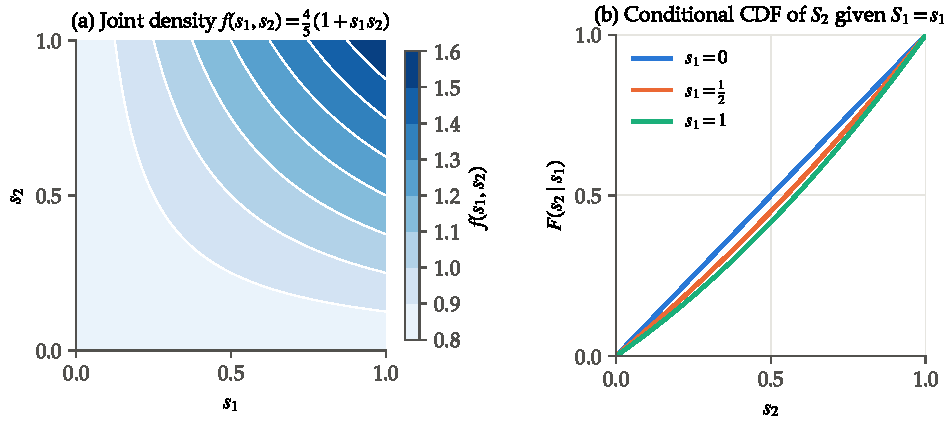
\includegraphics[width=\textwidth]{figures/ch14/affil_example.pdf}
\caption{The affiliated density $f(s_1,s_2)=\frac{4}{5}(1+s_1s_2)$ of \cref{ex:14-affil}(d). Panel (a): the
density is highest where both signals are high. Panel (b): the conditional CDF of $S_2$ shifts down as
$s_1$ rises, so a high signal for one bidder makes high signals of the other more likely.}
\label{fig:14-affil-example}
\end{figure}

Affiliation also has a probabilistic meaning that explains why it is the right condition for auction
theory. Call a set $A\subseteq\R^k$ \emph{increasing} if its indicator function is nondecreasing. Random
variables $\bm Z$ are \emph{associated} if $\Pr(\bm Z\in A\cap B)\ge\Pr(\bm Z\in A)\Pr(\bm Z\in B)$ for all
increasing sets $A$ and $B$. A set $\mathcal{S}\subseteq\R^k$ is a \emph{sublattice} if $\bm z\vee\bm z'$ and
$\bm z\wedge\bm z'$ belong to $\mathcal{S}$ whenever $\bm z$ and $\bm z'$ do. Rectangles and order intervals
$\{\bm z:\bm a\le\bm z\le\bm b\}$ are sublattices. The general definition in the appendix of
\citet{MilgromWeber1982} calls $\bm Z$ affiliated if it is associated conditional on every sublattice. For
variables with a density this coincides with \cref{def:14-affiliation} \citep[Theorem~24]{MilgromWeber1982}.

\begin{proposition}[Association and the covariance inequality]\label{prop:14-association}
\leavevmode
\begin{enumerate}[label=(\alph*)]
  \item The following statements are equivalent \citep[Theorem~22]{MilgromWeber1982}.
  \begin{enumerate}[label=(\roman*)]
    \item $\bm Z$ is associated.
    \item For every pair of nondecreasing functions $g$ and $h$, $\E[g(\bm Z)h(\bm Z)]\ge\E[g(\bm Z)]\,\E[h(\bm
    Z)]$.
    \item For every nondecreasing function $g$ and increasing set $A$, $\E[g(\bm Z)\mid A]\ge\E[g(\bm
    Z)]\ge\E[g(\bm Z)\mid \bar A]$, where $\bar A$ is the complement of $A$.
  \end{enumerate}
  \item $\bm Z$ is affiliated if and only if (ii) and (iii) hold conditional on every sublattice
  $\mathcal{S}$ \citep[Theorem~23]{MilgromWeber1982}. That is, $\E[gh\mid\mathcal{S}]\ge\E[g\mid\mathcal{S}]\,
  \E[h\mid\mathcal{S}]$ and $\E[g\mid A\cap\mathcal{S}]\ge\E[g\mid\mathcal{S}]\ge\E[g\mid\bar A\cap\mathcal{S}]$.
\end{enumerate}
\end{proposition}

\begin{proof}[Proof sketch for part (a)]
To show that (i) implies (ii), take $g$ and $h$ nonnegative and bounded. For a positive integer $K$, define
the step function
\[
g_K(\bm z)=\frac{1}{K}\sum_{l\ge 1}\indic\Bigl\{g(\bm z)>\frac{l}{K}\Bigr\},
\]
which satisfies $g(\bm z)-\frac{1}{K}\le g_K(\bm z)\le g(\bm z)$. Each set $A_l=\{\bm z:g(\bm z)>\frac{l}{K}\}$ is
increasing. Define $h_K$ and increasing sets $B_{l'}$ in the same way. Association gives
\[
\E[g_Kh_K]=\frac{1}{K^2}\sum_{l}\sum_{l'}\Pr(A_l\cap B_{l'})\ \ge\
\frac{1}{K^2}\sum_{l}\sum_{l'}\Pr(A_l)\Pr(B_{l'})=\E[g_K]\,\E[h_K].
\]
Letting $K\to\infty$ proves (ii) for nonnegative bounded functions, and the extension to general $g$ and $h$ is
routine. To show that (ii) implies (iii), take $h=\indic_A$. Then $\E[g\indic_A]\ge\E[g]\Pr(A)$, which is
$\E[g\mid A]\ge\E[g]$. The second inequality follows because $\E[g]=\Pr(A)\E[g\mid A]+\Pr(\bar A)\E[g\mid \bar
A]$ is a weighted average. To show that (iii) implies (i), take $g=\indic_B$. Then $\Pr(B\mid A)\ge\Pr(B)$,
which is association \citep[p.~1119]{MilgromWeber1982}.
\end{proof}

Part (a)(ii) says that nondecreasing functions of affiliated variables are positively correlated. Part (b)
says this remains true conditional on order-interval events, such as the event that the highest rival
signal lies below one's own. This is the form in which affiliation enters equilibrium analysis. The
properties of affiliation used most often are collected next. Write $Y_1\ge Y_2\ge\dots\ge Y_{n-1}$ for the
signals of bidder 1's rivals arranged in decreasing order, so that $Y_1=\max_{j\neq 1}S_j$.

\begin{proposition}[Properties of affiliated variables]\label{prop:14-affil-props}
Let $\bm Z=(Z_1,\dots,Z_k)$ be affiliated.
\begin{enumerate}[label=(\roman*)]
  \item If $g_1,\dots,g_k$ are all nondecreasing or all nonincreasing, then $g_1(Z_1),\dots,g_k(Z_k)$ are
  affiliated \citep[Theorem~3]{MilgromWeber1982}.
  \item Every subvector of $\bm Z$ is affiliated. In particular $Z_1,\dots,Z_{k-1}$ are affiliated
  \citep[Theorem~4]{MilgromWeber1982}.
  \item For every nondecreasing function $H$, the function
  \[
  h(a_1,b_1;\dots;a_k,b_k)=\E\bigl[H(\bm Z)\mid a_1\le Z_1\le b_1,\dots,a_k\le Z_k\le b_k\bigr]
  \]
  is nondecreasing in all its arguments. In particular, $\E[H(\bm Z)\mid Z_1=z_1,\dots,Z_l=z_l]$ is
  nondecreasing in $(z_1,\dots,z_l)$ for each $l=1,\dots,k$ \citep[Theorem~5]{MilgromWeber1982}.
  \item Under \cref{ass:14-mw}, the variables $A_1,\dots,A_m,S_1,Y_1,\dots,Y_{n-1}$ are affiliated
  \citep[Theorem~2]{MilgromWeber1982}.
\end{enumerate}
\end{proposition}

\begin{proof}
Parts (i) and (ii) follow from \cref{prop:14-association}(b)(ii), and part (iii) follows from
\cref{prop:14-association}(b)(iii) \citep[p.~1119]{MilgromWeber1982}. \Cref{sec:14-mw-affil} gives the
arguments. For part (iv), note first that the symmetry of $f$ in the signals implies that the joint density
of $(\bm A,S_1,Y_1,\dots,Y_{n-1})$ is
\begin{equation}\label{eq:14-joint-orderstat}
(n-1)!\;f(\bm a,s_1,y_1,\dots,y_{n-1})\;\indic\{y_1\ge y_2\ge\dots\ge y_{n-1}\}
\end{equation}
\citep[eq.~(4)]{MilgromWeber1982}. The factor $(n-1)!$ counts the orderings of the rivals' signals that
produce the same ordered vector, each of which has the same density by symmetry. The density $f$ is
affiliated by \cref{ass:14-mw}(v). The indicator of any sublattice satisfies \eqref{eq:14-affil-ineq}. If
both points lie in the sublattice, both sides equal one, and otherwise the right side is zero. The set
$\{y_1\ge\dots\ge y_{n-1}\}$ is a sublattice, because the component-wise maximum and minimum of two
nonincreasing sequences are nonincreasing. By \cref{prop:14-affil-char}(ii) the product
\eqref{eq:14-joint-orderstat} is affiliated.
\end{proof}

Parts (iii) and (iv) together imply that $\E[V_1\mid S_1=s,Y_1=y_1,\dots,Y_{n-1}=y_{n-1}]$ is nondecreasing in
all its arguments \citep[p.~1100]{MilgromWeber1982}. In particular, the expected value of the object to
bidder 1 conditional on its own signal and on the highest rival signal,
$v(s,y)=\E[V_1\mid S_1=s,Y_1=y]$, is nondecreasing in both arguments. \Cref{prop:14-mw-spa} shows that $v(s,s)$
is the equilibrium bid in the second-price auction with affiliated values. \Cref{app:math} collects these
results with the other mathematical tools of the book.

\subsection{The winner's curse}\label{sec:14-winners-curse}

Suppose bidders form conditionally independent estimates of a common value $V$, and each estimate is
unbiased. Other things being equal, the bidder with the largest estimate makes the highest bid. The winner
therefore tends to be the bidder who overestimated the value the most. On average, the winner finds that it
had overestimated $V$ \citep[p.~1094]{MilgromWeber1982}. This phenomenon is the \emph{winner's curse}.
Petroleum engineers \citet{CapenClappCampbell1971} claimed that it was responsible for the low profits that
oil companies earned on offshore tracts in the 1960s \citep[p.~1094]{MilgromWeber1982}.

In equilibrium the winner's curse concerns information, and rational bidders do not lose money because of
it. Winning reveals to the winner that its signal was more optimistic than its rivals' signals. This
revelation is ``bad news'' about the value of the object \citep{Milgrom1981}. Rational bidders anticipate it
and condition their bids on the event of winning. The presence of a winner's curse therefore does not imply
that winners regret winning \citep[footnote~7]{AtheyHaile2007}. Losses arise for naive bidders who ignore the
information contained in winning.

The following result makes the bad news precise in the general symmetric model. Recall that
$v(s,y)=\E[V_1\mid S_1=s,Y_1=y]$. In a symmetric equilibrium with a strictly increasing bid function, bidder 1
wins exactly when $Y_1<S_1$.

\begin{proposition}[The bad news in winning]\label{prop:14-wc}
Suppose \cref{ass:14-mw} holds. For every signal $s$ with $\Pr(Y_1<s\mid S_1=s)>0$,
\begin{equation}\label{eq:14-wc}
\E\bigl[V_1\mid S_1=s,\ Y_1<s\bigr]\ \le\ \min\Bigl\{v(s,s),\ \E\bigl[V_1\mid S_1=s\bigr]\Bigr\}.
\end{equation}
Both inequalities are strict if $v(s,y)$ is strictly increasing in $y$ and $\Pr(Y_1<s\mid S_1=s)<1$. Under
private values, $v(s,y)=s$ and both hold with equality.
\end{proposition}

\begin{proof}
By the law of iterated expectations,
\[
\E\bigl[V_1\mid S_1=s,\ Y_1<s\bigr]=\E\bigl[v(s,Y_1)\mid S_1=s,\ Y_1<s\bigr].
\]
By \cref{prop:14-affil-props}(iii) and (iv), $\varphi(y)\equiv v(s,y)$ is nondecreasing in $y$. All expectations
below are conditional on $S_1=s$. For $y<s$ we have $\varphi(y)\le\varphi(s)$, so
\[
\E[\varphi(Y_1)\mid Y_1<s]\ \le\ \varphi(s)=v(s,s),
\]
which is the first inequality. For $y\ge s$ we have $\varphi(y)\ge\varphi(s)$, so
$\E[\varphi(Y_1)\mid Y_1\ge s]\ge\varphi(s)\ge\E[\varphi(Y_1)\mid Y_1<s]$. The unconditional mean is a weighted
average of the two conditional means,
\begin{align*}
\E[V_1\mid S_1=s]=\E[\varphi(Y_1)]
&=\Pr(Y_1<s)\,\E[\varphi(Y_1)\mid Y_1<s]+\Pr(Y_1\ge s)\,\E[\varphi(Y_1)\mid Y_1\ge s]\\
&\ge\Pr(Y_1<s)\,\E[\varphi(Y_1)\mid Y_1<s]+\Pr(Y_1\ge s)\,\E[\varphi(Y_1)\mid Y_1< s]\\
&=\E[\varphi(Y_1)\mid Y_1<s],
\end{align*}
which is the second inequality. If $\varphi$ is strictly increasing, the inequalities between conditional
means are strict whenever both events have positive probability. Under private values,
$\E[V_1\mid S_1=s,Y_1=y]=s$ for all $y$.
\end{proof}

The proof uses affiliation only to guarantee that $v(s,y)$ is nondecreasing in $y$. Interdependence of
values is what creates the curse. In the example $V=\frac{S_1+S_2}{2}$ with independent signals,
$v(s,y)=\frac{s+y}{2}$ rises strictly with $y$, and the curse is present without any dependence between
signals.

The proposition explains why naive bidding fails. Suppose that in a first-price auction every bidder
naively bids its unconditional estimate $\E[V_1\mid S_1=s]$, which increases with $s$. Bidder 1 then wins
exactly when $Y_1<s$. Its expected profit conditional on winning is
\[
\E\bigl[V_1\mid S_1=s,\ Y_1<s\bigr]-\E\bigl[V_1\mid S_1=s\bigr]\ \le\ 0,
\]
which is strictly negative under common values. Naive bidders lose money on average whenever they win.
Equilibrium bids correct for the bad news, as \cref{sec:14-mw-eq} shows.

\begin{example}[The size of the curse with uniform errors]\label{ex:14-wc-uniform}
Consider a mineral rights model with $S_i=V+\epsilon_i$, where the errors $\epsilon_i$ are i.i.d.\ uniform on
$[-\omega,\omega]$ and independent of $V$, and $\omega>0$ is the half-width of the noise. Each signal is an
unbiased estimate, $\E[S_i-V]=0$. The highest signal is $S_{(n:n)}=V+\epsilon_{(n:n)}$. Write
$\epsilon_i=-\omega+2\omega U_i$ with $U_i$ i.i.d.\ uniform on $[0,1]$, so that
$\epsilon_{(n:n)}=-\omega+2\omega U_{(n:n)}$. The maximum of $n$ uniforms has CDF $x^n$ on $[0,1]$, so
\[
\E\bigl[U_{(n:n)}\bigr]=\int_0^1\bigl(1-x^n\bigr)\,dx=1-\frac{1}{n+1}=\frac{n}{n+1}.
\]
Therefore
\begin{equation}\label{eq:14-wc-bias}
\E\bigl[S_{(n:n)}-V\bigr]=-\omega+2\omega\,\frac{n}{n+1}=\omega\,\frac{2n-(n+1)}{n+1}=\omega\,\frac{n-1}{n+1}.
\end{equation}
The bias is zero for $n=1$, equals $\frac{\omega}{3}$ for $n=2$ and rises toward $\omega$ as $n$ grows. The
same steps with $\E[U_{(n-1:n)}]=\frac{n-1}{n+1}$, derived in \eqref{eq:14-uniform-means} below, give
$\E[S_{(n-1:n)}-V]=\omega\frac{n-3}{n+1}$. \Cref{fig:14-wc} plots both.
\end{example}

\begin{figure}[htbp]
\centering
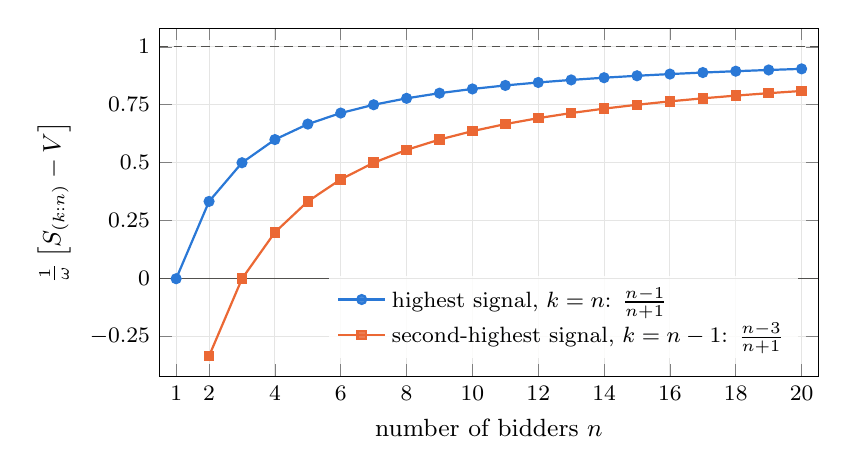
\begin{tikzpicture}
\begin{axis}[
  width=0.82\textwidth, height=6cm,
  xlabel={number of bidders $n$},
  ylabel={$\frac{1}{\omega}\,\E\bigl[S_{(k:n)}-V\bigr]$},
  xmin=0.5, xmax=20.5, ymin=-0.42, ymax=1.08,
  xtick={1,2,4,6,8,10,12,14,16,18,20},
  ytick={-0.25,0,0.25,0.5,0.75,1},
  grid=major, grid style={c14gray!15},
  legend style={at={(0.97,0.05)},anchor=south east,font=\footnotesize,draw=none,fill=white,fill opacity=0.85,text opacity=1},
  legend cell align=left,
  tick label style={font=\footnotesize}, label style={font=\small}]
\addplot[c14gray, thin, forget plot, domain=0.5:20.5] {0};
\addplot[c14gray, densely dashed, forget plot, domain=0.5:20.5] {1};
\addplot[c14blue, thick, mark=*, mark size=1.6pt, domain=1:20, samples=20] {(x-1)/(x+1)};
\addlegendentry{highest signal, $k=n$: $\frac{n-1}{n+1}$}
\addplot[c14orange, thick, mark=square*, mark size=1.5pt, domain=2:20, samples=19] {(x-3)/(x+1)};
\addlegendentry{second-highest signal, $k=n-1$: $\frac{n-3}{n+1}$}
\end{axis}
\end{tikzpicture}
\caption{The winner's curse in the mineral rights model with uniform errors on $[-\omega,\omega]$
(\cref{ex:14-wc-uniform}). Each signal is unbiased, yet the highest of $n$ signals overstates the common
value by $\omega\frac{n-1}{n+1}$ on average. The bias grows with the number of bidders and approaches
$\omega$ (dashed line).}
\label{fig:14-wc}
\end{figure}

More competition makes the bad news in winning worse. With private values, more bidders make each bidder
bid more aggressively (\cref{sec:14-fpa}). With common values, a rational bidder must also correct for a
larger bias in the event of winning. In \cref{ex:14-wc-uniform}, suppose that the prior on $V$ is
\emph{diffuse}, that is, flat over every value that the signals allow. The
second-price equilibrium bid is then $s-\omega\frac{n-2}{n}$, a correction that grows with $n$
(\cref{ex:14-mineral}). The net effect of more bidders on bids is therefore ambiguous under common values.
For the same reason, bids that fall as the number of bidders rises are a misleading test for the winner's
curse \citep{Laffont1997}. \Cref{sec:14-mw-spa} describes a sharper test based on the pivotal value.
\citet{HendricksPorter1988} test whether bidders in the drainage sales of \cref{tab:14-hp-table1} bid in a
way that accounts for the curse (\cref{ch:auction-empirics}).

\begin{remark}[Information aggregation]\label{rem:14-aggregation}
The winner's curse has a positive counterpart. It is tempting to think that the price in a mineral rights
auction conveys no more information than the winner's own estimate. This reasoning is incorrect, since the
winning estimate is the maximum of all estimates and so bounds every loser's estimate
\citep[p.~1094]{MilgromWeber1982}. Let $g(s\mid v)$ be the density of a bidder's estimate when $V=v$. Many
one-parameter families have the MLRP, so that for $v_1<v_2$ the ratio $\frac{g(s\mid v_1)}{g(s\mid v_2)}$
declines as $s$ increases. If this ratio approaches zero, the first-price price with many bidders is a
consistent estimator of $V$, even if no bidder can estimate $V$ closely on its own
\citep{Wilson1977,Milgrom1979}. Prices can thus aggregate dispersed private information.
\end{remark}

\begin{remark}[Privacy versus accuracy of information]\label{rem:14-privacy}
\citet[p.~1094]{MilgromWeber1982} stress that a bidder's expected profit in a mineral rights auction depends
more on the privacy of its information than on its accuracy. In a first-price auction, a bidder whose
information is also available to some other bidder earns zero expected profit in equilibrium
\citep{EngelbrechtWiggansMilgromWeber1983}. This logic fits the near-zero profits of the non-neighbor firms
in the drainage sales, whose information was public and therefore also known to the neighbor firms.
\Cref{prop:14-mw-garbling} proves a related result for second-price auctions.
\end{remark}

\subsection{Order statistics}\label{sec:14-orderstats}

Payments and winning probabilities in auctions are governed by order statistics of bids or values. The
winner of a second-price auction pays the second-highest bid. In a first-price auction a bidder's
probability of winning is the probability that the highest rival bid is lower than its own. This subsection
collects the facts used throughout this chapter and \cref{ch:auction-empirics}. \Cref{sec:B-orderstats}
restates them for reference and adds joint distributions and identification results.

Let $V_1,\dots,V_n$ be i.i.d.\ with continuous CDF $F$ and density $f$. Denote by $V_{(k:n)}$ the $k$-th lowest
of the $n$ draws, so that $V_{(n:n)}$ is the maximum and $V_{(n-1:n)}$ is the second highest. Denote by
$F_{(k:n)}$ its CDF. This indexing from lowest to highest follows \citet[Section~2.1]{AtheyHaile2007}.

\begin{proposition}[Distribution of an order statistic]\label{prop:14-orderstat}
For $k=1,\dots,n$,
\begin{equation}\label{eq:14-orderstat}
F_{(k:n)}(z)=\frac{n!}{(n-k)!\,(k-1)!}\int_0^{F(z)}t^{k-1}(1-t)^{n-k}\,dt,
\end{equation}
and the density of $V_{(k:n)}$ is
\begin{equation}\label{eq:14-orderstat-density}
f_{(k:n)}(z)=\frac{n!}{(n-k)!\,(k-1)!}\,F(z)^{k-1}\bigl(1-F(z)\bigr)^{n-k}f(z).
\end{equation}
\end{proposition}

\begin{proof}
The event $V_{(k:n)}\le z$ occurs if and only if at least $k$ of the $n$ draws are at most $z$. The number of
draws at most $z$ is binomial with parameters $n$ and $F(z)$. Hence
\begin{equation}\label{eq:14-orderstat-binom}
F_{(k:n)}(z)=\sum_{j=k}^{n}\binom{n}{j}F(z)^j\bigl(1-F(z)\bigr)^{n-j}.
\end{equation}
It remains to show that, for $x\in[0,1]$,
\[
\sum_{j=k}^{n}\binom{n}{j}x^j(1-x)^{n-j}=\frac{n!}{(n-k)!\,(k-1)!}\int_0^{x}t^{k-1}(1-t)^{n-k}\,dt.
\]
Both sides vanish at $x=0$, so it suffices that their derivatives agree. Using
$j\binom{n}{j}=n\binom{n-1}{j-1}$ and $(n-j)\binom{n}{j}=n\binom{n-1}{j}$, the derivative of a typical term on the
left is
\[
\frac{d}{dx}\binom{n}{j}x^j(1-x)^{n-j}=n\binom{n-1}{j-1}x^{j-1}(1-x)^{n-j}-n\binom{n-1}{j}x^{j}(1-x)^{n-j-1}.
\]
Summing over $j=k,\dots,n$, the sum telescopes. The second term for $j$ cancels the first term for $j+1$,
and the second term for $j=n$ is zero because $\binom{n-1}{n}=0$. What remains is the first term for $j=k$,
\[
n\binom{n-1}{k-1}x^{k-1}(1-x)^{n-k}=\frac{n!}{(n-k)!\,(k-1)!}\,x^{k-1}(1-x)^{n-k},
\]
which is the derivative of the right side. Formula \eqref{eq:14-orderstat-density} follows by differentiating
\eqref{eq:14-orderstat} with respect to $z$ and applying the chain rule.
\end{proof}

Formula \eqref{eq:14-orderstat} appears as equation (5) in \citet{AtheyHaile2002}. The density
\eqref{eq:14-orderstat-density} has a direct interpretation. One draw falls at $z$, $k-1$ draws fall below
and $n-k$ fall above, and the multinomial coefficient $\frac{n!}{(k-1)!\,1!\,(n-k)!}$ counts the ways of
assigning the draws to these three groups.

From bidder $i$'s point of view, the most important order statistic is the highest of its rivals' values,
$Y_1=\max_{j\neq i}V_j$. Under independence, $Y_1\le y$ if and only if every rival's value is at most $y$, so
\begin{equation}\label{eq:14-highest-rival}
F_{Y_1}(y)=F(y)^{n-1},\qquad f_{Y_1}(y)=(n-1)F(y)^{n-2}f(y).
\end{equation}
This is the case $k=n-1$ of \eqref{eq:14-orderstat} applied to the sample of $n-1$ rivals, since
$Y_1=V_{(n-1:n-1)}$ in that sample. If all bidders use the same strictly increasing bid function, a bidder
with value $v$ wins with probability $F(v)^{n-1}$.

The transaction price in second-price and ascending auctions is the second-highest value. Its CDF is
\begin{equation}\label{eq:14-second-highest}
F_{(n-1:n)}(v)=nF(v)^{n-1}\bigl(1-F(v)\bigr)+F(v)^n=\Lambda_n\bigl(F(v)\bigr),\qquad
\Lambda_n(x)\equiv nx^{n-1}(1-x)+x^n.
\end{equation}
We derive it in two ways. By counting, $V_{(n-1:n)}\le v$ if and only if at least $n-1$ of the $n$ draws are at
most $v$. Either all $n$ draws are at most $v$, with probability $F(v)^n$, or exactly $n-1$ are, with
probability $nF(v)^{n-1}(1-F(v))$. The factor $n$ counts the choices of the single draw above $v$.
Alternatively, set $k=n-1$ in \eqref{eq:14-orderstat}:
\begin{align*}
F_{(n-1:n)}(v)&=\frac{n!}{1!\,(n-2)!}\int_0^{F(v)}t^{n-2}(1-t)\,dt\\
&=n(n-1)\left[\frac{F(v)^{n-1}}{n-1}-\frac{F(v)^n}{n}\right]\\
&=nF(v)^{n-1}-(n-1)F(v)^n\\
&=nF(v)^{n-1}\bigl(1-F(v)\bigr)+F(v)^n.
\end{align*}

The map $\Lambda_n$ is a strictly increasing bijection of $[0,1]$. Indeed $\Lambda_n(0)=0$, $\Lambda_n(1)=1$,
and writing $\Lambda_n(x)=nx^{n-1}-(n-1)x^n$,
\[
\Lambda_n'(x)=n(n-1)x^{n-2}-n(n-1)x^{n-1}=n(n-1)x^{n-2}(1-x)>0\qquad\text{for }x\in(0,1).
\]
Consequently,
\begin{equation}\label{eq:14-lambda-inverse}
F(v)=\Lambda_n^{-1}\bigl(F_{(n-1:n)}(v)\bigr),
\end{equation}
so the distribution of the second-highest value determines $F$. The same argument applies to any order
statistic, because the right side of \eqref{eq:14-orderstat} is strictly increasing in $F(z)$.
\citet[Theorem~1]{AtheyHaile2002} use this fact to show that $F$ is identified from transaction prices
alone, a result developed in \cref{ch:auction-empirics}.

When $F$ is uniform on $[0,1]$, the density of $V_{(k:n)}$ is
$\frac{n!}{(n-k)!\,(k-1)!}x^{k-1}(1-x)^{n-k}$, a beta density with parameters $k$ and $n-k+1$. Using
$\int_0^1x^a(1-x)^b\,dx=\frac{a!\,b!}{(a+b+1)!}$ for nonnegative integers $a$ and $b$, its mean is
\begin{equation}\label{eq:14-uniform-means}
\E\bigl[V_{(k:n)}\bigr]=\frac{n!}{(n-k)!\,(k-1)!}\int_0^1x^{k}(1-x)^{n-k}\,dx
=\frac{n!}{(n-k)!\,(k-1)!}\cdot\frac{k!\,(n-k)!}{(n+1)!}=\frac{k}{n+1}.
\end{equation}
The $n$ draws split $[0,1]$ into $n+1$ segments of equal expected length. In particular
$\E[V_{(n:n)}]=\frac{n}{n+1}$ and $\E[V_{(n-1:n)}]=\frac{n-1}{n+1}$. \Cref{fig:14-orderstat} plots the
densities of the two highest of four uniform values, together with the density of the highest of three
rival values.

\begin{figure}[htbp]
\centering
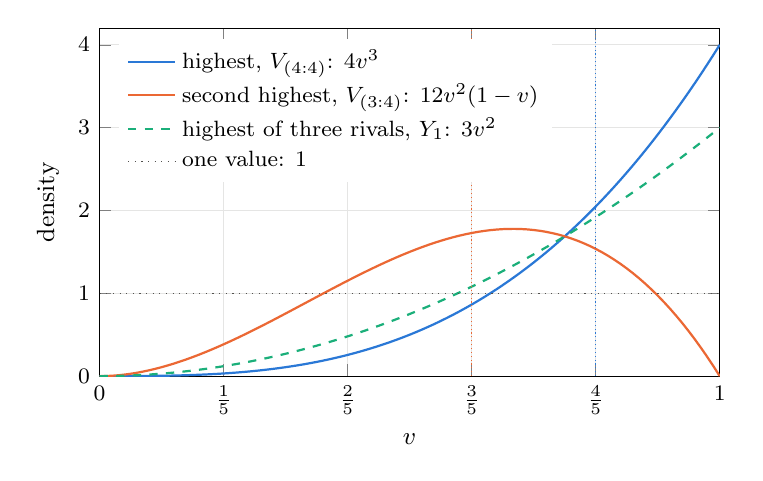
\begin{tikzpicture}
\begin{axis}[
  width=0.78\textwidth, height=6cm,
  xlabel={$v$}, ylabel={density},
  xmin=0, xmax=1, ymin=0, ymax=4.2,
  xtick={0,0.2,0.4,0.6,0.8,1},
  xticklabels={$0$,$\frac{1}{5}$,$\frac{2}{5}$,$\frac{3}{5}$,$\frac{4}{5}$,$1$},
  grid=major, grid style={c14gray!15},
  legend style={at={(0.03,0.97)},anchor=north west,font=\footnotesize,draw=none},
  legend cell align=left,
  tick label style={font=\footnotesize}, label style={font=\small}]
\addplot[c14blue, thick, domain=0:1, samples=101] {4*x^3};
\addlegendentry{highest, $V_{(4:4)}$: $4v^3$}
\addplot[c14orange, thick, domain=0:1, samples=101] {12*x^2*(1-x)};
\addlegendentry{second highest, $V_{(3:4)}$: $12v^2(1-v)$}
\addplot[c14aqua, thick, dashed, domain=0:1, samples=101] {3*x^2};
\addlegendentry{highest of three rivals, $Y_1$: $3v^2$}
\addplot[c14gray, thin, dotted, domain=0:1] {1};
\addlegendentry{one value: $1$}
\draw[c14blue, densely dotted] (axis cs:0.8,0) -- (axis cs:0.8,4.2);
\draw[c14orange, densely dotted] (axis cs:0.6,0) -- (axis cs:0.6,4.2);
\end{axis}
\end{tikzpicture}
\caption{Densities of order statistics of $n=4$ values drawn from the uniform distribution on $[0,1]$. The
vertical lines mark the means $\E[V_{(4:4)}]=\frac{4}{5}$ and $\E[V_{(3:4)}]=\frac{3}{5}$ from
\eqref{eq:14-uniform-means}. The dashed curve is the density of the highest of a bidder's three rivals,
$f_{Y_1}(v)=3v^2$, from \eqref{eq:14-highest-rival}.}
\label{fig:14-orderstat}
\end{figure}

Finally, two facts about expectations are used repeatedly. For a nonnegative random variable $X$,
$\E[X]=\int_0^\infty\Pr(X>x)\,dx$. For values supported on $[0,\bar v]$, this gives
\begin{equation}\label{eq:14-mean-second}
\E\bigl[V_{(n-1:n)}\bigr]=\int_0^{\bar v}\Bigl[1-\Lambda_n\bigl(F(v)\bigr)\Bigr]dv.
\end{equation}
When signals are dependent, the order statistics of the rivals' signals have the joint density
\eqref{eq:14-joint-orderstat}. In the descending notation of \citet{MilgromWeber1982}, $Y_k$ is the $k$-th
highest of the $n-1$ rivals' signals, which is $S_{(n-k:n-1)}$ in the ascending notation applied to the
rivals' sample.

\section{Second-Price and Ascending Auctions with Private Values}\label{sec:14-spa}

We now solve the simplest auctions in the simplest information structure. Throughout this section values
are private, so each bidder knows its own value $v_i$. The first two results allow any joint distribution
of values. The third specializes to the SIPV model to compute revenue and surplus.

\subsection{Truthful bidding in the second-price auction}\label{sec:14-spa-dominance}

Consider a second-price sealed-bid auction with reserve price $r\ge 0$. Fix bidder $i$ with value $v_i$ and
any bids of its rivals. Let
\[
\tilde m=\max\Bigl\{r,\ \max_{j\neq i}b_j\Bigr\}
\]
be the \emph{price to beat}, the lowest price at which bidder $i$ can win. By \eqref{eq:14-payoff-spa}, a
bid $b\ge r$ wins when it exceeds every rival bid, and the winner pays $\tilde m$. Bidder $i$'s payoff from
such a bid is
\begin{equation}\label{eq:14-spa-payoff}
u_i(b;\bm b_{-i})=(v_i-\tilde m)\,\indic\Bigl\{b>\max_{j\neq i}b_j\Bigr\},
\end{equation}
and its payoff from a bid below $r$ is zero. A bid above $\tilde m$ therefore wins, and a bid below
$\tilde m$ loses. A bid $b=\tilde m$ wins at price $r$ when every rival bid is below $r$. Otherwise it ties
with the highest rival bid, and \eqref{eq:14-payoff-spa} counts the tie as a loss. Any other tie-breaking
rule leaves the argument below unchanged, because a tied bid still earns either $v_i-\tilde m$ or zero.
The payment does not depend on bidder $i$'s own bid, which
only determines whether $i$ wins. A strategy is \emph{weakly dominant} if it does at least as well as any other
strategy against every profile of rivals' bids. It must also do strictly better than each alternative
against some profile. Bids below $r$ are all rejected, so we treat them as one action, not bidding.

\begin{proposition}[Vickrey 1961]\label{prop:14-spa-dominant}
With private values, bidding one's value, $b_i=v_i$, is a weakly dominant strategy in the second-price
sealed-bid auction with any reserve price. The result requires no assumption on the number of bidders, on
the joint distribution of values or on the bidder's knowledge of that distribution.
\end{proposition}

\begin{proof}
Fix the rivals' bids, and hence $\tilde m$. Every bid leads to one of two outcomes. Bidder $i$ either wins
and receives $v_i-\tilde m$, or loses and receives zero. The bid $b=v_i$ wins when $v_i>\tilde m$ and loses
when $v_i<\tilde m$. When $v_i=\tilde m$, both outcomes give zero. Hence the bid $v_i$ yields
\[
u_i(v_i;\bm b_{-i})=\max\{v_i-\tilde m,\ 0\},
\]
the larger of the two possible payoffs. No bid does better against any $\tilde m$. If $v_i<r$, the bid
$v_i$ is rejected and earns zero, which is optimal because any winning bid pays at least $r>v_i$.

Every other bid does strictly worse against some $\tilde m$, with two exceptions. For $v_i<r$, every bid
below $r$ is the same action as bidding $v_i$. For $v_i=r$, not bidding earns the same as bidding $v_i$
against every profile, so we treat the two as one action. A bid $b>v_i$ wins when
$v_i<\tilde m<b$ and then earns $v_i-\tilde m<0$, where bidding $v_i$ would have earned zero. A bid $b<v_i$
loses when $b<\tilde m<v_i$ and earns zero, where bidding $v_i$ would have earned $v_i-\tilde m>0$. Hence
$b_i=v_i$ is weakly dominant \citep{Vickrey1961}.
\end{proof}

\Cref{fig:14-spa-payoff} draws the three cases. Bidding one's value is optimal against every possible price
to beat, so a bidder needs no forecast of rivals' behavior. This is why the result needs neither symmetry,
nor independence, nor common knowledge of the distribution of values.

\begin{figure}[htbp]
\centering
\begin{tikzpicture}
\pgfplotsset{spapanel/.style={
  scale only axis, width=3.75cm, height=3.0cm, axis lines=middle, xmin=0, xmax=1.08, ymin=-0.38, ymax=0.72,
  xtick=\empty, ytick=\empty, xlabel={$\tilde m$}, xlabel style={anchor=west,font=\small},
  title style={font=\small,yshift=4pt}, clip=false}}
\begin{axis}[spapanel, name=pA, title={(a) underbidding, $b<v$}]
  \fill[c14orange!35] (axis cs:0.35,0) -- (axis cs:0.6,0) -- (axis cs:0.35,0.25) -- cycle;
  \addplot[c14gray, densely dashed, domain=0.35:0.6] {0.6-x};
  \addplot[c14blue, very thick, domain=0:0.35] {0.6-x};
  \addplot[c14blue, very thick, domain=0.35:1.0] {0};
  \node[font=\footnotesize,anchor=south west] at (axis cs:0.42,0.18) {forgone gain};
  \node[font=\footnotesize,anchor=north] at (axis cs:0.35,0) {$b$};
  \node[font=\footnotesize,anchor=north] at (axis cs:0.6,0) {$v$};
  \node[font=\small,anchor=east] at (axis cs:0,0.62) {payoff};
\end{axis}
\begin{axis}[spapanel, name=pB, at={($(pA.east)+(0.75cm,0)$)}, anchor=west, title={(b) truthful, $b=v$}]
  \addplot[c14blue, very thick, domain=0:0.6] {0.6-x};
  \addplot[c14blue, very thick, domain=0.6:1.0] {0};
  \node[font=\footnotesize,anchor=south west] at (axis cs:0.30,0.36) {$\max\{v-\tilde m,0\}$};
  \node[font=\footnotesize,anchor=north] at (axis cs:0.6,0) {$v=b$};
\end{axis}
\begin{axis}[spapanel, name=pC, at={($(pB.east)+(0.75cm,0)$)}, anchor=west, title={(c) overbidding, $b>v$}]
  \fill[c14orange!35] (axis cs:0.6,0) -- (axis cs:0.85,0) -- (axis cs:0.85,-0.25) -- cycle;
  \addplot[c14blue, very thick, domain=0:0.85] {0.6-x};
  \addplot[c14blue, very thick, domain=0.85:1.0] {0};
  \node[font=\footnotesize,anchor=north east] at (axis cs:0.6,0) {$v$};
  \node[font=\footnotesize,anchor=north] at (axis cs:0.85,-0.25) {$b$};
  \node[font=\footnotesize,anchor=west] at (axis cs:0.88,-0.14) {added loss};
\end{axis}
\end{tikzpicture}
\caption{Payoff in a second-price auction as a function of the price to beat $\tilde m$, for a bidder with
value $v$. Truthful bidding (b) attains $\max\{v-\tilde m,0\}$ for every $\tilde m$. Underbidding (a) loses
the auction when $b<\tilde m<v$ and forgoes the shaded gains. Overbidding (c) wins when $v<\tilde m<b$ and
adds the shaded losses.}
\label{fig:14-spa-payoff}
\end{figure}

\begin{remark}[What the result does and does not need]\label{rem:14-spa-needs}
The proof compares only the sign of $v_i-\tilde m$. It therefore holds for any increasing utility of money
$\mathcal{U}$ with $\mathcal{U}(0)=0$, so a risk-averse bidder also bids its value (\cref{sec:14-fpa} uses
this). The proof does require private values. With interdependent values a bidder does not know its value
when it bids, and the payoff $v_i-\tilde m$ is replaced by an expectation that depends on what winning at
price $\tilde m$ reveals. \Cref{prop:14-mw-spa} shows that the equilibrium bid then becomes $v(s,s)$.
\end{remark}

\begin{remark}[Other equilibria]\label{rem:14-spa-other}
Truthful bidding is the only weakly undominated strategy, up to the equivalence of all bids below $r$.
The second-price auction has other Bayesian Nash equilibria in weakly dominated strategies. Let values lie in $[\underline v,\bar v]$ and set
$r=\underline v$. Suppose bidder 1 bids $\bar v$ whatever its value and every other bidder bids
$\underline v$. Bidder 1 always wins and pays $\underline v\le v_1$, and no other bid gives it more. Any other
bidder could win only by bidding above $\bar v$, and would then pay $\bar v\ge v_j$. Hence no bidder gains by
deviating. This equilibrium misallocates the object whenever a rival values it more than bidder 1, and it
yields revenue $\underline v$. Following \citet[Section~2.2]{AtheyHaile2007}, we restrict attention to
equilibria in weakly undominated strategies.
\end{remark}

\begin{remark}[Second-price auctions in practice]
Pure second-price sealed-bid auctions are uncommon in practice \citep[footnote~2]{AtheyHaile2007}. The
proxy bidding system of eBay has the flavor of a second-price auction. A bidder submits a maximum, and the
system bids on its behalf up to that maximum, so the winner pays roughly the second-highest maximum. Bidders
can usually observe and respond to the bids of at least some rivals, however, as in an ascending auction.
\end{remark}

\subsection{The English auction with private values}\label{sec:14-english-pv}

The same logic solves the button auction of \cref{def:14-button}. The dynamic structure adds nothing under
private values, because a bidder has nothing to learn from rivals' exits about its own value.

\begin{proposition}[English auction with private values]\label{prop:14-english-dominant}
With private values, consider the English (button) auction with any reserve price. For each bidder, the
strategy of remaining active until the price reaches $v_i$, whatever the history of exits, is weakly
dominant. When all bidders follow it, the bidder with the highest value wins whenever that value is at
least $r$. The winner pays
\begin{equation}\label{eq:14-english-price}
P=\max\bigl\{V_{(n-1:n)},\ r\bigr\}\qquad\text{if }V_{(n:n)}\ge r,
\end{equation}
where $V_{(n:n)}$ and $V_{(n-1:n)}$ are the highest and second-highest values. If $V_{(n:n)}<r$, the object
is not sold. The second-price sealed-bid auction with truthful bids produces the same allocation and price.
\end{proposition}

\begin{proof}
Fix bidder $i$, the strategies of its rivals and the realization of the rivals' values. Rivals observe the
price and the set of active bidders. As long as bidder $i$ is active, its plans for the future do not affect
what the rivals observe. Hence the path of rival exits up to the moment bidder $i$ quits is the same for
every strategy of bidder $i$. Let $\tilde m$ be the price at which the last rival would quit along this
path. Set $\tilde m=r$ if no rival is active at the reserve price, and $\tilde m=+\infty$ if some rival never
quits. Any strategy of bidder $i$ results in some quitting price $d$ along this path, which may depend on the
rival exits it observes. Bidder $i$ wins if $d>\tilde m$ and then pays $\tilde m$, so its payoff is
\[
(v_i-\tilde m)\,\indic\{d>\tilde m\}.
\]
As in \eqref{eq:14-spa-payoff}, bidder $i$ either wins and receives $v_i-\tilde m$ or loses and receives
zero. By the argument in the proof of \cref{prop:14-spa-dominant},
quitting at $d=v_i$ yields $\max\{v_i-\tilde m,0\}$, the largest payoff available against any $\tilde m$.
This holds for every profile of rival strategies and every realization of rival values, so the strategy is
weakly dominant.

When every bidder follows this strategy, bidders quit in increasing order of their values. The auction
ends when the bidder with the second-highest value quits at price $V_{(n-1:n)}$, or at $r$ if that value is
below $r$. The bidder with the highest value wins, provided its value is at least $r$. The second-price
auction with truthful bids gives the same winner and the same price.
\end{proof}

Under private values the English and second-price auctions are therefore equivalent in a weaker sense than
strategic equivalence \citep[p.~1091]{MilgromWeber1982}. Each has a unique dominant strategy equilibrium,
and the two equilibria produce the same outcome. The equilibrium strategy is the one recorded in equation
(2.6) of \citet{AtheyHaile2007}, under which each bidder bids up to its value. The argument requires that
each bidder know its value. It fails when the value depends on what others know, as with minerals of
unknown quantity or a painting to be resold at an unknown price.

An allocation is \emph{efficient} if the object goes to the bidder who values it most. Both auctions
allocate efficiently whenever some bidder values the object above $r$. Without a reserve price the
outcome is always efficient, or Pareto optimal in the terms of \citet[p.~1091]{MilgromWeber1982}. This conclusion does not
depend on symmetry or independence. In symmetric models the Dutch and
first-price auctions also allocate efficiently. With asymmetric bidders they need not
(\cref{sec:14-asym}). Bidders also need no knowledge of rivals' value distributions or of the number of
rivals. \citet[Section~2.1]{AtheyHaile2007} note that the common knowledge assumptions are inconsequential
for ascending auctions with private values.

\subsection{Revenue and surplus with symmetric independent private values}\label{sec:14-spa-revenue}

We now compute expected revenue and bidders' expected surplus in the SIPV model. Values are i.i.d.\ with CDF
$F$ and density $f$ on $[\underline v,\bar v]$, with $\underline v\ge 0$, and the reserve price satisfies
$r\in[\underline v,\bar v]$. By \cref{prop:14-english-dominant} the formulas apply to both the second-price
and the English auction.

\begin{proposition}[Revenue and surplus in the second-price and English auctions]\label{prop:14-spa-revenue}
Consider the SIPV model with reserve price $r$.
\begin{enumerate}[label=(\roman*)]
  \item Expected revenue is
  \begin{equation}\label{eq:14-spa-revenue}
  R(r)=r\bigl[1-F(r)^n\bigr]+\int_r^{\bar v}\Bigl[1-\Lambda_n\bigl(F(v)\bigr)\Bigr]dv.
  \end{equation}
  Without a binding reserve price, $r=\underline v$, this equals
  $\E[V_{(n-1:n)}]=\underline v+\int_{\underline v}^{\bar v}\bigl[1-\Lambda_n(F(v))\bigr]dv$.
  \item A bidder with value $v\ge r$ wins with probability $Q(v)=F(v)^{n-1}$, makes the expected payment
  \begin{equation}\label{eq:14-spa-payment}
  m(v)=rF(r)^{n-1}+\int_r^{v}y\,dF(y)^{n-1}=vF(v)^{n-1}-\int_r^{v}F(y)^{n-1}\,dy,
  \end{equation}
  and earns the expected surplus
  \begin{equation}\label{eq:14-spa-surplus}
  \pi(v)=vQ(v)-m(v)=\int_r^{v}F(y)^{n-1}\,dy.
  \end{equation}
  Bidders with values below $r$ earn zero.
  \item If values are uniform on $[0,1]$, then
  \begin{equation}\label{eq:14-spa-uniform}
  R(r)=\frac{n-1}{n+1}+r^n-\frac{2n}{n+1}\,r^{n+1},\qquad \pi(v)=\frac{v^n-r^n}{n}.
  \end{equation}
  Without a reserve price, revenue is $\frac{n-1}{n+1}$, each bidder's ex ante expected surplus is
  $\frac{1}{n(n+1)}$, and total surplus is $\frac{n}{n+1}$.
\end{enumerate}
\end{proposition}

\begin{proof}
(i) The price is $P=\max\{V_{(n-1:n)},r\}$ if $V_{(n:n)}\ge r$ and zero otherwise. Since $P\ge 0$,
$\E[P]=\int_0^\infty\Pr(P>p)\,dp$. For $p<r$, $P>p$ if and only if the object is sold, that is,
$V_{(n:n)}\ge r$. This has probability $1-F(r)^n$. For $p\ge r$, $P>p$ if and only if $V_{(n-1:n)}>p$, since
$V_{(n-1:n)}>p\ge r$ already implies $V_{(n:n)}>r$. By \eqref{eq:14-second-highest} this has probability
$1-\Lambda_n(F(p))$, which is zero for $p\ge\bar v$. Hence
\[
R(r)=\int_0^{r}\bigl[1-F(r)^n\bigr]dp+\int_r^{\bar v}\Bigl[1-\Lambda_n\bigl(F(p)\bigr)\Bigr]dp,
\]
which is \eqref{eq:14-spa-revenue}. With $r=\underline v$ we have $F(r)=0$, and the first term equals
$\underline v$.

(ii) A bidder with value $v\ge r$ wins if and only if $Y_1<v$. By \eqref{eq:14-highest-rival},
$Q(v)=F(v)^{n-1}$. When it wins, it pays $\max\{Y_1,r\}$. Hence
\[
m(v)=\E\bigl[\max\{Y_1,r\}\,\indic\{Y_1<v\}\bigr]=rF(r)^{n-1}+\int_r^{v}y\,dF(y)^{n-1}.
\]
Integration by parts gives
\[
\int_r^{v}y\,dF(y)^{n-1}=vF(v)^{n-1}-rF(r)^{n-1}-\int_r^{v}F(y)^{n-1}\,dy.
\]
Substituting, $m(v)=vF(v)^{n-1}-\int_r^vF(y)^{n-1}dy$, and therefore
$\pi(v)=vF(v)^{n-1}-m(v)=\int_r^vF(y)^{n-1}dy$.

(iii) With $F(v)=v$ on $[0,1]$ we have $\Lambda_n(v)=nv^{n-1}-(n-1)v^n$. Then
\[
\int_r^1\bigl[1-\Lambda_n(v)\bigr]dv=(1-r)-(1-r^n)+\frac{n-1}{n+1}\bigl(1-r^{n+1}\bigr).
\]
Adding $r(1-r^n)$ gives
\begin{align*}
R(r)&=r-r^{n+1}+r^n-r+\frac{n-1}{n+1}-\frac{n-1}{n+1}\,r^{n+1}\\
&=\frac{n-1}{n+1}+r^n-\frac{2n}{n+1}\,r^{n+1}.
\end{align*}
With $r=0$, revenue is $\frac{n-1}{n+1}$, which matches $\E[V_{(n-1:n)}]$ in \eqref{eq:14-uniform-means}. The
surplus is $\pi(v)=\int_r^vy^{n-1}dy=\frac{v^n-r^n}{n}$. With $r=0$, the ex ante surplus is
$\E[\pi(V)]=\frac{1}{n}\int_0^1v^n\,dv=\frac{1}{n(n+1)}$. Total surplus is $\E[V_{(n:n)}]=\frac{n}{n+1}$,
because the allocation is efficient. As a check, revenue plus the surplus of all $n$ bidders is
$\frac{n-1}{n+1}+\frac{n}{n(n+1)}=\frac{n}{n+1}$.
\end{proof}

Formula \eqref{eq:14-spa-surplus} is the first appearance of a general principle. The interim surplus of a
bidder depends only on the probabilities of winning of lower types,
\[
\pi(v)=\pi(r)+\int_r^{v}Q(y)\,dy.
\]
\Cref{sec:14-ret} shows that this relation holds in every auction and is the source of revenue
equivalence.

The reserve price trades off two effects. Differentiating \eqref{eq:14-spa-uniform},
\[
R'(r)=nr^{n-1}-2nr^n=nr^{n-1}(1-2r).
\]
Revenue rises with $r$ up to $r=\frac{1}{2}$ and falls afterward, for every $n$. A higher reserve raises the
price when exactly one bidder values the object above $r$. It loses the sale when nobody does. For uniform
values, \cref{sec:14-optimal} shows that $r=\frac{1}{2}$ maximizes expected revenue among all selling
mechanisms, a result due to \citet{Myerson1981} and \citet{RileySamuelson1981}. \Cref{tab:14-spa-uniform}
evaluates the formulas of \cref{prop:14-spa-revenue} for several numbers of bidders.

\begin{table}[htbp]
\centering
\caption{Second-price and English auctions with uniform values on $[0,1]$}\label{tab:14-spa-uniform}
\small
\begin{tabular}{@{}ccccccccc@{}}
\toprule
 & \multicolumn{2}{c}{Expected revenue} & \multicolumn{2}{c}{Total surplus} &
 \multicolumn{2}{c}{Surplus per bidder} & Probability \\
\cmidrule(lr){2-3}\cmidrule(lr){4-5}\cmidrule(lr){6-7}
$n$ & $r=0$ & $r=\frac{1}{2}$ & $r=0$ & $r=\frac{1}{2}$ & $r=0$ & $r=\frac{1}{2}$ & of no sale, $r=\frac{1}{2}$ \\
\midrule
2  & 0.3333 & 0.4167 & 0.6667 & 0.5833 & 0.1667 & 0.0833 & 0.2500 \\
3  & 0.5000 & 0.5313 & 0.7500 & 0.7031 & 0.0833 & 0.0573 & 0.1250 \\
5  & 0.6667 & 0.6719 & 0.8333 & 0.8203 & 0.0333 & 0.0297 & 0.0313 \\
10 & 0.8182 & 0.8183 & 0.9091 & 0.9086 & 0.0091 & 0.0090 & 0.0010 \\
\bottomrule
\end{tabular}

\smallskip
\begin{minipage}{0.92\textwidth}
\footnotesize Notes: Computed from \cref{prop:14-spa-revenue}. Revenue is
$\frac{n-1}{n+1}+r^n-\frac{2n}{n+1}r^{n+1}$, total surplus is $\frac{n}{n+1}(1-r^{n+1})$, surplus per bidder is
$\frac{1}{n}\bigl[\frac{1-r^{n+1}}{n+1}-r^n(1-r)\bigr]$ and the probability of no sale is $r^n$. With $n=2$
the exact values are $\frac{1}{3}$ and $\frac{5}{12}$ for revenue, $\frac{2}{3}$ and $\frac{7}{12}$ for
total surplus and $\frac{1}{6}$ and $\frac{1}{12}$ for surplus per bidder.
\end{minipage}
\end{table}

Three patterns stand out in \cref{tab:14-spa-uniform}. Revenue rises and bidder surplus falls as the number
of bidders grows, because the second-highest value moves toward the highest. With two bidders, the reserve
price raises revenue from $\frac{1}{3}$ to $\frac{5}{12}$, a gain of 25 percent. Total surplus falls from
$\frac{2}{3}$ to $\frac{7}{12}$, because the object goes unsold with probability $\frac{1}{4}$. As $n$ grows,
the gain from the reserve price vanishes, since it becomes unlikely that fewer than two bidders value the
object above $r$.

\subsection{What second-price and English auctions reveal}\label{sec:14-spa-data}

The dominant strategy results have strong empirical implications, which \cref{ch:auction-empirics}
develops. In a second-price auction with private values, bids equal values. If all bids from SIPV auctions
are observed, they are i.i.d.\ draws from $F$, and their empirical distribution estimates $F$ directly. In
an English auction the winner's value is never revealed, because the auction stops when the bidder with the
second-highest value quits. The transaction price is the most reliably observed outcome. By
\eqref{eq:14-english-price} it equals $V_{(n-1:n)}$ when the reserve price does not bind. Because $\Lambda_n$ is
strictly increasing, the distribution of transaction prices in auctions with $n$ bidders determines $F$
through \eqref{eq:14-lambda-inverse} \citep[Theorem~1]{AtheyHaile2002}.

Both arguments rest on private values and on the button model. With interdependent values, bids no longer
equal values (\cref{sec:14-mw-eq}). In real open-outcry auctions, recorded bids need not equal the prices at
which bidders would quit (\cref{sec:14-formats-english}). With asymmetric independent private values,
truthful bidding remains dominant and the allocation remains efficient. Revenue is then the expected
second-highest of values drawn from different distributions (\cref{sec:14-asym}).

\section{First-Price Auctions with Symmetric Independent Private Values}\label{sec:14-fpa}

In a first-price sealed-bid auction each bidder submits one sealed bid, the highest bid wins, and the winner pays its own bid. Unlike in the second-price auction of \cref{sec:14-spa}, no bidder has a dominant strategy in this format. The best bid depends on how aggressively the rivals bid, so the analysis requires an equilibrium of a game of incomplete information. This section solves that game in the benchmark model of symmetric independent private values (SIPV). We derive the equilibrium bid function in two ways and study its shape in closed-form examples. We then rewrite the equilibrium condition in terms of the distribution of bids, which is the starting point of the empirical methods in \cref{ch:auction-empirics}. The section ends with reserve prices, multiple equilibria, and risk-averse bidders.

\subsection{The first-price auction as a Bayesian game}\label{sec:14-fpa-game}

We maintain the following assumption throughout \cref{sec:14-fpa}, except where we relax risk neutrality in \cref{sec:14-fpa-risk}.

\begin{assumption}[Symmetric independent private values]\label{ass:14-sipv}
(i) There are $n\ge 2$ risk-neutral bidders and one indivisible object.
(ii) Bidder $i$ privately observes its value $V_i$.
(iii) The values $V_1,\dots,V_n$ are independent draws from a distribution $F$ with support $[\underline v,\bar v]$, where $0\le\underline v<\bar v\le\infty$. The distribution has a finite mean and a continuous density $f$ that is strictly positive on $(\underline v,\bar v)$.
(iv) A losing bidder receives zero, whoever wins.
(v) The number of bidders $n$ and the distribution $F$ are common knowledge.
\end{assumption}

The first-price auction (FPA) under \cref{ass:14-sipv} is a Bayesian game. The players are the $n$ bidders. A player's type is its value $v_i$, and types are drawn from the product distribution $\prod_{i=1}^n F(v_i)$. An action is a bid $b_i\in\R$. The seller may announce a \emph{reserve price} $r\ge\underline v$, which is the lowest bid it accepts. A bidder who does not wish to buy at a price of $r$ or more submits no bid, and we treat this as a bid below $r$. When bidder $i$'s bid is accepted, its payoff is
\begin{equation}\label{eq:14-fpa-payoff}
u_i(b_i,\bm b_{-i};v_i)=(v_i-b_i)\,\indic\Big(b_i>\max_{j\neq i}b_j\Big).
\end{equation}
The payoff depends on the rivals only through their bids. This is the content of private values together with the absence of externalities. Ties are broken at random. They occur with probability zero in every equilibrium we study, because equilibrium bids have continuous distributions.

A \emph{strategy} for bidder $i$ is a bid function $\beta_i$ that maps each value into a bid. We write $B_j=\beta_j(V_j)$ for bidder $j$'s random bid.

\begin{definition}[Bayesian Nash equilibrium]\label{def:14-bne}
A strategy profile $(\beta_1,\dots,\beta_n)$ is a \emph{Bayesian Nash equilibrium} (BNE) if, for every bidder $i$ and every value $v_i$, the bid $\beta_i(v_i)$ maximizes
\[
\E\Big[(v_i-b)\,\indic\Big(b>\max_{j\neq i}\beta_j(V_j)\Big)\Big]
\]
over $b$. The expectation is over the rivals' values. The equilibrium is \emph{symmetric} if $\beta_i=\beta$ for every $i$.
\end{definition}

Each bidder best-responds to the strategies of the others. It knows its own value, treats the rivals' values as random, and shares with them the knowledge of $F$ and of the payoff function.

Consider a bidder who values the object at \$10. If it bids \$10, its payoff is zero whether it wins or loses. If it bids \$9, it earns \$1 each time the bid wins. Any bid with a positive chance of winning beats bidding one's value, so equilibrium bids lie below values. We call the gap $v_i-b_i$ the \emph{shading} of the bid. How much to shade is a trade-off. A lower bid raises the profit conditional on winning but lowers the probability of winning. Let
\[
H(b)=\Pr\Big(\max_{j\neq i}B_j<b\Big)
\]
denote the probability that a bid $b$ wins. Bidder $i$ then maximizes
\begin{equation}\label{eq:14-fpa-objective}
U(b;v_i)=(v_i-b)\,H(b).
\end{equation}
This is the problem of a monopsonist that buys one unit. The value plays the role of the buyer's marginal value, the bid is the price, and $H$ is the residual supply curve. We make the analogy precise in \cref{sec:14-fpa-G}.

Independence implies that $H$ is the same function for every value $v_i$. Bidder $i$'s value tells it nothing about the rivals' values, hence nothing about their bids. The next lemma exploits this fact.

\begin{lemma}[Monotone bidding]\label{lem:14-monotone}
Fix the rivals' strategies and let $H$ be the induced win probability. Let $v'>v$, let $b$ be an optimal bid for value $v$, and let $b'$ be an optimal bid for value $v'$. If $H(b)>0$, then $b'\ge b$. Hence in every equilibrium each bidder's strategy is nondecreasing on the set of values that win with positive probability.
\end{lemma}

\begin{proof}
Optimality of $b$ for $v$ and of $b'$ for $v'$ gives two inequalities:
\begin{align*}
(v-b)H(b)&\ge(v-b')H(b'),\\
(v'-b')H(b')&\ge(v'-b)H(b).
\end{align*}
We add them. The terms $-bH(b)$ and $-b'H(b')$ appear on both sides and cancel, which leaves
\[
vH(b)+v'H(b')\ge vH(b')+v'H(b).
\]
Collecting terms gives
\[
(v'-v)\big[H(b')-H(b)\big]\ge 0.
\]
Since $v'>v$, we obtain $H(b')\ge H(b)$. Suppose now that $b'<b$. Because $H$ is nondecreasing, $H(b')\le H(b)$, so $H(b')=H(b)>0$. Then the bid $b'$ gives value $v$ the payoff $(v-b')H(b)$, which exceeds $(v-b)H(b)$. This contradicts the optimality of $b$ for $v$, so $b'\ge b$.
\end{proof}

The proof uses one property of the objective. The difference $U(b;v')-U(b;v)=(v'-v)H(b)$ is nondecreasing in $b$, so the objective has \emph{increasing differences} in $(b,v)$. A higher value makes higher bids relatively more attractive. With affiliated values, $H$ would depend on $v_i$, and monotonicity requires the stronger tools of \cref{sec:14-mw-fpa}.

\subsection{Equilibrium by the first-order condition}\label{sec:14-fpa-foc}

Let $Y_1=\max_{j\neq i}V_j$ denote the highest value among bidder $i$'s rivals. Under \cref{ass:14-sipv} its distribution function and density are
\[
F_{Y_1}(y)=F(y)^{n-1},\qquad f_{Y_1}(y)=(n-1)F(y)^{n-2}f(y).
\]
The following result is the central equilibrium characterization for first-price auctions.

\begin{proposition}[\citealp{RileySamuelson1981}]\label{prop:14-rs}
Let \cref{ass:14-sipv} hold, and let the seller accept only bids of at least $r\in[\underline v,\bar v)$. There is exactly one symmetric equilibrium in strategies that are continuous on $[r,\bar v)$ and strictly increasing and differentiable on $(r,\bar v)$. In it, a bidder with value $v<r$ does not bid, and a bidder with value $v\ge r$ bids
\begin{equation}\label{eq:14-rs-bid}
\beta(v)=v-\frac{\int_r^v F(t)^{n-1}\,dt}{F(v)^{n-1}},
\end{equation}
with $\beta(r)=r$. Equivalently,
\begin{equation}\label{eq:14-rs-condexp}
\beta(v)=\E\left[\max\{Y_1,r\}\given Y_1<v\right].
\end{equation}
\end{proposition}

When $r=\underline v$, the fraction in \eqref{eq:14-rs-bid} has the form $\frac{0}{0}$ at $v=\underline v$. The bound $\int_{\underline v}^v F(t)^{n-1}dt\le(v-\underline v)F(v)^{n-1}$ shows that the fraction is at most $v-\underline v$, so it vanishes as $v$ falls to $\underline v$ and $\beta(\underline v)=\underline v$. When no reserve price is announced, the rules still bound bids from below, for example by zero. \Citet[footnote 25]{MilgromWeber1982} interpret such a floor as an implicit reserve price. \Cref{sec:14-fpa-multiplicity} shows what happens without any floor.

\begin{proof}
We first derive the bid function from the necessary conditions. We then verify that it is an equilibrium.

\emph{Step 1.} We establish participation and the boundary condition. Suppose all bidders use a strategy $\beta$ with the stated properties. A bidder with $v<r$ who wins pays at least $r>v$, so it prefers not to bid. A bidder must earn a nonnegative expected payoff, since it can always abstain. For $v>r$ this payoff is $(v-\beta(v))F(v)^{n-1}$, which requires $\beta(v)\le v$. Letting $v$ fall to $r$ and using continuity gives $\beta(r)\le r$. Bids below $r$ are rejected, so $\beta(r)\ge r$. Hence
\[
\beta(r)=r.
\]

\emph{Step 2.} We write the bidder's objective. Consider a bidder with value $v\ge r$ who bids $b$ in the range $[r,\beta(\bar v)]$. It wins when every rival bids less than $b$. A rival with value below $r$ does not bid. A rival with value $V_j\ge r$ bids less than $b$ exactly when $V_j<\beta^{-1}(b)$, because $\beta$ is strictly increasing. The rivals' values are independent, so the expected payoff is
\begin{equation}\label{eq:14-rs-objective}
\Pi(b;v)=(v-b)\,F\big(\beta^{-1}(b)\big)^{n-1}.
\end{equation}

\emph{Step 3.} We derive the first-order condition. By the inverse function rule, $\frac{d}{db}\beta^{-1}(b)=\frac{1}{\beta'(\beta^{-1}(b))}$. Differentiating \eqref{eq:14-rs-objective} gives
\[
\frac{\partial\Pi(b;v)}{\partial b}=-F\big(\beta^{-1}(b)\big)^{n-1}+(v-b)(n-1)F\big(\beta^{-1}(b)\big)^{n-2}f\big(\beta^{-1}(b)\big)\frac{1}{\beta'\big(\beta^{-1}(b)\big)}.
\]
For $v\in(r,\bar v)$ the equilibrium bid $\beta(v)$ lies in the interior of the range, so the derivative vanishes at $b=\beta(v)$. Substituting $\beta^{-1}(\beta(v))=v$ yields
\[
0=-F(v)^{n-1}+\big(v-\beta(v)\big)(n-1)F(v)^{n-2}f(v)\frac{1}{\beta'(v)}.
\]

\emph{Step 4.} We rewrite the condition as a differential equation. Multiplying by $\beta'(v)$ gives the equilibrium differential equation
\begin{equation}\label{eq:14-rs-ode}
\beta'(v)F(v)^{n-1}=\big(v-\beta(v)\big)(n-1)F(v)^{n-2}f(v).
\end{equation}
We move the term in $\beta(v)$ to the left:
\[
\beta'(v)F(v)^{n-1}+\beta(v)(n-1)F(v)^{n-2}f(v)=v(n-1)F(v)^{n-2}f(v).
\]
The left side is the derivative of the product $\beta(v)F(v)^{n-1}$, and the right side is $v$ times the derivative of $F(v)^{n-1}$:
\[
\frac{d}{dv}\Big[\beta(v)F(v)^{n-1}\Big]=v\,\frac{d}{dv}\Big[F(v)^{n-1}\Big].
\]

\emph{Step 5.} We solve the differential equation. We integrate both sides from $r$ to $v$:
\[
\beta(v)F(v)^{n-1}-\beta(r)F(r)^{n-1}=\int_r^v t\,d\big[F(t)^{n-1}\big].
\]
Integration by parts evaluates the right side:
\[
\int_r^v t\,d\big[F(t)^{n-1}\big]=vF(v)^{n-1}-rF(r)^{n-1}-\int_r^v F(t)^{n-1}\,dt.
\]
We substitute and use $\beta(r)=r$ from Step 1. The terms $rF(r)^{n-1}$ cancel, which leaves
\[
\beta(v)F(v)^{n-1}=vF(v)^{n-1}-\int_r^v F(t)^{n-1}\,dt.
\]
Dividing by $F(v)^{n-1}>0$ gives \eqref{eq:14-rs-bid}. Every candidate satisfies this equation, so there is at most one symmetric equilibrium of the stated form.

\emph{Step 6.} We check that the candidate is strictly increasing. Rearranging \eqref{eq:14-rs-ode} gives
\[
\beta'(v)=(n-1)\frac{f(v)}{F(v)}\big(v-\beta(v)\big).
\]
By \eqref{eq:14-rs-bid}, $v-\beta(v)=\frac{\int_r^vF(t)^{n-1}dt}{F(v)^{n-1}}>0$ for $v>r$. Hence $\beta'(v)>0$ on $(r,\bar v)$, and the candidate is strictly increasing, as assumed.

\emph{Step 7.} We verify that the candidate is an equilibrium. Suppose all rivals use \eqref{eq:14-rs-bid}. Let $\bar b=\sup_v\beta(v)$. A bid above $\bar b$ wins for sure, like a bid of $\bar b$, but costs more, so it is dominated. A bid below $r$ is rejected and earns zero. Every bid in $[r,\bar b)$ equals $\beta(z)$ for exactly one $z\in[r,\bar v)$. A bidder with value $v$ who bids $\beta(z)$ wins with probability $F(z)^{n-1}$, so its payoff from mimicking type $z$ is
\[
\Pi(z;v)=\big(v-\beta(z)\big)F(z)^{n-1}.
\]
Its derivative with respect to $z$ is
\[
\frac{\partial\Pi(z;v)}{\partial z}=-\beta'(z)F(z)^{n-1}+\big(v-\beta(z)\big)(n-1)F(z)^{n-2}f(z).
\]
The differential equation \eqref{eq:14-rs-ode} at $z$ replaces $\beta'(z)F(z)^{n-1}$ by $\big(z-\beta(z)\big)(n-1)F(z)^{n-2}f(z)$. Therefore
\[
\frac{\partial\Pi(z;v)}{\partial z}=(n-1)F(z)^{n-2}f(z)\Big[\big(v-\beta(z)\big)-\big(z-\beta(z)\big)\Big]=(n-1)F(z)^{n-2}f(z)\,(v-z).
\]
For $v\ge r$ the derivative is positive for $z<v$ and negative for $z>v$. Mimicking one's own type is optimal, and it earns $\int_r^vF(t)^{n-1}dt\ge 0$, which is at least the payoff from abstaining. For $v<r$ the derivative is negative for all $z\ge r$. The best accepted bid is then $r$, which earns $(v-r)F(r)^{n-1}\le 0$, so abstaining is optimal.

\emph{Step 8.} We derive the conditional expectation form. The random variable $\max\{Y_1,r\}$ equals $r$ when $Y_1<r$. Hence
\[
\E\big[\max\{Y_1,r\}\indic(Y_1<v)\big]=rF(r)^{n-1}+\int_r^v y\,d\big[F(y)^{n-1}\big].
\]
By the integration by parts of Step 5, the right side equals $vF(v)^{n-1}-\int_r^vF(t)^{n-1}dt$. Dividing by $\Pr(Y_1<v)=F(v)^{n-1}$ gives \eqref{eq:14-rs-condexp}.
\end{proof}

The conditional expectation form \eqref{eq:14-rs-condexp} has a sharp interpretation. In a second-price auction with reserve price $r$, a winner with value $v$ pays $\max\{Y_1,r\}$. Conditional on winning, that is on $Y_1<v$, its expected payment is the right side of \eqref{eq:14-rs-condexp}. In the first-price auction it bids exactly this amount. Each bidder acts as if its value were the highest and bids its best estimate of the price that the second-highest value (or the reserve) would set. Type by type, expected payments in the two formats coincide, and \cref{sec:14-ret} explains why.

Two features of the equilibrium deserve comment. First, the bid of the marginal participant equals the reserve price. When $r>\underline v$, so that $F(r)>0$, the bid function is also flat there. Letting $v$ fall to $r$ in the formula of Step 6 gives $\beta'(r)=(n-1)\frac{f(r)}{F(r)}\big(r-\beta(r)\big)=0$. Without a binding reserve the slope at $\underline v$ need not vanish. With uniform values on $[0,1]$ it equals $\frac{n-1}{n}$ (\cref{ex:14-uniform}). Second, uniqueness extends beyond the class of symmetric differentiable strategies. Consider an independent private values model with a common compact support and a continuously differentiable density that is positive on its interior. Its FPA has a unique equilibrium, which is in pure, strictly increasing and differentiable strategies \citep[Theorem 2.1(ii)]{AtheyHaile2007}. \Citet{Lebrun1999} and \citet{MaskinRiley2003} establish the uniqueness results behind this statement. With symmetric bidders, the unique equilibrium is therefore the one in \cref{prop:14-rs}. \Cref{thm:14-existence} collects the existence and uniqueness results. The multiplicity example of \cref{sec:14-fpa-multiplicity} shows that such uniqueness results rely on a floor on bids.

\casehead{The original paper} \citet{RileySamuelson1981} ask which auction a seller with independent private value buyers should use to maximize expected revenue. They model a broad class of auctions in which the highest bidder wins. Within it, they derive the first-price equilibrium \eqref{eq:14-rs-bid} with a reserve price and prove that all auctions in the class yield the same expected revenue. They also characterize the revenue-maximizing reserve price, which we derive in \cref{sec:14-optimal}.
\Citet[pp.~1092--1093]{MilgromWeber1982} place the paper with \citet{HarrisRaviv1981} and \citet{Myerson1981} in the self-selection approach, which explained revenue equivalence and was then applied to optimal auction design. \Citet{Vickrey1961} had already solved the first-price auction for uniformly distributed values.

\subsection{Equilibrium by the envelope theorem}\label{sec:14-fpa-envelope}

A second derivation uses the bidder's equilibrium payoff instead of its first-order condition. It requires less smoothness, and it is the template for the revenue equivalence theorem.

Let $\pi(v)$ denote the equilibrium expected payoff of a bidder with value $v\ge r$. Since a bid $\beta(z)$ wins with probability $F(z)^{n-1}$, and since mimicking the own type is optimal,
\[
\pi(v)=\max_{z}\,\big(v-\beta(z)\big)F(z)^{n-1}.
\]
For each fixed $z$ the objective is an affine function of $v$ with slope $F(z)^{n-1}$. The \emph{envelope theorem} states that the derivative of the maximized value equals the partial derivative of the objective with respect to the parameter, evaluated at the optimal choice. The optimal choice is $z=v$, so
\[
\pi'(v)=\frac{\partial}{\partial v}\Big[\big(v-\beta(z)\big)F(z)^{n-1}\Big]_{z=v}=F(v)^{n-1}.
\]
The step is rigorous here because $\pi$ is the upper envelope of a family of affine functions of $v$. Such an envelope is convex, hence absolutely continuous, and its derivative equals the slope of the maximizing line wherever the derivative exists \citep{MilgromSegal2002}. \Cref{app:math} states the envelope theorem in general form.

The marginal participant earns nothing, because $\pi(r)=\big(r-\beta(r)\big)F(r)^{n-1}=0$. Integrating $\pi'$ from $r$ gives
\begin{equation}\label{eq:14-fpa-payoff-envelope}
\pi(v)=\int_r^v F(t)^{n-1}\,dt.
\end{equation}
The payoff is also the probability of winning times the surplus when winning:
\[
\pi(v)=\big(v-\beta(v)\big)F(v)^{n-1}.
\]
Equating the two expressions and solving for $\beta(v)$ gives \eqref{eq:14-rs-bid} again.

The argument used only two features of the first-price auction. The first is that a bidder with value $v$ wins with probability $F(v)^{n-1}$, so the object goes to the highest value among the participants. The second is that the marginal participant earns zero. The pricing rule entered only when we translated $\pi(v)$ into a bid. Any format with these two features gives every type the same payoff \eqref{eq:14-fpa-payoff-envelope}, hence the same expected payment $vF(v)^{n-1}-\pi(v)$. \Cref{sec:14-ret} develops this observation into the revenue equivalence theorem.

\subsection{Examples}\label{sec:14-fpa-examples}

We now compute the equilibrium for four families of distributions. Each computation applies \eqref{eq:14-rs-bid} directly.

\begin{example}[Uniform values]\label{ex:14-uniform}
Let $F(v)=v$ on $[0,1]$ and $r=0$. Then $F(t)^{n-1}=t^{n-1}$ and
\[
\int_0^v t^{n-1}\,dt=\frac{v^n}{n}.
\]
Substituting into \eqref{eq:14-rs-bid} gives
\[
\beta(v)=v-\frac{\frac{v^n}{n}}{v^{n-1}}=v-\frac{v}{n}=\frac{n-1}{n}\,v.
\]
With two bidders, each bids half its value. The highest value $V_{(n:n)}$ has distribution function $v^n$, density $nv^{n-1}$ and mean $\frac{n}{n+1}$. The winner pays its bid, so expected revenue is
\[
\E\big[\beta(V_{(n:n)})\big]=\frac{n-1}{n}\cdot\frac{n}{n+1}=\frac{n-1}{n+1}.
\]
This equals the expected second-highest value $\E[V_{(n-1:n)}]=\frac{n-1}{n+1}$, the revenue of the second-price auction (\cref{prop:14-spa-revenue}). By \eqref{eq:14-fpa-payoff-envelope}, a bidder with value $v$ earns $\pi(v)=\frac{v^n}{n}$, so each bidder's ex ante payoff is $\int_0^1\frac{v^n}{n}dv=\frac{1}{n(n+1)}$. As a check, expected total surplus equals revenue plus the payoffs of all $n$ bidders:
\[
\frac{n-1}{n+1}+n\cdot\frac{1}{n(n+1)}=\frac{n}{n+1}=\E\big[V_{(n:n)}\big].
\]
\end{example}

\begin{figure}[htbp]
\centering
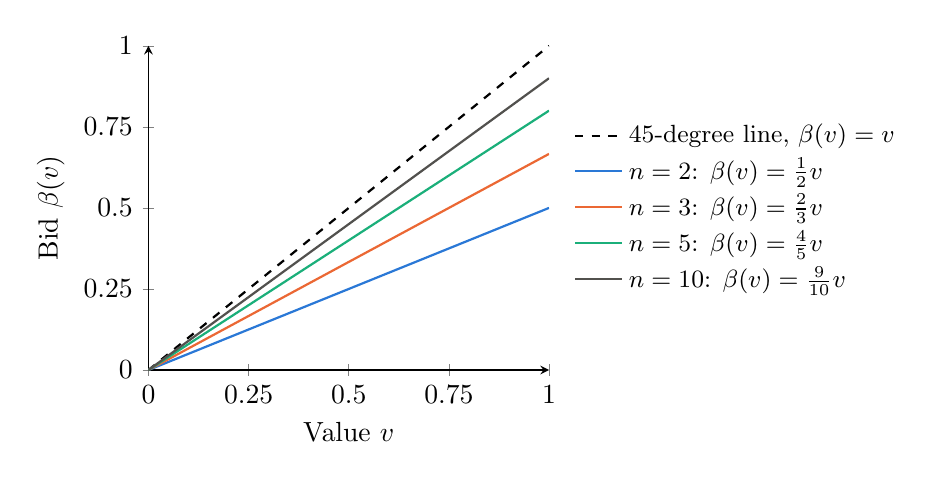
\begin{tikzpicture}
\begin{axis}[width=0.55\textwidth,height=0.47\textwidth,xmin=0,xmax=1,ymin=0,ymax=1,
  xlabel={Value $v$},ylabel={Bid $\beta(v)$},axis lines=left,
  xtick={0,0.25,0.5,0.75,1},ytick={0,0.25,0.5,0.75,1},
  legend style={at={(1.04,0.5)},anchor=west,draw=none,fill=white,font=\small},legend cell align=left]
\addplot[thick,black,dashed,domain=0:1] {x};
\addlegendentry{45-degree line, $\beta(v)=v$}
\addplot[thick,c14blue,domain=0:1] {x/2};
\addlegendentry{$n=2$: $\beta(v)=\frac{1}{2}v$}
\addplot[thick,c14orange,domain=0:1] {2*x/3};
\addlegendentry{$n=3$: $\beta(v)=\frac{2}{3}v$}
\addplot[thick,c14aqua,domain=0:1] {4*x/5};
\addlegendentry{$n=5$: $\beta(v)=\frac{4}{5}v$}
\addplot[thick,c14gray,domain=0:1] {9*x/10};
\addlegendentry{$n=10$: $\beta(v)=\frac{9}{10}v$}
\end{axis}
\end{tikzpicture}
\caption{Equilibrium bids in the first-price auction with values uniform on $[0,1]$ and no reserve price, $\beta(v)=\frac{n-1}{n}v$. Shading falls as the number of bidders grows.}\label{fig:14-rs-uniform}
\end{figure}

\begin{example}[Uniform values with a reserve price]\label{ex:14-uniform-reserve}
Keep $F(v)=v$ on $[0,1]$ and let $r\in(0,1)$. Then
\[
\int_r^v t^{n-1}\,dt=\frac{v^n-r^n}{n},
\]
and \eqref{eq:14-rs-bid} gives, for $v\ge r$,
\[
\beta(v)=v-\frac{v^n-r^n}{nv^{n-1}}=\frac{n-1}{n}\,v+\frac{r^n}{n\,v^{n-1}}.
\]
The reserve raises the bid of every participant by $\frac{r^n}{nv^{n-1}}$. For $n=2$ and $r=\frac12$,
\[
\beta(v)=\frac{v}{2}+\frac{1}{8v},\qquad v\in\Big[\frac12,1\Big],
\]
so that $\beta(\frac12)=\frac12$ and $\beta(1)=\frac58$. The object is sold when the highest value $V_{(2:2)}$, with density $2v$, is at least $\frac12$. Expected revenue is
\[
\int_{\frac{1}{2}}^{1}\Big(\frac{v}{2}+\frac{1}{8v}\Big)2v\,dv=\int_{\frac{1}{2}}^{1}\Big(v^2+\frac14\Big)dv=\Big[\frac{v^3}{3}+\frac{v}{4}\Big]_{\frac{1}{2}}^{1}=\frac{7}{12}-\frac{1}{6}=\frac{5}{12}.
\]
The reserve price raises expected revenue from $\frac13$ to $\frac{5}{12}$. \Cref{sec:14-optimal} shows that $r=\frac12$ is the revenue-maximizing reserve for these values.
\end{example}

\begin{figure}[htbp]
\centering
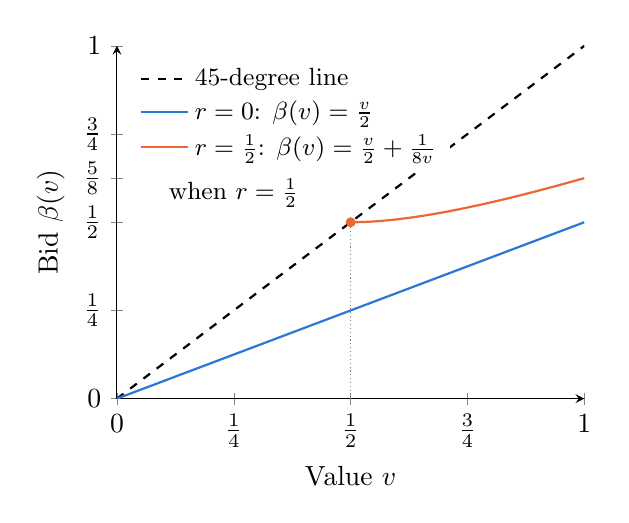
\begin{tikzpicture}
\begin{axis}[width=0.62\textwidth,height=0.5\textwidth,xmin=0,xmax=1,ymin=0,ymax=1,
  xlabel={Value $v$},ylabel={Bid $\beta(v)$},axis lines=left,
  xtick={0,0.25,0.5,0.75,1},xticklabels={$0$,$\frac14$,$\frac12$,$\frac34$,$1$},
  ytick={0,0.25,0.5,0.625,0.75,1},yticklabels={$0$,$\frac14$,$\frac12$,$\frac58$,$\frac34$,$1$},
  legend style={at={(0.03,0.97)},anchor=north west,draw=none,fill=white,font=\small},legend cell align=left]
\addplot[thick,black,dashed,domain=0:1] {x};
\addlegendentry{45-degree line}
\addplot[thick,c14blue,domain=0:1] {x/2};
\addlegendentry{$r=0$: $\beta(v)=\frac{v}{2}$}
\addplot[thick,c14orange,domain=0.5:1,samples=60] {x/2+1/(8*x)};
\addlegendentry{$r=\frac12$: $\beta(v)=\frac{v}{2}+\frac{1}{8v}$}
\addplot[only marks,mark=*,c14orange,mark size=1.6pt] coordinates {(0.5,0.5)};
\draw[densely dotted,gray] (axis cs:0.5,0) -- (axis cs:0.5,0.5);
\node[font=\small,align=center] at (axis cs:0.25,0.62) {no bid\\when $r=\frac12$};
\end{axis}
\end{tikzpicture}
\caption{Equilibrium bids with two bidders and values uniform on $[0,1]$, without a reserve price and with $r=\frac12$. Values below the reserve do not bid. Participants bid more than without a reserve, and the bid function is flat at $v=r$.}\label{fig:14-rs-reserve}
\end{figure}

\begin{example}[Power distribution]\label{ex:14-power}
Let $F(v)=v^\gamma$ on $[0,1]$ with $\gamma>0$, and $r=0$. Then $F(t)^{n-1}=t^{\gamma(n-1)}$ and
\[
\int_0^v t^{\gamma(n-1)}\,dt=\frac{v^{\gamma(n-1)+1}}{\gamma(n-1)+1}.
\]
Substituting into \eqref{eq:14-rs-bid} gives
\[
\beta(v)=v-\frac{v^{\gamma(n-1)+1}}{\big(\gamma(n-1)+1\big)v^{\gamma(n-1)}}=v-\frac{v}{\gamma(n-1)+1}=\frac{\gamma(n-1)}{\gamma(n-1)+1}\,v.
\]
The parameters enter only through the product $\gamma(n-1)$. The reason is that bidding depends on $F$ and $n$ only through the distribution of the highest rival value, $F_{Y_1}(y)=y^{\gamma(n-1)}$. A bidder facing $n-1$ rivals with exponent $\gamma$ bids like a bidder facing one rival with exponent $\gamma(n-1)$. A larger $\gamma$ shifts probability toward high values, which stiffens competition and reduces shading.
\end{example}

\begin{example}[Exponential values, two bidders]\label{ex:14-exponential}
Let $F(v)=1-e^{-\lambda v}$ on $[0,\infty)$ with $\lambda>0$, $n=2$ and $r=0$. Then
\[
\int_0^v\big(1-e^{-\lambda t}\big)dt=v-\frac{1-e^{-\lambda v}}{\lambda}.
\]
Substituting into \eqref{eq:14-rs-bid} gives
\[
\beta(v)=v-\frac{v-\frac{1-e^{-\lambda v}}{\lambda}}{1-e^{-\lambda v}}=v-\frac{v}{1-e^{-\lambda v}}+\frac{1}{\lambda}=\frac{1}{\lambda}-\frac{v\,e^{-\lambda v}}{1-e^{-\lambda v}}.
\]
The last term equals $\frac{v}{e^{\lambda v}-1}$. It tends to $\frac{1}{\lambda}$ as $v\to 0$ and to $0$ as $v\to\infty$. Hence $\beta(0)=0$ and $\beta(v)$ rises toward $\frac{1}{\lambda}=\E[V]$. Values are unbounded, yet no bid exceeds the mean value. Form \eqref{eq:14-rs-condexp} explains why: with two bidders, $\beta(v)=\E[V_j\mid V_j<v]$, which is below $\E[V_j]$. Expected revenue equals $\frac{1}{2\lambda}$, the mean of the lower of two independent exponential values.
\end{example}

The examples suggest that bids rise with the number of bidders. The next result confirms this for every distribution.

\begin{proposition}[More bidders, less shading]\label{prop:14-fpa-n}
Let \cref{ass:14-sipv} hold and fix $r$. For every $v>r$, the shading $v-\beta(v)$ strictly decreases in $n$ and converges to zero as $n\to\infty$. Equilibrium bids therefore rise with $n$ and converge to values.
\end{proposition}

\begin{proof}
By \eqref{eq:14-rs-bid}, the shading of type $v$ is
\[
v-\beta(v)=\int_r^v\Big(\frac{F(t)}{F(v)}\Big)^{n-1}dt.
\]
The density is positive on $(\underline v,\bar v)$, so $F$ is strictly increasing there and $0\le\frac{F(t)}{F(v)}<1$ for $t<v$. The integrand therefore decreases in $n$ at every $t<v$, strictly wherever $F(t)>0$. This set of $t$ has positive length in $[r,v]$, so the integral strictly decreases in $n$. As $n\to\infty$ the integrand converges to zero at every $t<v$. It is bounded by one on the bounded interval $[r,v]$, so the dominated convergence theorem gives convergence of the integral to zero.
\end{proof}

Conditional on winning, a bidder's estimate of the second-highest value rises with the number of rivals. More bidders thus discipline markdowns in the way that more Cournot competitors discipline markups (\cref{ch:theory}).

\Cref{tab:14-uniform-formats} collects the uniform-value equilibria of six auction formats. The all-pay and third-price bids are derived in \cref{sec:14-ret}. Every format yields expected revenue $\frac{n-1}{n+1}$, and every type makes the same expected payment in every format. This regularity motivates \cref{sec:14-ret}.

\begin{table}[htbp]
\centering
\begin{threeparttable}
\caption{Equilibrium bids, expected payments and expected revenue in six formats, with $n$ symmetric bidders, values uniform on $[0,1]$, and no reserve price.}\label{tab:14-uniform-formats}
\small
\begin{tabular}{lccc}
\toprule
Format & Bid of type $v$ & Expected payment of type $v$ & Expected revenue\\
\midrule
First-price sealed bid & $\frac{n-1}{n}v$ & $\frac{n-1}{n}v^n$ & $\frac{n-1}{n+1}$\\[3pt]
Dutch (descending clock) & stop at $\frac{n-1}{n}v$ & $\frac{n-1}{n}v^n$ & $\frac{n-1}{n+1}$\\[3pt]
Second-price sealed bid & $v$ & $\frac{n-1}{n}v^n$ & $\frac{n-1}{n+1}$\\[3pt]
English (button) & exit at $v$ & $\frac{n-1}{n}v^n$ & $\frac{n-1}{n+1}$\\[3pt]
All-pay & $\frac{n-1}{n}v^n$ & $\frac{n-1}{n}v^n$ & $\frac{n-1}{n+1}$\\[3pt]
Third-price ($n\ge 3$) & $\frac{n-1}{n-2}v$ & $\frac{n-1}{n}v^n$ & $\frac{n-1}{n+1}$\\
\bottomrule
\end{tabular}
\begin{tablenotes}
\footnotesize
\item Notes: The expected payment of type $v$ is taken before the outcome is known, so it includes the event of losing. In the first-price and Dutch auctions it equals the bid times the win probability $v^{n-1}$. In the second-price and English auctions it equals $\E[Y_1\indic(Y_1<v)]=\int_0^v y\,(n-1)y^{n-2}dy$. In the all-pay auction it equals the bid. Expected revenue is $n\int_0^1\frac{n-1}{n}v^n\,dv$.
\end{tablenotes}
\end{threeparttable}
\end{table}

\subsection{The first-order condition in terms of the bid distribution}\label{sec:14-fpa-G}

The equilibrium can be characterized without reference to $F$ or $\beta$. Let $G$ denote the distribution function of a single rival's equilibrium bid and $g$ its density, and suppose the reserve price does not bind ($r=\underline v$). In the symmetric equilibrium, $G(b)=\Pr\big(\beta(V_j)\le b\big)=F\big(\beta^{-1}(b)\big)$ on the bid support $[\underline b,\bar b]=[\beta(\underline v),\beta(\bar v)]$. A bidder with value $v_i$ takes $G$ as given and solves
\[
\max_b\;(v_i-b)\,G(b)^{n-1}.
\]
The first-order condition is
\[
-G(b)^{n-1}+(v_i-b)(n-1)G(b)^{n-2}g(b)=0.
\]
Dividing by $(n-1)G(b)^{n-2}g(b)$ and solving for $v_i$ gives
\begin{equation}\label{eq:14-foc-G}
v_i=b+\frac{G(b)}{(n-1)\,g(b)}.
\end{equation}

Equation \eqref{eq:14-foc-G} is the differential equation \eqref{eq:14-rs-ode} written in terms of the bid distribution. To see this, differentiate $G(b)=F(\beta^{-1}(b))$ to get $g(b)=\frac{f(\beta^{-1}(b))}{\beta'(\beta^{-1}(b))}$. At $b=\beta(v)$,
\[
\frac{G(b)}{(n-1)g(b)}=\frac{F(v)\,\beta'(v)}{(n-1)f(v)}=v-\beta(v),
\]
where the last equality is \eqref{eq:14-rs-ode}. For uniform values, $\beta(v)=\frac{n-1}{n}v$, so bids lie in $[0,\frac{n-1}{n}]$ with $G(b)=\frac{nb}{n-1}$ and $g(b)=\frac{n}{n-1}$. Then $\frac{G(b)}{(n-1)g(b)}=\frac{b}{n-1}$, and \eqref{eq:14-foc-G} gives $v=\frac{nb}{n-1}$, which inverts the bid function.

The right side of \eqref{eq:14-foc-G} involves only the bid, the bid distribution, and the number of bidders. All three are observable when bids are recorded. Each bid can therefore be mapped into the value that rationalizes it, without solving a differential equation and without knowing $F$. \Citet{GuerrePerrigneVuong2000} build their identification result and their two-step nonparametric estimator on this observation (\cref{ch:auction-empirics}). In equilibrium the map $b\mapsto b+\frac{G(b)}{(n-1)g(b)}$ equals $\beta^{-1}$, so it must be strictly increasing. This is a testable restriction on bid data.

The condition also has an economic reading. Rewrite \eqref{eq:14-foc-G} as a markdown relative to the bid:
\begin{equation}\label{eq:14-markdown}
\frac{v_i-b}{b}=\frac{1}{\eta(b)},\qquad \eta(b)=(n-1)\frac{b\,g(b)}{G(b)}=\frac{d\ln G(b)^{n-1}}{d\ln b}.
\end{equation}
Here $\eta(b)$ is the elasticity of the win probability $G(b)^{n-1}$ with respect to the bid. \Citet[footnote 13]{AtheyHaile2007} compare this markdown to that of an \emph{oligopsonist}, a buyer that sets its price from the equilibrium elasticity of its residual supply curve. In the auction, the distribution of the highest rival bid plays the role of the residual supply curve. A buyer that values one unit at $v$ and faces residual supply $S(w)$ maximizes $(v-w)S(w)$, which gives $\frac{v-w}{w}=\frac{1}{\varepsilon_S}$ with $\varepsilon_S$ the supply elasticity. With a single rival the bidder is a monopsonist facing that rival's bid distribution, which is our own reading of the analogy. The markdown rule is the buyer's mirror image of the Lerner rule $\frac{p-c}{p}=\frac{1}{\varepsilon}$ (\cref{ch:theory}). Recovering a value from a bid mirrors recovering marginal cost from a pricing first-order condition (\cref{ch:diffprod}). For uniform values $\eta(b)=n-1$ at every bid, so the relative markdown is $\frac{1}{n-1}$. \Cref{sec:14-procurement} develops the same analogy for procurement auctions, where the bid is a price and the win probability a quantity.

Integrating \eqref{eq:14-foc-G} over the bid distribution yields a simple relation between mean values and mean bids \citep[Section 2.2.1]{AtheyHaile2007}.

\begin{proposition}[Mean values and mean bids]\label{prop:14-mean-bid}
In the symmetric equilibrium of the first-price auction under \cref{ass:14-sipv} with a nonbinding reserve price, let $B$ denote an equilibrium bid, with support $[\underline b,\bar b]$. Then
\begin{equation}\label{eq:14-mean-bid}
\E[V]=\frac{n-2}{n-1}\,\E[B]+\frac{1}{n-1}\,\bar b,\qquad \E[V-B]=\frac{1}{n-1}\big(\bar b-\E[B]\big).
\end{equation}
\end{proposition}

\begin{proof}
In equilibrium $V=B+\frac{G(B)}{(n-1)g(B)}$, where $B$ has density $g$. Taking expectations,
\[
\E[V]=\E[B]+\frac{1}{n-1}\int_{\underline b}^{\bar b}\frac{G(b)}{g(b)}\,g(b)\,db=\E[B]+\frac{1}{n-1}\int_{\underline b}^{\bar b}G(b)\,db.
\]
Integration by parts with $G(\underline b)=0$ and $G(\bar b)=1$ gives
\[
\int_{\underline b}^{\bar b}G(b)\,db=\Big[b\,G(b)\Big]_{\underline b}^{\bar b}-\int_{\underline b}^{\bar b}b\,g(b)\,db=\bar b-\E[B].
\]
Substituting,
\[
\E[V]=\E[B]+\frac{\bar b-\E[B]}{n-1}=\frac{n-2}{n-1}\E[B]+\frac{1}{n-1}\bar b.
\]
The second equation in \eqref{eq:14-mean-bid} follows by subtracting $\E[B]$.
\end{proof}

With two bidders the relation reduces to $\E[V]=\bar b$: the highest bid in the support equals the mean value. Form \eqref{eq:14-rs-condexp} gives the same result directly, since $\beta(\bar v)=\E[Y_1\mid Y_1<\bar v]=\E[V]$ when $n=2$. For uniform values with $n$ bidders, $\E[B]=\frac{n-1}{2n}$ and $\bar b=\frac{n-1}{n}$, and \eqref{eq:14-mean-bid} returns $\frac{n-2}{2n}+\frac{1}{n}=\frac12=\E[V]$. \Citet[Section 2.2.1]{AtheyHaile2007} observe that such moment relations had not been exploited in econometric work.

\subsection{Reserve prices, the Dutch auction, and multiplicity}\label{sec:14-fpa-multiplicity}

The Dutch auction is strategically equivalent to the first-price auction (\cref{prop:14-dutch-fpa}). Its equilibrium is therefore the same: a bidder with value $v\ge r$ stops the descending clock at the price $\beta(v)$ given by \eqref{eq:14-rs-bid}.

A reserve price has two effects in the first-price auction. It excludes all values below $r$, and it raises the bids of all participants. Write $\beta_r$ for the equilibrium bid with reserve $r$ and $\beta_{\underline v}$ for the bid without a binding reserve. By \eqref{eq:14-rs-bid}, for $v>r$,
\[
\beta_r(v)-\beta_{\underline v}(v)=\frac{\int_{\underline v}^v F(t)^{n-1}dt-\int_r^v F(t)^{n-1}dt}{F(v)^{n-1}}=\frac{\int_{\underline v}^r F(t)^{n-1}\,dt}{F(v)^{n-1}}>0.
\]
The reserve acts like an extra competitor who bids $r$. With uniform values the increase is $\frac{r^n}{nv^{n-1}}$, as in \cref{ex:14-uniform-reserve}. The effect fades as $v$ rises, because a high-value bidder rarely faces a situation in which the reserve is the binding competitor. The net effect on revenue weighs the higher bids against the lost sales, and \cref{sec:14-optimal} resolves it.

The boundary condition $\beta(r)=r$ in \cref{prop:14-rs} came from the floor on bids. \Citet[footnote 25]{MilgromWeber1982} show that the floor matters. Suppose any real number is a valid bid, including a negative one, which would oblige the seller to pay the winner. Step 1 of the proof then fails. Integrating the differential equation without a boundary condition gives
\[
\beta(v)F(v)^{n-1}=\int_{\underline v}^v t\,d\big[F(t)^{n-1}\big]-k
\]
for an arbitrary constant $k$. Hence the family of candidates is
\begin{equation}\label{eq:14-multiplicity}
\beta_k(v)=\beta(v)-\frac{k}{F(v)^{n-1}},
\end{equation}
where $\beta$ is the bid \eqref{eq:14-rs-bid} with $r=\underline v$. With uniform values on $[0,1]$ this family is
\[
\beta_k(v)=\frac{n-1}{n}\,v-\frac{k}{v^{n-1}},\qquad k\ge 0.
\]
\Citet[footnote 25]{MilgromWeber1982} print the slope of this family as $\frac{n}{n+1}$. That is a misprint. The footnote carries it into the ranges of the strategies, which it prints as $\big(0,\frac{n}{n+1}\big)$ for $k=0$ and $\big(-\infty,\frac{n}{n+1}-k\big)$ for $k>0$. The slope $\frac{n}{n+1}$ violates the first-order condition, since the two sides of \eqref{eq:14-rs-ode} then differ by $\frac{v^{n-1}}{n+1}$, or by $\frac{1}{n+1}$ after dividing by $v^{n-1}$. The slope $\frac{n-1}{n}$ satisfies it and reproduces exactly the ex ante payoff $\frac{1}{n(n+1)}+k$ that the footnote reports, as we now verify.

Fix $k\ge 0$ and suppose all rivals use $\beta_k$. Its derivative is $\beta_k'(v)=\frac{n-1}{n}+\frac{(n-1)k}{v^n}>0$, so $\beta_k$ is strictly increasing. For $k>0$ its range is $\big(-\infty,\frac{n-1}{n}-k\big)$, and for $k=0$ it is $\big(0,\frac{n-1}{n}\big)$. A bid $\beta_k(z)$ wins with probability $z^{n-1}$, so a bidder with value $v$ who mimics type $z$ earns
\[
\Pi_k(z;v)=\big(v-\beta_k(z)\big)z^{n-1}=v\,z^{n-1}-\frac{n-1}{n}z^n+k.
\]
Differentiating with respect to $z$,
\[
\frac{\partial\Pi_k(z;v)}{\partial z}=(n-1)z^{n-2}v-(n-1)z^{n-1}=(n-1)z^{n-2}(v-z).
\]
The payoff peaks at $z=v$. A bid above the range wins for sure at a higher cost than the top of the range, and a bid below the range (possible only when $k=0$) never wins. Hence $\beta_k$ is a symmetric equilibrium for every $k\ge 0$. Type $v$ earns $\Pi_k(v;v)=\frac{v^n}{n}+k$, and the ex ante payoff is
\[
\int_0^1\Big(\frac{v^n}{n}+k\Big)dv=\frac{1}{n(n+1)}+k.
\]
The allocation is efficient in every member of the family, so total surplus is the same. Each bidder gains $k$, and the seller's expected revenue falls to $\frac{n-1}{n+1}-nk$. In the equilibria with $k>0$, low types submit large negative bids, and even a bidder with value zero expects to receive $k$. \Citet[footnote 25]{MilgromWeber1982} suggest that this possibility may explain why almost all observed auctions have at least an implicit reserve price. The lesson is that the floor on bids, set by a reserve price or by a nonnegativity rule, selects the equilibrium. In empirical work the floor is part of the rules and should be recorded with the bids.

\subsection{Risk-averse bidders}\label{sec:14-fpa-risk}

We now replace risk neutrality in \cref{ass:14-sipv}(i). Each bidder has a utility of money $\mathcal U$ that is strictly increasing and concave, with $\mathcal U(0)=0$, and twice differentiable on $(0,\infty)$. A bidder with value $v$ who wins at price $b$ receives $\mathcal U(v-b)$, and a losing bidder receives $\mathcal U(0)=0$. We look for a symmetric equilibrium with strictly increasing bid function $\beta_u$ and bid distribution $G$.

A bidder with value $v$ solves
\[
\max_b\;\mathcal U(v-b)\,G(b)^{n-1}.
\]
The first-order condition is
\[
-\mathcal U'(v-b)\,G(b)^{n-1}+\mathcal U(v-b)(n-1)G(b)^{n-2}g(b)=0,
\]
which simplifies, after division by $G(b)^{n-2}$, to
\[
\mathcal U'(v-b)\,G(b)=(n-1)\,\mathcal U(v-b)\,g(b).
\]
Following \citet[eq.~(6.24)]{AtheyHaile2007}, define the ratio
\begin{equation}\label{eq:14-ell}
\ell(s)=\frac{\mathcal U(s)}{\mathcal U'(s)}.
\end{equation}
They denote this ratio by $\lambda$. We write $\ell$ to keep $\lambda$ for the exponential rate of \cref{ex:14-exponential}. The first-order condition becomes $\ell(v-b)=\frac{G(b)}{(n-1)g(b)}$, so
\begin{equation}\label{eq:14-risk-foc}
v=b+\ell^{-1}\Big(\frac{G(b)}{(n-1)\,g(b)}\Big),
\end{equation}
which is their eq.~(6.25). The ratio has three properties. First, $\ell(0)=\lim_{s\downarrow 0}\ell(s)=0$. Second, $\ell'(s)=1-\frac{\mathcal U(s)\,\mathcal U''(s)}{\mathcal U'(s)^2}\ge 1$, so $\ell$ is strictly increasing and invertible. Third, concavity and $\mathcal U(0)=0$ give $0=\mathcal U(0)\le\mathcal U(s)+\mathcal U'(s)(0-s)$, that is,
\[
\ell(s)\ge s\quad\text{for } s\ge 0,
\]
with strict inequality for $s>0$ when $\mathcal U$ is strictly concave. Under risk neutrality $\ell(s)=s$, and \eqref{eq:14-risk-foc} reduces to \eqref{eq:14-foc-G}.

In terms of the bid function, $G(b)=F(\beta_u^{-1}(b))$, so at $b=\beta_u(v)$ we have $\frac{G(b)}{(n-1)g(b)}=\frac{F(v)\beta_u'(v)}{(n-1)f(v)}$. Substituting into $\ell(v-b)=\frac{G(b)}{(n-1)g(b)}$ and solving for $\beta_u'(v)$,
\begin{equation}\label{eq:14-risk-ode}
\beta_u'(v)=\frac{\mathcal U\big(v-\beta_u(v)\big)}{\mathcal U'\big(v-\beta_u(v)\big)}\,\frac{f_{Y_1}(v)}{F_{Y_1}(v)}\;\ge\;\big(v-\beta_u(v)\big)\frac{f_{Y_1}(v)}{F_{Y_1}(v)},
\end{equation}
where $\frac{f_{Y_1}}{F_{Y_1}}=(n-1)\frac{f}{F}$ and the inequality uses $\ell(s)\ge s$. This is eq.~(11) of \citet{MilgromWeber1982}. The boundary condition is again $\beta_u(\underline v)=\underline v$, by the argument of Step 1 of \cref{prop:14-rs}.

\begin{example}[Constant relative risk aversion]\label{ex:14-crra}
Let $\mathcal U(x)=x^a$ with $0<a\le 1$, a case of constant relative risk aversion (CRRA), so that the coefficient of relative risk aversion is $1-a$. Then $\ell(s)=\frac{s^a}{a s^{a-1}}=\frac{s}{a}$. Let values be uniform on $[0,1]$, so $\frac{f_{Y_1}(v)}{F_{Y_1}(v)}=\frac{n-1}{v}$. Equation \eqref{eq:14-risk-ode} becomes
\[
\beta_u'(v)=\frac{(n-1)\big(v-\beta_u(v)\big)}{a\,v},
\]
a linear differential equation:
\[
\beta_u'(v)+\frac{n-1}{a\,v}\,\beta_u(v)=\frac{n-1}{a}.
\]
We try $\beta_u(v)=cv$. Substituting gives $c+\frac{(n-1)c}{a}=\frac{n-1}{a}$, so $c(a+n-1)=n-1$. The homogeneous equation adds solutions $Cv^{-\frac{n-1}{a}}$, which are unbounded near zero, and the boundary condition $\beta_u(0)=0$ forces $C=0$. Hence
\[
\beta_u(v)=\frac{n-1}{n-1+a}\,v.
\]
With $a=1$ we recover $\frac{n-1}{n}v$. As $a$ falls, bids rise, and they approach values as $a\to 0$. Expected revenue is $\frac{n-1}{n-1+a}\cdot\frac{n}{n+1}$. Its ratio to the second-price revenue $\frac{n-1}{n+1}$ is $\frac{n}{n-1+a}$, which exceeds one whenever $a<1$. For example, with $n=2$ and $a=\frac12$, bids are $\frac23v$ and expected revenue is $\frac49$, against $\frac13$ in the second-price auction.
\end{example}

The example ranks the formats. To prove the ranking in general we need a simple comparison lemma, which \cref{sec:14-mw-rank} also uses.

\begin{lemma}[Crossing lemma, \citealp{MilgromWeber1982}, Lemma 2]\label{lem:14-crossing}
Let $h_1$ and $h_2$ be continuous on $[\underline x,\bar x]$ and differentiable on $(\underline x,\bar x]$. Suppose (i) $h_1(\underline x)\ge h_2(\underline x)$, and (ii) $h_1(x)<h_2(x)$ implies $h_1'(x)\ge h_2'(x)$. Then $h_1(x)\ge h_2(x)$ for all $x\in[\underline x,\bar x]$.
\end{lemma}

\begin{proof}
Let $d=h_1-h_2$ and suppose, to the contrary, that $d(x)<0$ for some $x>\underline x$. The set $\{t\in[\underline x,x]:d(t)\ge 0\}$ is closed and contains $\underline x$. Let $x_0$ be its largest element. Then $d(x_0)\ge 0$, $x_0<x$, and $d<0$ on $(x_0,x]$. By the mean value theorem there is $\hat x\in(x_0,x)$ with
\[
d'(\hat x)=\frac{d(x)-d(x_0)}{x-x_0}<0.
\]
At $\hat x$ we have $h_1(\hat x)<h_2(\hat x)$ and $h_1'(\hat x)<h_2'(\hat x)$, which contradicts (ii).
\end{proof}

\begin{proposition}[Risk aversion favors the first-price auction, \citealp{Holt1980,MaskinRiley1984}]\label{prop:14-risk-fpa}
Let \cref{ass:14-sipv} hold with risk neutrality replaced by a common utility $\mathcal U$ that is strictly increasing and concave, with $\mathcal U(0)=0$, and twice differentiable on $(0,\infty)$. Let there be no binding reserve price. Then the first-price auction yields at least as much expected revenue as the second-price auction. The ranking is strict when $\mathcal U$ is strictly concave.
\end{proposition}

\begin{proof}
\emph{Step 1.} We start with the second-price auction. Bidding one's value remains a weakly dominant strategy. The proof of \cref{prop:14-spa-dominant} compares the surplus $v-m$ from winning at the highest rival bid $m$ with zero, and an increasing $\mathcal U$ preserves its sign. Expected revenue is therefore $\E[V_{(n-1:n)}]$, as with risk neutrality. Let $\beta_N$ be the risk-neutral first-price bid. By \eqref{eq:14-rs-condexp} with $r=\underline v$, $\beta_N(v)=\E[Y_1\mid Y_1<v]$. Conditional on $V_{(n:n)}=v$, the second-highest value is distributed as $Y_1$ given $Y_1<v$. The law of iterated expectations therefore gives $\E[V_{(n-1:n)}]=\E[\beta_N(V_{(n:n)})]$.

\emph{Step 2.} We show that risk-averse bidders bid more. The risk-neutral bid satisfies $\beta_N'(v)=\big(v-\beta_N(v)\big)\frac{f_{Y_1}(v)}{F_{Y_1}(v)}$. We apply \cref{lem:14-crossing} with $h_1=\beta_u$ and $h_2=\beta_N$. Condition (i) holds because $\beta_u(\underline v)=\beta_N(\underline v)=\underline v$. For condition (ii), suppose $\beta_u(v)<\beta_N(v)$. Then \eqref{eq:14-risk-ode} gives
\[
\beta_u'(v)\ge\big(v-\beta_u(v)\big)\frac{f_{Y_1}(v)}{F_{Y_1}(v)}>\big(v-\beta_N(v)\big)\frac{f_{Y_1}(v)}{F_{Y_1}(v)}=\beta_N'(v).
\]
The lemma yields $\beta_u(v)\ge\beta_N(v)$ for all $v$.

\emph{Step 3.} We compare revenues. Both bid functions are strictly increasing, so the bidder with the highest value wins in both cases. Expected first-price revenue with risk aversion is $\E[\beta_u(V_{(n:n)})]\ge\E[\beta_N(V_{(n:n)})]$, which is the second-price revenue by Step 1.

\emph{Step 4.} We prove strictness. If $\mathcal U$ is strictly concave, then $\ell(s)>s$ for $s>0$. Let $d=\beta_u-\beta_N\ge 0$ and suppose $d(v)=0$ at some $v>\underline v$. Then $v-\beta_u(v)=v-\beta_N(v)>0$, and \eqref{eq:14-risk-ode} holds with strict inequality, so $d'(v)>0$. Hence $d<0$ just to the left of $v$, a contradiction. Thus $\beta_u>\beta_N$ on $(\underline v,\bar v]$, and the revenue ranking is strict.
\end{proof}

The intuition is that shading is a gamble. A lower bid raises the gain from winning but lowers the chance of winning. A risk-averse bidder dislikes this gamble and buys insurance against losing by bidding more. In the second-price auction the bid does not affect the price paid upon winning, so there is no gamble to manage. \Citet[p.~1114]{MilgromWeber1982} combine this result with their ranking for affiliated values. With both affiliation and risk aversion, the first-price and second-price auctions cannot be ranked in general (\cref{sec:14-mw-risk}).

Risk aversion also complicates the inversion of bids. Equation \eqref{eq:14-risk-foc} requires the function $\ell$, which a single bid distribution cannot pin down \citep[Section 6.4]{AtheyHaile2007}. In the CRRA case, $\ell^{-1}(x)=ax$, so values satisfy $V=B+a\frac{G(B)}{(n-1)g(B)}$. Bids rationalized by exponent $a$ are equally well rationalized by any $\tilde a\in(0,a)$ with values
\[
\tilde V=B+\frac{\tilde a}{a}\,(V-B),
\]
which lie between the bids and the original values. More risk-averse bidders with lower values produce the same bids. \Cref{ch:auction-empirics} returns to this identification problem.

Empirical work suggests that the effect is not small. \Citet{CampoEtAl2011} break the indeterminacy with a parametric utility function and a parametric quantile restriction. In sealed-bid timber auctions of the U.S.\ Forest Service, they estimate a CRRA measure of 0.278 \citep[Section~2.4, p.~95]{HortacsuPerrigne2021}. Under CRRA, risk aversion acts like an increase in competition and lowers the bidders' information rents. Exercise~3(b) of \cref{sec:14-exercises} makes this precise. Bidders already bid aggressively, so the seller needs a smaller reserve price. The simulated optimal reserve price is about 19 percent below the one computed under risk neutrality \citep[p.~95]{HortacsuPerrigne2021}.

\casehead{The original papers} \citet{Holt1980} studies procurement auctions with risk-averse bidders and shows that the first-price format yields a lower expected cost to the buyer than the oral or second-price formats. \Citet{MaskinRiley1984} characterize the revenue-maximizing auction when buyers are risk averse. They show that the first-price auction dominates the second-price auction and that the optimal mechanism differs from all the standard formats.
\Citet[p.~1093]{MilgromWeber1982} list the risk-aversion ranking as the seventh conclusion of the independent private values model. They credit it to \citet{HarrisRaviv1981}, \citet{Holt1980}, a 1980 discussion paper by Maskin and Riley, and a 1979 working paper by Matthews. On p.~1114 they give the proof by \cref{lem:14-crossing} that we follow.

\section{Revenue Equivalence}\label{sec:14-ret}

Every format in \cref{tab:14-uniform-formats} yields the same expected revenue. Each type even makes the same expected payment in every format. This section explains the regularity. We first present the geometric argument of \citet{MilgromWeber1982}, then the mechanism-design formulation of \citet{Myerson1981}. We use the theorem to solve for equilibria of new formats, extend it to interdependent values with independent signals, and list the assumptions whose failure breaks it.

\subsection{The self-selection view}\label{sec:14-ret-selfselection}

With independent private values, the four standard formats yield the same expected revenue. \Citet[p.~1092]{MilgromWeber1982} credit this finding to \citet{OrtegaReichert1968} and \citet{Vickrey1962}. They add that it remained a puzzle until the self-selection approach of \citet{HarrisRaviv1981}, \citet{Myerson1981} and \citet{RileySamuelson1981}. We follow their exposition. In this subsection only, $p$ denotes a probability of winning, as in their paper.

Fix the rules of an auction and the strategies of bidder $i$'s rivals. Every action available to bidder $i$, whether a bid, a stopping price or a plan of exits, leads to some probability of winning $p$ and some expected payment. Let $e(p)$ denote the lowest expected payment among the actions that win with probability $p$. Because values are independent, the menu of pairs $(p,e(p))$ depends only on the rules and on the rivals' strategies. It does not depend on bidder $i$'s own value.

A bidder with value $v$ who chooses the pair $(p,e)$ obtains expected utility $vp-e$. Its indifference curves in the $(p,e)$ plane are straight lines $e=vp-\text{constant}$ with slope $v$. A lower intercept means a higher utility. It therefore chooses the point of the menu that touches the lowest line of slope $v$. Let $p^*(v)$ denote the chosen probability. \Cref{fig:14-mw-selfselection} illustrates the choice.

\begin{figure}[htbp]
\centering
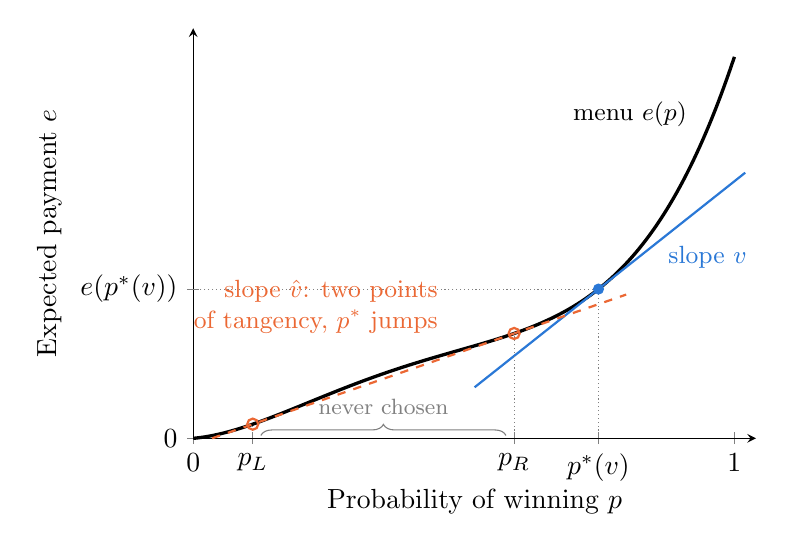
\begin{tikzpicture}
\begin{axis}[width=0.72\textwidth,height=0.56\textwidth,xmin=0,xmax=1.04,ymin=0,ymax=0.86,
  axis lines=left,xlabel={Probability of winning $p$},ylabel={Expected payment $e$},
  xtick={0,0.11013,0.59299,0.74883,1},xticklabels={$0$,$p_L$,$p_R$,$p^*(v)$,$1$},
  ytick={0,0.31300},yticklabels={$0$,$e(p^*(v))$},
  every axis x label/.style={at={(axis description cs:0.5,-0.1)},anchor=north},
  clip=false]
\addplot[very thick,black,domain=0:1,samples=200] {0.1*x+2*x^2-4.5*x^3+3.2*x^4};
\addplot[thick,c14blue,domain=0.52:1.02] {0.9*x-0.36094};
\addplot[thick,c14orange,dashed,domain=0.035:0.8] {0.39388*x-0.01365};
\addplot[only marks,mark=*,c14blue,mark size=1.8pt] coordinates {(0.74883,0.31300)};
\addplot[only marks,mark=o,c14orange,mark size=2pt,thick] coordinates {(0.11013,0.02973) (0.59299,0.21992)};
\draw[densely dotted,gray] (axis cs:0.74883,0) -- (axis cs:0.74883,0.31300) -- (axis cs:0,0.31300);
\draw[densely dotted,gray] (axis cs:0.11013,0) -- (axis cs:0.11013,0.02973);
\draw[densely dotted,gray] (axis cs:0.59299,0) -- (axis cs:0.59299,0.21992);
\node[font=\small,c14blue,anchor=west] at (axis cs:0.86,0.38) {slope $v$};
\node[font=\small,c14orange,anchor=south east,align=right] at (axis cs:0.47,0.20) {slope $\hat v$: two points\\of tangency, $p^*$ jumps};
\node[font=\small,anchor=east] at (axis cs:0.93,0.68) {menu $e(p)$};
\draw[decorate,decoration={brace,amplitude=4pt},gray] (axis cs:0.125,0.006) -- (axis cs:0.578,0.006) node[midway,above=4pt,font=\footnotesize] {never chosen};
\end{axis}
\end{tikzpicture}
\caption{The bidder's choice among pairs of win probability and expected payment. Indifference lines have slope equal to the value. A bidder with value $v$ chooses the point where the lowest line of slope $v$ touches the menu. At the value $\hat v$ the line touches the menu twice, and the chosen win probability jumps from $p_L$ to $p_R$. Redrawn after \citet{MilgromWeber1982}, Figure 1, with an illustrative menu.}\label{fig:14-mw-selfselection}
\end{figure}

Two facts follow from the geometry. First, $p^*$ is nondecreasing. Optimality of $p^*(v)$ for $v$ and of $p^*(v')$ for $v'$ gives two revealed-preference inequalities. Adding them, as in the proof of \cref{lem:14-monotone}, yields $(v'-v)\big[p^*(v')-p^*(v)\big]\ge 0$. Second, where $p^*$ is differentiable, the line of slope $v$ is tangent to the menu, so $e'(p^*(v))=v$. The chain rule then gives
\[
\frac{d}{dv}\,e\big(p^*(v)\big)=e'\big(p^*(v)\big)\frac{dp^*(v)}{dv}=v\,\frac{dp^*(v)}{dv}.
\]
Where the line touches the menu at two points, a small increase in $v$ makes $p^*$ jump by $\Delta p^*$. Both points lie on the same line of slope $v$, so the payment jumps by $\Delta e=v\,\Delta p^*$. Combining the smooth parts and the jumps, and integrating from the lowest value $\underline v$,
\begin{equation}\label{eq:14-mw-selfselection}
e\big(p^*(v)\big)=e\big(p^*(\underline v)\big)+\int_{\underline v}^{v}t\,dp^*(t).
\end{equation}

Equation \eqref{eq:14-mw-selfselection} is the core of revenue equivalence. Each type's expected payment depends on the rules only through two objects: the function $p^*$ and the payment of the lowest type. The seller's expected revenue is the sum of the bidders' expected payments, so the same is true of revenue. Every auction that always awards the object to the highest value has $p^*(v)=F(v)^{n-1}$. If, in addition, the lowest type pays nothing, all such auctions produce the same expected revenue. The menu need not be smooth or even continuous \citep[footnote 12]{MilgromWeber1982}. It always contains a point $(0,e(0))$ with $e(0)\le 0$, because a bidder can abstain. The payment $e(0)$ is negative only if the seller subsidizes losing bidders.

For uniform values and two bidders, the first-price menu is easy to compute. A bid $b\in[0,\frac12]$ wins against a rival who bids half its value with probability $p=2b$. The expected payment is $e=bp=\frac{p^2}{2}$. Tangency requires $e'(p)=p=v$, so $p^*(v)=v=F(v)$, and the expected payment is $\frac{v^2}{2}=\int_0^v t\,dt$, as \eqref{eq:14-mw-selfselection} predicts.

\subsection{Mechanisms and incentive compatibility}\label{sec:14-ret-mechanisms}

The general formulation allows asymmetric bidders and arbitrary selling procedures. We use it here and in \cref{sec:14-optimal}.

\begin{assumption}[Independent private values]\label{ass:14-ipv}
There are $n$ risk-neutral bidders. Bidder $i$'s value $V_i$ is drawn from a distribution $F_i$ with a finite mean, support $[\underline v_i,\bar v_i]$ with $\underline v_i$ finite and $\bar v_i\le\infty$, and a density $f_i$ that is strictly positive on the support. Values are independent across bidders. The seller's own value for the object is $v_0$, and it is risk neutral.
\end{assumption}

The seller's value $v_0$ is what the object is worth to the seller if it is not sold. It is not a reserve price.

A \emph{direct mechanism} asks each bidder to report a value. It consists of an allocation rule and a payment rule. The allocation rule $q_i(\bm v)\in[0,1]$ is the probability that bidder $i$ receives the object when the reports are $\bm v=(v_1,\dots,v_n)$, with $\sum_i q_i(\bm v)\le 1$. The payment rule $\tau_i(\bm v)$ is the amount bidder $i$ pays. Bidder $i$ cares about the \emph{interim} allocation and payment, which average over the rivals' values:
\[
Q_i(v_i)=\E\big[q_i(v_i,\bm V_{-i})\big],\qquad m_i(v_i)=\E\big[\tau_i(v_i,\bm V_{-i})\big].
\]
A bidder with value $v_i$ who reports $z$ while the others report truthfully obtains $v_iQ_i(z)-m_i(z)$. Its truthful payoff is
\[
\pi_i(v_i)=v_iQ_i(v_i)-m_i(v_i).
\]
The mechanism is \emph{incentive compatible} (IC) if truth-telling is optimal,
\begin{equation}\label{eq:14-ic}
\pi_i(v_i)\ge v_iQ_i(z)-m_i(z)\quad\text{for all }i,\ v_i,\ z,
\end{equation}
and \emph{individually rational} (IR) if participation is voluntary,
\begin{equation}\label{eq:14-ir}
\pi_i(v_i)\ge 0\quad\text{for all }i,\ v_i.
\end{equation}

The \emph{revelation principle} \citep{Myerson1981} makes direct mechanisms a general tool. Take any auction and any Bayesian Nash equilibrium $(\beta_1,\dots,\beta_n)$ of it. Define $q_i(\bm v)$ and $\tau_i(\bm v)$ as the allocation and payments that result when the bidders play $\beta_1(v_1),\dots,\beta_n(v_n)$. This direct mechanism is incentive compatible. A type $v_i$ who gained by reporting $z$ would have gained in the original auction by playing $\beta_i(z)$, contradicting equilibrium. The direct mechanism produces the same allocation and payments as the auction for every profile of values. Hence any statement about IC direct mechanisms applies to the equilibrium outcomes of all auctions.

\begin{lemma}[Characterization of incentive compatibility]\label{lem:14-ic}
Under \cref{ass:14-ipv}, a direct mechanism is incentive compatible if and only if, for every bidder $i$, (a) $Q_i$ is nondecreasing, and (b) for every $v_i$,
\begin{equation}\label{eq:14-envelope-ic}
\pi_i(v_i)=\pi_i(\underline v_i)+\int_{\underline v_i}^{v_i}Q_i(t)\,dt.
\end{equation}
\end{lemma}

\begin{proof}
We drop the subscript $i$.

\emph{Necessity.} Let $v$ and $v'$ be two values. The IC constraint of type $v$ against report $v'$ reads $\pi(v)\ge vQ(v')-m(v')$. Since $m(v')=v'Q(v')-\pi(v')$, this is
\[
\pi(v)\ge\pi(v')+(v-v')\,Q(v').
\]
Exchanging the roles of $v$ and $v'$ gives
\[
\pi(v')\ge\pi(v)+(v'-v)\,Q(v).
\]
Together the two inequalities give
\[
(v'-v)\,Q(v)\le\pi(v')-\pi(v)\le(v'-v)\,Q(v').
\]
For $v'>v$, dividing by $v'-v$ shows $Q(v)\le Q(v')$, which is (a). Because $0\le Q\le 1$, the same chain gives $|\pi(v')-\pi(v)|\le|v'-v|$. So $\pi$ is Lipschitz, hence absolutely continuous and differentiable almost everywhere. Letting $v'\to v$ in the chain shows that $\pi'(v)=Q(v)$ wherever $Q$ is continuous, which is almost everywhere because $Q$ is monotone. An absolutely continuous function is the integral of its derivative, which gives (b).

\emph{Sufficiency.} Suppose (a) and (b) hold. For any $v$ and $z$, using $m(z)=zQ(z)-\pi(z)$ and (b),
\[
\pi(v)-\big[vQ(z)-m(z)\big]=\pi(v)-\pi(z)-(v-z)Q(z)=\int_z^v\big[Q(t)-Q(z)\big]dt.
\]
If $z<v$, the integrand is nonnegative on $[z,v]$ by (a). If $z>v$, the integral equals $\int_v^z\big[Q(z)-Q(t)\big]dt$, which is also nonnegative by (a). Hence truth-telling is optimal.
\end{proof}

Condition (b) is the envelope formula of \cref{sec:14-fpa-envelope} in general form. Since $m_i(v_i)=v_iQ_i(v_i)-\pi_i(v_i)$, it yields the \emph{payment identity}
\begin{equation}\label{eq:14-payment-identity}
m_i(v_i)=v_iQ_i(v_i)-\pi_i(\underline v_i)-\int_{\underline v_i}^{v_i}Q_i(t)\,dt.
\end{equation}
In an incentive compatible mechanism, the interim allocation and the payoff of the lowest type determine every interim payment.

\subsection{The revenue equivalence theorem}\label{sec:14-ret-theorem}

\begin{proposition}[Revenue equivalence, \citealp{Myerson1981,RileySamuelson1981}]\label{prop:14-ret}
Let \cref{ass:14-ipv} hold. Consider two auctions, each with a Bayesian Nash equilibrium. Suppose the two equilibria induce the same interim allocation $Q_i$ for every bidder, and give the lowest type of each bidder the same expected payoff $\pi_i(\underline v_i)$. Then every type of every bidder makes the same expected payment in the two auctions, and the seller's expected revenue is the same. In particular, let bidders be symmetric ($F_i=F$). Then any auction whose equilibrium awards the object to the highest value and charges the lowest type nothing yields expected revenue $\E[V_{(n-1:n)}]$.
\end{proposition}

\begin{proof}
By the revelation principle, each auction with its equilibrium is an incentive compatible direct mechanism. By the payment identity \eqref{eq:14-payment-identity}, each interim payment $m_i(v_i)$ depends only on $Q_i$ and $\pi_i(\underline v_i)$, which the two auctions share. Expected revenue is $\sum_i\E[m_i(V_i)]$, so it is also the same.

For the symmetric case, the highest value wins, so $Q(v)=F(v)^{n-1}=F_{Y_1}(v)$. The lowest type never wins and pays nothing, so $\pi(\underline v)=0$. The payment identity and integration by parts give
\[
m(v)=vF(v)^{n-1}-\int_{\underline v}^vF(t)^{n-1}\,dt=\int_{\underline v}^v y\,dF_{Y_1}(y)=\E\big[Y_1\indic(Y_1<v)\big].
\]
This is the expected payment of type $v$ in the second-price auction. Summing over bidders,
\[
\sum_{i=1}^n\E\big[m(V_i)\big]=\sum_{i=1}^n\E\Big[\max_{j\neq i}V_j\;\indic\Big(V_i>\max_{j\neq i}V_j\Big)\Big]=\E\big[V_{(n-1:n)}\big].
\]
The last equality holds because exactly one bidder has the highest value, and for that bidder the highest rival value is the second-highest value overall.
\end{proof}

\Citet[Theorem 0]{MilgromWeber1982} state the symmetric case as follows. Assume the independent private values model and a noncooperative equilibrium of some auction mechanism. Suppose that in equilibrium the bidder with the highest value is certain to receive the object, and that a bidder with the lowest possible value has an expected payment of zero. Then the seller's expected revenue equals the expected value of the object to the second-highest evaluator. The symmetric equilibria of the English, Dutch, first-price and second-price auctions satisfy these conditions, so all four yield the same expected price. \Cref{prop:14-ret} generalizes Theorem 0 in two directions: bidders may be asymmetric, and the allocation need not be efficient.

\Citet[p.~1093]{MilgromWeber1982} give the theorem an appealing economic reading. Whatever competitive mechanism sets the price, the sale on average takes place at the lowest price at which supply equals demand. The supply is one unit. At a price $p$, demand is the number of bidders with values above $p$. Demand equals one exactly when $p$ lies between $V_{(n-1:n)}$ and $V_{(n:n)}$, and the lowest such price is $V_{(n-1:n)}$. Revenue equivalence thus says that auctions deliver, on average, the competitive price.

\subsection{Using revenue equivalence to solve for equilibria}\label{sec:14-ret-solve}

Revenue equivalence gives a shortcut to equilibrium bids. Suppose a format has a symmetric equilibrium with a strictly increasing bid function, so that the highest value wins, and the lowest type pays nothing. Then \cref{prop:14-ret} fixes the expected payment of every type at $m(v)=\E[Y_1\indic(Y_1<v)]$. Writing $m(v)$ in terms of the format's bid function gives an equation for that function. The shortcut produces a candidate. Its optimality must still be verified, which we do in each case.

\emph{First-price auction.} The winner pays its bid, so $m(v)=\beta(v)F(v)^{n-1}$. Revenue equivalence gives
\[
\beta(v)=\frac{\E[Y_1\indic(Y_1<v)]}{F_{Y_1}(v)}=\E\left[Y_1\given Y_1<v\right],
\]
which is \eqref{eq:14-rs-condexp} without a reserve price. With a reserve price $r$, the allocation is $Q(v)=F(v)^{n-1}\indic(v\ge r)$ and the type $r$ earns zero. The payment identity then gives $m(v)=vF(v)^{n-1}-\int_r^vF(t)^{n-1}dt=\E[\max\{Y_1,r\}\indic(Y_1<v)]$ for $v\ge r$, which again delivers \eqref{eq:14-rs-condexp}. \Cref{prop:14-rs} verified optimality.

\emph{All-pay auction.} Every bidder pays its bid, win or lose. All-pay auctions model lobbying, research races and other contests in which effort is sunk. Here $m(v)=\beta(v)$, so
\[
\beta^{AP}(v)=\E\big[Y_1\indic(Y_1<v)\big]=\int_{\underline v}^v y\,dF_{Y_1}(y).
\]
For uniform values, $\beta^{AP}(v)=\int_0^v y(n-1)y^{n-2}dy=\frac{n-1}{n}v^n$. To verify optimality, note that a bidder with value $v$ who bids $\beta^{AP}(z)$ earns $vz^{n-1}-\frac{n-1}{n}z^n$. Its derivative with respect to $z$ is $(n-1)z^{n-2}(v-z)$, which changes sign from positive to negative at $z=v$.

\emph{Third-price auction.} With $n\ge 3$ bidders, the highest bidder wins and pays the third-highest bid. Let $Y_2$ denote the second-highest rival value. With a strictly increasing $\beta$, the expected payment is $m(v)=\E[\beta(Y_2)\indic(Y_1<v)]$. Revenue equivalence requires, for every $v$,
\[
\int_{\underline v}^v\E\big[\beta(Y_2)\mid Y_1=y\big]f_{Y_1}(y)\,dy=\int_{\underline v}^v y\,f_{Y_1}(y)\,dy.
\]
Differentiating with respect to $v$ and dividing by $f_{Y_1}(v)$ gives
\begin{equation}\label{eq:14-third-cond}
\E\big[\beta(Y_2)\mid Y_1=v\big]=v.
\end{equation}
Given $Y_1=v$, the other $n-2$ rival values are independent with distribution function $\frac{F(y)}{F(v)}$ on $[\underline v,v]$. The variable $Y_2$ is their maximum, with distribution function $\big(\frac{F(y)}{F(v)}\big)^{n-2}$. Condition \eqref{eq:14-third-cond} becomes
\[
\int_{\underline v}^v\beta(y)\,(n-2)F(y)^{n-3}f(y)\,dy=v\,F(v)^{n-2}.
\]
Differentiating with respect to $v$,
\[
\beta(v)(n-2)F(v)^{n-3}f(v)=F(v)^{n-2}+v(n-2)F(v)^{n-3}f(v).
\]
Dividing by $(n-2)F(v)^{n-3}f(v)$ gives
\begin{equation}\label{eq:14-third-bid}
\beta^{III}(v)=v+\frac{F(v)}{(n-2)\,f(v)}.
\end{equation}
The bid function is increasing whenever $\frac{F}{f}$ is nondecreasing, which holds for log-concave $F$. For uniform values, $\beta^{III}(v)=\frac{n-1}{n-2}v$, so bids exceed values. A bidder's own bid sets the price only when it ranks third, and then it loses anyway. Raising the bid above the value matters only when it overtakes the highest rival bid. The bidder then pays the second-highest rival bid, which may well lie below its value, so overbidding has a positive expected return. To verify optimality, a bidder with value $v$ who bids $\beta^{III}(z)$ earns
\[
\E\big[(v-\beta^{III}(Y_2))\indic(Y_1<z)\big]=\int_{\underline v}^z\big(v-\E[\beta^{III}(Y_2)\mid Y_1=y]\big)f_{Y_1}(y)\,dy=\int_{\underline v}^z(v-y)f_{Y_1}(y)\,dy,
\]
using \eqref{eq:14-third-cond}. Its derivative with respect to $z$ is $(v-z)f_{Y_1}(z)$, so $z=v$ is optimal.

\subsection{Interdependent values with independent signals}\label{sec:14-ret-interdependent}

Revenue equivalence survives interdependent values as long as signals are independent. We show this in an example that \cref{sec:14-mw-ranking} reuses as the benchmark that affiliation breaks.

\begin{example}[A common value with independent signals]\label{ex:14-iv-independent}
Two bidders observe signals $S_1,S_2$ that are independent and uniform on $[0,1]$. The object has the common value $V=\frac{S_1+S_2}{2}$ for both.

\emph{Second-price auction.} We claim that bidding $\beta(s)=s$ is a symmetric equilibrium. Suppose bidder 2 bids $S_2$. Bidder 1 with signal $s$ who bids $b\le 1$ wins when $S_2<b$ and then pays $S_2$. Its expected payoff and its derivative are
\[
\int_0^b\Big(\frac{s+s_2}{2}-s_2\Big)ds_2=\int_0^b\frac{s-s_2}{2}\,ds_2,\qquad \frac{d}{db}\int_0^b\frac{s-s_2}{2}\,ds_2=\frac{s-b}{2}.
\]
The derivative is positive for $b<s$ and negative for $b>s$, so $b=s$ is optimal. Expected revenue is $\E[\min\{S_1,S_2\}]=\frac13$.

\emph{First-price auction.} We look for an equilibrium $\beta(s)=cs$. Suppose bidder 2 bids $cS_2$. Bidder 1 with signal $s$ who bids $b$ wins when $S_2<\frac{b}{c}$. Its expected payoff is
\[
\Pi(b)=\int_0^{\frac{b}{c}}\Big(\frac{s+s_2}{2}-b\Big)ds_2=\frac{b}{c}\Big(\frac{s}{2}-b\Big)+\frac{b^2}{4c^2}.
\]
The first-order condition is
\[
\Pi'(b)=\frac{s}{2c}-\frac{2b}{c}+\frac{b}{2c^2}=0.
\]
At $b=cs$ it reads $\frac{s}{2c}-2s+\frac{s}{2c}=0$, so $c=\frac12$. The second derivative is $-\frac{2}{c}+\frac{1}{2c^2}=-2<0$ at $c=\frac12$, so the bid $\beta(s)=\frac{s}{2}$ is a best response. Expected revenue is $\frac12\E[\max\{S_1,S_2\}]=\frac12\cdot\frac23=\frac13$.

The two formats yield the same revenue. The envelope argument explains why. The value depends on the own signal with slope $\frac12$, and a bidder with signal $s$ wins with probability $s$ in both formats. Hence $\pi'(s)=\frac12 s$, and with $\pi(0)=0$ we get $\pi(s)=\frac{s^2}{4}$ in both formats. Direct computation confirms this: in the second-price auction $\int_0^s\frac{s-s_2}{2}ds_2=\frac{s^2}{4}$, and in the first-price auction $\int_0^s\big(\frac{s+s_2}{2}-\frac{s}{2}\big)ds_2=\frac{s^2}{4}$.
\end{example}

The example generalizes. With independent signals, a bidder's signal does not change the distribution of rival signals. The derivative of its equilibrium payoff with respect to its signal therefore depends only on who wins, as in \cref{lem:14-ic}. Two formats with the same allocation and the same payoff of the lowest type then have the same expected payments. \Citet{Myerson1981} allows for such interdependence through what he calls revision effects.

\subsection{When revenue equivalence fails}\label{sec:14-ret-failures}

Each hypothesis of \cref{prop:14-ret} can fail in practice, and each failure leads to a result later in the chapter.
\begin{itemize}
\item Risk aversion makes payoffs nonlinear in money, so the envelope formula changes. The first-price auction then raises more revenue than the second-price auction (\cref{prop:14-risk-fpa}).
\item Affiliated signals let a bidder's signal shift the distribution of rival signals, so the payment identity no longer holds. The English auction then yields at least as much revenue as the second-price auction, which yields at least as much as the first-price auction (\cref{prop:14-mw-ranking}).
\item Asymmetric bidders break the efficiency of the first-price auction, so the interim allocations of the formats differ (\cref{sec:14-asym}).
\item Endogenous entry with asymmetric bidders lets formats attract different sets of participants (\cref{sec:14-entry}).
\item Collusive bidders do not play the noncooperative equilibrium, and formats differ in how easily a ring sustains its agreement (\cref{sec:14-collusion}).
\item Budget constraints make payoffs nonlinear in money, and the standard formats are then no longer equivalent \citep{CheGale1998}.
\end{itemize}

\section{Reserve Prices and Optimal Auctions}\label{sec:14-optimal}

Revenue equivalence says that the format does not matter once the allocation and the payoff of the lowest type are fixed. A seller can still raise revenue by changing the allocation. It can exclude low values with a reserve price, or it can favor some bidders over others. This section asks which allocation rule maximizes the seller's expected payoff. \Citet{Myerson1981} answered the question for independent private values in general, and \citet{RileySamuelson1981} answered it for symmetric bidders and standard auctions. We maintain \cref{ass:14-ipv}.

\subsection{Expected revenue in terms of virtual values}\label{sec:14-optimal-virtual}

Define bidder $i$'s \emph{virtual valuation}
\begin{equation}\label{eq:14-psi}
\psi_i(v)=v-\frac{1-F_i(v)}{f_i(v)}.
\end{equation}
The next derivation expresses expected revenue in terms of virtual valuations.

Start from the payment identity \eqref{eq:14-payment-identity} and take expectations over $V_i$:
\[
\E\big[m_i(V_i)\big]=\int_{\underline v_i}^{\bar v_i}vQ_i(v)f_i(v)\,dv-\pi_i(\underline v_i)-\int_{\underline v_i}^{\bar v_i}\Big[\int_{\underline v_i}^{v}Q_i(t)\,dt\Big]f_i(v)\,dv.
\]
The double integral runs over the triangle $\underline v_i\le t\le v\le\bar v_i$. Exchanging the order of integration (Fubini's theorem) gives
\[
\int_{\underline v_i}^{\bar v_i}\Big[\int_{\underline v_i}^{v}Q_i(t)\,dt\Big]f_i(v)\,dv=\int_{\underline v_i}^{\bar v_i}Q_i(t)\Big[\int_{t}^{\bar v_i}f_i(v)\,dv\Big]dt=\int_{\underline v_i}^{\bar v_i}Q_i(t)\big(1-F_i(t)\big)\,dt.
\]
We substitute, rename the integration variable, and factor out $f_i(v)$:
\[
\E\big[m_i(V_i)\big]=\int_{\underline v_i}^{\bar v_i}\Big[v-\frac{1-F_i(v)}{f_i(v)}\Big]Q_i(v)f_i(v)\,dv-\pi_i(\underline v_i)=\E\big[\psi_i(V_i)Q_i(V_i)\big]-\pi_i(\underline v_i).
\]
Since $Q_i(v_i)=\E[q_i(v_i,\bm V_{-i})]$ and values are independent, the law of iterated expectations gives $\E[\psi_i(V_i)Q_i(V_i)]=\E[\psi_i(V_i)q_i(\bm V)]$. Summing over bidders,
\begin{equation}\label{eq:14-revenue-psi}
\E\Big[\sum_{i=1}^n m_i(V_i)\Big]=\E\Big[\sum_{i=1}^n\psi_i(V_i)\,q_i(\bm V)\Big]-\sum_{i=1}^n\pi_i(\underline v_i).
\end{equation}
The seller also keeps the object, worth $v_0$, when it is not sold. Its expected payoff is therefore
\begin{equation}\label{eq:14-seller-objective}
\E\Big[\sum_{i=1}^n m_i(V_i)\Big]+v_0\,\E\Big[1-\sum_{i=1}^n q_i(\bm V)\Big]=v_0+\E\Big[\sum_{i=1}^n\big(\psi_i(V_i)-v_0\big)q_i(\bm V)\Big]-\sum_{i=1}^n\pi_i(\underline v_i).
\end{equation}

The virtual valuation is a marginal revenue \citep{BulowRoberts1989}. Consider a seller who posts a price $p$ to a single buyer with value distribution $F$. It sells with probability $x=1-F(p)$, which plays the role of a quantity. The inverse demand is $p(x)=F^{-1}(1-x)$, with $p'(x)=-\frac{1}{f(p)}$. Revenue is $R(x)=x\,p(x)$, and marginal revenue is
\[
R'(x)=p+x\,p'(x)=p-\frac{1-F(p)}{f(p)}=\psi(p).
\]
Selling to a buyer with value $v$ adds $v$ to surplus but forces the seller to leave rent to all higher types. The term $\frac{1-F(v)}{f(v)}$ measures that \emph{information rent}, just as the inframarginal loss $x\,p'(x)$ enters a monopolist's marginal revenue (\cref{ch:theory}). Equation \eqref{eq:14-seller-objective} says that the seller should allocate the object to the bidder with the highest marginal revenue, provided it exceeds its marginal cost $v_0$.

\subsection{The optimal auction}\label{sec:14-optimal-myerson}

\begin{definition}[Regularity]\label{def:14-regular}
The distribution $F_i$ is \emph{regular} if its virtual valuation $\psi_i$ is strictly increasing. It satisfies the \emph{monotone hazard rate} condition if $\frac{f_i(v)}{1-F_i(v)}$ is nondecreasing.
\end{definition}

The monotone hazard rate condition implies regularity, because then $\frac{1-F_i}{f_i}$ is nonincreasing and $\psi_i$ is the sum of the strictly increasing function $v$ and a nondecreasing function. Uniform, exponential and normal distributions satisfy it. For the uniform distribution on $[0,\bar v]$, $\psi(v)=v-(\bar v-v)=2v-\bar v$. For the exponential distribution with rate $\lambda$, $\psi(v)=v-\frac{1}{\lambda}$.

\begin{proposition}[Optimal auction, \citealp{Myerson1981}]\label{prop:14-myerson}
Let \cref{ass:14-ipv} hold with every $F_i$ regular. The following mechanism maximizes the seller's expected payoff among all incentive compatible and individually rational mechanisms.
\begin{enumerate}[label=(\roman*)]
\item The object goes to the bidder with the highest virtual valuation $\psi_i(v_i)$ if that virtual valuation exceeds $v_0$. Otherwise the seller keeps it.
\item The lowest type of every bidder earns zero, $\pi_i(\underline v_i)=0$. One payment rule with this property charges the winner the lowest value it could have reported and still won: $\tau_i(\bm v)=q_i(\bm v)\inf\{z:\psi_i(z)\ge v_0\text{ and }\psi_i(z)\ge\max_{j\neq i}\psi_j(v_j)\}$.
\end{enumerate}
The seller's maximal expected payoff is $\E\big[\max\{v_0,\psi_1(V_1),\dots,\psi_n(V_n)\}\big]$.
\end{proposition}

\begin{proof}
By \eqref{eq:14-seller-objective}, the seller's expected payoff from any IC mechanism is
\[
v_0+\E\Big[\sum_i\big(\psi_i(V_i)-v_0\big)q_i(\bm V)\Big]-\sum_i\pi_i(\underline v_i).
\]
 IR requires $\pi_i(\underline v_i)\ge 0$, so the last term is at least zero. We maximize the middle term pointwise. Fix a profile $\bm v$ and maximize $\sum_i(\psi_i(v_i)-v_0)q_i$ subject to $q_i\ge 0$ and $\sum_iq_i\le 1$. The maximum places all probability on a bidder with the largest $\psi_i(v_i)-v_0$ when it is positive, and none otherwise. This is rule (i), and setting $\pi_i(\underline v_i)=0$ minimizes the subtracted term.

It remains to check that the solution satisfies the constraints. Under regularity, $q_i(v_i,\bm v_{-i})$ from rule (i) is nondecreasing in $v_i$ for every $\bm v_{-i}$, so $Q_i$ is nondecreasing. By \cref{lem:14-ic}, payments defined by the payment identity with $\pi_i(\underline v_i)=0$ make the mechanism IC. IR holds for every type, because $\pi_i(v_i)=\int_{\underline v_i}^{v_i}Q_i(t)dt\ge 0$. The payment rule in (ii) is one such rule. Under it, a bidder wins exactly when its report exceeds a threshold that does not depend on its report, and it pays the threshold. Truth-telling is then a dominant strategy, as in the second-price auction, and the lowest type pays nothing. Finally, with $\pi_i(\underline v_i)=0$ and rule (i), the term inside the expectation in \eqref{eq:14-seller-objective}, plus $v_0$, equals $\max\{v_0,\max_i\psi_i(v_i)\}$ at every profile. Taking expectations gives the stated value.
\end{proof}

Regularity matters only for the monotonicity of $Q_i$. When $\psi_i$ is not monotone, the pointwise rule can violate condition (a) of \cref{lem:14-ic}. \Citet{Myerson1981} then replaces $\psi_i$ by an \emph{ironed} virtual valuation that is flat on the intervals where monotonicity fails. We do not develop ironing here.

\subsection{Symmetric bidders: the optimal reserve price}\label{sec:14-optimal-reserve}

With symmetric bidders, the optimal mechanism is a standard auction with a reserve price.

\begin{corollary}[Optimal reserve price, \citealp{RileySamuelson1981,Myerson1981}]\label{cor:14-optimal-reserve}
Let \cref{ass:14-ipv} hold with $F_i=F$ regular for every $i$, and suppose $\psi(\underline v)<v_0<\bar v$. Let $r^*$ solve
\begin{equation}\label{eq:14-optimal-reserve}
r^*-\frac{1-F(r^*)}{f(r^*)}=v_0.
\end{equation}
Then the following hold.
\begin{enumerate}[label=(\roman*)]
\item The first-price, second-price, English and Dutch auctions with reserve price $r^*$ are all optimal mechanisms.
\item The optimal reserve price exceeds the seller's value, $r^*>v_0$.
\item The optimal reserve price does not depend on the number of bidders.
\end{enumerate}
\end{corollary}

\begin{proof}
With a common and strictly increasing $\psi$, the bidder with the highest virtual valuation is the bidder with the highest value. Rule (i) of \cref{prop:14-myerson} therefore awards the object to the highest value if $\psi(v)>v_0$, that is, if $v>r^*$. Each standard auction with reserve price $r^*$ has a symmetric equilibrium with strictly increasing bids (\cref{prop:14-rs,prop:14-spa-dominant}). In it, the highest value wins whenever it is at least $r^*$, and the lowest type earns zero. By \cref{prop:14-ret}, its expected revenue equals that of the optimal mechanism, which proves (i). For (ii), $\frac{1-F(r^*)}{f(r^*)}>0$ for $r^*<\bar v$, so \eqref{eq:14-optimal-reserve} gives $r^*>v_0$. For (iii), neither $F$ nor $v_0$ depends on $n$.
\end{proof}

A direct calculation in the second-price auction shows the trade-off behind \eqref{eq:14-optimal-reserve}. Raise the reserve from $r$ to $r+dr$. The price rises by $dr$ in the event that exactly one bidder has a value above $r$, which has probability $nF(r)^{n-1}\big(1-F(r)\big)$. The sale is lost, and the seller receives $v_0$ instead of $r$, in the event that the highest value lies in $[r,r+dr]$, which has probability $nF(r)^{n-1}f(r)\,dr$. The marginal effect on the seller's payoff is
\[
nF(r)^{n-1}\Big[\big(1-F(r)\big)-(r-v_0)f(r)\Big]=nF(r)^{n-1}f(r)\big[v_0-\psi(r)\big].
\]
The seller gains from raising $r$ while $\psi(r)<v_0$ and loses once $\psi(r)>v_0$. The number of bidders enters only through the positive factor $nF(r)^{n-1}$, which explains why $r^*$ does not depend on $n$. The reserve price is a monopoly price. It is set as if the seller faced a single buyer, because it binds only when a single buyer is left.

\Citet[Section~2.1, p.~87]{HortacsuPerrigne2021} state the same condition, $r^*=v_0+\frac{1-F(r^*)}{f(r^*)}$, and stress that it does not depend on the number of potential bidders. Setting $r^*$ requires knowledge of $F$, which is what the empirical methods of \cref{ch:auction-empirics} estimate. The estimated gains can be large. In ascending auctions of British Columbia timber, \citet{Paarsch1997} finds average optimal reserve prices 3.4 to 4.2 times the observed ones. The range corresponds to seller values from zero to the appraised value of the timber \citep[p.~88]{HortacsuPerrigne2021}. \Citet{HaileTamer2003} bound the optimal reserve price in U.S.\ Forest Service ascending auctions. Depending on the seller's value, the implied gain in the seller's profit ranges from little to 34 percent \citep[p.~88]{HortacsuPerrigne2021}.

For values uniform on $[0,1]$, $\psi(v)=2v-1$ and \eqref{eq:14-optimal-reserve} gives $r^*=\frac{1+v_0}{2}$, so $r^*=\frac12$ when $v_0=0$. For exponential values with rate $\lambda$, $\psi(v)=v-\frac{1}{\lambda}$ and $r^*=v_0+\frac{1}{\lambda}$, which equals $\frac{1}{\lambda}$ when $v_0=0$. \Cref{fig:14-virtual} shows the uniform case. \Citet[p.~1093]{MilgromWeber1982} summarize the implication. For many common distributions, including the normal, exponential and uniform, the four standard formats with suitably chosen reserve prices or entry fees are optimal auctions.

\begin{figure}[htbp]
\centering
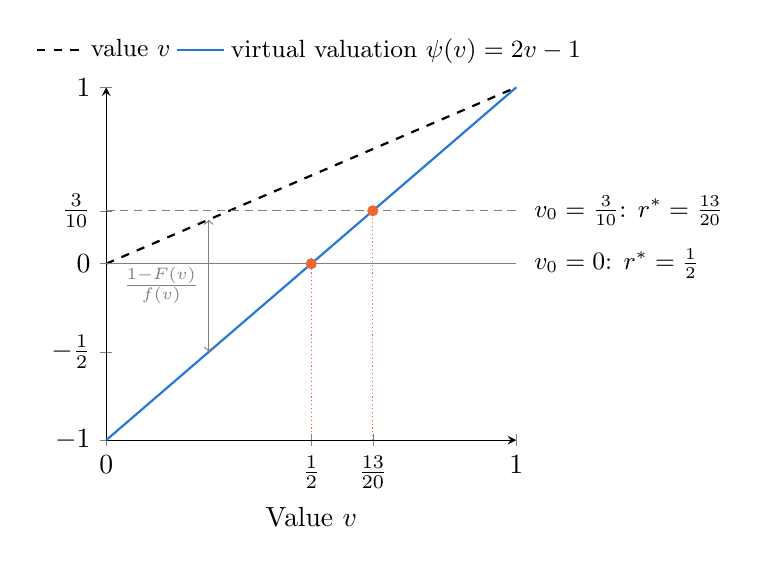
\begin{tikzpicture}
\begin{axis}[width=0.56\textwidth,height=0.5\textwidth,xmin=0,xmax=1,ymin=-1,ymax=1,
  axis lines=left,xlabel={Value $v$},ylabel={},
  xtick={0,0.5,0.65,1},xticklabels={$0$,$\frac12$,$\frac{13}{20}$,$1$},
  ytick={-1,-0.5,0,0.3,1},yticklabels={$-1$,$-\frac12$,$0$,$\frac{3}{10}$,$1$},clip=false,
  legend style={at={(0.5,1.04)},anchor=south,draw=none,fill=white,font=\small},legend columns=2,legend cell align=left]
\addplot[thick,black,dashed,domain=0:1] {x};
\addlegendentry{value $v$}
\addplot[thick,c14blue,domain=0:1] {2*x-1};
\addlegendentry{virtual valuation $\psi(v)=2v-1$}
\addplot[thin,gray,domain=0:1] {0};
\addplot[thin,gray,densely dashed,domain=0:1] {0.3};
\addplot[only marks,mark=*,c14orange,mark size=1.8pt] coordinates {(0.5,0) (0.65,0.3)};
\draw[densely dotted,c14orange] (axis cs:0.65,-1) -- (axis cs:0.65,0.3);
\draw[densely dotted,c14orange] (axis cs:0.5,-1) -- (axis cs:0.5,0);
\node[font=\small,anchor=west] at (axis cs:1.02,0.3) {$v_0=\frac{3}{10}$: $r^*=\frac{13}{20}$};
\node[font=\small,anchor=west] at (axis cs:1.02,0) {$v_0=0$: $r^*=\frac12$};
\draw[<->,gray] (axis cs:0.25,-0.5) -- (axis cs:0.25,0.25) node[midway,left,font=\footnotesize] {$\frac{1-F(v)}{f(v)}$};
\end{axis}
\end{tikzpicture}
\caption{Virtual valuation for values uniform on $[0,1]$. The gap between the value and the virtual valuation is the information rent $\frac{1-F(v)}{f(v)}=1-v$. The optimal reserve price is the value at which the virtual valuation equals the seller's value $v_0$, so it exceeds $v_0$.}\label{fig:14-virtual}
\end{figure}

\subsection{The cost of a reserve price: a worked example}\label{sec:14-optimal-example}

Let values be uniform on $[0,1]$, $v_0=0$ and $n=2$. Without a reserve price, revenue is $\E[V_{(1:2)}]=\frac13$. With the optimal reserve $r^*=\frac12$, \cref{prop:14-myerson} gives expected revenue
\[
\E\big[\max\{0,\psi(V_{(2:2)})\}\big]=\int_{\frac{1}{2}}^{1}(2v-1)\,2v\,dv=2\int_{\frac{1}{2}}^{1}(2v^2-v)\,dv=2\Big[\frac{2v^3}{3}-\frac{v^2}{2}\Big]_{\frac{1}{2}}^{1}=2\Big(\frac16+\frac{1}{24}\Big)=\frac{5}{12}.
\]
A direct computation in the second-price auction confirms the number. Both values exceed $\frac12$ with probability $\frac14$, and the price is then the lower value, with conditional mean $\frac23$. Exactly one value exceeds $\frac12$ with probability $\frac12$, and the price is then $\frac12$. Expected revenue is $\frac14\cdot\frac23+\frac12\cdot\frac12=\frac{5}{12}$, the same as the first-price revenue in \cref{ex:14-uniform-reserve}.

The gain to the seller comes at a cost. With probability $\frac14$ both values fall below $\frac12$ and the object is not sold, although the seller values it at zero. The expected surplus lost in this event is $\int_0^{\frac{1}{2}}v\,2v\,dv=\frac{1}{12}$. Total surplus falls from $\frac23$ to $\frac{7}{12}$, and the bidders' combined surplus falls from $\frac13$ to $\frac16$. The reserve price thus transfers $\frac{1}{12}$ from bidders to the seller and destroys another $\frac{1}{12}$. This exclusion of buyers who value the object more than the seller is the auction analogue of the deadweight loss of monopoly pricing.

The gain from the reserve shrinks quickly with the number of bidders. For $n$ uniform bidders,
\[
\int_{\frac{1}{2}}^{1}(2v-1)\,nv^{n-1}\,dv=\Big[\frac{2n\,v^{n+1}}{n+1}-v^n\Big]_{\frac{1}{2}}^{1}=\frac{n-1}{n+1}+\frac{1}{(n+1)2^n}.
\]
The second term is the gain over the no-reserve revenue $\frac{n-1}{n+1}$. The reserve binds only when at most one value exceeds it, and that event becomes rare as $n$ grows. \Cref{tab:14-reserve-uniform} reports the numbers.

\begin{table}[htbp]
\centering
\begin{threeparttable}
\caption{The value of the optimal reserve price and of one more bidder, with values uniform on $[0,1]$ and $v_0=0$.}\label{tab:14-reserve-uniform}
\small
\begin{tabular}{cccccc}
\toprule
 & \multicolumn{2}{c}{Expected revenue, $n$ bidders} & & & Absolute auction,\\
\cmidrule(lr){2-3}
$n$ & No reserve & Reserve $r^*=\frac12$ & $\Pr(\text{no sale})$ & Surplus lost & $n+1$ bidders\\
\midrule
1 & $0$ & $\frac{1}{4}$ & $\frac{1}{2}$ & $\frac{1}{8}$ & $\frac{1}{3}$\\[3pt]
2 & $\frac{1}{3}$ & $\frac{5}{12}$ & $\frac{1}{4}$ & $\frac{1}{12}$ & $\frac{1}{2}$\\[3pt]
3 & $\frac{1}{2}$ & $\frac{17}{32}$ & $\frac{1}{8}$ & $\frac{3}{64}$ & $\frac{3}{5}$\\[3pt]
4 & $\frac{3}{5}$ & $\frac{49}{80}$ & $\frac{1}{16}$ & $\frac{1}{40}$ & $\frac{2}{3}$\\[3pt]
5 & $\frac{2}{3}$ & $\frac{43}{64}$ & $\frac{1}{32}$ & $\frac{5}{384}$ & $\frac{5}{7}$\\
\bottomrule
\end{tabular}
\begin{tablenotes}
\footnotesize
\item Notes: Without a reserve price, revenue is $\frac{n-1}{n+1}$. With $r^*=\frac12$, revenue is $\frac{n-1}{n+1}+\frac{1}{(n+1)2^n}$, the revenue of the optimal mechanism. The probability of no sale is $2^{-n}$. Surplus lost is the expected value of the highest bidder when the object is not sold, $\frac{n}{n+1}2^{-(n+1)}$. The last column is the revenue of an English auction without reserve price and with $n+1$ bidders, $\frac{n}{n+2}$. With $n=1$ the optimal mechanism is a posted price of $\frac12$. All entries are exact.
\end{tablenotes}
\end{threeparttable}
\end{table}

\subsection{Competition versus mechanism design}\label{sec:14-optimal-bk}

The last column of \cref{tab:14-reserve-uniform} anticipates a striking result. In every row, an auction without a reserve price and with one more bidder beats the optimal mechanism.

\begin{proposition}[\citealp{BulowKlemperer1996}]\label{prop:14-bk}
Let \cref{ass:14-ipv} hold with symmetric bidders, a common regular distribution $F$ on $[\underline v,\bar v]$, and $\underline v\ge v_0$. Then an English auction without a reserve price and with $n+1$ bidders yields at least as much expected revenue as the optimal mechanism with $n$ bidders.
\end{proposition}

\begin{proof}
Let $R_n^*$ denote the seller's expected payoff in the optimal mechanism with $n$ bidders. Construct a mechanism for $n+1$ bidders as follows. Run the optimal $n$-bidder mechanism among bidders $1,\dots,n$. If it sells the object, stop. If it does not, give the object to bidder $n+1$ at the price $\underline v$. This mechanism is incentive compatible, since bidder $n+1$'s report affects nothing. It is individually rational, and every lowest type earns zero. It always sells the object.

By \eqref{eq:14-revenue-psi}, the constructed mechanism yields
\[
\E\Big[\sum_{i=1}^n\psi(V_i)q_i(\bm V)\Big]+\E\big[\psi(V_{n+1})\big]\Pr(\text{no sale among }1,\dots,n),
\]
where we used the independence of $V_{n+1}$ from the other values. Integration by parts gives $\E[\psi(V)]=\E[V]-\int_{\underline v}^{\bar v}(1-F(v))dv=\E[V]-(\E[V]-\underline v)=\underline v$. The optimal $n$-bidder mechanism yields the same first term plus $v_0\Pr(\text{no sale})$. Because $\underline v\ge v_0$, the constructed mechanism earns at least $R_n^*$.

Now consider all incentive compatible mechanisms for $n+1$ bidders that always sell and leave the lowest types with zero. By \eqref{eq:14-revenue-psi}, revenue is $\E[\sum_i\psi(V_i)q_i(\bm V)]$ with $\sum_iq_i=1$. It is maximized pointwise by awarding the object to the highest virtual valuation, which under regularity is the highest value. The English auction without reserve price does exactly this, and its lowest types earn zero. Hence its revenue is at least that of the constructed mechanism, which is at least $R_n^*$.
\end{proof}

For uniform values, the optimal mechanism with two bidders earns $\frac{5}{12}$, while an English auction with three bidders earns $\frac{3-1}{3+1}=\frac12$. Even a single buyer facing an optimal posted price yields only $\frac14$, below the $\frac13$ of a two-bidder auction. \Citet{BulowKlemperer1996} frame the result as auctions versus negotiations. A seller who can recruit one more serious bidder should do so rather than negotiate optimally with the bidders it has. Competition is worth more than bargaining power and knowledge of the value distribution. The result needs symmetric bidders, regular distributions and costless participation. \Cref{sec:14-entry} studies what changes when entry is costly.

The ranking also holds in data where its assumptions do not hold exactly. \Citet{RobertsSweeting2016} estimate a model of U.S.\ Forest Service timber auctions with asymmetric bidders and selective entry, in which entrants bid in a second-price auction. In their estimates, an additional bidder is worth more to the seller than an optimal reserve price \citep[Section~2.2, p.~92]{HortacsuPerrigne2021}.

\subsection{Asymmetric bidders: favoring the weak}\label{sec:14-optimal-asym}

With asymmetric bidders, the optimal mechanism discriminates. Consider two bidders and $v_0=0$. The weak bidder's value is uniform on $[0,1]$ and the strong bidder's value is uniform on $[0,2]$. The virtual valuations are
\[
\psi_w(v)=v-\frac{1-v}{1}=2v-1,\qquad \psi_s(v)=v-\frac{1-\frac{v}{2}}{\frac12}=2v-2.
\]
At equal values the weak bidder has the higher virtual valuation. By \cref{prop:14-myerson}, the weak bidder wins when $2v_w-1>\max\{2v_s-2,0\}$, that is, when $v_w>\frac12$ and $v_w>v_s-\frac12$. The strong bidder wins when $v_s>1$ and $v_s>v_w+\frac12$. The mechanism sets bidder-specific reserve prices, $\frac12$ for the weak bidder and $1$ for the strong bidder, and gives the weak bidder a head start of $\frac12$ in the competition.

\begin{figure}[htbp]
\centering
\begin{tikzpicture}[scale=2.4]
\fill[gray!25] (0,0) rectangle (0.5,1);
\fill[c14blue!18] (0.5,0) -- (1,0) -- (1,1.5) -- (0.5,1) -- cycle;
\fill[c14orange!15] (0,1) -- (0.5,1) -- (1,1.5) -- (1,2) -- (0,2) -- cycle;
\fill[pattern=north east lines,pattern color=c14blue] (0.5,0.5) -- (1,1) -- (1,1.5) -- (0.5,1) -- cycle;
\draw[thick] (0,0) rectangle (1,2);
\draw[thick,dashed] (0,0) -- (1,1);
\draw[thick] (0.5,0) -- (0.5,1) -- (1,1.5);
\draw[thick] (0,1) -- (0.5,1);
\node[font=\footnotesize] at (0.25,0.75) {no sale};
\node[font=\small,align=center] at (0.78,0.25) {weak\\wins};
\node[font=\small] at (0.45,1.55) {strong wins};
\draw[->,thin] (1.12,1.2) node[right,font=\footnotesize,align=left] {weak wins with\\the lower value} -- (0.85,1.1);
\node[font=\footnotesize,anchor=west] at (1.02,0.95) {$v_s=v_w$};
\node[font=\footnotesize,anchor=west] at (1.02,1.55) {$v_s=v_w+\frac12$};
\draw (0,0) -- (0,-0.04) node[below,font=\footnotesize] {$0$};
\draw (0.5,0) -- (0.5,-0.04) node[below,font=\footnotesize] {$\frac12$};
\draw (1,0) -- (1,-0.04) node[below,font=\footnotesize] {$1$};
\draw (0,1) -- (-0.04,1) node[left,font=\footnotesize] {$1$};
\draw (0,2) -- (-0.04,2) node[left,font=\footnotesize] {$2$};
\draw (0,0) -- (-0.04,0) node[left,font=\footnotesize] {$0$};
\node[below,font=\small] at (0.5,-0.3) {weak value $v_w$};
\node[rotate=90,font=\small] at (-0.3,1) {strong value $v_s$};
\end{tikzpicture}
\caption{The optimal allocation with a weak bidder, $V_w\sim U[0,1]$, and a strong bidder, $V_s\sim U[0,2]$, when $v_0=0$. The hatched region is where the weak bidder wins although the strong bidder has the higher value.}\label{fig:14-asym-optimal}
\end{figure}

\Cref{fig:14-asym-optimal} shows the regions. Values are uniform on the rectangle $[0,1]\times[0,2]$, so each probability is half the corresponding area. The object is not sold with probability $\frac14$. The weak bidder wins with probability $\frac{5}{16}$ and the strong bidder with probability $\frac{7}{16}$. With probability $\frac18$ the weak bidder wins although the strong bidder values the object more. The seller's expected revenue is $\E[\max\{0,\psi_w(V_w),\psi_s(V_s)\}]=\frac{31}{48}\approx 0.646$. A second-price auction without reserve price earns $\E[\min\{V_w,V_s\}]=\frac{5}{12}\approx 0.417$. \Cref{sec:14-asym} computes the first-price revenue in the same example. Expected total surplus is $\frac{11}{12}$ under the optimal mechanism, against $\frac{13}{12}$ under the efficient allocation. Each fraction follows from integrating over the regions in \cref{fig:14-asym-optimal}.

The logic resembles third-degree price discrimination, in which a monopolist charges less to the group with more elastic demand. In the auction the weak bidder plays the role of the elastic group. Here the head start for the weak bidder forces the strong bidder to pay more when it wins. The first-price auction also tilts outcomes toward weak bidders, although for different reasons (\cref{sec:14-asym}). This is one reason why it may raise more revenue than the second-price auction with asymmetric bidders. Bid preferences for small or domestic firms in public procurement have the same structure \citep{McAfeeMcMillan1989}, as \cref{sec:14-procurement} discusses.

\subsection{Entry fees}\label{sec:14-optimal-fees}

With symmetric independent private values, an entry fee can replace the reserve price. Suppose the seller runs a second-price auction without reserve price, values are bounded below by $\underline v=0$, and each participant pays a fee $e$. A bidder with value $v^*$ at the participation threshold wins only when no rival participates, which has probability $F(v^*)^{n-1}$, and then pays nothing. Its gross expected payoff is $v^*F(v^*)^{n-1}$, so the threshold solves $v^*F(v^*)^{n-1}=e$. Setting $e^*=r^*F(r^*)^{n-1}$ makes the threshold equal to $r^*$. The allocation is then the optimal one, and the threshold type earns zero. By \cref{prop:14-ret}, the entry fee $e^*$ yields the optimal revenue. With uniform values and $n=2$, $e^*=\frac12\cdot\frac12=\frac14$. Each bidder enters with probability $\frac12$, so fees bring in $2\cdot\frac12\cdot\frac14=\frac14$, and the price paid when both enter adds $\frac14\cdot\frac23=\frac16$. The total is $\frac{5}{12}$, as with the optimal reserve price.

With affiliated values the equivalence breaks down. \Citet{MilgromWeber1982} compare reserve prices and entry fees that screen out the same types, and \cref{sec:14-mw-reserve} presents their result. With costly entry before bidders learn their values, reserve prices and fees also affect how many bidders participate (\cref{sec:14-entry}). The optimal reserve depends on $F$, which the seller does not observe directly. \Cref{ch:auction-empirics} shows how $F$ can be recovered from bids.

\casehead{The original papers} \citet{Myerson1981} poses the general design problem. A seller faces bidders with independent private information and may use any selling procedure. He proves the revelation principle for this setting, derives the payment identity and revenue equivalence, and shows that the optimal mechanism allocates by virtual valuations, with ironing when they are not monotone.
\Citet{RileySamuelson1981} reach the optimal reserve price \eqref{eq:14-optimal-reserve} within the class of standard auctions and show that it is independent of the number of bidders. \Citet[p.~87]{HortacsuPerrigne2021} attribute the formula to both papers. \Citet[p.~1093]{MilgromWeber1982} credit the optimal auction to the self-selection approach of \citet{HarrisRaviv1981}, \citet{Myerson1981} and \citet{RileySamuelson1981}. \Citet{BulowRoberts1989} interpret virtual valuations as marginal revenues and recast optimal auction design as monopoly pricing. \Citet{BulowKlemperer1996} prove \cref{prop:14-bk} and draw the lesson that attracting bidders matters more than fine-tuning the mechanism.

\section{Affiliated Values I: Equilibrium Bidding}\label{sec:14-mw-eq}

The private-values theory of \cref{sec:14-spa,sec:14-fpa,sec:14-ret,sec:14-optimal} rests on two
assumptions. Each bidder knows the value of the object to itself, and values are statistically independent.
Many of the auctions that motivate the theory violate both. An oil company bidding for a drilling lease does
not know how much oil lies under the tract, and its geologists' estimate is correlated with the estimates of
its rivals. This section and the next study the model of \citet{MilgromWeber1982}, which drops both
assumptions at once and still delivers sharp predictions. Their model became the standard framework for
auctions with interdependent values, and we treat the paper as a deep dive.

This section sets out the questions, the model and the properties of affiliation, and then derives the
symmetric equilibria of the second-price, English and first-price auctions. It also covers bidders with
inferior information, including the one-informed-bidder model that \citet{HendricksPorter1988} take to
offshore oil data. \Cref{sec:14-mw-rank} uses these equilibria to rank the formats by expected revenue,
studies the seller's disclosure of information, reserve prices, entry fees and risk aversion, and assesses
the paper. We keep the book's conventions from \cref{sec:14-info}. Bidder $i$'s signal is $S_i$ (Milgrom and
Weber write $X_i$), other value-relevant variables are $\bm A=(A_1,\dots,A_m)$ (their $S$), and the seller's
information is $S_0$ (their $X_0$).

\subsection{The question and the setting}\label{sec:14-mw-question}

\citet[pp.~1089--1090]{MilgromWeber1982} open with two sets of questions. The first concerns design. Why do
the English, Dutch, first-price and second-price auctions coexist, and which one should a seller use in a
given circumstance? The second concerns the link with competitive theory. Do auction prices resemble
competitive prices, and do they approach them when there are many bidders? When bidders hold different
information about the intrinsic qualities of the object, do prices aggregate that information, as they do in
rational expectations models of markets? Answering either set requires a model in which one bidder's
information matters for the value that others place on the object.

The benchmark at the time was the independent private values model, which
\citet[pp.~1090--1093]{MilgromWeber1982} summarize in seven conclusions. All of them appear earlier in this
chapter.
\begin{enumerate}[label=(\arabic*)]
  \item The Dutch and first-price auctions are strategically equivalent (\cref{prop:14-dutch-fpa}).
  \item With private values, the second-price and English auctions are equivalent in a weaker sense. Each has
  a dominant strategy, bidding (or staying in up to) one's value, and the two lead to the same outcome
  (\cref{sec:14-spa}).
  \item The English and second-price auctions allocate the object to the bidder who values it most, so their
  outcomes are Pareto optimal. In symmetric models the Dutch and first-price auctions do so as well
  (\cref{sec:14-fpa}).
  \item All four formats yield the same expected revenue (\cref{prop:14-ret}).
  \item The self-selection approach explains this. Any mechanism that gives the object to the highest
  valuation and leaves the lowest type a zero payment yields the expected second-highest valuation
  (\cref{sec:14-ret}).
  \item For many common distributions, including the normal, exponential and uniform, the standard formats
  with a suitable reserve price or entry fee are optimal mechanisms (\cref{sec:14-optimal}).
  \item When bidders are risk averse, the seller strictly prefers the Dutch or first-price auction to the
  English or second-price auction (\cref{prop:14-risk-fpa}).
\end{enumerate}
For the design question this benchmark gives little guidance. Its main prediction is that the four common
formats raise the same expected price \citep[p.~1095]{MilgromWeber1982}.

Mineral rights are the leading example of a different environment \citep[Section~2.2]{MilgromWeber1982}.
To a first approximation the rights are worth the same to every bidder, and bidders differ only in their
estimates of this common value. \Cref{sec:14-winners-curse} described the resulting winner's curse and the
two results of the mineral rights literature that foreshadow the general theory. Prices can aggregate
dispersed information (\cref{rem:14-aggregation}), and a bidder's profit depends more on the privacy of its
information than on its accuracy (\cref{rem:14-privacy}). We prove a version of the second result in
\cref{sec:14-mw-inferior}.

The sale of a painting (\cref{sec:14-info-model}) shows why a general model is needed. Resale, prestige and
doubts about authenticity break private values, and related information breaks independence. The common
value model allows for statistical dependence but leaves no room for differences in tastes. Milgrom and Weber
build a model that contains both the private values and common value models and the intermediate cases
between them. Despite its generality, the model yields testable predictions
\citep[pp.~1095--1097]{MilgromWeber1982}.
\begin{enumerate}[label=(\roman*)]
  \item The Dutch and first-price auctions remain strategically equivalent.
  \item When bidders are uncertain about their own values, the English auction generates higher expected
  prices than the second-price auction. Bidders learn from the prices at which rivals drop out, which
  weakens the winner's curse and makes them bid more aggressively.
  \item When value estimates are positively dependent, the second-price auction generates higher expected
  prices than the first-price auction. The formats are ranked English, then second price, then Dutch and
  first price. Milgrom and Weber suggest that this ranking may explain an observation by Cassady. In his
  words, ``an estimated 75 per cent, or even more, of all auctions in the world are conducted on an
  ascending-bid basis'' \citep[p.~66, quoted in Milgrom and Weber 1982, p.~1095]{Cassady1967}.
  \item A seller with private information can commit to concealing it, reporting it fully, censoring it,
  summarizing it or adding noise to it. In the first-price, second-price and English auctions, reporting it
  fully maximizes the expected price.
  \item Holding fixed the set of bidders who participate, it pays to raise entry fees and lower reserve
  prices.
  \item With risk-averse bidders, the first-price and second-price auctions cannot be ranked in general. With
  constant absolute risk aversion, the English auction still beats the second-price auction and full
  disclosure remains optimal in both.
\end{enumerate}
The rest of this section and the next derive each prediction.

\subsection{The model}\label{sec:14-mw-model}

We work with the general symmetric model of \cref{sec:14-info-model} and maintain \cref{ass:14-mw}
throughout this section and the next. There are $n\ge 2$ bidders and one indivisible object. Bidder $i$
observes a real-valued signal $S_i$ with realization $s_i$, which we also call its \emph{value estimate}. The
vector $\bm A=(A_1,\dots,A_m)$ collects the other variables that affect the value of the object, such as an
expert appraisal or the tastes of future buyers. The value to bidder $i$ is $V_i=u(\bm A,S_i,\bm S_{-i})$,
which may depend on variables that bidder $i$ does not observe. Private values are the case $m=0$ and
$V_i=S_i$, and the pure common value model is the case $m=1$ and $V_i=A_1$. Bidders are risk neutral until
\cref{sec:14-mw-risk}. A bidder who wins and pays $b$ receives $V_i-b$, and losers receive zero.

By symmetry we can study bidder 1. Let $Y_1\ge Y_2\ge\dots\ge Y_{n-1}$ denote the order statistics of the
rivals' signals $S_2,\dots,S_n$, largest first. Because $u$ is symmetric in the rivals' signals, bidder 1's
value depends on them only through their order statistics:
\begin{equation}\label{eq:14-mw-V1}
  V_1=u(\bm A,S_1,Y_1,\dots,Y_{n-1}).
\end{equation}
The joint density of $(\bm A,S_1,Y_1,\dots,Y_{n-1})$ is \eqref{eq:14-joint-orderstat}, which is
$(n-1)!$ times the density $f$ restricted to ordered vectors of rival signals.

The function that drives all equilibria is the expected value of the object to bidder 1 when its signal is
$s$ and the highest rival signal is $y$:
\begin{equation}\label{eq:14-mw-v}
  v(s,y)=\E\left[V_1\mid S_1=s,\,Y_1=y\right].
\end{equation}
We write $F_{Y_1}(\cdot\mid s)$ and $f_{Y_1}(\cdot\mid s)$ for the conditional distribution function and
density of $Y_1$ given $S_1=s$, and $[\underline s,\bar s]$ for the support of each signal. Milgrom and Weber
add a \emph{nondegeneracy} assumption, namely that $\E[V_1\mid S_1=s,Y_1=y_1,\dots,Y_{n-1}=y_{n-1}]$ is
strictly increasing in $s$. It shortens proofs, and all results hold without it
\citep[p.~1100]{MilgromWeber1982}. A strategy for bidder $i$ is a function $\beta_i:[\underline s,\bar s]\to\R_+$
from signals to bids. We study symmetric equilibria in which every bidder uses the same strictly increasing
$\beta$.

\subsection{Properties of affiliation}\label{sec:14-mw-affil}

Affiliation was defined in \cref{def:14-affiliation}, and \cref{prop:14-affil-char} gave its
characterization for smooth densities (Milgrom and Weber's Theorem 1). \Cref{prop:14-affil-props} listed the
four further properties that the equilibrium analysis uses (their Theorems 2 to 5), and
\cref{sec:14-affiliation} proved part (iv), which concerns order statistics. We now prove the other three
parts, or sketch the proofs, in the generality that we need.

\begin{proof}[Proof of \cref{prop:14-affil-props}, parts (i) to (iii)]
\emph{Part (i).} We prove the case of strictly increasing, differentiable $g_j$, which covers our applications.
Let $\bm W=(g_1(Z_1),\dots,g_k(Z_k))$ and $\bm g^{-1}(\bm w)=(g_1^{-1}(w_1),\dots,g_k^{-1}(w_k))$. The
change-of-variables formula gives the density of $\bm W$:
\begin{equation*}
  f_{\bm W}(\bm w)=f\left(\bm g^{-1}(\bm w)\right)J(\bm w),\qquad
  J(\bm w)=\prod_{j=1}^k\frac{d g_j^{-1}(w_j)}{dw_j}.
\end{equation*}
Each $g_j^{-1}$ is increasing and acts on one coordinate, so
$\bm g^{-1}(\bm w\vee\bm w')=\bm g^{-1}(\bm w)\vee\bm g^{-1}(\bm w')$, and similarly for $\wedge$. The
affiliation of $f$ then gives
$f(\bm g^{-1}(\bm w\vee\bm w'))f(\bm g^{-1}(\bm w\wedge\bm w'))\ge f(\bm g^{-1}(\bm w))f(\bm g^{-1}(\bm w'))$.
For the Jacobian, the pair $\{\max\{w_j,w_j'\},\min\{w_j,w_j'\}\}$ equals the pair $\{w_j,w_j'\}$ in every
coordinate, so $J(\bm w\vee\bm w')J(\bm w\wedge\bm w')=J(\bm w)J(\bm w')$. Multiplying the two relations
proves the claim. If all $g_j$ are decreasing, then $\bm g^{-1}(\bm w\vee\bm w')=\bm g^{-1}(\bm w)\wedge
\bm g^{-1}(\bm w')$, and the argument goes through because \eqref{eq:14-affil-ineq} is symmetric in the roles
of $\vee$ and $\wedge$. Weakly monotone transformations can create atoms, and they require the general
definition of affiliation in Milgrom and Weber's Appendix.

\emph{Parts (ii) and (iii).} Milgrom and Weber derive both from the characterization of affiliation as
conditional association in \cref{prop:14-association}(b). For densities, \citet{KarlinRinott1980} prove
directly that integrating out a variable preserves \eqref{eq:14-affil-ineq}, which is part (ii). Part (iii)
follows from the conditional association inequality applied to $g=H$ and to indicators of increasing sets
\citep[see also][]{Whitt1982}. We prove (iii) in the bivariate case that we use most often. Let $(Z_1,Z_2)$
have an affiliated density, let $H$ be nondecreasing, and consider $\E[H(Z_2)\mid Z_1=z,\,Z_2\le x]$.
Conditional on $Z_1=z$ and $Z_2\le x$, $Z_2$ has density $\frac{f(y\mid z)}{F(x\mid z)}$ on $y\le x$. For
$z'>z$ the ratio of the densities under $z'$ and $z$ is $\frac{f(y\mid z')F(x\mid z)}{f(y\mid z)F(x\mid z')}$,
which is nondecreasing in $y$ by the monotone likelihood ratio property (\cref{prop:14-affil-mlrp}). A
likelihood ratio ordering implies first-order stochastic dominance, so the conditional mean of the
nondecreasing function $H$ rises with $z$. For $x'>x$, the ratio of the densities truncated at $x'$ and at
$x$ equals the constant $\frac{F(x\mid z)}{F(x'\mid z)}$ on $y\le x$ and is infinite on $(x,x']$. It is
nondecreasing in $y$, so the mean rises with $x$ as well.
\end{proof}

Two consequences are used repeatedly.

\begin{corollary}\label{cor:14-mw-v}
Under \cref{ass:14-mw}, $(S_1,Y_1)$ are affiliated, and $v(s,y)$ is nondecreasing in both arguments. Under
nondegeneracy, $v$ is strictly increasing in $s$.
\end{corollary}

\begin{proof}
Affiliation of $(S_1,Y_1)$ follows from parts (iv) and (ii) of \cref{prop:14-affil-props}. Let
\begin{equation*}
  \bar v(s,y_1,\dots,y_{n-1})=\E\left[V_1\mid S_1=s,\,Y_1=y_1,\dots,Y_{n-1}=y_{n-1}\right].
\end{equation*}
By \eqref{eq:14-mw-V1}, $\bar v$ is the conditional mean of the nondecreasing function $u$ of the affiliated
vector of \cref{prop:14-affil-props}(iv), so it is nondecreasing by part (iii). The law of iterated
expectations gives
\begin{equation*}
  v(s,y)=\E\left[\bar v(S_1,Y_1,\dots,Y_{n-1})\mid S_1=s,\,Y_1=y\right],
\end{equation*}
which is nondecreasing by part (iii) again. If $\bar v$ is strictly increasing in $s$ and $s'>s$, then
\begin{align*}
  v(s',y)&=\E[\bar v(s',y,Y_2,\dots,Y_{n-1})\mid S_1=s',Y_1=y]\\
  &>\E[\bar v(s,y,Y_2,\dots,Y_{n-1})\mid S_1=s',Y_1=y]\\
  &\ge\E[\bar v(s,y,Y_2,\dots,Y_{n-1})\mid S_1=s,Y_1=y]=v(s,y).\qedhere
\end{align*}
\end{proof}

\begin{lemma}[{\citealp[Lemma~1]{MilgromWeber1982}}]\label{lem:14-mw-lemma1}
Under \cref{ass:14-mw}, $\frac{F_{Y_1}(y\mid z)}{f_{Y_1}(y\mid z)}$ is nonincreasing in $z$.
\end{lemma}

\begin{proof}
Let $g(z,y)$ be the joint density of $(S_1,Y_1)$, which is affiliated by \cref{cor:14-mw-v}. Take
$\alpha\le y$ and $z'\le z$, and apply \eqref{eq:14-affil-ineq} to the points $(z,\alpha)$ and $(z',y)$.
Their componentwise maximum is $(z,y)$ and their minimum is $(z',\alpha)$, so
\begin{equation*}
  g(z,y)\,g(z',\alpha)\ge g(z,\alpha)\,g(z',y).
\end{equation*}
Dividing both sides by the marginal densities of $S_1$ at $z$ and $z'$ turns joint densities into
conditional densities:
\begin{equation*}
  f_{Y_1}(y\mid z)\,f_{Y_1}(\alpha\mid z')\ge f_{Y_1}(\alpha\mid z)\,f_{Y_1}(y\mid z').
\end{equation*}
Rearranging gives
$\frac{f_{Y_1}(\alpha\mid z)}{f_{Y_1}(y\mid z)}\le\frac{f_{Y_1}(\alpha\mid z')}{f_{Y_1}(y\mid z')}$ for
every $\alpha\le y$. Integrating over $\alpha\in[\underline s,y]$ yields
$\frac{F_{Y_1}(y\mid z)}{f_{Y_1}(y\mid z)}\le\frac{F_{Y_1}(y\mid z')}{f_{Y_1}(y\mid z')}$.
\end{proof}

\subsection{The second-price auction}\label{sec:14-mw-spa}

Suppose bidders $2,\dots,n$ use strategies $\beta_j$, and let $M_1=\max_{j\ne1}\beta_j(S_j)$ be the highest
rival bid. Bidder 1 wins the second-price auction if its bid exceeds $M_1$, and then it pays $M_1$. With
signal $s$ it chooses $b$ to solve
\begin{equation*}
  \max_b\ \E\left[(V_1-M_1)\,\indic\{M_1<b\}\mid S_1=s\right].
\end{equation*}

\begin{proposition}[{\citealp[Theorem~6]{MilgromWeber1982}}]\label{prop:14-mw-spa}
Under \cref{ass:14-mw}, the strategy $\beta^{SP}(s)=v(s,s)$ used by every bidder is a symmetric equilibrium
of the second-price auction.
\end{proposition}

\begin{proof}
Let bidders $2,\dots,n$ use $\beta^{SP}$. Since $\beta^{SP}$ is increasing, the highest rival bid is
$M_1=\beta^{SP}(Y_1)=v(Y_1,Y_1)$. Bidder 1's expected payoff from a bid $b$ in the range of $\beta^{SP}$ is
\begin{align*}
  &\E\left[(V_1-\beta^{SP}(Y_1))\indic\{\beta^{SP}(Y_1)<b\}\mid S_1=s\right]\\
  &\qquad=\E\left[\E\left[(V_1-\beta^{SP}(Y_1))\indic\{\beta^{SP}(Y_1)<b\}\mid S_1,Y_1\right]\mid S_1=s\right]\\
  &\qquad=\E\left[\left(v(S_1,Y_1)-v(Y_1,Y_1)\right)\indic\{\beta^{SP}(Y_1)<b\}\mid S_1=s\right]\\
  &\qquad=\int_{\underline s}^{(\beta^{SP})^{-1}(b)}\left[v(s,\alpha)-v(\alpha,\alpha)\right]f_{Y_1}(\alpha\mid s)\,d\alpha.
\end{align*}
The first line applies the law of iterated expectations. The second uses the definition \eqref{eq:14-mw-v}
and the fact that $\beta^{SP}(Y_1)$ is known once $Y_1$ is. Because $v$ is increasing in its first argument
(\cref{cor:14-mw-v}), the integrand is positive for $\alpha<s$ and negative for $\alpha>s$. The integral is
therefore maximized by choosing the upper limit equal to $s$, that is, $b=\beta^{SP}(s)$. A bid above
$\beta^{SP}(\bar s)$ wins against every rival and gives the integral up to $\bar s$. A bid below
$\beta^{SP}(\underline s)$ never wins. Neither does better.
\end{proof}

The equilibrium bid is the expected value of the object conditional on the bidder's own signal and on the
event that the strongest rival has the same signal. A bidder's bid matters only when it ties the highest rival
bid, because otherwise a small change does not affect the outcome or the price. In a symmetric increasing
equilibrium, a tie means $Y_1=s$. \citet[eq.~(2.3)]{AtheyHaile2007} call $v(s,s)$ the expectation
conditional on the bid being \emph{pivotal}. The bid embeds the correction for the winner's curse. With
private values $v(s,s)=s$, and the equilibrium reduces to the dominant strategy of \cref{prop:14-spa-dominant}.
With common values the equilibrium is not in dominant strategies. The best bid depends on what winning
reveals, and that depends on rivals' strategies. When bidder 1 wins, it pays $v(Y_1,Y_1)$, where $Y_1$ is the
second-highest signal among all bidders. \Citet[footnote~17, p.~1100]{MilgromWeber1982} note that their analysis
of the second-price auction is very similar to that of \citet{Milgrom1981a}, in a somewhat different setup.
Their Theorems~6 and~7, our \cref{prop:14-mw-spa,prop:14-mw-garbling}, were first proved there.

\begin{example}[Mineral rights with uniform noise]\label{ex:14-mineral}
Return to the mineral rights model of \cref{ex:14-wc-uniform}. The value is common, $V_i=V$, and the
signals are $S_i=V+\epsilon_i$, where the noise terms $\epsilon_i$ are \iid\ uniform on $[-\omega,\omega]$
and independent of $V$. Let $V$ be uniform on an interval much wider
than $\omega$, and consider signals far from its ends. This is the \emph{diffuse prior} idealization: given
the signals, the prior is flat over every value that the signals allow. The noise density
$\frac{1}{2\omega}\indic\{|x-v|\le\omega\}$ satisfies \eqref{eq:14-affil-ineq}, because the band
$\{(x,v):|x-v|\le\omega\}$ contains the componentwise maximum and minimum of any two of its points. So the
example fits \cref{ass:14-mw}. Nondegeneracy fails, since the posterior mean of $V$ depends only on the
highest and lowest signals, but the results do not need it.

We compute $v(s,s)$. Given $V$, the event $\{S_1=s,Y_1=s\}$ has likelihood
$f(s\mid V)\cdot(n-1)F(s\mid V)^{n-2}f(s\mid V)$, where $f(s\mid V)=\frac{1}{2\omega}$ and
$F(s\mid V)=\frac{s-V+\omega}{2\omega}$ for $V\in[s-\omega,s+\omega]$. With a flat prior, the posterior
density of $V$ is proportional to $(s+\omega-V)^{n-2}$ on $[s-\omega,s+\omega]$. Substitute
$t=s+\omega-V\in[0,2\omega]$. The density of $t$ is $\frac{(n-1)t^{n-2}}{(2\omega)^{n-1}}$, with mean
\begin{equation*}
  \E[t]=\int_0^{2\omega}t\,\frac{(n-1)t^{n-2}}{(2\omega)^{n-1}}\,dt=\frac{n-1}{n}\,2\omega.
\end{equation*}
Hence
\begin{equation}\label{eq:14-mineral-spa}
  \beta^{SP}(s)=v(s,s)=s+\omega-\frac{2\omega(n-1)}{n}=s-\omega\,\frac{n-2}{n}.
\end{equation}
The estimate is unbiased, $\E[V\mid S_1=s]=s$, yet the bidder shades by $\omega\frac{n-2}{n}$. The shading
grows with $n$ and approaches $\omega$. With more rivals, tying the highest of them is worse news about $V$.
With private values the number of bidders does not affect the second-price bid at all. With $n=2$ the
bid equals $s$, because tying the only rival means two signals both equal to $s$.
\end{example}

The pivotal value is the object that empirical tests for common values target. Write $V(x,x,N)$ for
$\E[V_i\mid S_i=x,\ \max_{j\ne i}S_j=x]$ with $N$ bidders, which is $v(x,x)$ of \eqref{eq:14-mw-v}. In a
first-price auction, \citet{LaffontVuong1996} show that the inverse equilibrium strategy recovers it from bids.
In the notation of \citet[Section~2.3, p.~93]{HortacsuPerrigne2021},
\begin{equation*}
  V(x,x,N)=B+\frac{G_{B_{\max}\mid B}(B\mid B)}{g_{B_{\max}\mid B}(B\mid B)},
\end{equation*}
where $B$ is the bidder's bid and $B_{\max}$ the highest rival bid. This is \eqref{eq:14-apv-foc} below, read
with common values. With private values the left side is the bidder's own value. \Citet{HaileHongShum2003}
show that, with exogenous participation, $V(x,x,N)$ falls strictly in $N$ under common values and does not vary
with $N$ under private values. \Cref{ex:14-mineral} displays the first case. By \eqref{eq:14-mineral-spa}, the
pivotal value $s-\omega\frac{n-2}{n}$ falls in $n$ at every signal, while with private values it equals $s$
for every $n$. The test compares the estimated distributions of pivotal values across auctions with different
numbers of bidders (\cref{ch:auction-empirics}). The bids themselves are a poor guide. A decline of bids in the
number of bidders is a misleading test for the winner's curse \citep{Laffont1997}. \Citet{PinkseTan2005} show
that affiliated private values can make bids rise or fall with competition \citep[footnote~10,
p.~93]{HortacsuPerrigne2021}.

\begin{example}[Affiliated private values]\label{ex:14-apv}
Let $n=2$, $V_i=S_i$, and let the signals have the joint density $f(s_1,s_2)=\frac{4}{5}(1+s_1s_2)$ on
$[0,1]^2$, introduced in \cref{ex:14-affil}(d). The cross-partial of $\ln f$ is $\frac{1}{(1+s_1s_2)^2}>0$, so
the values are affiliated. The correlation between them is small, $\frac{2}{37}\approx0.054$. With private
values $v(s,y)=s$, so the second-price bid is $\beta^{SP}(s)=s$. For later use, the marginal density of $S_1$
is $\frac{2}{5}(2+s)$, and the conditional density and distribution function of $Y_1=S_2$ given $S_1=s$ are
\begin{equation}\label{eq:14-apv-cond}
  f_{Y_1}(y\mid s)=\frac{2(1+sy)}{2+s},\qquad F_{Y_1}(y\mid s)=\frac{y(2+sy)}{2+s}.
\end{equation}
\end{example}

\subsection{Bidders with inferior information}\label{sec:14-mw-inferior}

How much is information worth when someone else has it too? \citet[p.~1101]{MilgromWeber1982} answer this
in the \emph{generalized mineral rights model}, in which $V_1=\dots=V_n=V$. It differs from the mineral rights
model because the estimates need not be independent conditional on $V$. Suppose an $(n+1)$st bidder enters
with an estimate $S_{n+1}$ of $V$. We say that $S_{n+1}$ is a \emph{garbling} of $(S_1,Y_1)$ if the joint
density of $(V,S_1,\dots,S_n,S_{n+1})$ factors as $g(V,S_1,\dots,S_n)\,h(S_{n+1}\mid S_1,Y_1)$. This holds,
for example, if bidder $n+1$ bases its estimate only on information that bidder 1 also has.

\begin{proposition}[{\citealp[Theorem~7]{MilgromWeber1982}}]\label{prop:14-mw-garbling}
In the generalized mineral rights model, let $S_{n+1}$ be a garbling of $(S_1,Y_1)$, and let bidders
$1,\dots,n$ use the $n$-bidder equilibrium strategy $\beta^{SP}$ of \cref{prop:14-mw-spa}. Then bidder $n+1$
has no strategy that earns a positive expected payoff. Consequently, the profile in which bidders
$1,\dots,n$ use $\beta^{SP}$ and bidder $n+1$ bids zero is an equilibrium of the $(n+1)$-bidder
second-price auction.
\end{proposition}

\begin{proof}
Let $Z=\max\{S_1,Y_1\}$ be the highest signal among bidders $1,\dots,n$. If bidder $n+1$ bids $b$, it wins
when $\beta^{SP}(Z)<b$ and then pays $\beta^{SP}(Z)=v(Z,Z)$. Its expected payoff conditional on its
estimate and on winning is
\begin{align*}
  \E\left[V-\beta^{SP}(Z)\mid S_{n+1},\,\beta^{SP}(Z)<b\right]
  &=\E\left[\E\left[V-\beta^{SP}(Z)\mid S_1,Y_1,S_{n+1}\right]\mid S_{n+1},\,\beta^{SP}(Z)<b\right]\\
  &=\E\left[v(S_1,Y_1)-v(Z,Z)\mid S_{n+1},\,\beta^{SP}(Z)<b\right].
\end{align*}
The second line uses $\E[V\mid S_1,Y_1,S_{n+1}]=\E[V\mid S_1,Y_1]=v(S_1,Y_1)$, which is what the garbling
condition delivers. Since $Z\ge S_1$, $Z\ge Y_1$ and $v$ is nondecreasing in both arguments,
$v(S_1,Y_1)\le v(Z,Z)$. The conditional expected payoff is therefore nonpositive for every bid. Bidding zero
earns zero, so it is a best response. Against a bid of zero, the payoffs of bidders $1,\dots,n$ are the same
as in the $n$-bidder auction, so $\beta^{SP}$ remains a best response for them.
\end{proof}

Information that a rival also holds earns no rent. Bidder $n+1$'s estimate adds nothing to what bidder 1
knows, and whenever it wins it pays at least the expected value of the object given everything the
others know. We now turn to a model in which one bidder has private information and the rest share only
public information. It was introduced by \citet{Wilson1967} and characterized by
\citet{EngelbrechtWiggansMilgromWeber1983}. \citet{HendricksPorter1988} restate it and test it on federal
auctions of offshore drainage leases, tracts adjacent to tracts where oil has been found. Oil and gas leases
are the classic common value auction, and they are usually sold by first-price sealed bid
\citep[Section~4, p.~124]{HortacsuPerrigne2021}. We present their
version with symmetric valuations and leave the evidence to \cref{ch:auction-empirics}.

\casehead{The model} A tract has common value $V$. One \emph{informed} bidder, the owner of the
neighboring tract in the application, observes a private signal $X$ and a public signal $Z$. A set of $n\ge
1$ \emph{uninformed} bidders observe only $Z$. We fix $z$ and suppress it. The informed bidder's information
is summarized by $H=\E[V\mid X,Z]$, which has an atomless distribution $F_H$ with density $f_H$, support
$[\underline h,\bar h]$ (possibly unbounded above), and finite mean $\mu_H$. The value is common and the
uninformed observe only $Z$. By the law of iterated expectations, an uninformed bidder's expected value of
the tract conditional on any event about $X$ equals the conditional mean of $H$ on that event. The seller
sets a reserve price $r$ with $\underline h\le r<\mu_H$, and a bid of zero means no bid. The informed bidder
uses a bid function $\sigma(h)$, strictly increasing and differentiable where it exceeds $r$, with inverse
$\phi$ on that range. Uninformed bidder $i$ randomizes according to a distribution function $G_i$ on the
nonnegative reals. The highest uninformed bid then has distribution function $G(b)=\prod_{i=1}^nG_i(b)$.

When $G$ has no atom at $b\ge r$, the informed bidder with estimate $h$ who bids $b$ earns
\begin{equation}\label{eq:14-hp-informed}
  (h-b)\,G(b),
\end{equation}
which is equation (1) of \citet{HendricksPorter1988} at $b=\sigma(h)$. Uninformed bidder $i$ who bids $b>r$
wins when the informed bid is lower, that is, when $H<\phi(b)$. Its expected payoff is
\begin{equation}\label{eq:14-hp-uninformed}
  \E\left[(H-b)\indic\{H<\phi(b)\}\right]\prod_{j\ne i}G_j(b)
  =F_H(\phi(b))\left(\E[H\mid H<\phi(b)]-b\right)\prod_{j\ne i}G_j(b),
\end{equation}
which is their equation (2). \citet{HendricksPorter1988} also allow the uninformed bidders' value to be
lower by a constant $c\ge0$, reflecting cost differences or the neighbor's ability to internalize drainage
externalities. We set $c=0$ throughout.

\casehead{Finding the equilibrium} Three conditions pin down the equilibrium. First, uninformed bidders mix,
so they must be indifferent among all bids in the support of their mixture. In equilibrium their expected
profit is zero \citep[p.~869]{HendricksPorter1988}. At a bid $b>r$ in that support,
\eqref{eq:14-hp-uninformed} is zero only if $b=\E[H\mid H<\phi(b)]$. Writing $h'=\phi(b)$, this says that the
informed bidder's bid function is
\begin{equation*}
  \sigma(h')=\E[H\mid H\le h'].
\end{equation*}
Second, this function lies below $r$ for low estimates. Define $\hat h$ by $\E[H\mid H<\hat h]=r$, which
exists because $\E[H\mid H<h]$ rises continuously from $\underline h$ to $\mu_H$. Informed types between $r$ and
$\hat h$ cannot use the formula, and they bid the reserve price instead. Types below $r$ would lose money at
any admissible bid and abstain. Third, the informed bidder's first-order condition for \eqref{eq:14-hp-informed}
is $G(b)=(h-b)G'(b)$ at $b=\sigma(h)$. Try $G(\sigma(h))=F_H(h)$. Differentiating gives
$G'(\sigma(h))\sigma'(h)=f_H(h)$, so the first-order condition becomes
\begin{equation*}
  \sigma'(h)=\left(h-\sigma(h)\right)\frac{f_H(h)}{F_H(h)}.
\end{equation*}
The bid function from the first condition satisfies exactly this equation:
\begin{equation*}
  \sigma(h)=\frac{1}{F_H(h)}\int_{\underline h}^h x f_H(x)\,dx
  \quad\Longrightarrow\quad
  \sigma'(h)=\frac{h f_H(h)}{F_H(h)}-\frac{f_H(h)}{F_H(h)}\,\sigma(h)
  =\left(h-\sigma(h)\right)\frac{f_H(h)}{F_H(h)}.
\end{equation*}
So the highest uninformed bid must be distributed exactly like the informed bid on the range above $r$.

\begin{proposition}[{\citealp{EngelbrechtWiggansMilgromWeber1983} and \citealp[Theorem, p.~869]{HendricksPorter1988}}]\label{prop:14-emw}
Let $c=0$. A profile is an equilibrium of the first-price auction if and only if two conditions hold. The
informed bidder uses
\begin{equation*}
  \sigma^*(h)=\begin{cases}
  \E[H\mid H\le h] & h>\hat h,\\
  r & r\le h\le\hat h,\\
  \text{no bid} & h<r.
  \end{cases}
\end{equation*}
The highest uninformed bid has the distribution function
\begin{equation*}
  G^*(b)=\begin{cases}
  F_H(\hat h) & 0\le b\le r,\\
  F_H(\phi^*(b)) & r<b<\mu_H,\\
  1 & b\ge\mu_H.
  \end{cases}
\end{equation*}
Here $\hat h$ solves $\E[H\mid H<\hat h]=r$ and $\phi^*$ is the inverse of $\sigma^*$ on $(\hat h,\bar h)$.
The uninformed bidders earn zero expected profit. Their individual strategies are indeterminate, and only
the distribution of their highest bid is pinned down.
\end{proposition}

\begin{proof}
We prove that the profile is an equilibrium. The converse is in \citet{EngelbrechtWiggansMilgromWeber1983}
and the Appendix of \citet{HendricksPorter1988}.

\emph{Uninformed bidders.} Take uninformed bidder $i$ and any profile of the others with highest bid distributed as
$G^*$. For $b\in(r,\mu_H)$, $\phi^*(b)$ is well defined and $b=\E[H\mid H\le\phi^*(b)]$, so the first factor in
\eqref{eq:14-hp-uninformed} is zero. Every such bid earns zero. A bid of exactly $r$ wins when $H<r$ and ties
with informed types in $[r,\hat h]$. With random tie-breaking it earns at most
\begin{equation*}
  \E\left[(H-r)\indic\{H<r\}\right]+\frac{1}{2}\E\left[(H-r)\indic\{r\le H\le\hat h\}\right]
  =-\frac{1}{2}\E\left[(H-r)\indic\{r\le H\le\hat h\}\right]\le0,
\end{equation*}
times the probability that no other uninformed bidder bids more. The equality uses
$\E[(H-r)\indic\{H<\hat h\}]=0$, which is the definition of $\hat h$. A bid $b\ge\mu_H$ wins for sure and
earns $\mu_H-b\le0$. Abstaining also earns zero. So every mixture over no bid and bids in $(r,\mu_H)$ is a best response.

\emph{Informed bidder.} Against $G^*$, mimicking a type $x>\hat h$ gives the informed type $h$ the payoff
$\Pi(x;h)=(h-\sigma^*(x))F_H(x)$. Using $\sigma^{*\prime}(x)F_H(x)=(x-\sigma^*(x))f_H(x)$,
\begin{equation*}
  \frac{\partial\Pi(x;h)}{\partial x}=-\sigma^{*\prime}(x)F_H(x)+\left(h-\sigma^*(x)\right)f_H(x)
  =f_H(x)\,(h-x).
\end{equation*}
So for $h>\hat h$ the best $x$ is $x=h$. For $h\le\hat h$ the best $x\ge\hat h$ is $x=\hat h$, which yields
$(h-r)F_H(\hat h)$. This equals the payoff from bidding $r$, which wins exactly when no uninformed bidder bids,
an event of probability $G^*(r)=F_H(\hat h)$. Bids in $(r,\sigma^*(\hat h^+))$ do not exist, because
$\sigma^*(\hat h^+)=r$. Bids above $\mu_H$ win for sure and are worse than bids just below $\mu_H$. For
$h\ge r$, bidding $r$ beats abstaining because $(h-r)F_H(\hat h)\ge0$. For $h<r$, every admissible bid
$b\ge r>h$ loses money when it wins, so abstaining is optimal.
\end{proof}

Integrating by parts, $\int_{\underline h}^h x\,dF_H(x)=hF_H(h)-\int_{\underline h}^hF_H(x)\,dx$, so for
$h>\hat h$
\begin{equation}\label{eq:14-hp-shading}
  \sigma^*(h)=h-\frac{\int_{\underline h}^hF_H(x)\,dx}{F_H(h)}.
\end{equation}
This is equation (4) of \citet{HendricksPorter1988} with $c=0$ (they write the lower limit as $-\infty$). The
integral term is the amount by which the informed bidder shades its bid below its estimate. When the reserve
price does not bind ($r=\underline h$, so $\hat h=\underline h$), \eqref{eq:14-hp-shading} is the
Riley-Samuelson bid \eqref{eq:14-rs-bid} for two bidders with values drawn independently from $F_H$. The
informed bidder behaves as if it faced one private-value rival whose value is an independent copy of its
own. The uninformed bidders, taken together, replicate the bid distribution of that fictitious rival. The
public signal matters for the shading term even when it adds nothing to the informed bidder's estimate,
because it shapes the rivals' behavior \citep[p.~870]{HendricksPorter1988}.

Why must the uninformed bidders randomize? If they used a predictable bid, the informed bidder would top it
whenever the tract was worth more and stay out otherwise. The uninformed would then win only tracts worth less
than their bids and lose money on average \citep[p.~869]{HendricksPorter1988}. Randomization makes the
informed bidder lose some profitable tracts. The mixed equilibrium can be read as the limit of pure-strategy
equilibria of a game in which the uninformed bidders have slightly informative private signals
\citep[pp.~869--870]{HendricksPorter1988}.

The model makes sharp predictions. The informed bidder wins when $h>\hat h$ and the highest uninformed bid is
below $\sigma^*(h)$, which has probability $G^*(\sigma^*(h))=F_H(h)$. It also wins when $r\le h\le\hat h$ and
no uninformed bidder bids, which has probability $F_H(\hat h)$. Its unconditional probability of winning is
\begin{align*}
  \Pr(\text{informed wins})
  &=\int_{\hat h}^{\bar h}F_H(h)f_H(h)\,dh+\left[F_H(\hat h)-F_H(r)\right]F_H(\hat h)\\
  &=\frac{1}{2}\left[1-F_H(\hat h)^2\right]+F_H(\hat h)^2-F_H(\hat h)F_H(r)\\
  &=\frac{1}{2}+\frac{1}{2}F_H(\hat h)^2-F_H(\hat h)F_H(r).
\end{align*}
Nobody bids with probability $F_H(r)F_H(\hat h)$. Conditional on at least one bid, the informed bidder wins
with probability
\begin{equation}\label{eq:14-hp-winprob}
  \frac{\frac{1}{2}+\frac{1}{2}F_H(\hat h)^2-F_H(\hat h)F_H(r)}{1-F_H(\hat h)F_H(r)}
  =\frac{1}{2}+\frac{\frac{1}{2}F_H(\hat h)\left[F_H(\hat h)-F_H(r)\right]}{1-F_H(\hat h)F_H(r)}
  \ \ge\ \frac{1}{2},
\end{equation}
which is the expression on p.~870 of \citet{HendricksPorter1988}. The second form follows from splitting
the numerator as
\begin{equation*}
  \frac{1}{2}+\frac{1}{2}F_H(\hat h)^2-F_H(\hat h)F_H(r)=\frac{1}{2}\bigl[1-F_H(\hat h)F_H(r)\bigr]
  +\frac{1}{2}F_H(\hat h)\bigl[F_H(\hat h)-F_H(r)\bigr]
\end{equation*}
and dividing each part by the denominator. \citet[pp.~870--871]{HendricksPorter1988} list seven predictions, in the following order.
\begin{enumerate}[label=(\alph*)]
  \item The informed bidder abstains less often than the uninformed bidders do, since $F_H(r)\le F_H(\hat h)$.
  \item The informed bidder wins at least half of the auctions with a bid, by \eqref{eq:14-hp-winprob}.
  \item The uninformed bidders earn zero expected profit overall. They lose money on tracts where the informed
  bidder does not bid and earn money on tracts where it does.
  \item The informed bidder earns an information rent.
  \item The ex ante bid distributions, before $X$ is realized, are approximately the same. In our version
  with $c=0$, the informed bid is at most $\sigma^*(h)$ with probability $F_H(h)$ for $h>\hat h$, and
  $G^*(\sigma^*(h))=F_H(h)$. Above $r$ the informed bid and the highest uninformed bid therefore have the same
  distribution. They differ only in how the mass $F_H(\hat h)$ at or below $r$ splits between abstaining and
  bidding $r$.
  \item The number of uninformed bidders does not affect the informed bidder's strategy or the distribution of
  the highest uninformed bid. This is convenient empirically, because only uninformed bidders who choose to
  bid are observed.
  \item The informed bidder's bid rises with the public signal when a larger public signal is good news. By
  \eqref{eq:14-hp-shading}, a bidder with estimate $h>\hat h$ bids $\sigma^*(h)=\E[H\mid H<h]$, computed under the
  distribution of $H$ given the public signal. When that distribution has the MLRP in the public signal, this
  conditional mean rises with the signal \citep[p.~870]{HendricksPorter1988}.
\end{enumerate}

\begin{figure}[htbp]
  \centering
  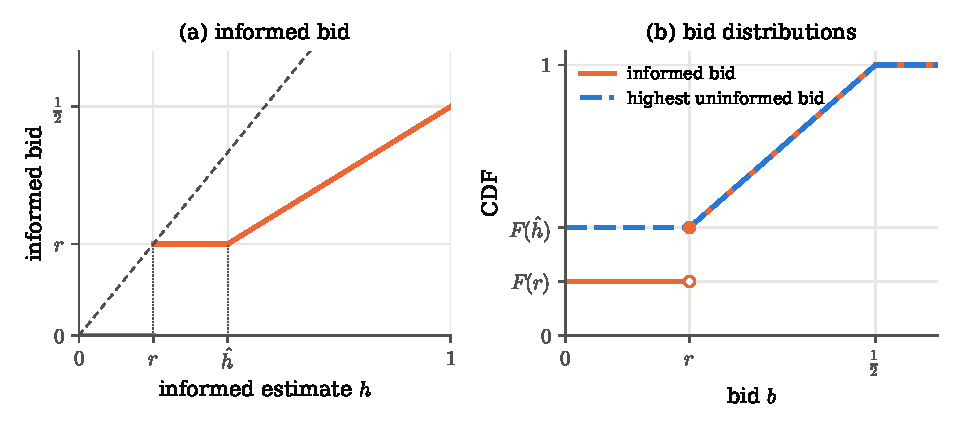
\includegraphics[width=0.95\textwidth]{figures/ch14/emw_equilibrium.pdf}
  \caption{Equilibrium with one informed bidder, for $H$ uniform on $[0,1]$ and reserve price $r=0.2$.
  Panel (a): the informed bid function, which is zero (no bid) below $r$, equal to $r$ on $[r,\hat h]$ with
  $\hat h=0.4$, and $\frac{h}{2}$ above $\hat h$. Panel (b): the distribution functions of the informed bid and
  of the highest uninformed bid. They coincide above $r$ and differ only in their masses at zero and at
  $r$.}\label{fig:14-emw}
\end{figure}

A numerical example makes the predictions concrete (\cref{fig:14-emw}). Let $H$ be uniform on $[0,1]$ and
$r=0.2$. Then $\E[H\mid H<\hat h]=\frac{\hat h}{2}=r$ gives $\hat h=0.4$, and $\sigma^*(h)=\frac{h}{2}$ for
$h>0.4$. The uninformed bidders abstain with probability $0.4$, and otherwise their highest bid has
distribution function $G^*(b)=2b$ on $(0.2,0.5]$. The informed bidder wins half of all auctions and $0.5435$
of the auctions with a bid, by \eqref{eq:14-hp-winprob}. Its expected profit is
$\int_{0.4}^1\frac{h}{2}\,h\,dh+0.4\int_{0.2}^{0.4}(h-0.2)\,dh=0.156+0.008=0.164$. The tract is sold unless
$H<r$ and no uninformed bidder bids, so expected surplus is $0.5-0.2\times0.4\times0.1=0.492$. The seller's
expected revenue is $0.492-0.164=0.328$. The uninformed bidders lose $0.15$ per tract on the tracts where the
informed bidder abstains and gain $0.0375$ per tract on the others, which nets to zero. These numbers come from
the script \texttt{emw\_example.py}, which also confirms them by simulation.

\Cref{prop:14-mw-garbling,prop:14-emw} make the same point from two sides. A bidder whose information is a
garbling of a rival's information earns nothing, and a bidder with exclusive information earns a rent even
against many rivals. The value of information in an auction lies in its privacy.

\subsection{The English auction}\label{sec:14-mw-english}

Milgrom and Weber model the English auction as the Japanese button auction of
\cref{def:14-button}. The price rises continuously from zero, the price and the number of active bidders are
displayed at all times, and exits are public and irrevocable. When one bidder remains, it wins and pays the
price at which the last rival left. With two bidders the English and second-price auctions are strategically
equivalent (\cref{prop:14-english-spa-n2}). With three or more bidders, the prices at which bidders drop out
convey information to those who remain, and the two formats differ.

Suppose $k$ bidders have quit, at prices $p_1\le\dots\le p_k$. A strategy for bidder $i$ specifies, for each
such history, the price $\beta_k(s_i\mid p_1,\dots,p_k)\ge p_k$ at which it will quit if nobody else quits
first. \citet[eqs.~(5)--(6)]{MilgromWeber1982} define the strategy $\beta^E=(\beta^E_0,\dots,
\beta^E_{n-2})$ iteratively. Before any exit,
\begin{equation}\label{eq:14-mw-english0}
  \beta^E_0(s)=\E\left[V_1\mid S_1=s,\,Y_1=s,\dots,Y_{n-1}=s\right].
\end{equation}
After $k=1,\dots,n-2$ exits,
\begin{equation}\label{eq:14-mw-englishk}
  \beta^E_k(s\mid p_1,\dots,p_k)=\E\left[V_1\mid S_1=s,\,Y_1=\dots=Y_{n-k-1}=s,\,
  Y_{n-k}=y_{n-k},\dots,Y_{n-1}=y_{n-1}\right].
\end{equation}
The signals of the bidders who quit are inferred from their exit prices. They solve
$\beta^E_0(y_{n-1})=p_1$, $\beta^E_1(y_{n-2}\mid p_1)=p_2$, and so on up to
$\beta^E_{k-1}(y_{n-k}\mid p_1,\dots,p_{k-1})=p_k$.

These strategies are myopic in a precise sense \citep[p.~1105]{MilgromWeber1982}. Suppose nobody has quit
and the price has reached $\beta^E_0(y)$. If all other bidders quit at that instant, bidder 1 would infer that
$Y_1=\dots=Y_{n-1}=y$. It would then value the object at $\E[V_1\mid S_1=s,Y_1=\dots=Y_{n-1}=y]$, and its
payoff from winning at the current price would be this value minus $\beta^E_0(y)$. By \cref{prop:14-affil-props}(iii)
the difference is positive if $s>y$ and negative if $s<y$. So $\beta^E_0$ keeps it active until the price
at which it would be just indifferent between winning and losing. The later strategies $\beta^E_k$ have the
same interpretation, with the signals of those who quit inferred from their exit prices.

\begin{proposition}[{\citealp[Theorem~10]{MilgromWeber1982}}]\label{prop:14-mw-english}
Under \cref{ass:14-mw}, the profile in which every bidder uses $\beta^E$ is an equilibrium of the English
auction. If bidder 1 wins, it pays
\begin{equation}\label{eq:14-mw-english-price}
  \bar v(Y_1,Y_1,Y_2,\dots,Y_{n-1}),\qquad\text{where }
  \bar v(s,y_1,\dots,y_{n-1})=\E\left[V_1\mid S_1=s,\,Y_1=y_1,\dots,Y_{n-1}=y_{n-1}\right],
\end{equation}
evaluated at the realized order statistics.
\end{proposition}

\begin{proof}
Each $\beta^E_k$ is increasing in its first argument, by \cref{ass:14-mw}(ii) and
\cref{prop:14-affil-props}(iii). Exits therefore occur in increasing order of signals and reveal them. Let
bidders $2,\dots,n$ use $\beta^E$. While bidder 1 is active, the history of exits consists only of rivals'
exits, so its own strategy affects whether it wins and not the price it pays if it wins. If it outlasts
everyone, the last rival to quit has signal $Y_1$. That rival quits at $\beta^E_{n-2}(Y_1\mid p_1,\dots,p_{n-2})$,
the expected value to a bidder with signal $Y_1$ given that the other remaining bidder also has signal $Y_1$
and given the revealed signals $Y_2,\dots,Y_{n-1}$. By the symmetry of $u$ this equals
$\bar v(Y_1,Y_1,Y_2,\dots,Y_{n-1})$, which proves \eqref{eq:14-mw-english-price}.

Given its own signal and the rivals' signals, bidder 1 values the object at
$\bar v(s,Y_1,\dots,Y_{n-1})$ in expectation. Its payoff from winning is therefore
\begin{equation*}
  \bar v(s,Y_1,Y_2,\dots,Y_{n-1})-\bar v(Y_1,Y_1,Y_2,\dots,Y_{n-1}),
\end{equation*}
which is nonnegative if and only if $s\ge Y_1$, by monotonicity of $\bar v$ in its first argument. Under
$\beta^E$ it wins exactly when $s>Y_1$ (the event $s=Y_1$ has probability zero). It thus wins in every
realization in which winning is profitable and in no other. No strategy can do better.
\end{proof}

The argument is pointwise. Bidder 1 would not regret its strategy even if it learned all rivals' signals,
so the equilibrium is an \emph{ex post equilibrium} \citep[Chapter~6]{Krishna2010}. With private values,
$\beta^E_k(s\mid\cdot)=s$ for every $k$, and the strategy reduces to staying in until the price reaches one's
value, as in \citet[eq.~(2.6)]{AtheyHaile2007} and \cref{sec:14-spa}.

With common values the equilibrium is not unique. \citet{BikhchandaniHaileRiley2002} show that there are
many symmetric equilibria in strictly increasing, weakly undominated strategies, even with symmetric bidders.
In every such equilibrium, a bidder who is one of the last two to exit quits at
\begin{equation*}
  \E\left[V_i\mid S_i=s_i,\ S_j=s_i\text{ for active }j\ne i,\ S_k=s_k\text{ for }k\in\mathcal E_i\right],
\end{equation*}
where $\mathcal E_i$ is the set of bidders who quit before it \citep[eq.~(2.7)]{AtheyHaile2007}. The
Milgrom-Weber equilibrium is the one in which every bidder follows this rule at every stage. The multiplicity
concerns the earlier exits, those below the final price, so these exit prices have no unique interpretation. This complicates the use
of losing bids in empirical work (\cref{ch:auction-empirics}).

\begin{example}[Mineral rights, continued]\label{ex:14-mineral-english}
In \cref{ex:14-mineral}, the posterior of $V$ given any set of signals is uniform on
$[\max_is_i-\omega,\ \min_is_i+\omega]$, so the posterior mean is the midpoint of the highest and lowest
signals. Before anyone quits all signals in \eqref{eq:14-mw-english0} equal $s$, so $\beta^E_0(s)=s$. After
$k\ge1$ exits the highest signal in \eqref{eq:14-mw-englishk} is $s$ and the lowest is $y_{n-1}$, so
$\beta^E_k(s\mid\cdot)=\frac{s+y_{n-1}}{2}$. The lowest bidder quits at its signal. The others then stay in
until the midpoint between their own signal and that lowest signal. For $n\ge3$ the winner pays
$\frac{Y_1+Y_{n-1}}{2}$, the midpoint of the second-highest and the lowest signal. For $n=2$ it pays $Y_1$.
\end{example}

\subsection{The first-price auction}\label{sec:14-mw-fpa}

We first derive the necessary conditions for a symmetric equilibrium with an increasing, differentiable bid
function $\beta$ \citep[p.~1106, following \citealp{Wilson1977}]{MilgromWeber1982}. Suppose bidders
$2,\dots,n$ use $\beta$. If bidder 1 has signal $s$ and bids $b$, its expected payoff is
\begin{align*}
  \Pi(b;s)&=\E\left[(V_1-b)\indic\{\beta(Y_1)<b\}\mid S_1=s\right]\\
  &=\E\left[\E\left[(V_1-b)\indic\{\beta(Y_1)<b\}\mid S_1,Y_1\right]\mid S_1=s\right]\\
  &=\E\left[\left(v(S_1,Y_1)-b\right)\indic\{\beta(Y_1)<b\}\mid S_1=s\right]\\
  &=\int_{\underline s}^{\beta^{-1}(b)}\left(v(s,\alpha)-b\right)f_{Y_1}(\alpha\mid s)\,d\alpha.
\end{align*}
Differentiating with respect to $b$ by Leibniz's rule,
\begin{equation*}
  \Pi_b(b;s)=\frac{\left(v(s,\beta^{-1}(b))-b\right)f_{Y_1}(\beta^{-1}(b)\mid s)}{\beta'(\beta^{-1}(b))}
  -F_{Y_1}(\beta^{-1}(b)\mid s).
\end{equation*}
In equilibrium $\Pi_b(\beta(s);s)=0$. Substituting $b=\beta(s)$ and rearranging yields the linear
differential equation \citep[eq.~(7)]{MilgromWeber1982}
\begin{equation}\label{eq:14-mw-ode}
  \beta'(s)=\left(v(s,s)-\beta(s)\right)\frac{f_{Y_1}(s\mid s)}{F_{Y_1}(s\mid s)}.
\end{equation}
Two further necessary conditions fix the boundary. First, $v(s,s)-\beta(s)\ge0$ for every $s$. Otherwise the
payoff $\int_{\underline s}^s(v(s,\alpha)-\beta(s))f_{Y_1}(\alpha\mid s)\,d\alpha$ would be negative, since
$v(s,\alpha)\le v(s,s)$ for $\alpha\le s$, and bidding zero would do better. Second,
$v(\underline s,\underline s)-\beta(\underline s)\le0$. Otherwise the lowest type could raise its bid slightly
above $\beta(\underline s)$, win against rivals with low signals, and earn a positive payoff instead of zero.
Together these give the boundary condition $\beta(\underline s)=v(\underline s,\underline s)$.

\begin{proposition}[{\citealp[Theorem~14]{MilgromWeber1982}}]\label{prop:14-mw-fpa}
Under \cref{ass:14-mw}, the strategy
\begin{equation}\label{eq:14-mw-fpa-bid}
  \beta^{FP}(s)=\int_{\underline s}^{s}v(\alpha,\alpha)\,dL(\alpha\mid s),
  \qquad
  L(\alpha\mid s)=\exp\left(-\int_\alpha^s\frac{f_{Y_1}(t\mid t)}{F_{Y_1}(t\mid t)}\,dt\right),
\end{equation}
used by every bidder is a symmetric equilibrium of the first-price auction. Equivalently,
\begin{equation}\label{eq:14-mw-fpa-bid2}
  \beta^{FP}(s)=v(s,s)-\int_{\underline s}^sL(\alpha\mid s)\,dv(\alpha,\alpha).
\end{equation}
\end{proposition}

We follow Milgrom and Weber's conventions. The ratio $\frac{f_{Y_1}(t\mid t)}{F_{Y_1}(t\mid t)}$ is zero
outside the support of $Y_1$, and $L(\alpha\mid s)=0$ when the integral is infinite (their footnotes 22 and
23). We read $L(\cdot\mid s)$ as a distribution function on $[\underline s,s]$ that places any mass
$L(\underline s\mid s)$ at $\underline s$, and the integral in \eqref{eq:14-mw-fpa-bid} includes that atom.

\begin{proof}
Write $\zeta(t)=\frac{f_{Y_1}(t\mid t)}{F_{Y_1}(t\mid t)}$.

\emph{Solving the equation.} Rewrite \eqref{eq:14-mw-ode} as $\beta'(s)+\zeta(s)\beta(s)=\zeta(s)v(s,s)$. Fix an
interior point $s_0$ and let $\Gamma(s)=\int_{s_0}^s\zeta(t)\,dt$. Multiplying by the integrating factor
$e^{\Gamma(s)}$ gives
\begin{equation*}
  \frac{d}{ds}\left[\beta(s)e^{\Gamma(s)}\right]=\zeta(s)v(s,s)e^{\Gamma(s)}.
\end{equation*}
Integrating from $\underline s$ to $s$,
\begin{equation*}
  \beta(s)e^{\Gamma(s)}=\beta(\underline s)e^{\Gamma(\underline s)}
  +\int_{\underline s}^s\zeta(\alpha)v(\alpha,\alpha)e^{\Gamma(\alpha)}\,d\alpha.
\end{equation*}
Divide by $e^{\Gamma(s)}$. Note that $L(\alpha\mid s)=e^{\Gamma(\alpha)-\Gamma(s)}$ and
$\frac{\partial L(\alpha\mid s)}{\partial\alpha}=\zeta(\alpha)L(\alpha\mid s)$. Imposing
$\beta(\underline s)=v(\underline s,\underline s)$,
\begin{equation*}
  \beta(s)=v(\underline s,\underline s)L(\underline s\mid s)
  +\int_{\underline s}^sv(\alpha,\alpha)\frac{\partial L(\alpha\mid s)}{\partial\alpha}\,d\alpha,
\end{equation*}
which is \eqref{eq:14-mw-fpa-bid} with the atom at $\underline s$. Integrating the second term by parts and
using $L(s\mid s)=1$,
\begin{equation*}
  \int_{\underline s}^sv(\alpha,\alpha)\frac{\partial L(\alpha\mid s)}{\partial\alpha}\,d\alpha
  =v(s,s)-v(\underline s,\underline s)L(\underline s\mid s)-\int_{\underline s}^sL(\alpha\mid s)\,dv(\alpha,\alpha).
\end{equation*}
The atom term cancels, which gives \eqref{eq:14-mw-fpa-bid2}.

\emph{Monotonicity.} As a function of $\alpha$, $L(\cdot\mid s)$ is nondecreasing with $L(s\mid s)=1$, so it is a
distribution function on $[\underline s,s]$. It increases stochastically in $s$. For $s'>s$ and $\alpha\le s$,
$L(\alpha\mid s')=L(\alpha\mid s)\exp(-\int_s^{s'}\zeta)\le L(\alpha\mid s)$, and for $\alpha\in(s,s']$,
$L(\alpha\mid s')\le1=L(\alpha\mid s)$ once we extend $L(\cdot\mid s)$ by one above $s$. Since
$v(\alpha,\alpha)$ is nondecreasing, its mean under $L(\cdot\mid s)$ rises with $s$, so $\beta^{FP}$ is
nondecreasing. Where $v(s,s)>\beta^{FP}(s)$, \eqref{eq:14-mw-ode} shows that it is strictly increasing.

\emph{Sufficiency.} Assume for now that $\beta=\beta^{FP}$ is continuous, and hence differentiable after a monotone
rescaling of signals (\cref{prop:14-affil-props}(i)). A bidder with signal $z$ need only consider bids in
the range of $\beta$, since higher bids are dominated by $\beta(\bar s)$ and lower bids never win. Let its bid be
$\beta(x)$. Substituting $b=\beta(x)$ into $\Pi_b$ and factoring,
\begin{equation*}
  \Pi_b(\beta(x);z)=\frac{f_{Y_1}(x\mid z)}{\beta'(x)}
  \left[\left(v(z,x)-\beta(x)\right)-\beta'(x)\frac{F_{Y_1}(x\mid z)}{f_{Y_1}(x\mid z)}\right].
\end{equation*}
At $z=x$ the bracket is zero by \eqref{eq:14-mw-ode}. Take $x<z$. Then $v(z,x)\ge v(x,x)$ by
\cref{cor:14-mw-v}, and $\frac{F_{Y_1}(x\mid z)}{f_{Y_1}(x\mid z)}\le\frac{F_{Y_1}(x\mid x)}{f_{Y_1}(x\mid x)}$
by \cref{lem:14-mw-lemma1}. With $\beta'\ge0$, the bracket is at least
$(v(x,x)-\beta(x))-\beta'(x)\frac{F_{Y_1}(x\mid x)}{f_{Y_1}(x\mid x)}=0$. For $x>z$ both inequalities reverse
and the bracket is at most zero. So the payoff rises in $x$ below $z$ and falls above $z$, and $x=z$ is
optimal.

\emph{Continuity.} \citet[p.~1108]{MilgromWeber1982} show that $\beta^{FP}$ can jump at $x$ only if
$F_{Y_1}(x\mid x+\epsilon)=0$ for every $\epsilon>0$. By affiliation and symmetry this means that if any signal
exceeds $x$, all signals do. The game then splits into two subgames, one in which it is common knowledge that
all signals exceed $x$ and one in which none does. The argument above applies within each.
\end{proof}

A jump can occur \citep[footnote~21]{MilgromWeber1982}. Let $n=2$ and $V_i=S_i$. With probability
$\frac{1}{2}$ both signals are drawn independently and uniformly from $[0,1]$, and with probability
$\frac{1}{2}$ from $[1,2]$. A bidder's signal reveals the regime, and within each regime the auction is the
uniform private values auction of \cref{sec:14-fpa}. The equilibrium bid is $\frac{s}{2}$ on $[0,1)$ and
$1+\frac{s-1}{2}$ on $(1,2]$, so it jumps from $\frac{1}{2}$ to $1$ at $s=1$. The signals remain affiliated,
because conditional on one signal being high the other is more likely to be high.

The first-price formula nests the private values case. With independent signals, $F_{Y_1}(t\mid s)=F(t)^{n-1}$
does not depend on $s$, so $\zeta(t)=\frac{(n-1)f(t)}{F(t)}$ and
\begin{equation*}
  L(\alpha\mid s)=\exp\left(-(n-1)\left[\ln F(s)-\ln F(\alpha)\right]\right)=\frac{F(\alpha)^{n-1}}{F(s)^{n-1}}.
\end{equation*}
This is the distribution function of $Y_1$ conditional on $Y_1\le s$. Hence $\beta^{FP}(s)=\E[v(Y_1,Y_1)\mid
Y_1<s]$ with independent signals. With private values $v(\alpha,\alpha)=\alpha$, and we recover the
Riley-Samuelson bid in its conditional-expectation form \eqref{eq:14-rs-condexp} without a reserve price. With
$V=\frac{S_1+S_2}{2}$ and independent uniform signals, as in \cref{ex:14-iv-independent}, $v(\alpha,\alpha)=\alpha$ again
and $\beta^{FP}(s)=\frac{s}{2}$. With affiliated signals, $L(\cdot\mid s)$ is no longer a conditional
distribution of $Y_1$, and this is where the formats come apart.

\begin{example}[Mineral rights, continued]\label{ex:14-mineral-fpa}
In \cref{ex:14-mineral}, given $S_1=s$ the posterior of $V$ is uniform on $[s-\omega,s+\omega]$, and given $V$
each rival signal falls below $s$ with probability $\frac{s-V+\omega}{2\omega}$. Substituting
$t=s+\omega-V$,
\begin{align*}
  F_{Y_1}(s\mid s)&=\frac{1}{2\omega}\int_0^{2\omega}\left(\frac{t}{2\omega}\right)^{n-1}dt=\frac{1}{n},\\
  f_{Y_1}(s\mid s)&=\frac{1}{2\omega}\int_0^{2\omega}(n-1)\left(\frac{t}{2\omega}\right)^{n-2}\frac{1}{2\omega}\,dt
  =\frac{1}{2\omega}.
\end{align*}
So $\zeta(t)=\frac{n}{2\omega}$ is constant and $L(\alpha\mid s)=e^{-\frac{n(s-\alpha)}{2\omega}}$. With
$v(\alpha,\alpha)=\alpha-\omega\frac{n-2}{n}$ from \eqref{eq:14-mineral-spa}, $dv(\alpha,\alpha)=d\alpha$, and
\eqref{eq:14-mw-fpa-bid2} gives
\begin{equation}\label{eq:14-mineral-fpa}
  \beta^{FP}(s)=s-\omega\frac{n-2}{n}-\int_{-\infty}^se^{-\frac{n(s-\alpha)}{2\omega}}\,d\alpha
  =s-\omega\frac{n-2}{n}-\frac{2\omega}{n}=s-\omega.
\end{equation}
One checks directly that $\beta^{FP\prime}(s)=1=\left(v(s,s)-\beta^{FP}(s)\right)\frac{n}{2\omega}$. The bid
$s-\omega$ never loses money, since $V\ge s-\omega$ for every possible value. With a proper uniform prior the
lower boundary changes the bid, but its effect dies out exponentially in the distance from the bottom. In the
script \texttt{mineral\_rights.py} with $n=3$, the exact bid for a signal five units of $\omega$ above the
bottom of the prior support differs from $s-\omega$ by about $0.001\omega$.
\end{example}

\begin{example}[Affiliated private values, continued]\label{ex:14-apv-fpa}
From \eqref{eq:14-apv-cond}, $f_{Y_1}(t\mid t)=\frac{2(1+t^2)}{2+t}$ and
$F_{Y_1}(t\mid t)=\frac{t(2+t^2)}{2+t}$, so
\begin{equation*}
  \zeta(t)=\frac{2(1+t^2)}{t(2+t^2)}.
\end{equation*}
We decompose by partial fractions, $\frac{2+2t^2}{t(2+t^2)}=\frac{a}{t}+\frac{bt+c}{2+t^2}$. Multiplying out,
$2+2t^2=a(2+t^2)+(bt+c)t=2a+(a+b)t^2+ct$. Matching coefficients gives $a=1$, $c=0$ and $b=1$, so
$\zeta(t)=\frac{1}{t}+\frac{t}{2+t^2}$. Integrating,
\begin{equation*}
  \int_\alpha^s\zeta(t)\,dt=\ln\frac{s}{\alpha}+\frac{1}{2}\ln\frac{2+s^2}{2+\alpha^2},
  \qquad
  L(\alpha\mid s)=\frac{\alpha\sqrt{2+\alpha^2}}{s\sqrt{2+s^2}}.
\end{equation*}
Here $L(0\mid s)=0$, so there is no atom. With private values $v(\alpha,\alpha)=\alpha$, and
\eqref{eq:14-mw-fpa-bid2} gives
\begin{align}
  \beta^{FP}(s)&=s-\frac{1}{s\sqrt{2+s^2}}\int_0^s\alpha\sqrt{2+\alpha^2}\,d\alpha\notag\\
  &=s-\frac{1}{s\sqrt{2+s^2}}\left[\frac{(2+\alpha^2)^{\frac{3}{2}}}{3}\right]_0^s
  =s-\frac{(2+s^2)^{\frac{3}{2}}-2^{\frac{3}{2}}}{3s\sqrt{2+s^2}}.\label{eq:14-apv-fpa}
\end{align}
A symbolic check in \texttt{apv\_example.py} confirms that \eqref{eq:14-apv-fpa} solves \eqref{eq:14-mw-ode}.
As $s\to0$ the ratio $\frac{\beta^{FP}(s)}{s}$ tends to $\frac{1}{2}$, so $\beta^{FP}(0)=0=v(0,0)$. At the top,
$\beta^{FP}(1)=\frac{2\sqrt6}{9}\approx0.544$.

\Cref{fig:14-apv-bids} plots the bids. The first-price bid lies slightly above the benchmark $\frac{s}{2}$
for independent uniform values. A cleaner comparison holds the marginal distribution fixed. With independent
signals and the same marginal density $\frac{2}{5}(2+s)$, the Riley-Samuelson bid is
$\frac{2s(s+3)}{3(s+4)}$. It exceeds the affiliated bid at low signals ($0.1275$ versus $0.1260$ at $s=0.25$)
and falls below it at high signals ($0.533$ versus $0.544$ at $s=1$). A bidder with a high signal expects
strong rivals and bids more aggressively. A bidder with a low signal expects weak rivals and shades more.
\end{example}

\begin{figure}[htbp]
  \centering
  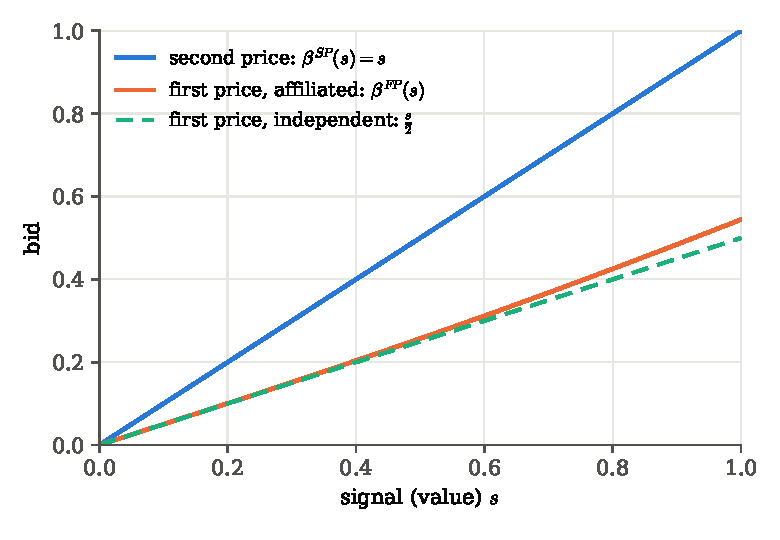
\includegraphics[width=0.72\textwidth]{figures/ch14/apv_bids.pdf}
  \caption{Equilibrium bids for the affiliated private values density $f(s_1,s_2)=\frac{4}{5}(1+s_1s_2)$ on
  $[0,1]^2$ with two bidders. The second-price bid is $s$. The first-price bid is \eqref{eq:14-apv-fpa}. The
  dashed line is the first-price bid $\frac{s}{2}$ for independent uniform values.}\label{fig:14-apv-bids}
\end{figure}

The first-order condition can also be written in terms of the bid distribution, which is the form used for
estimation. Consider affiliated private values, possibly asymmetric, and let $M_i=\max_{j\ne i}B_j$ be the
highest rival bid. Bidder $i$ with value $v_i$ solves
\begin{equation*}
  \max_b\ \E\left[(v_i-b)\indic\{M_i\le b\}\mid V_i=v_i\right]=\max_b\ (v_i-b)\Pr\left(M_i\le b\mid V_i=v_i\right).
\end{equation*}
The conditioning on $v_i$ matters, because under affiliation a bidder's own value is informative about rivals'
values and hence about their bids. The first-order condition is
\begin{equation*}
  -\Pr\left(M_i\le b\mid V_i=v_i\right)+(v_i-b)\frac{\partial\Pr\left(M_i\le b\mid V_i=v_i\right)}{\partial b}=0,
\end{equation*}
which rearranges to
\begin{equation*}
  v_i=b+\frac{\Pr\left(M_i\le b\mid V_i=v_i\right)}{\frac{\partial}{\partial b}\Pr\left(M_i\le b\mid V_i=v_i\right)}.
\end{equation*}
The derivative is taken in the threshold $b$, holding the conditioning value fixed. In an equilibrium with
strictly increasing strategies $\beta_i$, the events $\{V_i=v_i\}$ and $\{B_i=\beta_i(v_i)\}$ coincide. So
$\Pr(M_i\le m\mid V_i=v_i)=G_{M\mid B}(m\mid b_i)$, where $G_{M\mid B}(m\mid b)=\Pr(M_i\le m\mid B_i=b)$ and
$b_i=\beta_i(v_i)$. Let $g_{M\mid B}(m\mid b)$ be its density in $m$. At the equilibrium bid,
\begin{equation}\label{eq:14-apv-foc}
  v_i=b_i+\frac{G_{M\mid B}(b_i\mid b_i)}{g_{M\mid B}(b_i\mid b_i)}.
\end{equation}
Everything on the right side is a feature of the joint distribution of a bidder's own bid and the highest
rival bid, which is observed when all bids are recorded. \Cref{ch:auction-empirics} uses \eqref{eq:14-apv-foc}
to recover values from bids \citep{LiPerrigneVuong2002,CampoPerrigneVuong2003}. With common values the same
argument gives \citet[eq.~(2.4)]{AtheyHaile2007}, in which the left side is the pivotal expected value
$\E[V_i\mid S_i=s_i,\ M_i=\beta(s_i)]$. In the symmetric Milgrom-Weber model this is $v(s,s)$. There,
$G_{M\mid B}(b\mid b)=F_{Y_1}(s\mid s)$ and $g_{M\mid B}(b\mid b)=\frac{f_{Y_1}(s\mid s)}{\beta'(s)}$ at
$b=\beta(s)$, and \eqref{eq:14-apv-foc} becomes \eqref{eq:14-mw-ode}.

Existence and uniqueness of equilibrium are now well understood. The following theorem collects the results
summarized by \citet[Theorem~2.1]{AtheyHaile2007}.

\begin{theorem}[Existence and uniqueness in first-price auctions]\label{thm:14-existence}
Suppose values have a compact, convex common support, signals are affiliated with a product support, and
their joint density is strictly positive on the interior of the support.
\begin{enumerate}[label=(\roman*)]
  \item An equilibrium in pure, nondecreasing strategies exists \citep{Athey2001,RenyZamir2004}. Strategies
  can be taken strictly increasing, except in common values models with asymmetric bidders and dependent
  signals. There, at most one bidder may bid the lowest winning bid with positive probability
  \citep{McAdams2003}.
  \item With private values and either independence or symmetry, and a continuously differentiable density,
  the equilibrium is unique and in pure, strictly increasing, differentiable strategies
  \citep{Lebrun1999,MaskinRiley2003,McAdams2003,McAdams2007}.
  \item With symmetric bidders and a continuously differentiable density, there is a unique equilibrium
  within the class of nondecreasing pure strategies. It is symmetric, strictly increasing and differentiable,
  and it is the equilibrium of \cref{prop:14-mw-fpa} \citep{McAdams2007}.
\end{enumerate}
\end{theorem}

We do not prove the theorem. Existence for asymmetric bidders rests on single-crossing arguments that go
beyond this book. Part (iii) shows that, among monotone equilibria, the Milgrom-Weber first-price
equilibrium is the only one in the symmetric model.

\section{Affiliated Values II: The Linkage Principle, Revenue Ranking, and Information Disclosure}\label{sec:14-mw-rank}

With independent private values the four standard formats raise the same expected revenue
(\cref{prop:14-ret}). Affiliation breaks this equivalence in a systematic direction. This section explains why
through the linkage principle, proves the ranking, and applies the same logic to the seller's disclosure of
information, reserve prices and entry fees. It then asks which results survive risk aversion and closes with
an assessment of the paper.

\subsection{The linkage principle}\label{sec:14-linkage}

\citet[pp.~1110--1111]{MilgromWeber1982} view each auction as a revelation game in which every bidder chooses a
report $x$ in place of a bid $\beta(x)$. No auction can set prices directly in terms of bidders' preferences
and information. Prices can depend only on the reports and on the seller's information. If the price depends
on variables other than the winner's own report, and those variables are affiliated with the winner's signal,
then the price is statistically linked to that signal. The expected price, as a function of the winner's
signal, rises more steeply than it otherwise would. In all three auctions the winner with the lowest signal
expects to pay $v(\underline s,\underline s)$. A steeper expected payment function therefore means higher
prices and lower bidder profits.

To make this precise, consider a symmetric auction mechanism $\mathcal M$ with a symmetric, increasing
equilibrium in which the highest signal wins. For bidder 1 with signal $z$ who bids as if its signal were $x$,
define the expected value it receives,
\begin{equation*}
  R(x,z)=\E\left[V_1\indic\{Y_1<x\}\mid S_1=z\right],
\end{equation*}
and its expected payment conditional on winning, $W^{\mathcal M}(x,z)$. Its expected payoff is
$R(x,z)-W^{\mathcal M}(x,z)F_{Y_1}(x\mid z)$. In equilibrium $x=z$ is optimal, so the first-order condition
holds at $x=z$ \citep[eq.~(9)]{MilgromWeber1982}:
\begin{equation}\label{eq:14-mw-foc9}
  0=R_1(z,z)-W^{\mathcal M}_1(z,z)F_{Y_1}(z\mid z)-W^{\mathcal M}(z,z)f_{Y_1}(z\mid z),
\end{equation}
where subscripts denote partial derivatives. The boundary condition is
$W^{\mathcal M}(\underline s,\underline s)=v(\underline s,\underline s)$. In the first-price auction the
winner pays its own bid, so $W^{FP}(x,z)=\beta^{FP}(x)$. In the second-price auction it pays the highest rival
bid, so $W^{SP}(x,z)=\E[v(Y_1,Y_1)\mid Y_1<x,\,S_1=z]$. The partial derivative $W_2^{\mathcal M}$ measures how
much the expected price depends on the winner's true signal when its report is held fixed. We call it the
\emph{linkage} of the mechanism.

\begin{proposition}[Linkage principle]\label{prop:14-linkage}
Let $\mathcal M$ and $\mathcal M'$ be two mechanisms as above that satisfy \eqref{eq:14-mw-foc9}. Suppose
$W^{\mathcal M}(\underline s,\underline s)=W^{\mathcal M'}(\underline s,\underline s)$ and
$W^{\mathcal M}_2(z,z)\ge W^{\mathcal M'}_2(z,z)$ for all $z$. Then $W^{\mathcal M}(z,z)\ge W^{\mathcal
M'}(z,z)$ for all $z$, and $\mathcal M$ yields an expected revenue at least as large as $\mathcal M'$.
\end{proposition}

\begin{proof}
Let $g(z)=W^{\mathcal M}(z,z)$ and $h(z)=W^{\mathcal M'}(z,z)$. Solving \eqref{eq:14-mw-foc9} for $W_1$ in
each mechanism and subtracting,
\begin{equation*}
  W^{\mathcal M}_1(z,z)-W^{\mathcal M'}_1(z,z)=-\left[g(z)-h(z)\right]\frac{f_{Y_1}(z\mid z)}{F_{Y_1}(z\mid z)}.
\end{equation*}
By the chain rule $g'(z)=W^{\mathcal M}_1(z,z)+W^{\mathcal M}_2(z,z)$, and similarly for $h$. Therefore
\begin{equation*}
  g'(z)-h'(z)=-\left[g(z)-h(z)\right]\frac{f_{Y_1}(z\mid z)}{F_{Y_1}(z\mid z)}
  +\left[W^{\mathcal M}_2(z,z)-W^{\mathcal M'}_2(z,z)\right].
\end{equation*}
If $g(z)<h(z)$, the first term is positive and the second is nonnegative, so $g'(z)\ge h'(z)$. Since
$g(\underline s)=h(\underline s)$, \cref{lem:14-crossing} gives $g\ge h$ everywhere. By symmetry each bidder
wins with probability $\frac{1}{n}$, so expected revenue is
$n\,\E[W(S_1,S_1)\indic\{S_1>Y_1\}]=\E[W(S_1,S_1)\mid S_1>Y_1]$, which is larger under $\mathcal M$.
\end{proof}

The principle explains where bidders' profits come from. A bidder earns a rent because the price cannot
depend on its private signal except through its own report. Every channel that makes the price track its
signal through other affiliated variables reduces that rent. General versions of the principle are in
\citet{Milgrom2004} and \citet[Chapter~7]{Krishna2010}.

\subsection{Revenue ranking}\label{sec:14-mw-ranking}

The ranking rests on one inequality, which also delivers the disclosure results of
\cref{sec:14-mw-disclosure}.

\begin{lemma}[Information raises the second-price expected price]\label{lem:14-mw-info}
Let $\bm Z$ be a random vector such that $(\bm Z,S_1,Y_1)$ are affiliated, and let
$w_{\bm Z}(s,y,\bm z)=\E[V_1\mid S_1=s,\,Y_1=y,\,\bm Z=\bm z]$ be nondecreasing. Then
\begin{equation*}
  \E\left[v(Y_1,Y_1)\mid S_1>Y_1\right]\le\E\left[w_{\bm Z}(Y_1,Y_1,\bm Z)\mid S_1>Y_1\right].
\end{equation*}
\end{lemma}

\begin{proof}
By the law of iterated expectations, for all $x$ and $y$,
\begin{equation*}
  v(x,y)=\E\left[\E[V_1\mid S_1,Y_1,\bm Z]\mid S_1=x,Y_1=y\right]=\E\left[w_{\bm Z}(x,y,\bm Z)\mid S_1=x,Y_1=y\right].
\end{equation*}
Now take $x>y$. Applying this identity at the point $(y,y)$ and then \cref{prop:14-affil-props}(iii) to the
nondecreasing function $w_{\bm Z}(y,y,\cdot)$,
\begin{equation*}
  v(y,y)=\E\left[w_{\bm Z}(y,y,\bm Z)\mid S_1=y,Y_1=y\right]\le\E\left[w_{\bm Z}(y,y,\bm Z)\mid S_1=x,Y_1=y\right].
\end{equation*}
Setting $y=Y_1$ and $x=S_1$ on the event $\{S_1>Y_1\}$ and taking expectations,
\begin{equation*}
  \E\left[v(Y_1,Y_1)\mid S_1>Y_1\right]\le\E\left[\E\left[w_{\bm Z}(Y_1,Y_1,\bm Z)\mid S_1,Y_1\right]\mid S_1>Y_1\right]
  =\E\left[w_{\bm Z}(Y_1,Y_1,\bm Z)\mid S_1>Y_1\right].\qedhere
\end{equation*}
\end{proof}

\begin{proposition}[{\citealp[Theorems~11 and 15]{MilgromWeber1982}}]\label{prop:14-mw-ranking}
Let \cref{ass:14-mw} hold, and consider the equilibria of
\cref{prop:14-mw-english,prop:14-mw-spa,prop:14-mw-fpa}. The expected price in the English auction is at least
that in the second-price auction. The expected price in the second-price auction is at least that in the
first-price and Dutch auctions.
\end{proposition}

\begin{proof}
\emph{Second price versus first price.} Both equilibria satisfy \eqref{eq:14-mw-foc9}, because $x=z$ is optimal in
each. In the first-price auction $W^{FP}(x,z)=\beta^{FP}(x)$ does not depend on $z$, so $W^{FP}_2=0$. In the
second-price auction $W^{SP}(x,z)=\E[v(Y_1,Y_1)\mid Y_1<x,S_1=z]$. Since $(S_1,Y_1)$ are affiliated, $v$ is
nondecreasing and the event $\{Y_1<x\}$ is an interval, \cref{prop:14-affil-props}(iii) shows that $W^{SP}$
is nondecreasing in $z$, so $W^{SP}_2\ge0$. Both mechanisms satisfy the boundary condition
$W(\underline s,\underline s)=v(\underline s,\underline s)$. \Cref{prop:14-linkage} gives
$W^{SP}(z,z)\ge W^{FP}(z,z)$ for all $z$, and the expected prices are $\E[W(S_1,S_1)\mid S_1>Y_1]$.

\emph{English versus second price.} When bidder 1 wins, it pays $\bar v(Y_1,Y_1,Y_2,\dots,Y_{n-1})$ in the English
auction (\cref{prop:14-mw-english}) and $v(Y_1,Y_1)$ in the second-price auction. Apply \cref{lem:14-mw-info}
with $\bm Z=(Y_2,\dots,Y_{n-1})$. Then $w_{\bm Z}=\bar v$, which is nondecreasing by \cref{cor:14-mw-v}, and
$(S_1,Y_1,\dots,Y_{n-1})$ are affiliated by \cref{prop:14-affil-props}(iv) and (ii).

\emph{Dutch versus first price.} The two are strategically equivalent (\cref{prop:14-dutch-fpa}).
\end{proof}

The English auction proceeds in two phases \citep[p.~1105]{MilgromWeber1982}. In the first, the $n-2$
bidders with the lowest signals reveal them publicly by dropping out. In the second, the last two bidders play
what amounts to a second-price auction with this public information. \Cref{lem:14-mw-info} says that public
information affiliated with the bidders' signals raises the expected second-price price. The first phase
therefore raises the expected price above the second-price level. In the language of linkage, the English
price is linked to the signals of all losing bidders. The second-price price is linked only to the highest
losing signal, and the first-price price to no other signal at all.

\begin{figure}[htbp]
  \centering
  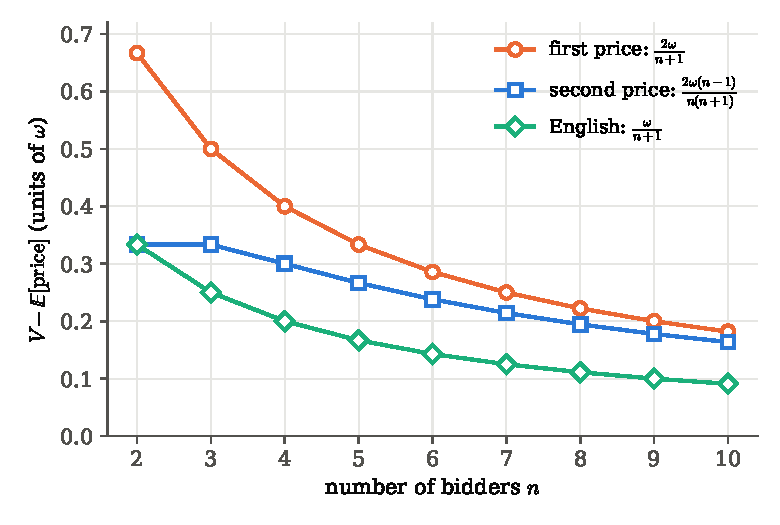
\includegraphics[width=0.72\textwidth]{figures/ch14/mw_mineral_rents.pdf}
  \caption{Expected bidder rents $V-\E[\text{price}]$, in units of $\omega$, in the mineral rights model with
  uniform noise (\cref{ex:14-mineral}) and a diffuse prior. The formulas are derived in the text, and a
  Monte Carlo check is in \texttt{mineral\_rights.py}.}\label{fig:14-mw-ranking}
\end{figure}

The mineral rights example (\cref{ex:14-mineral,ex:14-mineral-english,ex:14-mineral-fpa}) makes the ranking
explicit. Write $S_i=V+\omega(2U_i-1)$ with $U_i$ \iid\ uniform on $[0,1]$. The $k$-th lowest of $n$ uniforms
has mean $\frac{k}{n+1}$, so the $k$-th lowest signal has mean
\begin{equation*}
  \E\left[S_{(k:n)}\right]=V+\omega\left(\frac{2k}{n+1}-1\right)=V+\omega\,\frac{2k-n-1}{n+1}.
\end{equation*}
The first-price winner pays $S_{(n:n)}-\omega$, by \eqref{eq:14-mineral-fpa}. Its expected payment is
\begin{equation*}
  V+\omega\,\frac{n-1}{n+1}-\omega=V-\frac{2\omega}{n+1}.
\end{equation*}
The second-price winner pays $v(S_{(n-1:n)},S_{(n-1:n)})=S_{(n-1:n)}-\omega\frac{n-2}{n}$, by
\eqref{eq:14-mineral-spa}. Its expected payment is
\begin{equation*}
  V+\omega\,\frac{n-3}{n+1}-\omega\,\frac{n-2}{n}
  =V+\omega\,\frac{n(n-3)-(n-2)(n+1)}{n(n+1)}
  =V-\frac{2\omega(n-1)}{n(n+1)}.
\end{equation*}
The English winner pays $\frac{S_{(n-1:n)}+S_{(1:n)}}{2}$, with expectation
\begin{equation*}
  V+\frac{\omega}{2}\left(\frac{n-3}{n+1}+\frac{1-n}{n+1}\right)=V-\frac{\omega}{n+1}.
\end{equation*}
The expected bidder rents are therefore $\frac{2\omega}{n+1}$, $\frac{2\omega(n-1)}{n(n+1)}$ and
$\frac{\omega}{n+1}$. They are ranked as \cref{prop:14-mw-ranking} predicts, because $1\ge\frac{n-1}{n}$ and
$2(n-1)\ge n$. The English and second-price auctions tie at $n=2$, as they must. \Cref{fig:14-mw-ranking}
plots the rents. The first-price rent is twice the English rent for every $n$.

The affiliated private values example (\cref{ex:14-apv,ex:14-apv-fpa}) shows that interdependent values are
not needed. The second-price (and English) revenue is $\E[\min\{S_1,S_2\}]$. By symmetry,
\begin{equation*}
  \E[\min\{S_1,S_2\}]=2\int_0^1\int_0^{s_1}s_2\,\frac{4}{5}(1+s_1s_2)\,ds_2\,ds_1
  =\frac{8}{5}\int_0^1\left(\frac{s_1^2}{2}+\frac{s_1^4}{3}\right)ds_1=\frac{8}{5}\cdot\frac{7}{30}=\frac{28}{75}
  \approx0.3733.
\end{equation*}
We compute the first-price revenue $\E[\beta^{FP}(\max\{S_1,S_2\})]$ by numerical integration and obtain
$0.3676$. The gap is small because the correlation is only $0.054$, but its sign is the one the theory
predicts. Compare \cref{ex:14-iv-independent}, which has interdependent values $V=\frac{S_1+S_2}{2}$
and independent uniform signals. There both formats raise $\frac{1}{3}$. The ranking comes from the
affiliation of the signals. Interdependence of values alone does not produce it. \Cref{tab:14-mw-examples}
collects the numbers.

\begin{table}[htbp]
  \centering
  \caption{Equilibrium bids and expected revenue in the two running examples}\label{tab:14-mw-examples}
  \small
  \renewcommand{\arraystretch}{1.35}
  \begin{tabularx}{\textwidth}{@{}lXcc@{}}
    \toprule
    \multicolumn{4}{@{}l}{\textit{Panel A. Mineral rights with uniform noise, diffuse prior}}\\
    \midrule
    Format & Bid or price & $V-\E[\text{price}]$ & $n=3$\\
    \midrule
    First price & bid $s-\omega$ & $\frac{2\omega}{n+1}$ & $0.500\omega$\\[2pt]
    Second price & bid $s-\omega\frac{n-2}{n}$ & $\frac{2\omega(n-1)}{n(n+1)}$ & $0.333\omega$\\[2pt]
    English & price $\frac{Y_1+Y_{n-1}}{2}$ & $\frac{\omega}{n+1}$ & $0.250\omega$\\[2pt]
    Second price, $S_0$ disclosed & bid $w(s,s,s_0)$ & numerical & $0.192\omega$\\[2pt]
    English, $S_0$ disclosed & price $\frac{\max\{Y_1,S_0\}+\min\{Y_{n-1},S_0\}}{2}$ &
      $\frac{n\omega}{(n+1)(n+2)}$ & $0.150\omega$\\
    \midrule
    \multicolumn{4}{@{}l}{\textit{Panel B. Affiliated private values, $f(s_1,s_2)=\frac{4}{5}(1+s_1s_2)$, $n=2$}}\\
    \midrule
    Format & Bid & Revenue & Bidder surplus\\
    \midrule
    First price & \eqref{eq:14-apv-fpa} & $0.3676$ & $0.3257$\\
    Second price, English & $s$ & $\frac{28}{75}\approx0.3733$ & $0.3200$\\
    Independent uniform values & $\frac{s}{2}$ (first), $s$ (second) & $\frac{1}{3}$ & $\frac{1}{3}$\\
    \bottomrule
  \end{tabularx}

  \smallskip
  \begin{minipage}{\textwidth}
  \footnotesize Notes: In Panel A the seller's signal is $S_0=V+\epsilon_0$ with $\epsilon_0$ uniform on
  $[-\omega,\omega]$ and independent of the bidders' noise. The closed forms are derived in the text. The
  disclosed second-price rent is computed by numerical integration ($0.167\omega$, $0.192\omega$,
  $0.191\omega$ and $0.182\omega$ for $n=2,\dots,5$). In Panel B, expected total surplus is
  $\E[\max\{S_1,S_2\}]=\frac{52}{75}$ with affiliation and $\frac{2}{3}$ with independent uniform values.
  The first-price revenue is computed by numerical integration. Source: scripts \texttt{mineral\_rights.py}
  and \texttt{apv\_example.py}.
  \end{minipage}
\end{table}

\Cref{tab:14-mw-theorems} maps the paper's results to the places where this chapter states and proves them.

\begin{table}[htbp]
  \centering
  \caption{The results of Milgrom and Weber (1982) and where this chapter treats them}\label{tab:14-mw-theorems}
  \small
  \begin{tabularx}{\textwidth}{@{}lXl@{}}
    \toprule
    Result & Content & In this chapter\\
    \midrule
    Theorem 0 & Revenue equivalence with independent private values & \cref{prop:14-ret}\\
    Theorem 1 & Characterization of affiliation, products & \cref{prop:14-affil-char}\\
    Theorems 2--5 & Order statistics, monotone maps, marginals, conditional means & \cref{prop:14-affil-props}\\
    Lemma 1 & $\frac{F_{Y_1}(y\mid z)}{f_{Y_1}(y\mid z)}$ is nonincreasing in $z$ & \cref{lem:14-mw-lemma1}\\
    Theorem 6 & Second-price equilibrium $v(s,s)$ & \cref{prop:14-mw-spa}\\
    Theorem 7 & Garbled information earns nothing & \cref{prop:14-mw-garbling}\\
    Theorems 8, 12, 16 & Disclosure of $S_0$ raises second-price, English, first-price revenue &
      \cref{prop:14-mw-disclosure}\\
    Theorems 9, 13, 17 & No reporting policy beats full disclosure & \cref{prop:14-mw-fullreport}\\
    Theorem 10 & English equilibrium & \cref{prop:14-mw-english}\\
    Theorem 11 & English at least second price & \cref{prop:14-mw-ranking}\\
    Theorem 14 & First-price equilibrium & \cref{prop:14-mw-fpa}\\
    Lemma 2 & Crossing lemma & \cref{lem:14-crossing}\\
    Theorem 15 & Second price at least first price & \cref{prop:14-mw-ranking}\\
    Theorem 18 & Disclosure with an adjusted reserve price & \cref{prop:14-mw-reserve-info}\\
    Theorem 19 & Higher entry fee, lower reserve at a fixed screening level & \cref{prop:14-mw-fee}\\
    Theorem 20 & Information raises willingness to pay only under constant absolute risk aversion &
      \cref{prop:14-mw-cara}\\
    Theorem 21 & Disclosure and ranking under constant absolute risk aversion & \cref{prop:14-mw-cara-disclosure}\\
    Theorems 22--24 & Association and the general definition of affiliation & \cref{sec:14-mw-affil}\\
    \bottomrule
  \end{tabularx}
\end{table}

\subsection{Information disclosure by the seller}\label{sec:14-mw-disclosure}

Suppose the seller observes a variable $S_0$ that is affiliated with $(\bm A,\bm S)$, such as an expert
appraisal. Can the seller gain by revealing it? We assume that the seller can commit to a reporting policy and that its
reports are credible. Credibility is plausible if a buyer has recourse after a false announcement,
or if the seller is an institution, such as an auction house, that values its reputation for truthfulness
\citep[footnote~18]{MilgromWeber1982}.

Define $w(s,y,s_0)=\E[V_1\mid S_1=s,\,Y_1=y,\,S_0=s_0]$, which is nondecreasing by
\cref{prop:14-affil-props}(iii). After $S_0=s_0$ is announced, the conditional density of $(\bm A,\bm S)$ given
$s_0$ is proportional to $f(\bm a,\bm s,s_0)$ with $s_0$ held fixed. It satisfies \eqref{eq:14-affil-ineq}, since
the inequality for $f$ holds in particular for pairs of points with the same value of $s_0$. So the analysis of
\cref{sec:14-mw-eq} applies conditionally. In the second-price auction the equilibrium bid becomes
$\beta^{SP}(s;s_0)=w(s,s,s_0)$, a function of both private and public information
\citep[p.~1102]{MilgromWeber1982}.

\begin{proposition}[{\citealp[Theorems~8, 12 and 16]{MilgromWeber1982}}]\label{prop:14-mw-disclosure}
Let \cref{ass:14-mw} hold, and let $S_0$ be affiliated with $(\bm A,\bm S)$.
\begin{enumerate}[label=(\roman*)]
  \item In the second-price auction, the expected price without disclosure,
  $\mathcal R^{SP}_N=\E[v(Y_1,Y_1)\mid S_1>Y_1]$, is at most the expected price with public disclosure of
  $S_0$, $\mathcal R^{SP}_I=\E[w(Y_1,Y_1,S_0)\mid S_1>Y_1]$.
  \item In the English auction, the expected price without disclosure,
  $\mathcal R^E_N=\E[\bar v(Y_1,Y_1,Y_2,\dots,Y_{n-1})\mid S_1>Y_1]$, is at most the expected price with
  disclosure, $\mathcal R^E_I=\E[\bar w(Y_1,Y_1,Y_2,\dots,Y_{n-1},S_0)\mid S_1>Y_1]$, where
  $\bar w(s,y_1,\dots,y_{n-1},s_0)=\E[V_1\mid S_1=s,\,Y_1=y_1,\dots,Y_{n-1}=y_{n-1},\,S_0=s_0]$.
  \item In the first-price auction, public disclosure of $S_0$ cannot lower, and may raise, the expected price.
\end{enumerate}
\end{proposition}

\begin{proof}
\emph{Part (i).} By symmetry the expected price equals the expected price paid by bidder 1 when it wins, which is
$v(Y_1,Y_1)$ without disclosure and $w(Y_1,Y_1,S_0)$ with it. Apply \cref{lem:14-mw-info} with $\bm Z=S_0$.
The vector $(S_0,S_1,Y_1)$ is affiliated by \cref{prop:14-affil-props}(iv) and (ii), with $S_0$ counted
among the variables $\bm A$, and $w$ is nondecreasing.

\emph{Part (ii).} The argument of \cref{lem:14-mw-info} goes through with $(Y_2,\dots,Y_{n-1})$ added to every
conditioning set. For $x>y_1$,
\begin{align*}
  \bar v(y_1,y_1,y_2,\dots,y_{n-1})
  &=\E\left[\bar w(y_1,y_1,\dots,y_{n-1},S_0)\mid S_1=y_1,Y_1=y_1,\dots\right]\\
  &\le\E\left[\bar w(y_1,y_1,\dots,y_{n-1},S_0)\mid S_1=x,Y_1=y_1,\dots\right],
\end{align*}
where the dots stand for $Y_2=y_2,\dots,Y_{n-1}=y_{n-1}$. Taking expectations over $\{S_1>Y_1\}$ gives the
result.

\emph{Part (iii), sketch.} Let $\beta(\cdot;s_0)$ be the first-price equilibrium after $S_0=s_0$ is announced. It
solves the analogue of \eqref{eq:14-mw-ode} with $w(s,s,s_0)$ in place of $v(s,s)$ and the ratio
$\zeta(s;s_0)=\frac{f_{Y_1}(s\mid s,s_0)}{F_{Y_1}(s\mid s,s_0)}$, with boundary value
$w(\underline s,\underline s,s_0)$. A variant of \cref{lem:14-mw-lemma1} shows that $\zeta(s;s_0)$ is
nondecreasing in $s_0$, and $w$ is nondecreasing in $s_0$. For $s_0'>s_0$, let $g=\beta(\cdot;s_0')$ and
$h=\beta(\cdot;s_0)$. Then $g(\underline s)\ge h(\underline s)$, and $g(x)<h(x)$ implies
$g'(x)=(w(x,x,s_0')-g(x))\zeta(x;s_0')\ge(w(x,x,s_0)-h(x))\zeta(x;s_0)=h'(x)$. By
\cref{lem:14-crossing}, $\beta(x;s_0)$ is nondecreasing in $s_0$. Now define
$W^*(x,z)=\E[\beta(x;S_0)\mid Y_1<x,\,S_1=z]$, the expected payment of a winner with signal $z$ who bids as
if $x$ whatever $S_0$ turns out to be. By \cref{prop:14-affil-props}(iii), $W^*_2\ge0=W^{FP}_2$. The boundary
value is $W^*(\underline s,\underline s)=\E[w(\underline s,\underline s,S_0)\mid Y_1=S_1=\underline s]
=v(\underline s,\underline s)$. A bidder who commits to the report $x$ before $S_0$ is announced chooses
$x=z$, because $x=z$ is optimal for every realization of $S_0$. So $W^*$ satisfies \eqref{eq:14-mw-foc9}.
\Cref{prop:14-linkage} gives $W^*(z,z)\ge\beta^{FP}(z)$, and the expected price is higher with
disclosure.
\end{proof}

Could the seller do better by censoring, that is, reporting $S_0$ only when it is favorable? No. If the policy
is known, rational bidders interpret the absence of a report as bad news. More generally, let the seller's
report be $S_0'=\varrho(S_0,Z)$, where $Z$ is uniform on $[0,1]$ and independent of everything else. The
report may depend both on the seller's information and on the spin of a roulette wheel. Since the policy is
known, we can assume without loss that the seller always makes some report, possibly a blank page
\citep[p.~1103]{MilgromWeber1982}.

\begin{proposition}[{\citealp[Theorems~9, 13 and 17]{MilgromWeber1982}}]\label{prop:14-mw-fullreport}
In the second-price, English and first-price auctions, no reporting policy yields a higher expected price
than always reporting $S_0$.
\end{proposition}

\begin{proof}
Let $g(s_0'\mid s_0)$ be the conditional density of the report given $S_0$ and $g(s_0')$ its marginal. Given
$S_0'=s_0'$, the conditional density of $(\bm A,\bm S,S_0)$ is
$\frac{f(\bm a,\bm s,s_0)\,g(s_0'\mid s_0)}{g(s_0')}$ \citep[footnote~19]{MilgromWeber1982}. For fixed
$s_0'$, this is the product of the affiliated density $f$ and a nonnegative function of $s_0$ alone. A function
of one variable satisfies \eqref{eq:14-affil-ineq} with equality, so the product is affiliated by
\cref{prop:14-affil-char}. Conditional on $S_0'=s_0'$, \cref{prop:14-mw-disclosure} therefore says that
revealing $S_0$ as well raises the expected price. Revealing both $S_0$ and $S_0'$ leads to the same bidding as
revealing $S_0$ alone, because $S_0'$ carries no information about $(\bm A,\bm S)$ beyond $S_0$. Averaging over
$S_0'$ completes the proof.
\end{proof}

Full disclosure links the price to $S_0$, a variable affiliated with the winner's signal that the winner
cannot influence. It dilutes the winner's informational advantage and so lowers its rent
\citep[p.~1117]{MilgromWeber1982}. The results offer an explanation for the expert appraisals and catalog
estimates that reputable auction houses publish.

The mineral rights example quantifies the effect (Panel A of \cref{tab:14-mw-examples}). Let the seller observe
$S_0=V+\epsilon_0$, with $\epsilon_0$ uniform on $[-\omega,\omega]$ and independent of the bidders' noise. In
the English auction with $S_0$ public, the posterior of $V$ at the last exit is uniform. Its support runs from
the largest signal minus $\omega$ to the smallest signal plus $\omega$, where $S_0$ now counts as a signal.
The winner pays
$\frac{\max\{Y_1,S_0\}+\min\{Y_{n-1},S_0\}}{2}$. In uniform units, $\min\{U_{(1:n)},U_0\}$ is the minimum of
$n+1$ uniforms, with mean $\frac{1}{n+2}$. The maximum $\max\{U_{(n-1:n)},U_0\}$ has distribution function
$x\Lambda_n(x)$, where $\Lambda_n(x)=nx^{n-1}(1-x)+x^n$ is the distribution function of $U_{(n-1:n)}$. Its
mean is
\begin{equation*}
  1-\int_0^1x\Lambda_n(x)\,dx=1-n\left(\frac{1}{n+1}-\frac{1}{n+2}\right)-\frac{1}{n+2}
  =1-\frac{2n+1}{(n+1)(n+2)}.
\end{equation*}
Converting back with $S=V+\omega(2U-1)$, the price is
\begin{equation*}
  V+\omega\left(\max\{U_{(n-1:n)},U_0\}+\min\{U_{(1:n)},U_0\}-1\right),
\end{equation*}
so the expected rent is
\begin{equation*}
  V-\E[\text{price}]=\omega\left[\frac{2n+1}{(n+1)(n+2)}-\frac{1}{n+2}\right]=\frac{n\omega}{(n+1)(n+2)}.
\end{equation*}
Disclosure multiplies the English rent $\frac{\omega}{n+1}$ by $\frac{n}{n+2}$. For $n=2$ it halves the
rent, from $\frac{\omega}{3}$ to $\frac{\omega}{6}$. In the second-price auction the price becomes
$w(Y_1,Y_1,S_0)$, the mean of a density proportional to $(Y_1+\omega-V)^{n-2}$ on
$[\max\{Y_1,S_0\}-\omega,\ \min\{Y_1,S_0\}+\omega]$. Numerical integration gives a rent of $0.192\omega$ for
$n=3$, against $0.333\omega$ without disclosure.

\subsection{Reserve prices and entry fees}\label{sec:14-mw-reserve}

So far no reserve price or entry fee has played a role. Bids were restricted to be nonnegative, which amounts
to a reserve price of zero that never binds, because values are nonnegative
\citep[footnote~25]{MilgromWeber1982}. Without any reserve, other symmetric equilibria can appear, as
\cref{sec:14-fpa} shows for uniform private values.

A reserve price $r$ above $v(\underline s,\underline s)$ changes the analysis in one way. Only bidders whose
signals exceed a \emph{screening level} participate, where \citep[eq.~(10)]{MilgromWeber1982}
\begin{equation}\label{eq:14-mw-screen}
  s^*(r)=\inf\left\{s:\ \E\left[V_1\mid S_1=s,\ Y_1<s\right]\ge r\right\}.
\end{equation}
The marginal participant wins only when every rival's signal lies below $s^*$, so that no rival bids, and then
it pays $r$. It must therefore be indifferent between participating and staying out, which is the condition
$\E[V_1\mid S_1=s^*,Y_1<s^*]=r$. The conditional mean is nondecreasing in $s$ by
\cref{prop:14-affil-props}(iii), so the screening level rises with $r$.

The equilibrium strategies adapt in a simple way \citep[p.~1111]{MilgromWeber1982}. In the first-price
auction the bid solves \eqref{eq:14-mw-ode} on $[s^*,\bar s]$ with boundary condition $\beta(s^*)=r$. Repeating
the integrating-factor argument from $s^*$ in place of $\underline s$,
\begin{equation*}
  \beta^{FP}(s)=r\,L(s^*\mid s)+\int_{s^*}^sv(\alpha,\alpha)\,dL(\alpha\mid s)\quad\text{for }s\ge s^*,
\end{equation*}
and types below $s^*$ bid less than $r$ or not at all. In the second-price auction the bid is $v(s,s)$ for
$s\ge s^*$, and types below $s^*$ do not bid. When at least two bidders participate, the winner pays the
highest rival bid. A sole participant pays $r$. The marginal type's expected payoff is
$F_{Y_1}(s^*\mid s^*)\left(\E[V_1\mid S_1=s^*,Y_1<s^*]-r\right)=0$, so the same screening level
applies. The same set of bidders participates in all three auctions with the same reserve price. The revenue
ranking of \cref{prop:14-mw-ranking} survives a fixed reserve price \citep[p.~1112]{MilgromWeber1982}.

The second-price auction with a reserve has a curious feature \citep[footnote~26]{MilgromWeber1982}. By
\cref{prop:14-wc}, $v(s^*,s^*)\ge\E[V_1\mid S_1=s^*,Y_1<s^*]=r$. When the inequality is strict, bids jump from
nothing below $s^*$ to $v(s^*,s^*)>r$ at $s^*$, so no bids fall in a neighborhood above $r$. The marginal
participant bids above the reserve because winning against a participating rival is better news than winning
alone.

Seller information interacts with the reserve price. If the seller fixes a reserve price and then reveals
$S_0$, the revelation changes the screening level and hence the set of competitors. Favorable news attracts
bidders and unfavorable news deters them. The seller can offset this by adjusting the reserve to the
announcement. Fix a reserve $\bar r$ and let $s^*(r\mid s_0)$ be the screening level when $S_0=s_0$ is
announced and the reserve is $r$. It is nondecreasing in $r$ and nonincreasing in $s_0$. Let $r(s_0\mid\bar r)$
be the reserve that keeps the screening level fixed, so that $s^*(r(s_0\mid\bar r)\mid s_0)=s^*(\bar r)$.

\begin{proposition}[{\citealp[Theorem~18]{MilgromWeber1982}}]\label{prop:14-mw-reserve-info}
For any reserve price $\bar r$ in the first-price, second-price or English auction, announcing $S_0$ and
setting the reserve $r(S_0\mid\bar r)$ raises the expected price.
\end{proposition}

\begin{proof}[Proof for the second-price auction]
Let $s^*=s^*(\bar r)$ and $Y_1^*=\max\{Y_1,s^*\}$. Define $v^*(x,y)=\E[V_1\mid S_1=x,Y^*_1=y]$ and
$w^*(x,y,s_0)=\E[V_1\mid S_1=x,Y^*_1=y,S_0=s_0]$. Bidder 1 wins exactly when $S_1>Y_1^*$. Without disclosure
it then pays $v(Y_1,Y_1)$ if $Y_1\ge s^*$ and $\bar r$ if $Y_1<s^*$. Both cases equal $v^*(Y^*_1,Y^*_1)$,
because $\bar r=\E[V_1\mid S_1=s^*,Y_1<s^*]=v^*(s^*,s^*)$ by \eqref{eq:14-mw-screen}. With disclosure and the
adjusted reserve it pays $w(Y_1,Y_1,S_0)$ or $r(S_0\mid\bar r)=\E[V_1\mid S_1=s^*,Y_1<s^*,S_0]$, which both
equal $w^*(Y_1^*,Y_1^*,S_0)$. The map $Y_1\mapsto\max\{Y_1,s^*\}$ is nondecreasing, so $(S_0,S_1,Y_1^*)$ are
affiliated by \cref{prop:14-affil-props}(i), and $v^*,w^*$ are nondecreasing. The argument of
\cref{lem:14-mw-info}, with $Y^*_1$ in place of $Y_1$, then gives $\E[v^*(Y_1^*,Y_1^*)\mid S_1>Y_1^*]\le
\E[w^*(Y_1^*,Y_1^*,S_0)\mid S_1>Y_1^*]$. The English case is the same with $Y_2,\dots,Y_{n-1}$ added, and the
first-price case adapts the argument of \cref{prop:14-mw-disclosure}(iii) \citep[p.~1112]{MilgromWeber1982}.
\end{proof}

As with \cref{prop:14-mw-fullreport}, no partial reporting policy beats full revelation with an adjusted
reserve.

Entry fees add a second instrument. With a reserve price $r$ and an entry fee $e$ paid by every participant,
the screening level becomes
\begin{equation*}
  s^*(r,e)=\inf\left\{s:\ \E\left[(V_1-r)\indic\{Y_1<s\}\mid S_1=s\right]\ge e\right\}.
\end{equation*}
The left side is the expected profit of the marginal participant, who wins only when nobody else enters and
then pays $r$. It need not be true that exactly the bidders above $s^*(r,e)$ choose to enter. In a first-price
auction, a bidder with a signal well above $s^*(r,e)$ may stay out if its chance of winning,
$F_{Y_1}(s\mid s)$, is small \citep[p.~1112]{MilgromWeber1982}.

\begin{definition}[Regular reserve price and entry fee]\label{def:14-regular-pair}
A reserve price and entry fee pair $(r,e)$ is \emph{regular} for an auction if, in equilibrium, the bidders who
participate are exactly those with signals above $s^*(r,e)$.
\end{definition}

A zero entry fee is always regular. \citet[footnote~27]{MilgromWeber1982} give an irregular pair. Let $n=2$
and $V_i=S_i$. With probability $\frac{1}{2}$ both signals are drawn independently and uniformly from $[0,2]$,
and with probability $\frac{1}{2}$ from $[1,2]$. Take $r=0$ and $e=0.32$. For $s<1$ only the first regime is
possible, $F_{Y_1}(s\mid s)=\frac{s}{2}$, and $s\cdot\frac{s}{2}=0.32$ gives $s^*=0.8$. Just above $s=1$, Bayes'
rule puts posterior probability $\frac{1}{3}$ on the first regime. Then $F_{Y_1}(s\mid s)$ drops from
$\frac{1}{2}$ to $\frac{1}{3}\cdot\frac{1}{2}=\frac{1}{6}$ (the printed footnote reports $\frac{1}{4}$, and the
conclusion is the same). A bidder with $s$ slightly above 1 expects a gross payoff of at most
$sF_{Y_1}(s\mid s)\approx\frac{1}{6}<0.32$, so it stays out although its value exceeds $s^*$.

\begin{proposition}[{\citealp[Theorem~19]{MilgromWeber1982}}]\label{prop:14-mw-fee}
Fix the first-price, second-price or English auction, and let $(r,e)$ be regular. Let $(\tilde r,\tilde e)$
have the same screening level, $s^*(r,e)=s^*(\tilde r,\tilde e)$, and $\tilde e<e$. Then $(\tilde r,\tilde e)$
is regular, and its expected revenue is at most that of $(r,e)$.
\end{proposition}

\begin{proof}[Sketch]
Let $P(x,z)$ and $\tilde P(x,z)$ be bidder 1's expected payments (not conditional on winning) under the two
pairs when its signal is $z$ and it bids as if $x$. With $R$ as in \cref{sec:14-linkage}, the equilibrium
conditions are $P_1(z,z)=R_1(z,z)=\tilde P_1(z,z)$ for $z\ge s^*$ and $P(s^*,s^*)=R(s^*,s^*)=\tilde
P(s^*,s^*)$. Since $\tilde e<e$ at the same screening level, $\tilde r>r$. In the first-price auction,
$P(x,z)=b(x)F_{Y_1}(x\mid z)+e$ and $\tilde P(x,z)=\tilde b(x)F_{Y_1}(x\mid z)+\tilde e$, where $b$ and
$\tilde b$ solve the same differential equation with $b(s^*)=r<\tilde r=\tilde b(s^*)$. Solutions of a
first-order equation cannot cross, so $b<\tilde b$ everywhere. Hence
\begin{equation*}
  P_2(x,x)-\tilde P_2(x,x)=\left[b(x)-\tilde b(x)\right]\frac{\partial F_{Y_1}(x\mid z)}{\partial z}\Big|_{z=x}\ge0,
\end{equation*}
because affiliation makes $F_{Y_1}(x\mid z)$ nonincreasing in $z$. In the second-price and English auctions the
payments differ only when the bidder pays the reserve price, that is, when $Y_1<s^*$. Then
$P_2(x,z)-\tilde P_2(x,z)=(r-\tilde r)\frac{\partial F_{Y_1}(s^*\mid z)}{\partial z}\ge0$. In each case the
argument of \cref{prop:14-linkage}, built on \cref{lem:14-crossing}, gives $P(z,z)\ge\tilde P(z,z)$ for all
$z\ge s^*$. Participants therefore pay more on average under $(r,e)$. Under $(\tilde r,\tilde e)$ they earn
$R(z,z)-\tilde P(z,z)\ge R(z,z)-P(z,z)\ge0$ and so participate. Types below $s^*$ still prefer to stay out,
which uses the quasiconcavity of the bidder's problem and affiliation once more
\citep[pp.~1113--1114]{MilgromWeber1982}.
\end{proof}

The intuition is again linkage. An entry fee is paid whatever the bidder's signal. The reserve price is paid
only when nobody else participates, an event whose probability $F_{Y_1}(s^*\mid z)$ falls as the bidder's
signal rises. Replacing reserve-price revenue with entry-fee revenue removes this negative link between the
payment and the bidder's signal. It makes the expected payment rise more steeply with the signal, which lowers
bidders' rents.

\subsection{Risk aversion}\label{sec:14-mw-risk}

With independent private values and risk-averse bidders, the first-price auction raises more expected revenue
than the second-price auction (\cref{prop:14-risk-fpa}). In Milgrom and Weber's version of the argument
\citep[eq.~(11)]{MilgromWeber1982}, a risk-averse bidder's first-price bid function rises at least as fast as
the risk-neutral one wherever it lies below it. The second-price bid is unaffected by risk aversion. Together
with \cref{prop:14-mw-ranking}, this has a sharp consequence. With both affiliation and risk aversion, the
first-price and second-price auctions cannot be ranked in general \citep[p.~1114]{MilgromWeber1982}.
Affiliation favors the second-price auction, and risk aversion favors the first-price auction.

Let bidders have a utility of money $\mathcal U$ that is increasing, concave and differentiable, with
$\mathcal U(0)=0$, and let reserve prices and entry fees be zero. The second-price analysis extends once
$v$ is redefined as a certainty equivalent. Let $v(x,y)$ solve
$\E\left[\mathcal U\left(V_1-v(x,y)\right)\mid S_1=x,Y_1=y\right]=\mathcal U(0)$. The proof of
\cref{prop:14-mw-spa} carries over, and $\beta^{SP}(x)=v(x,x)$ remains an equilibrium
\citep[p.~1115]{MilgromWeber1982}. Define $w(x,y,s_0)$ in the same way with $S_0=s_0$ added to the conditioning
set.

With risk neutrality, the disclosure results rest on the inequality
$\E[w(S_1,Y_1,S_0)\mid S_1,Y_1]\ge v(S_1,Y_1)$, which holds with equality. For risk-averse bidders the inequality
says that resolving uncertainty by releasing information lowers the risk premium that bidders demand. If the
information resolves all uncertainty, the premium falls to zero. Partial resolution need not lower it. To state
the issue formally, take a pair $(V,X)$ of a value and a signal. Define $\chi(x)$ by
$\E[\mathcal U(V-\chi(X))\mid X=x]=\mathcal U(0)$ and $\bar\chi$ by $\E[\mathcal U(V-\bar\chi)]=\mathcal
U(0)$. These are the willingness to pay with and without the information $X$. Revealing $X$ \emph{raises
average willingness to pay} if $\E[\chi(X)]\ge\bar\chi$.

\begin{proposition}[{\citealp[Theorem~20]{MilgromWeber1982}}]\label{prop:14-mw-cara}
Let $\mathcal U$ be increasing. Revealing $X$ raises average willingness to pay for every pair $(V,X)$ if and
only if the coefficient of absolute risk aversion $-\frac{\mathcal U''}{\mathcal U'}$ is a nonnegative
constant.
\end{proposition}

\begin{proof}[Proof of sufficiency and sketch of necessity]
\emph{Sufficiency.} Under risk neutrality the claim is immediate. Adding a constant to $\mathcal U$ does not change
$\chi$ or $\bar\chi$, so with constant absolute risk aversion $\kappa>0$ we may take
$\mathcal U(x)=-e^{-\kappa x}$, with $\mathcal U(0)=-1$. Factor the utility as
$\mathcal U(V-\bar\chi)=e^{\kappa(\bar\chi-\chi(X))}\,\mathcal U(V-\chi(X))$. Then
\begin{align*}
  \mathcal U(0)&=\E\left[\mathcal U(V-\bar\chi)\right]
  =\E\left[e^{\kappa(\bar\chi-\chi(X))}\,\E\left[\mathcal U(V-\chi(X))\mid X\right]\right]\\
  &=\E\left[e^{\kappa(\bar\chi-\chi(X))}\right]\mathcal U(0).
\end{align*}
Since $\mathcal U(0)\ne0$, $\E[e^{\kappa(\bar\chi-\chi(X))}]=1$. By Jensen's inequality,
$e^{\kappa(\bar\chi-\E[\chi(X)])}\le\E[e^{\kappa(\bar\chi-\chi(X))}]=1$, so $\bar\chi\le\E[\chi(X)]$.

\emph{Necessity, sketch.} Normalize $\mathcal U(0)=0$. Let $X$ take the values 0 and 1 with probability
$\frac{1}{2}$ each, let $V_a=X(Z+a)$, and let $Z$ be independent of $X$ with $\E[\mathcal U(Z)]=0$. Then
$\chi_a(0)=0$, $\chi_a(1)=a$ and $\E[\chi_a(X)]=\frac{a}{2}$. If revealing $X$ always raises willingness to pay,
then $\bar\chi_a\le\frac{a}{2}$. Since $\mathcal U$ is increasing,
\begin{equation*}
  0=\E\left[\mathcal U(V_a-\bar\chi_a)\right]=\frac{1}{2}\E\left[\mathcal U(Z+a-\bar\chi_a)\right]
  +\frac{1}{2}\mathcal U(-\bar\chi_a)
  \ge\frac{1}{2}\E\left[\mathcal U\left(Z+\frac{a}{2}\right)\right]+\frac{1}{2}\mathcal U\left(-\frac{a}{2}\right).
\end{equation*}
The last expression is zero at $a=0$, so it is maximized there, for every admissible $Z$. The first- and
second-order conditions give $\E[\mathcal U'(Z)]=\mathcal U'(0)$ and $\E[\mathcal U''(Z)]+\mathcal U''(0)\le0$.
Varying $Z$ shows that $\mathcal U'$ composed with $\mathcal U^{-1}$ must be affine, so
$\mathcal U'=c\,\mathcal U+\mathcal U'(0)$. The solutions are linear or exponential utilities, and the
second-order condition leaves only those with constant, nonnegative absolute risk aversion
\citep[pp.~1115--1116]{MilgromWeber1982}.
\end{proof}

\begin{proposition}[{\citealp[Theorem~21]{MilgromWeber1982}}]\label{prop:14-mw-cara-disclosure}
Suppose bidders are risk averse with constant absolute risk aversion.
\begin{enumerate}[label=(\roman*)]
  \item In the second-price and English auctions, public disclosure of $S_0$ raises the expected price.
  \item Among all reporting policies, full disclosure yields the highest expected price in these two auctions.
  \item The expected price in the English auction is at least that in the second-price auction.
\end{enumerate}
\end{proposition}

\begin{proof}[Proof of (i) for the second-price auction]
A corollary of \cref{prop:14-mw-cara}, applied conditionally on $S_1=x$ and $Y_1=y$, is
$\E[w(S_1,Y_1,S_0)\mid S_1=x,Y_1=y]\ge v(x,y)$. Since $w$ is nondecreasing, for all $x>y$,
\begin{align*}
  v(y,y)&\le\E\left[w(S_1,Y_1,S_0)\mid S_1=y,Y_1=y\right]
  =\E\left[w(Y_1,Y_1,S_0)\mid S_1=y,Y_1=y\right]\\
  &\le\E\left[w(Y_1,Y_1,S_0)\mid S_1=x,Y_1=y\right],
\end{align*}
where the last step uses \cref{prop:14-affil-props}(iii). Taking expectations over $\{S_1>Y_1\}$ gives
$\E[v(Y_1,Y_1)\mid S_1>Y_1]\le\E[w(Y_1,Y_1,S_0)\mid S_1>Y_1]$.
\end{proof}

The proof separates two effects of disclosure \citep[p.~1117]{MilgromWeber1982}. The second inequality is the
risk-neutral effect. Disclosure dilutes the winner's informational advantage and lowers its profit. The first
inequality is new. With constant absolute risk aversion, disclosure also raises bidders' average willingness
to pay. Milgrom and Weber argue that disclosure lowers average willingness to pay only when the range of
possible wealth outcomes is large and much uncertainty remains unresolved. They judge that combination unusual
for auction houses, so the result may account for the prevalence of English auctions and of published expert
appraisals.

\subsection{Assessment of Milgrom and Weber (1982)}\label{sec:14-mw-assessment}

\casehead{Contribution} The paper built one framework that nests the independent private values model and the
common value model, together with the intermediate cases that real auctions present. It identified affiliation
as the property that organizes the theory. Affiliation is weak enough to cover the leading examples and strong
enough to sign every comparison. With it, the paper derived equilibria in closed form for the second-price,
English and first-price auctions, and it ranked the formats by expected revenue. It explained two features of
practice that the private values theory could not, the prevalence of ascending auctions and sellers'
willingness to publish appraisals. The linkage principle gave a single intuition for all of these results.
\citet{Krishna2010} and \citet{Milgrom2004} build their textbook treatments of interdependent values on this
framework.

\casehead{Limitations and critiques} Symmetry is essential. With asymmetric bidders, equilibria lack closed
forms, the first-price auction can allocate inefficiently, and the revenue ranking can fail
(\cref{sec:14-asym} and \citealp{MaskinRiley2000}). Symmetry alone does not secure efficiency either. The
standard formats award the object to the highest signal, and with interdependent values that bidder need
not value the object most (\cref{tab:14-ranking}). The linkage principle need not extend to multi-unit auctions.
\citet{PerryReny1999} show by example that it can fail when bidders demand more than one unit.
Affiliation is a strong form of positive dependence. It requires the inequality \eqref{eq:14-affil-ineq} at
every pair of points and rules out negatively dependent signals. One-dimensional signals are a further
restriction \citep[footnote~14]{MilgromWeber1982}. In the English auction with common values the equilibrium
is not unique \citep{BikhchandaniHaileRiley2002}, so the revenue comparison selects one equilibrium among many.
Milgrom and Weber themselves list open problems in their Section 9 (pp.~1117--1118). Auctions in use account
for hundreds of billions of dollars of trade every year, yet the theory was still poorly developed. Bidding for
weapons systems is affected by expected renegotiation. The assumption that each auction can be studied in
isolation also fails at times. The Department of the Interior may offer about 200 oil tracts at once, and a
bidder on many tracts may worry about winning too many as well as too few. Examples by
\citet{EngelbrechtWiggansWeber1979} suggest that the optimal strategy may then place high bids on a few tracts
and low bids on several others of comparable value. Resale markets for drilling rights raise similar issues.
Lumber mill owners who bid repeatedly against each other for timber may collude, which raises the question of
which formats are least vulnerable (\cref{sec:14-collusion}). Their footnote~9 (p.~1090) adds that collusion had
received no attention in theoretical studies, despite many allegations of collusion in bidding for timber
rights \citep{Mead1967}. Milgrom and Weber treat bidding syndicates as a further collusion issue. They
ask why large oil companies sometimes bid jointly with smaller ones and how such syndicates affect prices. They also note that auctions for shares of a
divisible object had received relatively little attention \citep[p.~1118]{MilgromWeber1982}. Laboratory
evidence also qualifies the
rationality assumption. \citet{KagelLevin1986} find that subjects in common value auctions often fail to
correct fully for the winner's curse, especially in larger groups. Where bidders fall prey to the curse,
public information can lower revenue by helping them correct it, contrary to the theory's prediction.

\casehead{Empirical relevance} The model also delimits what auction data can reveal.
\citet[Section~7]{AtheyHaile2007} normalize signals so that $\E[V_i\mid S_i=\max_{j\ne i}S_j=s]=s$ (their
eq.~(7.1)). The first-price condition \eqref{eq:14-apv-foc} then states that $s_i=b_i+\frac{G_{M\mid B}(b_i\mid
b_i)}{g_{M\mid B}(b_i\mid b_i)}$ (their eq.~(7.2)). With common values, first-price bids identify only the
distribution of the pivotal values $v(S_i,S_i)$. With a fixed number of bidders and no reserve price, common
values and private values cannot be distinguished \citep{LaffontVuong1996,GuerrePerrigneVuong2000}. Ascending
auctions are harder still. In \citet[Theorem~7.1]{AtheyHaile2007}, three bidders have uniform signals and
either $V=\frac{S_1+S_2+S_3}{3}$ or $V=\frac{S_{(1:3)}}{3}+\frac{S_{(2:3)}}{6}+\frac{S_{(3:3)}}{2}$. The two
models produce the same distribution of exit prices in the Milgrom-Weber equilibrium, yet they imply different
optimal reserve prices. Progress requires more structure or more data. Variation in the number of bidders
allows tests of private against common values, and ex post measures of the value help in auctions of offshore
oil leases \citep{HendricksPorter1988,HendricksPinksePorter2003}. \Cref{ch:auction-empirics} develops these
approaches.

\section{Asymmetric Bidders}\label{sec:14-asym}

The models of \cref{sec:14-fpa,sec:14-mw-eq,sec:14-mw-rank} treat every bidder as a draw from the same
population, and the assessment in \cref{sec:14-mw-assessment} noted that symmetry is essential to the
Milgrom-Weber results. Many auctions instead pit different kinds of firms against each other. In the timber sales studied by
\citet{AtheyLevinSeira2011}, sawmills with their own manufacturing capacity compete with independent
loggers who must resell the timber. In public procurement, domestic firms compete with foreign firms,
and incumbents compete with entrants. This section develops the private values model with bidders
who draw their values from different distributions.

The mechanism-design results of \cref{sec:14-ret} already allow bidder-specific distributions.
Revenue equivalence therefore still holds for any two auctions that allocate the object in the same
way. Asymmetry matters because it makes the first-price auction allocate the object differently from
the second-price and ascending auctions. We show how the allocation changes, who gains and who loses,
and why the revenue comparison becomes ambiguous.

\subsection{The asymmetric private values model}\label{sec:14-asym-model}

\begin{assumption}[Asymmetric independent private values]\label{ass:14-asym}
There are $n\ge 2$ risk-neutral bidders, $i\in\mathcal N=\{1,\dots,n\}$. Bidder $i$'s value $V_i$ is
drawn from a distribution $F_i$ with a continuous density $f_i$ that is strictly positive on the
support $[\underline v,\bar v_i]$. Values are independent across bidders and private. The
distributions $F_1,\dots,F_n$ and the set of bidders are common knowledge. The reserve price equals
the common lower bound of the supports, $r=\underline v$.
\end{assumption}

The common lower bound and the choice $r=\underline v$ follow the model of
\citet[Section II.A]{AtheyLevinSeira2011}, where every support has the form $[\underline v=r,\bar
v_i]$. The upper bounds may differ. When there are two classes of bidders, we call them
\emph{strong} (subscript $s$) and \emph{weak} (subscript $w$). The ordering that gives these labels
content is the following.

\begin{definition}[Stochastic orders]\label{def:14-rhr}
Let $F_s$ and $F_w$ have the common lower bound $\underline v$, and set $f_i(v)=0$ and $F_i(v)=1$
for $v>\bar v_i$. The distribution $F_s$ dominates $F_w$ in the \emph{reverse hazard rate order} if
\begin{equation}\label{eq:14-rhr}
\frac{f_s(v)}{F_s(v)}\;\ge\;\frac{f_w(v)}{F_w(v)}\qquad\text{for all } v>\underline v .
\end{equation}
It dominates in the \emph{hazard rate order} if $\frac{f_s(v)}{1-F_s(v)}\le\frac{f_w(v)}{1-F_w(v)}$
wherever both ratios are defined. It dominates in the \emph{likelihood ratio order} if
$\frac{f_s(v)}{f_w(v)}$ is nondecreasing. It dominates in the sense of \emph{first-order stochastic
dominance} if $F_s(v)\le F_w(v)$ for all $v$.
\end{definition}

The ratio $\frac{f(v)}{F(v)}$ is the \emph{reverse hazard rate}. It is the density of the value at
$v$ conditional on the value not exceeding $v$. Condition \eqref{eq:14-rhr} says that, conditional on
both values lying below any level $v$, the strong value is more concentrated near the top. Since
$\frac{f}{F}=\frac{d}{dv}\ln F$, condition \eqref{eq:14-rhr} is equivalent to
\begin{equation}\label{eq:14-rhr-ratio}
\frac{d}{dv}\ln\frac{F_s(v)}{F_w(v)}\ge 0,\qquad\text{so that } \frac{F_s(v)}{F_w(v)}\text{ is nondecreasing in } v .
\end{equation}
The likelihood ratio order implies both the reverse hazard rate order and the hazard rate order, and
each of these implies first-order dominance \citep[see][]{Krishna2010}. \Cref{prop:B-orders-chain}
proves this chain, and \cref{sec:B-stochastic-orders} restates the four orders for reference. The reverse hazard rate
order is the one that signs equilibrium bids in the first-price auction
\citep{MaskinRiley2000,AtheyLevinSeira2011}. A reader of the original papers should note one difference in
names. \citet[Section~II.A, p.~212]{AtheyLevinSeira2011} assume that $F_M$ dominates $F_L$ ``according to a
hazard rate order,'' with mills $M$ strong and loggers $L$ weak. Their condition is
$\frac{f_M(v)}{F_M(v)}\ge\frac{f_L(v)}{F_L(v)}$, which is the reverse hazard rate order \eqref{eq:14-rhr} of
our definition.

\begin{lemma}\label{lem:14-rhr-fosd}
If $F_s$ dominates $F_w$ in the reverse hazard rate order, then $\bar v_s\ge\bar v_w$ and
$F_s(v)\le F_w(v)$ for all $v$. Strong values first-order stochastically dominate weak values.
\end{lemma}

\begin{proof}
Suppose first that $\bar v_s<\bar v_w$. For $v\in(\bar v_s,\bar v_w)$ the left side of
\eqref{eq:14-rhr} is zero, because $f_s(v)=0$, while the right side is strictly positive. This
contradicts \eqref{eq:14-rhr}, so $\bar v_s\ge\bar v_w$.

By \eqref{eq:14-rhr-ratio}, the ratio $\frac{F_s}{F_w}$ is nondecreasing on $(\underline v,\bar v_s]$.
At $v=\bar v_s$ both distributions equal one, because $\bar v_s\ge\bar v_w$. Hence, for every
$v\in(\underline v,\bar v_s]$,
\[
\frac{F_s(v)}{F_w(v)}\le\frac{F_s(\bar v_s)}{F_w(\bar v_s)}=1 .
\]
Multiplying by $F_w(v)>0$ gives $F_s(v)\le F_w(v)$. Above $\bar v_s$ both distributions equal one.
\end{proof}

Two examples recur below. First, let $F_i$ be uniform on $[0,\bar v_i]$ with $\bar v_s>\bar v_w$.
Then $\frac{f_i(v)}{F_i(v)}=\frac{1}{v}$ for both bidders on $(0,\bar v_w]$. Above $\bar v_w$ the weak
bidder's reverse hazard rate is zero and the strong bidder's is $\frac{1}{v}$. Condition
\eqref{eq:14-rhr} holds, with equality on the common part of the supports. Second, let
$F_i(v)=\left(\frac{v}{\bar v}\right)^{\gamma_i}$ on a common support $[0,\bar v]$. The reverse hazard
rate is $\frac{\gamma_i}{v}$, so $F_s$ dominates $F_w$ exactly when $\gamma_s\ge\gamma_w$.

\subsection{Second-price and ascending auctions with asymmetric bidders}\label{sec:14-asym-spa}

Asymmetry leaves the second-price and ascending auctions unchanged in their essentials. The dominance
argument of \cref{prop:14-spa-dominant} uses only private values. Each bidder therefore still bids its
value in the second-price auction and stays in the button auction until the price reaches its value
\citep[Section II.B]{AtheyLevinSeira2011}. The highest-value bidder wins, so both auctions are
\emph{efficient}. The price is the second-highest value, because $r=\underline v$.

The distribution of the price follows from counting. Let $V^{(2)}$ denote the second-highest of the $n$
values. It is at most $t$ when
all values are at most $t$, or when exactly one value exceeds $t$:
\begin{equation}\label{eq:14-asym-second}
\Pr\left(V^{(2)}\le t\right)=\prod_{j=1}^{n}F_j(t)+\sum_{i=1}^{n}\bigl(1-F_i(t)\bigr)\prod_{j\neq i}F_j(t).
\end{equation}
Expected revenue is $R^{SP}=\underline v+\int_{\underline v}^{\bar v}\bigl[1-\Pr(V^{(2)}\le
t)\bigr]dt$ with $\bar v=\max_i\bar v_i$. Bidder $i$ of type $v$ wins with probability
$Q_i^{SP}(v)=\prod_{j\neq i}F_j(v)$. The lowest type earns zero, so \cref{lem:14-ic} gives its
interim expected surplus,
\begin{equation}\label{eq:14-asym-spa-payoff}
\pi_i^{SP}(v)=\int_{\underline v}^{v}\prod_{j\neq i}F_j(t)\,dt .
\end{equation}

\subsection{The first-price auction: first-order conditions}\label{sec:14-asym-foc}

Suppose every rival $j$ uses a strictly increasing, differentiable bid function $\beta_j$ with inverse
$\phi_j=\beta_j^{-1}$. Rival $j$ bids less than $b$ with probability
\begin{equation}\label{eq:14-asym-G}
G_j(b)=\Pr\bigl(\beta_j(V_j)<b\bigr)=F_j\bigl(\phi_j(b)\bigr),
\end{equation}
which is \citet[eq. (1)]{AtheyLevinSeira2011}. Let $g_j=G_j'$ be the density of $j$'s bid. Bid
distributions are continuous, so ties occur with probability zero. Bidder $i$ with value $v_i$ wins
with bid $b$ when every rival bids less, and independence gives the expected payoff
\begin{equation}\label{eq:14-asym-payoff}
U_i(b;v_i)=(v_i-b)\prod_{j\neq i}G_j(b).
\end{equation}
The payoff is the product of a margin and a win probability. Taking logarithms turns the product into
a sum,
\[
\ln U_i(b;v_i)=\ln(v_i-b)+\sum_{j\neq i}\ln G_j(b).
\]
Differentiating with respect to $b$ and setting the derivative to zero at the optimal bid $b_i$ gives
\[
-\frac{1}{v_i-b_i}+\sum_{j\neq i}\frac{g_j(b_i)}{G_j(b_i)}=0 .
\]
Rearranging yields the first-order condition of the asymmetric first-price auction:
\begin{equation}\label{eq:14-asym-foc}
\frac{1}{v_i-b_i}=\sum_{j\neq i}\frac{g_j(b_i)}{G_j(b_i)} .
\end{equation}
This is \citet[eq. (2)]{AtheyLevinSeira2011}. The left side is the proportional loss in the margin
from raising the bid. The right side is the proportional gain in the win probability, summed over the
rivals who might be outbid. Solving \eqref{eq:14-asym-foc} for the value gives the inverse form
\begin{equation}\label{eq:14-asym-inverse}
v_i=b_i+\left[\sum_{j\neq i}\frac{g_j(b_i)}{G_j(b_i)}\right]^{-1}.
\end{equation}
Equation \eqref{eq:14-asym-inverse} expresses each bidder's value through its own bid and the
distributions of its rivals' bids. With $n-1$ identical rivals the sum equals $(n-1)\frac{g}{G}$, and
\eqref{eq:14-asym-inverse} reduces to the symmetric condition \eqref{eq:14-foc-G}. \Cref{ch:auction-empirics} uses \eqref{eq:14-asym-inverse} to recover asymmetric value distributions
from bids.

\casehead{The system of differential equations}
The first-order conditions hold for every bidder at every bid, so they jointly determine the inverse
bid functions. Write $\nu_j(b)=\frac{g_j(b)}{G_j(b)}$ for the reverse hazard rate of $j$'s bid and
$\bar\nu(b)=\sum_{j=1}^{n}\nu_j(b)$ for their sum. Here $\nu$ is unrelated to the taste shocks of
the demand chapters. At bid $b$, bidder $i$'s value is $\phi_i(b)$, so
\eqref{eq:14-asym-foc} reads
\begin{equation}\label{eq:14-asym-foc-lambda}
\bar\nu(b)-\nu_i(b)=\frac{1}{\phi_i(b)-b},\qquad i=1,\dots,n .
\end{equation}
Summing \eqref{eq:14-asym-foc-lambda} over the $n$ bidders gives
$n\bar\nu(b)-\bar\nu(b)=\sum_{j}\frac{1}{\phi_j(b)-b}$, and therefore
\[
\bar\nu(b)=\frac{1}{n-1}\sum_{j=1}^{n}\frac{1}{\phi_j(b)-b}.
\]
Substituting back into \eqref{eq:14-asym-foc-lambda} isolates each bidder's own term:
\[
\nu_i(b)=\frac{1}{n-1}\sum_{j=1}^{n}\frac{1}{\phi_j(b)-b}-\frac{1}{\phi_i(b)-b}.
\]
By \eqref{eq:14-asym-G}, $\nu_i(b)=\frac{f_i(\phi_i(b))\,\phi_i'(b)}{F_i(\phi_i(b))}$. Solving for
$\phi_i'(b)$ gives the system
\begin{equation}\label{eq:14-asym-ode}
\phi_i'(b)=\frac{F_i\bigl(\phi_i(b)\bigr)}{f_i\bigl(\phi_i(b)\bigr)}
\left[\frac{1}{n-1}\sum_{j=1}^{n}\frac{1}{\phi_j(b)-b}-\frac{1}{\phi_i(b)-b}\right],\qquad i=1,\dots,n.
\end{equation}
With two bidders the bracket equals $\frac{1}{\phi_1-b}+\frac{1}{\phi_2-b}-\frac{1}{\phi_i-b}$, so
the system collapses to
\begin{equation}\label{eq:14-asym-ode2}
\phi_i'(b)=\frac{F_i\bigl(\phi_i(b)\bigr)}{f_i\bigl(\phi_i(b)\bigr)}\,\frac{1}{\phi_j(b)-b},\qquad
i,j\in\{1,2\},\ j\neq i .
\end{equation}
Each bidder's inverse bid function depends on its rival's through the rival's margin
$\phi_j(b)-b$. An equivalent form, used repeatedly below, is
\begin{equation}\label{eq:14-asym-logG}
\frac{d}{db}\ln G_j(b)=\frac{1}{\phi_i(b)-b}\qquad\text{(two bidders, } j\neq i\text{)} .
\end{equation}

The system needs boundary conditions. At the bottom, every bidder bids the reserve price,
$\phi_i(r)=r$ for all $i$ \citep[Section II.B]{AtheyLevinSeira2011}. At the top, each bidder's
highest type submits that bidder's highest bid $\bar b_i$, so $\phi_i(\bar b_i)=\bar v_i$. The top
bids coincide in two cases covered by \cref{prop:14-common-support} below. The first is two
bidders, with any upper bounds $\bar v_1$ and $\bar v_2$. The second is any number of bidders whose
values share one support. In either case all bidders have a common top bid $\bar b$, and
$\phi_i(\bar b)=\bar v_i$ for every $i$. With three or more bidders and different upper bounds, the
top bids can differ (see the remark after the proposition). Bidder $i$ then leaves the system
\eqref{eq:14-asym-ode} above $\bar b_i$, and each endpoint $\bar b_i$ must be found as part of the
solution. In the two cases with a common top bid, $\bar b$ is itself unknown. The problem is
therefore a two-point boundary value problem with a free endpoint. The right side of
\eqref{eq:14-asym-ode} is singular at $b=r$, where every margin $\phi_j(b)-b$ vanishes. Numerical
methods therefore guess $\bar b$, integrate backward from the top and adjust the guess until every
$\phi_i$ reaches $r$ at $b=r$ \citep{MarshallEtAl1994,Bajari2001}.

\casehead{Type-symmetric bidding}
In the application of \citet{AtheyLevinSeira2011} the participants consist of $n_L$ weak bidders
(loggers) and $n_M$ strong bidders (mills), with $\bm n=(n_L,n_M)$ and $n=n_L+n_M$. Bidders of the
same type use the same bid function. We write $G_L(\cdot;\bm n)$ and $G_M(\cdot;\bm n)$ for the bid
distributions of one logger and one mill, and $\phi_L$ and $\phi_M$ for the inverse bid functions. A logger
faces $n_L-1$ other loggers and $n_M$ mills, and a mill faces $n_L$ loggers and $n_M-1$ other mills.
Condition \eqref{eq:14-asym-foc} becomes
\begin{align}
\frac{1}{\phi_L(b)-b}&=(n_L-1)\frac{g_L(b;\bm n)}{G_L(b;\bm n)}+n_M\frac{g_M(b;\bm n)}{G_M(b;\bm n)},\label{eq:14-ts-foc-L}\\
\frac{1}{\phi_M(b)-b}&=n_L\frac{g_L(b;\bm n)}{G_L(b;\bm n)}+(n_M-1)\frac{g_M(b;\bm n)}{G_M(b;\bm n)}.\label{eq:14-ts-foc-M}
\end{align}
Applying the solution of \eqref{eq:14-asym-foc-lambda} with $n_L$ copies of $\phi_L$ and $n_M$
copies of $\phi_M$ gives, for $k\in\{L,M\}$,
\begin{equation}\label{eq:14-ts-lambda}
\frac{g_k(b;\bm n)}{G_k(b;\bm n)}=\frac{1}{n-1}\left[\frac{n_L}{\phi_L(b)-b}+\frac{n_M}{\phi_M(b)-b}\right]-\frac{1}{\phi_k(b)-b}.
\end{equation}
When $\phi_L=\phi_M=\phi$, the right side equals $\frac{1}{(n-1)(\phi(b)-b)}$. This recovers the
symmetric condition $v=b+\frac{G(b)}{(n-1)g(b)}$, as it should.

\subsection{Common support of the bid distributions*}\label{sec:14-asym-support}

The boundary condition at the top rests on the following result.

\begin{proposition}[Common bid support]\label{prop:14-common-support}
Consider an equilibrium of the first-price auction in strictly increasing bid functions under
\cref{ass:14-asym}. Let $\bar b_i$ be the highest bid of bidder $i$.
\begin{enumerate}[label=(\alph*)]
\item With two bidders, $\bar b_1=\bar b_2$, whether or not the value supports coincide.
\item \citep[Theorem 2.2]{AtheyHaile2007} With $n\ge 2$ bidders whose values share the support
$[\underline v,\bar v]$, all bidders have the same bid support $[r,\bar b]$.
\end{enumerate}
\end{proposition}

\begin{proof}
(a) Suppose $\bar b_j>\bar b_i$. Every bid $b\in(\bar b_i,\bar b_j]$ wins against bidder $i$ with
probability one. A type of bidder $j$ that bids such a $b$ could lower its bid to any level in
$(\bar b_i,b)$, still win with probability one and pay less. So no type of $j$ bids above $\bar
b_i$, which contradicts $\bar b_j>\bar b_i$.

(b) We follow \citet[proof of Theorem 2.2]{AtheyHaile2007}. With independence, the inverse bid
function of bidder $i$ is the right side of \eqref{eq:14-asym-inverse},
\[
\xi_i(b)=b+\left[\sum_{k\neq i}\frac{g_k(b)}{G_k(b)}\right]^{-1}.
\]
Part (a) covers $n=2$, so let $n>2$ and suppose $\bar b_i<\bar b_j$. The highest type $\bar v$ of
bidder $i$ bids $\bar b_i$, so
\[
\bar v=\xi_i(\bar b_i)=\bar b_i+\left[\sum_{k\in\mathcal N\setminus\{i\}}\frac{g_k(\bar b_i)}{G_k(\bar
b_i)}\right]^{-1}.
\]
Bidder $j$'s inverse bid function must be continuous at $\bar b_i$. Otherwise a strictly increasing
strategy would leave a gap in $j$'s values, which contradicts an interval support. Just above $\bar
b_i$ bidder $i$ never bids, so $G_i=1$ and $g_i=0$ there, and bidder $i$ drops out of $j$'s sum. The
remaining sum omits the strictly positive term $\frac{g_j(\bar b_i)}{G_j(\bar b_i)}$ that appears in
bidder $i$'s sum. Hence
\[
\bar v=\xi_i(\bar b_i)<\bar b_i+\left[\sum_{k\in\mathcal N\setminus\{i,j\}}\frac{g_k(\bar
b_i)}{G_k(\bar b_i)}\right]^{-1}=\xi_j(\bar b_i).
\]
So bidder $j$'s type that bids $\bar b_i$ has a value above $\bar v$, which contradicts the common
support. All highest bids are therefore equal. Standard arguments show that every bid support starts
at $r$, which gives the common support $[r,\bar b]$.
\end{proof}

Part (b) needs the common value support when $n>2$. \citet[footnote 15]{AtheyHaile2007} give a
three-bidder example with different value supports in which the bid supports differ. With two
bidders, part (a) shows that the top bid is common even when $\bar v_s>\bar v_w$, as in the uniform
example below. The type-symmetric model of \cref{sec:14-asym-foc} falls outside both parts when it
has more than two participants and the two types have different upper bounds. A common top bid then
cannot be imposed without further argument.

\casehead{Existence and uniqueness}
\citet[Theorem~2.1]{AtheyHaile2007} summarize the results for first-price auctions in which values
have a compact, convex support and signals are affiliated with a positive density. An equilibrium in
pure, nondecreasing strategies exists, by \citet{Athey2001} and \citet{RenyZamir2004}
\citep[footnote~10]{AtheyHaile2007}. An equilibrium in strictly increasing strategies exists in every
such model except common values with asymmetric bidders and dependent signals. With independent
private values and a continuously differentiable density, the equilibrium is unique, and it is in
pure, strictly increasing and differentiable strategies \citep[Theorem~2.1(ii)]{AtheyHaile2007}. In
that case all equilibria are monotone. The uniqueness results are due to \citet{Lebrun1999},
\citet{Bajari2001} and \citet{MaskinRiley2003} \citep[footnote~11]{AtheyHaile2007}. \citet{Lebrun1999}
also gives an alternative proof of the common bid support of \cref{prop:14-common-support}
\citep[footnote~14]{AtheyHaile2007}. \citet{Lebrun1996} had earlier proved existence in strictly
increasing bid functions for asymmetric independent private values.
The first-order conditions and the boundary condition $\phi_i(r)=r$ then characterize the equilibrium
bids for any set of participants \citep[Section II.B]{AtheyLevinSeira2011}.

\subsection{Strong bidders shade more: the Maskin-Riley properties}\label{sec:14-asym-mr}

The main qualitative results compare the two classes of bidders. They hold under the reverse hazard
rate order and are due to \citet{MaskinRiley2000}. We state and prove them for two bidders.
\citet[Section II.B]{AtheyLevinSeira2011} state properties (i) and (ii) for type-symmetric
equilibria with any numbers of mills and loggers.

\begin{proposition}[Maskin and Riley 2000]\label{prop:14-maskin-riley}
Let there be one strong and one weak bidder satisfying \cref{ass:14-asym}, with $F_s$ dominating $F_w$
in the reverse hazard rate order. In the equilibrium of the first-price auction with strictly
increasing bid functions:
\begin{enumerate}[label=(\roman*)]
\item The strong bidder shades more. At every bid the strong bidder's value is at least the weak
bidder's, $\phi_s(b)\ge\phi_w(b)$ for $b\in[r,\bar b]$. Equivalently, $\beta_s(v)\le\beta_w(v)$ for
every $v\in[\underline v,\bar v_w]$.
\item The strong bidder bids higher in distribution, $G_s(b)\le G_w(b)$ for every $b$. Moreover
$\frac{g_s(b)}{G_s(b)}\ge\frac{g_w(b)}{G_w(b)}$, so the bid distributions inherit the reverse hazard
rate order.
\item The strong bidder never wins with the lower value. If $\phi_s(b)>\phi_w(b)$ on a set of bids
of positive length, the weak bidder wins with the lower value with positive probability. The weak
bidder then wins more often than in the efficient allocation.
\item Every type of the weak bidder earns at least as much in the first-price auction as in the
second-price auction. Every type of the strong bidder earns at most as much.
\end{enumerate}
\end{proposition}

\begin{proof}
\emph{Step 1 (log bid distributions).} By \eqref{eq:14-asym-logG}, the first-order conditions of the
two bidders read
\begin{equation}\label{eq:14-mr-step1}
\frac{d}{db}\ln G_s(b)=\frac{1}{\phi_w(b)-b},\qquad \frac{d}{db}\ln G_w(b)=\frac{1}{\phi_s(b)-b},
\qquad b\in(r,\bar b].
\end{equation}
The weak bidder's condition involves the strong bidder's bid distribution, and conversely.

\emph{Step 2 (part i).} Suppose the set $D=\{b\in(r,\bar b):\phi_w(b)>\phi_s(b)\}$ is nonempty and
pick $b_0\in D$. At the top, $\phi_w(\bar b)=\bar v_w\le\bar v_s=\phi_s(\bar b)$ by
\cref{lem:14-rhr-fosd}. Let $b_1=\inf\{b>b_0:\phi_w(b)\le\phi_s(b)\}\le\bar b$. By continuity,
$\phi_w(b_1)=\phi_s(b_1)\equiv x$, and $\phi_w>\phi_s$ on $[b_0,b_1)$. Fix $b\in[b_0,b_1)$ and
integrate \eqref{eq:14-mr-step1} over $[b,b_1]$. Because $\phi_w(t)-t>\phi_s(t)-t$ on this interval,
\[
\ln\frac{G_s(b_1)}{G_s(b)}=\int_b^{b_1}\frac{dt}{\phi_w(t)-t}<\int_b^{b_1}\frac{dt}{\phi_s(t)-t}
=\ln\frac{G_w(b_1)}{G_w(b)} .
\]
Exponentiating and rearranging gives $\frac{G_s(b)}{G_s(b_1)}>\frac{G_w(b)}{G_w(b_1)}$. Now substitute
$G_k=F_k\circ\phi_k$ from \eqref{eq:14-asym-G}, and use $\phi_w(b)>\phi_s(b)$ with $F_w$ strictly
increasing:
\[
\frac{F_s(\phi_s(b))}{F_s(x)}>\frac{F_w(\phi_w(b))}{F_w(x)}>\frac{F_w(\phi_s(b))}{F_w(x)} .
\]
With $y=\phi_s(b)<x$, the outer inequality says $\frac{F_s(y)}{F_w(y)}>\frac{F_s(x)}{F_w(x)}$. This
contradicts \eqref{eq:14-rhr-ratio}, which says that $\frac{F_s}{F_w}$ is nondecreasing. Hence $D$ is
empty and $\phi_s\ge\phi_w$ on $[r,\bar b]$.

For the equivalent statement, fix $v\le\bar v_w$ and let $b=\beta_w(v)$. Then
$\phi_s(b)\ge\phi_w(b)=v$. Since $\beta_s$ is increasing,
$\beta_s(v)\le\beta_s\bigl(\phi_s(b)\bigr)=b=\beta_w(v)$.

\emph{Step 3 (part ii).} Subtracting the two equations in \eqref{eq:14-mr-step1} and using part (i),
\[
\frac{d}{db}\ln\frac{G_s(b)}{G_w(b)}=\frac{1}{\phi_w(b)-b}-\frac{1}{\phi_s(b)-b}\ge 0 .
\]
This is the reverse hazard rate ordering of the bids. The ratio $\frac{G_s}{G_w}$ is therefore
nondecreasing on $(r,\bar b]$, and it equals one at $\bar b$ by \cref{prop:14-common-support}. So
$G_s(b)\le G_w(b)$ for all $b$.

\emph{Step 4 (part iii).} If $v_s<v_w$, part (i) gives $\beta_s(v_s)\le\beta_w(v_s)<\beta_w(v_w)$, so
the weak bidder wins. The strong bidder therefore wins only when $v_s>v_w$. The weak bidder wins
whenever $\beta_s(v_s)<\beta_w(v_w)$, that is, whenever
\begin{equation}\label{eq:14-weak-wins}
v_s<\phi_s\bigl(\beta_w(v_w)\bigr).
\end{equation}
Part (i) gives $\phi_s(\beta_w(v_w))\ge\phi_w(\beta_w(v_w))=v_w$. The event \eqref{eq:14-weak-wins}
thus contains $\{v_s<v_w\}$ together with the band $v_w\le v_s<\phi_s(\beta_w(v_w))$, in which the
weak bidder wins with the lower value. The band has positive probability when the gap
$\phi_s-\phi_w$ is positive on a set of positive length.

\emph{Step 5 (part iv).} Both auctions give the lowest type zero surplus. By the revelation principle,
the equilibrium of each auction defines an incentive-compatible direct mechanism. By
\cref{lem:14-ic}, a type's expected surplus is then the integral of its win probability from the
bottom of the support. In the first-price auction, the weak bidder of type $t$ wins with
probability $Q_w^{FP}(t)=G_s(\beta_w(t))=F_s\bigl(\phi_s(\beta_w(t))\bigr)$. Since
$\phi_s(\beta_w(t))\ge t$, this is at least $F_s(t)=Q_w^{SP}(t)$. Integrating,
\[
\pi_w^{FP}(v)=\int_{\underline v}^{v}Q_w^{FP}(t)\,dt\ \ge\ \int_{\underline v}^{v}F_s(t)\,dt=\pi_w^{SP}(v).
\]
For the strong bidder, $\beta_s(t)\le\beta_w(t)$ implies $\phi_w(\beta_s(t))\le t$ for $t\le\bar v_w$.
Hence $Q_s^{FP}(t)=F_w\bigl(\phi_w(\beta_s(t))\bigr)\le F_w(t)=Q_s^{SP}(t)$. For $t>\bar v_w$ the
inequality holds because $Q_s^{SP}(t)=1$. Integrating gives $\pi_s^{FP}(v)\le\pi_s^{SP}(v)$.
\end{proof}

The intuition is a comparison of the competition each bidder faces. The strong bidder's rival is
weak, so the strong bidder wins often even after a deep cut in its bid. The weak bidder's rival is
strong, so the weak bidder must bid aggressively to have any chance. At a given value, the weak
bidder therefore bids more. The strong bidder still bids more on average, because its values are
higher. Property (ii) is a testable restriction on observed bids. \citet[Section
II.B]{AtheyLevinSeira2011} call it ``a testable implication of the model.'' Property (iii) is the
sense in which the first-price auction favors weaker bidders. It is the source of the first-price
auction's inefficiency and, through entry, of the format effects in \cref{sec:14-entry}. Property
(iv) states who prefers which format. With a fixed set of participants, the strong bidder prefers
the open auction and the weak bidder prefers the sealed first-price auction.
\citet[Section~II.D, p.~215]{AtheyLevinSeira2011} give the argument for loggers and mills. Mills
shade their bids more than loggers in the sealed bid equilibrium. A logger therefore has a greater chance
to win, and hence higher expected profit, than in the open auction, where the allocation is efficient.
The argument is reversed for mills. The proof above is our own, and \citet{MaskinRiley2000} contain
related comparisons.

\subsection{A closed-form example: uniform values with different supports}\label{sec:14-asym-uniform}

Closed-form asymmetric equilibria are rare. The leading exception has two bidders with uniform values
on intervals with a common lower bound
\citep{GriesmerLevitanShubik1967,Plum1992,Krishna2010}. We derive it step by step and then compute
its revenue, allocation and welfare.

\begin{example}[Uniform values with different supports]\label{ex:14-asym-uniform}
Let $V_w\sim U[0,\bar v_w]$ and $V_s\sim U[0,\bar v_s]$ with $\bar v_s>\bar v_w$, and $r=0$. Then
$F_i(v)=\frac{v}{\bar v_i}$ and $\frac{F_i(v)}{f_i(v)}=v$, so the system \eqref{eq:14-asym-ode2}
becomes
\begin{equation}\label{eq:14-unif-ode}
\phi_s'(b)=\frac{\phi_s(b)}{\phi_w(b)-b},\qquad \phi_w'(b)=\frac{\phi_w(b)}{\phi_s(b)-b},
\end{equation}
with $\phi_s(0)=\phi_w(0)=0$, $\phi_s(\bar b)=\bar v_s$ and $\phi_w(\bar b)=\bar v_w$.

\emph{A first integral.} Multiply each equation in \eqref{eq:14-unif-ode} by its denominator and add:
\[
\phi_s'(\phi_w-b)+\phi_w'(\phi_s-b)=\phi_s+\phi_w .
\]
Subtract $(\phi_w-b)+(\phi_s-b)$ from both sides:
\[
(\phi_s'-1)(\phi_w-b)+(\phi_w'-1)(\phi_s-b)=2b .
\]
The left side is the derivative of $(\phi_s-b)(\phi_w-b)$. Integrating from $0$, where both
inverse bids vanish, gives
\begin{equation}\label{eq:14-unif-first-integral}
\bigl(\phi_s(b)-b\bigr)\bigl(\phi_w(b)-b\bigr)=b^2 .
\end{equation}

\emph{The top bid.} Evaluating \eqref{eq:14-unif-first-integral} at $\bar b$ gives $(\bar v_s-\bar
b)(\bar v_w-\bar b)=\bar b^2$. Expanding, the $\bar b^2$ terms cancel and $\bar v_s\bar v_w-\bar
b(\bar v_s+\bar v_w)=0$. Hence
\begin{equation}\label{eq:14-unif-bbar}
\bar b=\frac{\bar v_s\bar v_w}{\bar v_s+\bar v_w}.
\end{equation}

\emph{The inverse bid functions.} By \eqref{eq:14-unif-first-integral},
$\phi_w-b=\frac{b^2}{\phi_s-b}$. Substituting into the first equation of \eqref{eq:14-unif-ode}
gives a Bernoulli equation,
\[
\phi_s'=\frac{\phi_s(\phi_s-b)}{b^2}=\frac{\phi_s^2}{b^2}-\frac{\phi_s}{b}.
\]
Let $u=\frac{1}{\phi_s}$, so that $u'=-\frac{\phi_s'}{\phi_s^2}=-\frac{1}{b^2}+\frac{u}{b}$. The
linear equation $u'-\frac{u}{b}=-\frac{1}{b^2}$ has integrating factor $\frac{1}{b}$:
\[
\frac{d}{db}\left(\frac{u}{b}\right)=\frac{u'}{b}-\frac{u}{b^2}=-\frac{1}{b^3}.
\]
Integrating, $\frac{u}{b}=\frac{1}{2b^2}+\frac{k_s}{2}$ for a constant $k_s$, so
$u=\frac{1+k_sb^2}{2b}$. The same steps apply to the weak bidder. Therefore
\begin{equation}\label{eq:14-unif-phi}
\phi_i(b)=\frac{2b}{1+k_ib^2},\qquad i\in\{s,w\} .
\end{equation}
Every such function satisfies $\phi_i(0)=0$. The top conditions $\phi_i(\bar b)=\bar v_i$ give
$1+k_i\bar b^2=\frac{2\bar b}{\bar v_i}$. Using \eqref{eq:14-unif-bbar},
$\frac{2\bar b}{\bar v_w}-1=\frac{\bar v_s-\bar v_w}{\bar v_s+\bar v_w}$, and dividing by $\bar b^2$
yields
\begin{equation}\label{eq:14-unif-k}
k_w=\frac{1}{\bar v_w^2}-\frac{1}{\bar v_s^2}>0,\qquad k_s=\frac{1}{\bar v_s^2}-\frac{1}{\bar v_w^2}=-k_w<0 .
\end{equation}

\emph{Verification.} Differentiating \eqref{eq:14-unif-phi} gives
$\phi_i'(b)=\frac{2(1-k_ib^2)}{(1+k_ib^2)^2}$. With $k_j=-k_i$,
\[
\phi_j(b)-b=\frac{2b}{1-k_ib^2}-b=\frac{b(1+k_ib^2)}{1-k_ib^2},
\qquad\text{so}\qquad
\frac{\phi_i(b)}{\phi_j(b)-b}=\frac{2b}{1+k_ib^2}\cdot\frac{1-k_ib^2}{b(1+k_ib^2)}=\phi_i'(b).
\]
Both equations of \eqref{eq:14-unif-ode} hold. A symbolic check in the script
\texttt{asym\_uniform.py} confirms the system, the boundary conditions and
\eqref{eq:14-unif-first-integral}.

\emph{The bid functions.} Inverting $v=\frac{2b}{1+k_ib^2}$ means solving the quadratic
$k_ivb^2-2b+v=0$. The root that tends to $\frac{v}{2}$ as $k_i\to 0$ is
\begin{equation}\label{eq:14-unif-beta}
\beta_i(v)=\frac{1-\sqrt{1-k_iv^2}}{k_iv}.
\end{equation}
Because $\sqrt{1-x}<1-\frac{x}{2}$ for $x\neq 0$, we get $\beta_w(v)>\frac{v}{2}>\beta_s(v)$. The
weak bidder bids more than in the symmetric auction with two weak bidders, and the strong bidder bids
less, in line with \cref{prop:14-maskin-riley}(i). When $\bar v_s=\bar v_w$, both constants vanish
and $\beta_i(v)=\frac{v}{2}$.
\end{example}

\casehead{Numbers for $\bar v_w=1$ and $\bar v_s=2$}
Now $k_w=\frac{3}{4}$, $k_s=-\frac{3}{4}$ and $\bar b=\frac{2}{3}$. The bid distributions are
$G_w(b)=\phi_w(b)=\frac{2b}{1+\frac{3}{4}b^2}$ and $G_s(b)=\frac{\phi_s(b)}{2}=\frac{b}{1-\frac{3}{4}b^2}$
on $[0,\frac{2}{3}]$. A weak bidder with value $1$ bids $\frac{2}{3}$, while a strong bidder with
the same value bids only $0.43$. At value $\frac{1}{2}$ the bids are $0.263$ and $0.239$.

Expected revenue in the first-price auction is the expected highest bid,
\[
R^{FP}=\int_0^{\bar b}\bigl[1-G_w(b)G_s(b)\bigr]db,\qquad G_w(b)G_s(b)=\frac{2b^2}{1-\frac{9}{16}b^4}.
\]
Partial fractions give
$\frac{2b^2}{1-\frac{9}{16}b^4}=\frac{4}{3}\left[\frac{1}{1-\frac{3}{4}b^2}-\frac{1}{1+\frac{3}{4}b^2}\right]$.
With $c=\frac{\sqrt 3}{2}$ and $c\bar b=\frac{1}{\sqrt 3}$, the two standard integrals are
\[
\int_0^{\frac{2}{3}}\frac{db}{1-c^2b^2}=\frac{1}{2c}\ln\frac{1+\frac{1}{\sqrt 3}}{1-\frac{1}{\sqrt 3}}=\frac{\ln(2+\sqrt 3)}{\sqrt 3},
\qquad
\int_0^{\frac{2}{3}}\frac{db}{1+c^2b^2}=\frac{1}{c}\arctan\frac{1}{\sqrt 3}=\frac{\pi}{3\sqrt 3}.
\]
Collecting terms,
\begin{equation}\label{eq:14-unif-revenue}
R^{FP}=\frac{2}{3}-\frac{4\ln(2+\sqrt 3)}{3\sqrt 3}+\frac{4\pi}{9\sqrt 3}\approx 0.4590 .
\end{equation}
In the second-price auction revenue is the expected lower value. Since $\Pr(\min\{V_w,V_s\}>t)=(1-t)\left(1-\frac{t}{2}\right)$
on $[0,1]$,
\[
R^{SP}=\int_0^1(1-t)\left(1-\frac{t}{2}\right)dt=1-\frac{3}{4}+\frac{1}{6}=\frac{5}{12}\approx 0.4167 .
\]

The weak bidder wins the first-price auction with probability
\[
\Pr(B_s<B_w)=\int_0^{\bar b}G_s(b)g_w(b)\,db=\int_0^{\frac{2}{3}}\frac{2b}{\left(1+\frac{3}{4}b^2\right)^2}db
=\frac{4}{3}\left[1-\frac{1}{1+\frac{1}{3}}\right]=\frac{1}{3},
\]
where we used $g_w(b)=\frac{2(1-\frac{3}{4}b^2)}{(1+\frac{3}{4}b^2)^2}$. In the efficient allocation
the weak bidder wins with probability $\Pr(V_s<V_w)=\int_0^1\frac{v}{2}dv=\frac{1}{4}$. The strong
bidder never wins with the lower value, so the first-price allocation is inefficient with probability
$\frac{1}{3}-\frac{1}{4}=\frac{1}{12}$, or 8.3 percent of auctions.

Expected total surplus in the efficient allocation is $\E[\max\{V_w,V_s\}]$. The maximum is at most
$t$ with probability $\frac{t^2}{2}$ on $[0,1]$ and $\frac{t}{2}$ on $[1,2]$, so
\[
\E[\max\{V_w,V_s\}]=\int_0^1\left(1-\frac{t^2}{2}\right)dt+\int_1^2\left(1-\frac{t}{2}\right)dt=\frac{5}{6}+\frac{1}{4}=\frac{13}{12}.
\]
The first-price auction loses $\E\bigl[(V_s-V_w)\indic\{\text{weak wins},V_s>V_w\}\bigr]$. By
\eqref{eq:14-weak-wins} and the first integral, the boundary of the inefficient region is
$\hat s(v_w)=\phi_s(\beta_w(v_w))=\frac{v_w\beta_w(v_w)}{v_w-\beta_w(v_w)}$. The loss equals
$\frac{1}{4}\int_0^1(\hat s(v)-v)^2dv\approx 0.0205$, so surplus is $1.0628$. Bidder payoffs follow
from \eqref{eq:14-asym-spa-payoff} in the second-price auction and from direct integration in the
first-price auction. \Cref{tab:14-asym-example} collects the results and \cref{fig:14-asym-bids}
plots the bids and the inefficient region.

\begin{table}[htbp]
\centering
\caption{Asymmetric uniform example: $V_w\sim U[0,1]$, $V_s\sim U[0,2]$, no reserve price}
\label{tab:14-asym-example}
\begin{threeparttable}
\begin{tabular}{lcc}
\toprule
 & First-price & Second-price or ascending \\
\midrule
Highest bid & $\bar b=\frac{2}{3}$ & $\bar v_s=2$ \\[2pt]
Expected revenue & $0.4590$ & $\frac{5}{12}\approx 0.4167$ \\[2pt]
Probability that the weak bidder wins & $\frac{1}{3}\approx 0.3333$ & $\frac{1}{4}=0.2500$ \\[2pt]
Probability of an inefficient allocation & $\frac{1}{12}\approx 0.0833$ & $0$ \\[2pt]
Expected total surplus & $1.0628$ & $\frac{13}{12}\approx 1.0833$ \\[2pt]
Expected payoff of the weak bidder & $0.0969$ & $\frac{1}{12}\approx 0.0833$ \\[2pt]
Expected payoff of the strong bidder & $0.5069$ & $\frac{7}{12}\approx 0.5833$ \\
\bottomrule
\end{tabular}
\begin{tablenotes}\footnotesize
\item Notes: Exact values are derived in the text. Decimal values for the first-price auction are
computed by numerical integration in \texttt{figures/ch14/src/asym\_uniform.py} and confirmed by a
Monte Carlo simulation with two million auctions. In each column revenue equals total surplus minus
the two bidders' payoffs.
\end{tablenotes}
\end{threeparttable}
\end{table}

\begin{figure}[htbp]
\centering
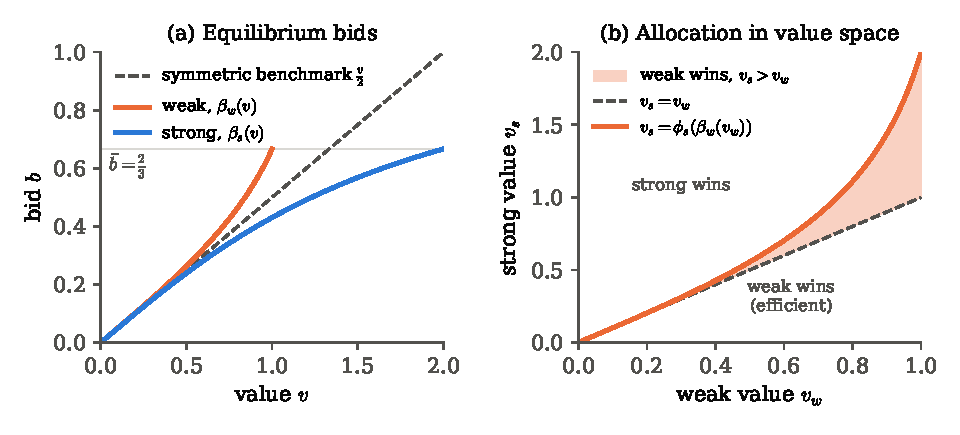
\includegraphics[width=\textwidth]{figures/ch14/asym_bids.pdf}
\caption{Asymmetric first-price auction with $V_w\sim U[0,1]$ and $V_s\sim U[0,2]$. Panel (a): the
equilibrium bid functions \eqref{eq:14-unif-beta} and the symmetric benchmark $\frac{v}{2}$. Both
bidders' bids end at the common top bid $\bar b=\frac{2}{3}$. Panel (b): the weak bidder wins below
the curve $v_s=\phi_s(\beta_w(v_w))$. In the shaded band between that curve and the diagonal the weak
bidder wins although the strong bidder values the object more.}
\label{fig:14-asym-bids}
\end{figure}

The example shows every effect of \cref{prop:14-maskin-riley}. The strong bidder's payoff falls by
$0.0764$ when we move from the second-price to the first-price auction. The weak bidder's payoff
rises by $0.0136$, and total surplus falls by $0.0205$. Revenue is total surplus minus payoffs, so
revenue rises by $0.0764-0.0136-0.0205=0.0423$. The first-price auction extracts more from the strong
bidder than it gives away to the weak bidder and to inefficiency.

\subsection{Revenue comparisons with asymmetric bidders}\label{sec:14-asym-revenue}

The decomposition used in the example holds in general:
\begin{equation}\label{eq:14-rev-decomp}
\text{expected revenue}=\text{expected total surplus}-\sum_i\E\bigl[\pi_i(V_i)\bigr].
\end{equation}
Moving from the open auction to the first-price auction lowers total surplus, by
\cref{prop:14-maskin-riley}(iii). It raises the weak bidder's rents and lowers the strong bidder's
rents, by part (iv). The net effect on revenue has no general sign.
\citet{MaskinRiley2000} give sufficient conditions on the value distributions under which the
first-price auction yields higher revenue, and others under which the open auction does. In the
uniform example the first-price auction raises more revenue. \citet[Section II.D]{AtheyLevinSeira2011} stress that ``there is no general theoretical
comparison of expected revenue, even with fixed participation.''

The optimal auction of \cref{sec:14-optimal} explains why the first-price auction often does well.
In the same example, \cref{sec:14-optimal-asym} showed that the optimal mechanism of
\citet{Myerson1981} gives the weak bidder a head start of $\frac{1}{2}$, because $\psi_w(v)=2v-1$
exceeds $\psi_s(v)=2v-2$ at every value. It earns $\frac{31}{48}\approx 0.646$, well above both
standard formats. The first-price auction tilts the allocation in the same direction as the optimal
mechanism, without design, and it captures part of the gain.
\citet[Section 7]{AtheyHaile2007} summarize the trade-off. First-price auctions may allocate
inefficiently with asymmetric bidders, but they ``tend to raise more revenue in private values
settings.''

\section{Participation and Entry}\label{sec:14-entry}

So far the set of bidders has been fixed. In practice, bidding is costly. A timber bidder must cruise
the tract to estimate its volume and quality, and a construction firm must prepare a detailed cost
estimate. Firms decide whether to incur these costs before the auction. The number of bidders is then
an equilibrium outcome, and the auction format can affect it.

Two timing assumptions organize the theory. In the first, a bidder knows its value before deciding
whether to pay the entry cost. In the second, a bidder learns its value only after paying the cost.
\citet{Samuelson1985} studies the first timing, and \citet{LevinSmith1994} study the second. The
second timing underlies the empirical work of \citet{AtheyLevinSeira2011}, where the entry cost is
the cost of cruising the tract. The two timings give the entry cost different meanings
\citep[Section~2.2, p.~91]{HortacsuPerrigne2021}. When bidders know their values, entry is
\emph{selective}, since only bidders with high enough values enter, and $K$ is a cost of preparing a
bid. When bidders learn their values after entry, entry is \emph{nonselective}, and $K$ also covers
the cost of acquiring information. \citet{RobertsSweeting2016} nest both cases. In their model each
potential bidder observes a noisy signal of its value before it decides whether to enter. The model
of \citet{LevinSmith1994} is the case of signals independent of values, and the model of
\citet{Samuelson1985} is the case of perfect correlation \citep[footnote~9, p.~92]{HortacsuPerrigne2021}.
Throughout this section, $K>0$ is the entry cost, $N$ is the number
of potential bidders, and $p$ denotes an entry probability. Elsewhere $p$ is the clock price
(\cref{sec:14-formats}) or a probability of winning (\cref{sec:14-ret-selfselection}).

\subsection{Entry with values known in advance}\label{sec:14-entry-samuelson}

Suppose each of $N$ symmetric potential bidders knows its value $v_i$, drawn independently from $F$
on $[\underline v,\bar v]$. A bidder who pays $K$ may bid in a standard auction with reserve price
$r$. We look for a symmetric equilibrium in which a bidder enters if and only if its value is at least
a cutoff $v^*$.

The cutoff type is pinned down by a simple observation. A bidder with value $v^*$ wins only if no
rival enters, because any entrant has a value above $v^*$. That happens with probability
$F(v^*)^{N-1}$, and then the lone bidder pays the reserve price. In the second-price auction this is
immediate. In the first-price auction the cutoff type also bids $r$, because it wins only when it is
alone and any higher bid would only raise its payment. Indifference of the cutoff type requires
\begin{equation}\label{eq:14-samuelson-cutoff}
(v^*-r)\,F(v^*)^{N-1}=K .
\end{equation}
Let $\Phi(v)=(v-r)F(v)^{N-1}$. It is zero at $v=r$ and strictly increasing, with
$\Phi'(v)=F(v)^{N-1}+(v-r)(N-1)F(v)^{N-2}f(v)>0$. So a unique interior cutoff exists whenever $\bar
v-r>K$. Types above $v^*$ strictly prefer to enter, because a bidder's expected surplus rises with its
value at the rate of its win probability.

Implicit differentiation of \eqref{eq:14-samuelson-cutoff} gives the comparative statics:
\[
\frac{dv^*}{dK}=\frac{1}{\Phi'(v^*)}>0,\qquad
\frac{dv^*}{dr}=\frac{F(v^*)^{N-1}}{\Phi'(v^*)}\in(0,1),\qquad
\frac{dv^*}{dN}=-\frac{(v^*-r)F(v^*)^{N-1}\ln F(v^*)}{\Phi'(v^*)}>0,
\]
where the last expression treats $N$ as continuous. The entry cost and the reserve price both screen
out low-value bidders. A higher reserve raises the cutoff by less than one for one. The entry cost
differs from a reserve price in one respect. It is a resource cost borne by every entrant, and the
seller collects none of it.

\begin{example}[Cutoffs with uniform values]\label{ex:14-samuelson}
Let $F$ be uniform on $[0,1]$, $N=5$ and $r=0$. Equation \eqref{eq:14-samuelson-cutoff} becomes
$(v^*)^5=K$, so $v^*=K^{\frac{1}{5}}$. With $K=0.05$ the cutoff is $0.549$, each potential bidder
enters with probability $0.451$, and $2.25$ bidders enter on average. With $K=0.10$ the cutoff is
$0.631$ and $1.85$ bidders enter on average. Raising the reserve to $r=0.25$ raises the cutoffs to
$0.610$ and $0.690$. These values come from \texttt{entry\_example.py}.
\end{example}

With values known in advance, the entrants are a selected sample of high-value bidders. This
complicates both theory and estimation. \citet[Section II.F]{AtheyLevinSeira2011} note that with
asymmetric bidders who have prior private information, ``the ex ante rankings of strong and weak
bidders may fail to hold conditional on entry.'' This is one reason they adopt the second timing.

\subsection{Entry with values learned after entry: the Levin-Smith model}\label{sec:14-entry-ls}

Now suppose a bidder learns its value only after paying $K$. Before entry, all $N$ potential bidders
are identical. Entrants observe the number of other entrants before bidding
\citep[Section 6.3.2]{AtheyHaile2007}. Let $\pi(k)$ be the expected profit, gross of $K$, of an
entrant when $k$ bidders enter in total, so that it faces $k-1$ rivals. We study the symmetric
equilibrium in which each potential bidder enters with probability $p$.

Given that the other $N-1$ potential bidders each enter with probability $p$, the number of rival
entrants is binomial. An entrant's ex ante expected profit is therefore
\begin{equation}\label{eq:14-entry-indiff}
\Pi(p)=\sum_{k=1}^{N}\binom{N-1}{k-1}p^{k-1}(1-p)^{N-k}\,\pi(k).
\end{equation}
A potential bidder enters with probability one if $\Pi(p)>K$, stays out if $\Pi(p)<K$, and is willing
to randomize if $\Pi(p)=K$.

\begin{lemma}\label{lem:14-pi-decreasing}
In the symmetric private values model with any standard auction and reserve price $r$, the gross
profit of an entrant is
\begin{equation}\label{eq:14-pik}
\pi(k)=\int_r^{\bar v}F(t)^{k-1}\bigl(1-F(t)\bigr)dt ,
\end{equation}
which is strictly decreasing in $k$. With values uniform on $[0,1]$ and $r=0$,
$\pi(k)=\frac{1}{k(k+1)}$.
\end{lemma}

\begin{proof}
By revenue equivalence, an entrant's interim surplus is the same in every standard auction. By
\cref{lem:14-ic}, a type $v\ge r$ facing $k-1$ rivals earns $\int_r^vF(t)^{k-1}dt$, and types below
$r$ earn zero. Taking expectations and exchanging the order of integration,
\[
\pi(k)=\int_r^{\bar v}\left[\int_r^{v}F(t)^{k-1}dt\right]f(v)\,dv
=\int_r^{\bar v}F(t)^{k-1}\left[\int_t^{\bar v}f(v)\,dv\right]dt
=\int_r^{\bar v}F(t)^{k-1}\bigl(1-F(t)\bigr)dt .
\]
Since $F(t)<1$ on the interior of the support, the integrand falls strictly in $k$. In the uniform
case, $\pi(k)=\int_0^1t^{k-1}(1-t)\,dt=\frac{1}{k}-\frac{1}{k+1}=\frac{1}{k(k+1)}$.
\end{proof}

\begin{proposition}[Symmetric entry equilibrium]\label{prop:14-ls-unique}
Suppose $\pi(k)$ is strictly decreasing in $k$ and $N\ge 2$. Then $\Pi(p)$ is strictly decreasing in
$p$, and there is a unique symmetric entry equilibrium $p^*$. If $\pi(N)\ge K$, then $p^*=1$. If
$\pi(1)\le K$, then $p^*=0$. Otherwise $p^*\in(0,1)$ solves $\Pi(p^*)=K$.
\end{proposition}

\begin{proof}
Let $X\sim\text{Binomial}(N-1,p)$ be the number of rival entrants, so $\Pi(p)=\E[\pi(1+X)]$. A
binomial random variable is stochastically increasing in its success probability. Since $\pi$ is
strictly decreasing, $\E[\pi(1+X)]$ is strictly decreasing in $p$. The function is continuous, with
$\Pi(0)=\pi(1)$ and $\Pi(1)=\pi(N)$. The three cases follow from the intermediate value theorem and
strict monotonicity.
\end{proof}

When $p^*\in(0,1)$, entrants earn zero expected profit net of the entry cost. This has a striking
consequence. Let the seller value the object at $v_0$, and let $S(k)$ be the expected gain from trade
when $k$ bidders enter, measured relative to the seller keeping the object. It equals the expected
value of the winner minus $v_0$ when a sale occurs, and zero otherwise. The seller's expected gain,
revenue minus $v_0$ times the probability of sale, equals expected gains from trade minus bidders'
expected gross rents. Gross rents sum to $Np^*\Pi(p^*)=Np^*K$. Hence
\begin{equation}\label{eq:14-ls-revenue}
\text{seller's expected gain}=\E\bigl[S(X^*)\bigr]-Np^*K,\qquad X^*\sim\text{Binomial}(N,p^*).
\end{equation}
The right side is expected social welfare. The seller captures all of the social surplus, net of
entry costs. With $v_0=0$ the seller's gain is its expected revenue.

\begin{proposition}[Levin and Smith 1994]\label{prop:14-ls-welfare}
Consider symmetric private values, a seller who values the object at $v_0$, and an efficient standard
auction with reserve price $r=v_0$. Then:
\begin{enumerate}[label=(\roman*)]
\item Social welfare $W(p)=\E[S(X)]-NpK$, with $X\sim\text{Binomial}(N,p)$, satisfies
$W'(p)=N\bigl(\Pi(p)-K\bigr)$. The equilibrium entry probability maximizes welfare among symmetric
entry probabilities.
\item If $p^*\in(0,1)$ at $r=v_0$, no reserve price gives the seller a higher expected gain than
$r=v_0$.
\end{enumerate}
\end{proposition}

\begin{proof}
(i) Write $X=\sum_{j=1}^{N}\epsilon_j$ with independent entry indicators $\epsilon_j$ that equal one
with probability $p_j$. Differentiating $\E[S(X)]$ with respect to $p_j$ gives
$\E[S(Y_{-j}+1)-S(Y_{-j})]$, where $Y_{-j}$ counts the other entrants. At $p_j=p$ for all $j$,
summing over $j$ yields
\[
\frac{d}{dp}\E[S(X)]=N\,\E\bigl[S(Y+1)-S(Y)\bigr],\qquad Y\sim\text{Binomial}(N-1,p).
\]
With $r=v_0$ and an efficient auction, $S(k)=\E\bigl[(\max\{V_1,\dots,V_k\}-v_0)^+\bigr]$. The
increment $S(k+1)-S(k)$ is then the expected marginal contribution of one more bidder,
$\E\bigl[(V_{k+1}-\max\{V_1,\dots,V_k,v_0\})^+\bigr]$. In a second-price auction with reserve $v_0$,
this is exactly the bidder's expected surplus when it faces $k$ rivals, which is $\pi(k+1)$. By
revenue equivalence the same holds in any efficient standard auction with reserve $v_0$. Therefore
$\frac{d}{dp}\E[S(X)]=N\,\E[\pi(Y+1)]=N\,\Pi(p)$, and $W'(p)=N(\Pi(p)-K)$. Since $\Pi$ is decreasing,
$W$ is concave, and its maximizer over $[0,1]$ is the $p^*$ of \cref{prop:14-ls-unique}.

(ii) Let $R(r)$ and $W_r(p)$ denote the seller's expected gain and welfare with reserve $r$, and let
$p^*(r)$ be the equilibrium entry probability. Net bidder rents are never negative in equilibrium, so $R(r)\le
W_r(p^*(r))$. For any fixed $p$, the reserve $v_0$ allocates the object efficiently among the
entrants and the seller, so $W_r(p)\le W_{v_0}(p)$. By part (i), $W_{v_0}(p)\le W_{v_0}(p^*(v_0))$.
Finally, \eqref{eq:14-ls-revenue} gives $W_{v_0}(p^*(v_0))=R(v_0)$ when $p^*(v_0)\in(0,1)$. Chaining
the inequalities, $R(r)\le R(v_0)$.
\end{proof}

Part (ii) reverses the logic of \cref{cor:14-optimal-reserve}. With a fixed number of bidders, the
seller sets a reserve above its own value to extract rents. With endogenous entry and zero expected
rents, there are no rents left to extract. A reserve above $v_0$ then only discourages entry and
distorts the allocation. \citet[Section~2.2, p.~91]{HortacsuPerrigne2021} state the contrast between
the two entry models. Under nonselective entry of the Levin-Smith type, the optimal reserve price is
the seller's own value. Under selective entry it is given by the formula \eqref{eq:14-optimal-reserve}
of the fixed-participation model. The proofs here are our own.
\citet{LevinSmith1994} also show that the random entry of the mixed
equilibrium wastes resources. Sometimes too many bidders enter and sometimes too few. A seller who
could limit the number of potential bidders, and charge an entry fee if needed, would earn more.

\begin{example}[Levin-Smith entry with uniform values]\label{ex:14-ls}
Let values be uniform on $[0,1]$, $r=v_0=0$ and $N=5$. By \cref{lem:14-pi-decreasing},
$\pi(1),\dots,\pi(5)=\frac{1}{2},\frac{1}{6},\frac{1}{12},\frac{1}{20},\frac{1}{30}$, so
$\Pi(1)=\pi(5)=\frac{1}{30}\approx 0.033$. Every entry cost between $\frac{1}{30}$ and $\pi(1)=\frac{1}{2}$ therefore
produces a mixed equilibrium. For $K\ge\frac{1}{2}$ nobody enters. With $K=0.05$, solving $\Pi(p)=K$ numerically gives $p^*=0.816$, so $4.08$
bidders enter on average. Expected revenue equals expected welfare, $0.592$. With $K=0.10$, $p^*=0.559$,
$2.79$ bidders enter on average, nobody enters with probability $0.017$, and revenue is $0.425$.
\Cref{fig:14-entry}(a) shows the two solutions.

The value of limiting entry is visible in \cref{fig:14-entry}(b). With $K=0.05$ and $N=4$ potential
bidders, $\pi(4)=\frac{1}{20}=K$, so all four enter and revenue is $\frac{3}{5}=0.600$. Adding a fifth
potential bidder lowers revenue to $0.592$, and ten potential bidders lower it to $0.574$. With
$K=0.10$, revenue peaks at $0.452$ with $N=3$. The losses are modest here, but they have the sign
that \citet{LevinSmith1994} emphasize. All numbers come from \texttt{entry\_example.py}.
\end{example}

\begin{figure}[htbp]
\centering
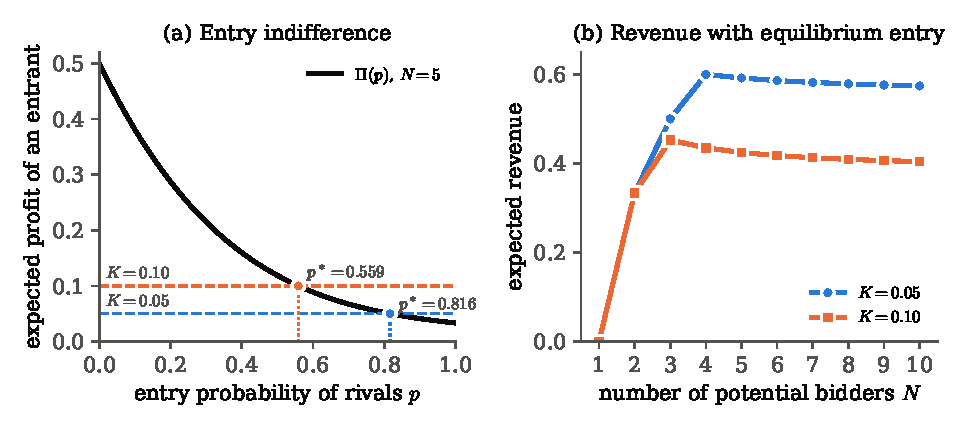
\includegraphics[width=\textwidth]{figures/ch14/entry.pdf}
\caption{Levin-Smith entry with uniform values and no reserve price. Panel (a): the ex ante profit of
an entrant $\Pi(p)$ in \eqref{eq:14-entry-indiff} for $N=5$, and the equilibrium entry probabilities
for $K=0.05$ and $K=0.10$. Panel (b): expected revenue in the symmetric entry equilibrium as a
function of the number of potential bidders $N$.}
\label{fig:14-entry}
\end{figure}

\subsection{Asymmetric bidders and type-symmetric entry equilibria}\label{sec:14-entry-als}

\citet{AtheyLevinSeira2011} combine the Levin-Smith timing with the asymmetric model of
\cref{sec:14-asym}. There are $N_L$ potential loggers with value distribution $F_L$ and $N_M$
potential mills with value distribution $F_M$. Mills are strong: $F_M$ dominates $F_L$ in the
reverse hazard rate order. Each firm decides independently whether to pay $K$, learns its value if it
does, and learns which rivals entered before bidding \citep[Section II.A]{AtheyLevinSeira2011}.

The model omits two features that could also matter for the format comparison. Bidders may have a
common value component, from private estimates of timber quality and volume or from differing
beliefs about future market conditions. They may also be risk averse. \citet[Section
II.F]{AtheyLevinSeira2011} abstract from both for two reasons. The format differences they observe
are qualitatively different from those that common values or risk aversion would imply, and
including either feature significantly complicates the analysis. They also restrict attention to
type-symmetric equilibria, which they regard as a convenient assumption that allows point
identification of entry costs.

Let $\pi_L^\tau(n_L,n_M)$ and $\pi_M^\tau(n_L,n_M)$ be the expected profits, gross of $K$, of a
participating logger and mill in format $\tau\in\{\mathrm{o},\mathrm{s}\}$ (open or sealed). The superscript $\tau$ indexes the format
and is unrelated to the payment rule $\tau_i$ of \cref{sec:14-ret}. The
participants are $n_L$ loggers and $n_M$ mills, and these counts include the bidder itself. Following
\citet[eq.~(4)]{AtheyLevinSeira2011}, bidder $i$'s ex ante profit from entering is
\begin{equation}\label{eq:14-als-exante}
\Pi_i^\tau(\bm p)=\sum_{\bm n}\pi_i^\tau(n_L,n_M)\,\Pr\bigl[n_L,n_M\mid i\text{ enters, rivals play }\bm p_{-i}\bigr],
\end{equation}
where $\bm p$ is the profile of entry probabilities. When all loggers enter with probability $p_L$ and
all mills with probability $p_M$, the probabilities are binomial. Write
$\mathrm{bin}(k;m,p)=\binom{m}{k}p^k(1-p)^{m-k}$. For a logger and a mill, respectively,
\begin{align}
\Pi_L^\tau(p_L,p_M)&=\sum_{n_L=1}^{N_L}\sum_{n_M=0}^{N_M}\mathrm{bin}(n_L-1;N_L-1,p_L)\,\mathrm{bin}(n_M;N_M,p_M)\,\pi_L^\tau(n_L,n_M),\label{eq:14-als-PiL}\\
\Pi_M^\tau(p_L,p_M)&=\sum_{n_L=0}^{N_L}\sum_{n_M=1}^{N_M}\mathrm{bin}(n_L;N_L,p_L)\,\mathrm{bin}(n_M-1;N_M-1,p_M)\,\pi_M^\tau(n_L,n_M).\label{eq:14-als-PiM}
\end{align}

\begin{definition}[Type-symmetric entry equilibrium]\label{def:14-type-symmetric}
A \emph{type-symmetric entry equilibrium} \citep[Section II.A]{AtheyLevinSeira2011} consists of bid
strategies $b_L(\cdot;\bm n)$, $b_M(\cdot;\bm n)$ and entry probabilities $p_L$, $p_M$ with three
properties.
\begin{enumerate}[label=(\roman*)]
\item All loggers use $(b_L,p_L)$ and all mills use $(b_M,p_M)$.
\item Each bidder's bid strategy maximizes its profit conditional on entering, for every set of
participants.
\item Each bidder enters if and only if its expected profit from entry \eqref{eq:14-als-exante} is at
least $K$. It may randomize when the two are equal.
\end{enumerate}
\end{definition}

Bid strategies in the open auction are $b_k(v;\bm n)=v$. In the sealed auction they solve
\eqref{eq:14-ts-foc-L} and \eqref{eq:14-ts-foc-M} with $b_k(r;\bm n)=r$. A type-symmetric entry
equilibrium exists in both formats, but it need not be unique \citep[Section
II.C]{AtheyLevinSeira2011}. The following condition, with at least two potential bidders of each
type, restores uniqueness. For the proof we maintain
that a participant's expected profit falls when a rival is added, strictly in expectation. In the
open auction this holds auction by auction, since a bidder's surplus
$(v-\max\{\text{rival values},r\})^+$ can only fall when a rival is added.

\begin{proposition}[Athey, Levin and Seira 2011, Proposition 1]\label{prop:14-als-unique}
Suppose that for all $n_L,n_M$,
\begin{equation}\label{eq:14-als-condition}
\pi_M^{\mathrm{s}}(n_L,n_M+1)>\pi_L^{\mathrm{s}}(n_L,n_M).
\end{equation}
Then every type-symmetric entry equilibrium of either auction format has $p_L=0$ or $p_M=1$. If
also $N_L\ge 2$ and $N_M\ge 2$, each format has a unique type-symmetric entry equilibrium.
\end{proposition}

Condition \eqref{eq:14-als-condition} compares a mill and a logger that face the same $n_M$ mills.
The mill faces $n_L$ loggers, while the logger faces only $n_L-1$ other loggers. The condition
requires the mill to earn more despite its extra rival. In the words of \citet[Section
II.C]{AtheyLevinSeira2011}, ``mills have a sufficient value advantage over loggers to outweigh the
effects of facing an additional bidder.'' They call the condition ``rather strong'' as theory, and
they verify it for every tract in their estimated model (\cref{ch:auction-empirics}).

\begin{proof}[Proof sketch]
\emph{Mills earn more than loggers at every entry profile.} Fix $(p_L,p_M)$. A logger who enters
faces $X_L\sim\text{Binomial}(N_L-1,p_L)$ other loggers and $X_M\sim\text{Binomial}(N_M,p_M)$ mills. A
mill who enters faces $X_L+\epsilon_L$ loggers and $X_M-\epsilon_M$ other mills. Here $\epsilon_L$ is an
indicator with success probability $p_L$, independent of everything else, and $\epsilon_M$ is the entry
indicator of one of the $N_M$ mills counted in $X_M$. Then $X_L+\epsilon_L\sim\text{Binomial}(N_L,p_L)$
and $X_M-\epsilon_M\sim\text{Binomial}(N_M-1,p_M)$, as a mill's counts require. Using monotonicity, then \eqref{eq:14-als-condition}, then monotonicity again,
\[
\pi_M(X_L+\epsilon_L,\,X_M-\epsilon_M+1)\ \ge\ \pi_M(X_L+1,\,X_M-\epsilon_M+1)\ >\
\pi_L(X_L+1,\,X_M-\epsilon_M)\ \ge\ \pi_L(X_L+1,\,X_M).
\]
Taking expectations gives $\Pi_M(p_L,p_M)>\Pi_L(p_L,p_M)$ for every profile.

\emph{Either $p_L=0$ or $p_M=1$.} If loggers enter with positive probability, then $\Pi_L\ge K$. The
previous step gives $\Pi_M>K$, so mills enter with probability one.

\emph{Uniqueness.} Candidate equilibria have either $p_M=1$ and $p_L$ solving the logger's condition,
or $p_L=0$ and $p_M<1$ solving the mill's condition. With all mills entering, a logger's payoff is
$\Pi_L(p_L,1)=\E[\pi_L(1+X_L,N_M)]$. When $N_L\ge 2$, the count $X_L$ of other loggers is
stochastically increasing in $p_L$, so $\Pi_L(\cdot,1)$ is strictly decreasing. When $N_M\ge 2$, the
same argument shows that $\Pi_M(0,\cdot)$ is strictly decreasing. Each family therefore has at most
one member. Suppose an equilibrium with $p_L=0$
and $p_M<1$ exists. Then $\Pi_M(0,p_M)\le K$ when $p_M=0$, or $\Pi_M(0,p_M)=K$ when $p_M>0$. In
either case $\Pi_M(p_L,1)\le\Pi_M(0,1)<\Pi_M(0,p_M)\le K$ for every $p_L$, so no equilibrium with
$p_M=1$ exists. Only one candidate survives.

\emph{Both formats.} For any participant set, mills earn more and loggers less in the open auction
than in the sealed auction \citep[Section II.D]{AtheyLevinSeira2011}. This is the many-bidder
analogue of \cref{prop:14-maskin-riley}(iv). Hence
$\pi_M^{\mathrm{o}}(n_L,n_M+1)\ge\pi_M^{\mathrm{s}}(n_L,n_M+1)>\pi_L^{\mathrm{s}}(n_L,n_M)\ge\pi_L^{\mathrm{o}}(n_L,n_M)$,
and the argument applies to the open auction as well.
\end{proof}

\citet{AtheyLevinSeira2011} state uniqueness without the restriction $N_L,N_M\ge 2$, and the
restriction matters. With a single potential logger, $\Pi_L(p_L,1)=\pi_L(1,N_M)$ does not depend on
$p_L$. If $K=\pi_L(1,N_M)$, the logger is indifferent at every $p_L$, and mills strictly prefer to
enter by the first step of the proof. Every profile $(p_L,1)$ with $p_L\in[0,1]$ is then an
equilibrium. With one mill and one logger in the sealed auction of \cref{ex:14-als-entry} below, this
happens at $K=\pi_L^{\mathrm{s}}(1,1)=0.0969$. A single potential mill creates the same indifference at
$K=\pi_M(0,1)$, the profit of a mill without rivals, where every profile $(0,p_M)$ is an equilibrium.
At every other entry cost, a payoff that does not depend on its own type's entry probability is either
above or below $K$. It then pins down a single entry probability, and the equilibrium is again unique.
The separation result, $p_L=0$ or $p_M=1$, holds for any numbers of potential bidders.

The empirically relevant equilibrium has every mill entering and loggers randomizing,
$p_M=1$ and $p_L\in(0,1)$. \citet[Section II.C]{AtheyLevinSeira2011} motivate this case with their
data: they ``observe logger entry in more than 85\% of sales and always more potential logger
entrants than actual logger entrants.''

\casehead{The homogeneous benchmark}
If $F_L=F_M$, every bidder is the same and revenue equivalence applies conditional on the number of
entrants. Each format then produces the same $\pi(k)$, given by \eqref{eq:14-pik}, and the same
entry condition. \citet[Section II.D]{AtheyLevinSeira2011} conclude that the two formats have
``(i) the same expected entry, (ii) the same allocation, and (iii) the same expected revenue.''
Format differences in entry therefore require asymmetric bidders.

\begin{proposition}[Athey, Levin and Seira 2011, Proposition 2]\label{prop:14-entry-format}
For any type-symmetric entry equilibrium of the sealed bid auction, there is a type-symmetric entry
equilibrium of the open auction with the following properties.
\begin{enumerate}[label=(\roman*)]
\item Loggers are less likely to enter.
\item Mills are more likely to enter.
\item It is less likely that a logger wins.
\end{enumerate}
\end{proposition}

\begin{proof}[Proof sketch for the empirically relevant case]
Assume \eqref{eq:14-als-condition} and $N_L,N_M\ge 2$, so each format has a unique equilibrium by
\cref{prop:14-als-unique}, and suppose the sealed
equilibrium has $p_M^{\mathrm{s}}=1$ and $p_L^{\mathrm{s}}\in(0,1)$. For every participant set, a
logger earns weakly less in the open auction. Hence $\Pi_L^{\mathrm{o}}(p_L,1)\le\Pi_L^{\mathrm{s}}(p_L,1)$
for every $p_L$. At $p_L^{\mathrm{s}}$ the sealed condition holds with equality, so
$\Pi_L^{\mathrm{o}}(p_L^{\mathrm{s}},1)\le K$. Because $\Pi_L^{\mathrm{o}}(\cdot,1)$ is decreasing,
the open-auction solution satisfies $p_L^{\mathrm{o}}\le p_L^{\mathrm{s}}$. This is (i). Mills earn
weakly more in the open auction and face fewer loggers, so
$\Pi_M^{\mathrm{o}}(p_L^{\mathrm{o}},1)\ge\Pi_M^{\mathrm{s}}(p_L^{\mathrm{s}},1)\ge K$. Mills still enter
with probability one, which gives (ii) with equality. For (iii), two effects reinforce each other.
For a fixed set of participants, a logger wins less often in the open auction, which is efficient,
than in the sealed auction, by \cref{prop:14-maskin-riley}(iii). In the open auction, fewer logger
entrants also mean a lower chance that the highest value belongs to a logger.
\end{proof}

The general statement allows multiple equilibria, which is why it is phrased as existence of a
suitable open-auction equilibrium. Under the conditions of \cref{prop:14-als-unique}, the prediction
is sharp: ``open
bidding leads to less logger entry, equivalent mill entry and a lower chance that a logger wins''
\citep[Section II.D]{AtheyLevinSeira2011}. The revenue comparison remains ambiguous. Sealed bidding
attracts more loggers, which raises competition, but it allocates inefficiently. The sealed auction is
``inefficient even conditional on participation,'' while the efficient type-symmetric outcome is an
equilibrium of the open auction \citep[Section II.D, citing \citealp{AtheyLevinSeira2004}]{AtheyLevinSeira2011}. The idea that sealed bids
encourage entry by weaker bidders is emphasized by \citet{Klemperer2004} in the context of spectrum
auctions \citep[footnote~4, p.~215]{AtheyLevinSeira2011}. \citet[Section~7]{AtheyHaile2007} likewise
list entry among the factors that govern the choice of format. The format ``also affects bidder entry
when bidders are asymmetric,'' and they cite \citet{Klemperer2002} and \citet{AtheyLevinSeira2004}. The
mechanism is the one of \cref{prop:14-entry-format}. An ascending auction deters entry by bidders who
expect to be outbid by a stronger rival.
\citet{Klemperer2002} proposes hybrid formats that end with a sealed-bid stage.

\begin{example}[One mill and one potential logger]\label{ex:14-als-entry}
Take the values of \cref{ex:14-asym-uniform}: the mill draws from $U[0,2]$, the logger from
$U[0,1]$, and $r=0$. With both present, \cref{tab:14-asym-example} gives
$\pi_L^{\mathrm{s}}=0.0969$, $\pi_L^{\mathrm{o}}=\frac{1}{12}\approx 0.0833$,
$\pi_M^{\mathrm{s}}=0.5069$ and $\pi_M^{\mathrm{o}}=\frac{7}{12}$. A mill alone pays the reserve and
earns $\E[V_M]=1$, and a logger alone earns $\E[V_L]=\frac{1}{2}$. Condition
\eqref{eq:14-als-condition} holds, since $0.5069>0.5$. Let $K=0.09$. This cost differs from the
knife-edge values $\pi_L^\tau(1,1)$ and $\pi_M^\tau(0,1)=1$ of both formats, so each format has a
unique type-symmetric entry equilibrium. In the sealed auction the mill
enters and the logger enters too, because $0.0969>0.09$. Revenue is $0.459$, the logger wins with
probability $\frac{1}{3}$, and welfare is $1.0628-2K=0.883$. In the open auction the logger stays
out, because $0.0833<0.09$. The mill wins at the reserve price, so revenue is zero and welfare is
$1-K=0.91$. The sealed auction raises far more revenue through entry, and the open auction is more
efficient.
\end{example}

The example is extreme because $r=0$, but it isolates the mechanism of \cref{prop:14-entry-format}.
The weak bidder's expected profit is higher under sealed bidding, so it enters more often. That entry
disciplines the strong bidder, whose price would otherwise be set by the reserve.

\casehead{From entry decisions to entry costs}
The indifference of randomizing bidders carries empirical content. For any bidder who randomizes,
expected profit from entry equals $K$. \citet[Section 6.3.2]{AtheyHaile2007} write this as
\begin{equation}\label{eq:14-entry-cost-id}
K=\sum_{\mathcal A:\,i\in\mathcal A}\Pr\bigl(\tilde{\mathcal N}=\mathcal A\mid i\in\tilde{\mathcal
N}\bigr)\,\pi_i(\mathcal A),
\end{equation}
where $\tilde{\mathcal N}$ is the random set of entrants. Here $\pi_i(\mathcal A)$ is bidder $i$'s
expected gross profit when the participant set is $\mathcal A$,
\begin{equation}\label{eq:14-entry-profit-id}
\pi_i(\mathcal A)=\E\Bigl[\bigl(V_i-\beta_i(V_i;\mathcal A)\bigr)\,G_{M_i|B_i}\bigl(\beta_i(V_i;\mathcal
A)\bigm|\beta_i(V_i;\mathcal A);\mathcal A\bigr)\Bigr],
\end{equation}
with $G_{M_i|B_i}$ the distribution of the highest rival bid given bidder $i$'s own bid. The notation
follows \citet[Section 6.3.2]{AtheyHaile2007}, who write $\Pi_i$ for what we call $\pi_i$. The post-entry profits are identified
from bids, and the entry probabilities are observed. The level of the entry cost is then identified
in dollars. This contrasts with entry models that infer profits only from entry decisions
\citep[Section 6.3.2]{AtheyHaile2007}. \Cref{ch:auction-empirics} develops the estimator.

\section{Collusion and the Choice of Format}\label{sec:14-collusion}

Collusion among bidders is a long-standing concern in auction design. Gifford Pinchot, the first
chief of the US Forest Service, advocated sealed bidding for timber. He described a sale on sealed
bids as ``thereby preventing the customary collusion between bidders'' \citep[p.~209]{Pinchot1998},
as quoted by \citet[footnote 2]{AtheyLevinSeira2011}. \citet[Section 9]{MilgromWeber1982} name the
same setting as a limit of their noncooperative theory. They judge it less reasonable for timber
rights on federal land, where ``the bidders (owners of lumber mills) are members of a trade
association and bid repeatedly against each other'' \citep[p.~1118]{MilgromWeber1982}. This section explains why the format matters for collusion. The
general theory of cartels is in \cref{ch:collusion-theory}, and prosecuted bidding rings are studied
in \cref{ch:collusion-evidence}.

\subsection{Rings in second-price and ascending auctions}\label{sec:14-collusion-open}

A \emph{bidding ring} is a group of bidders who agree to suppress competition among themselves.
Consider the private values model with a ring $\mathcal C\subset\mathcal N$ of $m\ge 2$ members.
Suppose for now that members know each other's values. The simplest agreement designates the member
with the highest value, bidder $d$, to bid. The other members abstain or bid the reserve price.
Bidders outside the ring bid as usual.

\begin{proposition}[Robinson 1985]\label{prop:14-robinson}
In a second-price or ascending auction with private values, the ring agreement in which the
highest-value member bids its value and the other members abstain is self-enforcing. No member gains
by deviating within the auction, whatever the values and whether or not the members meet again.
\end{proposition}

\begin{proof}
Outsiders bid their values, which is weakly dominant by \cref{prop:14-spa-dominant}. The designated
bidder $d$ bids $v_d$, which is also weakly dominant. Consider a member $j\neq d$, with $v_j\le v_d$.
Bidder $j$ wins only with a bid above $v_d$, since $d$ stays in until the price reaches $v_d$. A
winning deviation then pays at least $v_d\ge v_j$, so its payoff is at most zero. Abstaining yields
zero. Hence no deviation is profitable.
\end{proof}

The ring gains because it removes the price pressure that members exert on each other. Let
$V^{\mathcal C}_{(1)}\ge V^{\mathcal C}_{(2)}$ be the two highest member values and $V^{\mathcal O}_{(1)}$
the highest outsider value. Competitive bidding sets the price at the second-highest value overall.
Under the ring, the price is $\max\{V^{\mathcal O}_{(1)},r\}$ whenever a member wins. The price
falls only when the two highest values both belong to members, and then by
\begin{equation}\label{eq:14-ring-gain}
\Delta P=\Bigl(V^{\mathcal C}_{(2)}-\max\bigl\{V^{\mathcal O}_{(1)},r\bigr\}\Bigr)^+ .
\end{equation}
The ring does not change who wins, so the allocation stays efficient. The ring transfers surplus
from the seller to its members.

\Citet[Section~2.5, p.~96]{HortacsuPerrigne2021} draw the practical lesson from \cref{prop:14-robinson}.
Open auctions may favor collusion, because bidders meet face to face and can react at once to each
other's behavior. If the ring allocates the object to its highest-value member, no other member gains
by deviating, since that member can always outbid the deviator. For this reason auction theorists
recommend first-price auctions. The issue is practical. Collusion at U.S.\ Forest Service timber sales
was suspected in the 1970s, and it was the subject of allegations and of a congressional hearing in
1977, though few cases were prosecuted. In 1976 the federal government recommended first-price sealed
bids over ascending auctions, mainly to reduce collusion \citep[Section~2.4, p.~96]{HortacsuPerrigne2021}.
Sealed bids are no cure, however. The same survey reviews collusion in first-price procurement auctions
of construction contracts (their Section~3.4), and \cref{ch:collusion-evidence} studies such rings.

\subsection{Rings in first-price auctions}\label{sec:14-collusion-fpa}

The first-price auction is different. To gain, the designated bidder must bid less than the price
that competition would produce. Every other member with a value above that bid then has a unilateral
incentive to bid slightly more and win. In a one-shot auction, the designated bid must exceed the
values of all other members to deter such deviations. With known values, the ring must therefore pay
at least $V^{\mathcal C}_{(2)}$ whenever it wins. The price suppression of \eqref{eq:14-ring-gain}
cannot be sustained within a single sealed-bid auction.

Sustaining a first-price ring requires the threat of future punishment. A member who undercuts the
designated bidder is detected only after the bids are opened, and the ring can respond only in later
auctions. The agreement survives if the one-time gain from undercutting is smaller than the discounted
loss from the ring's collapse, a condition of the kind derived in \cref{ch:collusion-theory}. The
open auction needs no such condition. A deviation there is observed as it happens, and the designated
bidder answers it by continuing to bid. \citet[Section 7]{AtheyHaile2007} summarize the comparison:
first-price auctions ``may be less susceptible to collusion (detection and response to defections
are more difficult than in an ascending auction).'' This is why sealed bids appear in \cref{tab:14-ranking}
as the format less prone to collusion. \citet{Robinson1985} draws the policy conclusion that a seller
worried about rings should prefer the first-price format.

\subsection{Ring size, leakage and secret deviations}\label{sec:14-collusion-size}

The two formats also differ in who gains from a ring that does not include every bidder.
\citet[ch.~8, p.~176]{MarshallMarx2012} put the contrast as follows. In the ascending auction the
highest-value member stays in up to its value, exactly as it would without the ring. An outsider who
wins pays what it would have paid without collusion, so the ring captures all the gains. In the
sealed-bid auction the designated member bids strictly less than its noncollusive bid. Outsiders then
sometimes win auctions that they would have lost under competition. Part of the collusive gain spills
over to the outsiders, which \citet[p.~181]{MarshallMarx2012} call \emph{leakage}. The following example
computes the ascending-auction side of the comparison in closed form.

\begin{example}[Ring size with uniform values]\label{ex:14-ring-size}
Let $n$ bidders have values that are independent and uniform on $[0,1]$, with $r=v_0=0$. A ring of
$k\ge 1$ members bids in an ascending auction as in \cref{prop:14-robinson}, and the other $m=n-k$
bidders bid their values. We compute the expected price and the expected surplus of each bidder.

\emph{Step 1 (price reduction).} By \eqref{eq:14-ring-gain} with $r=0$, the ring lowers the price by
$(C_2-O_1)^+$. Here $C_2$ is the second-highest member value and $O_1$ the highest outsider value, with
$O_1=0$ when $m=0$. The density of $C_2$ is $k(k-1)x^{k-2}(1-x)$ on $[0,1]$, and $\Pr(O_1\le y)=y^m$.
For a fixed $x$,
\[
\E\bigl[(x-O_1)^+\bigr]=\int_0^x\Pr(O_1\le y)\,dy=\int_0^x y^m\,dy=\frac{x^{m+1}}{m+1}.
\]
Integrating over $C_2$ and using $k+m=n$,
\[
\E[\Delta P]=\frac{k(k-1)}{m+1}\int_0^1x^{n-1}(1-x)\,dx
=\frac{k(k-1)}{m+1}\left(\frac{1}{n}-\frac{1}{n+1}\right)
=\frac{k(k-1)}{(n-k+1)\,n\,(n+1)}.
\]

\emph{Step 2 (price).} Without a ring the expected price is $\E[V_{(n-1:n)}]=\frac{n-1}{n+1}$, so the
expected price with a ring of $k$ members is
\begin{equation}\label{eq:14-ring-price}
\E[P_k]=\frac{n-1}{n+1}-\frac{k(k-1)}{(n-k+1)\,n\,(n+1)}.
\end{equation}
With $k=2$ the fall is $\frac{2}{(n-1)n(n+1)}$.

\emph{Step 3 (surplus).} An outsider wins only with the highest value overall, and it then pays the
second-highest value overall, ring or no ring. Its expected surplus is therefore unchanged at
$\frac{1}{n}\E\bigl[V_{(n:n)}-V_{(n-1:n)}\bigr]=\frac{1}{n(n+1)}$. Members keep their competitive surplus
$\frac{k}{n(n+1)}$ and gain $\E[\Delta P]$ in addition. Per member,
\[
\frac{1}{k}\left[\frac{k}{n(n+1)}+\frac{k(k-1)}{(n-k+1)n(n+1)}\right]
=\frac{1}{n(n+1)}\cdot\frac{n}{n-k+1}
=\frac{1}{(n+1)(n-k+1)}.
\]
An all-inclusive ring, $k=n$, pays nothing, and each member earns $\frac{1}{n+1}=\frac{1}{n}\E[V_{(n:n)}]$.
\end{example}

\Cref{tab:14-mm-ring} reproduces Table~8.1 of \citet[ch.~8, p.~182]{MarshallMarx2012}, which compares
the two formats with five bidders. The ascending columns follow from \cref{ex:14-ring-size}. For
example, with $n=5$ and $k=3$, \eqref{eq:14-ring-price} gives $\frac{4}{6}-\frac{6}{3\cdot 30}=0.600$, and
each member earns $\frac{1}{6\cdot 3}\approx 0.056$. In the first-price auction the ring is a single
strong bidder whose value is the highest of $k$ uniform draws. That asymmetric auction has no closed
form. Marshall and Marx take its values from \citet[Table~III]{MarshallEtAl1994}, who compute them by
Monte Carlo with 100,000 draws.

\begin{table}[htbp]
\centering
\caption{Rings of different sizes with five bidders and uniform values}\label{tab:14-mm-ring}
\begin{tabular}{@{}ccccccc@{}}
\toprule
& \multicolumn{2}{c}{Expected price} & \multicolumn{2}{c}{Surplus per ring member} & \multicolumn{2}{c}{Surplus per outsider}\\
\cmidrule(lr){2-3}\cmidrule(lr){4-5}\cmidrule(l){6-7}
Ring size $k$ & Ascending & First price & Ascending & First price & Ascending & First price\\
\midrule
1 & 0.667 & 0.667 & 0.033 & 0.033 & 0.033 & 0.033\\
2 & 0.650 & 0.651 & 0.042 & 0.035 & 0.033 & 0.037\\
3 & 0.600 & 0.609 & 0.056 & 0.041 & 0.033 & 0.049\\
4 & 0.467 & 0.506 & 0.083 & 0.057 & 0.033 & 0.086\\
5 & 0.000 & 0.000 & 0.167 & 0.167 & -- & --\\
\bottomrule
\end{tabular}

\smallskip
\begin{minipage}{0.95\textwidth}
\footnotesize Notes: Five bidders with values independent and uniform on $[0,1]$, and a reserve price
of zero. A ring of size one means competitive bidding. The ascending columns and the first-price row
for $k=1$ are analytic. The other first-price entries are from \citet[Table~III]{MarshallEtAl1994}.
Source: \citet[ch.~8, Table~8.1, p.~182]{MarshallMarx2012}.
\end{minipage}
\end{table}

The table shows three effects. First, outsiders gain from a ring only in the sealed-bid auction. Their
surplus rises from 0.033 to 0.037, 0.049 and 0.086 as the ring grows from two to four members. Members
of a larger ring bid lower, and outsiders win more often and pay less \citep[p.~181]{MarshallMarx2012}.
The leakage also creates inefficiency. With a ring of four against one outsider, the outsider bids
about 0.40 when its value is about 0.54. The ring bids about 0.40 only when its highest value is about
0.76 \citep[pp.~183--184, using Figure~2 of \citealp{MarshallEtAl1994}]{MarshallMarx2012}. The outsider
then wins whenever the ring's highest value lies between 0.54 and 0.76.

Second, a ring that excludes some bidders hurts the seller more in the ascending auction. With two,
three and four members the expected price is 0.650, 0.600 and 0.467 there, against 0.651, 0.609 and
0.506 in the first-price auction. Each member also gains more, 0.042, 0.056 and 0.083 against 0.035,
0.041 and 0.057. In this example the incentive to collude is therefore stronger in the ascending auction
\citep[p.~181]{MarshallMarx2012}. Marshall and Marx stress in their footnote~21 that this ranking is not
a general result.

Third, leakage affects who wants to join. In the ascending auction there is no leakage, so outsiders
always want to join, and with symmetric bidders the ring wants to admit them
\citep[p.~177]{MarshallMarx2012}. In the sealed-bid auction an outsider may prefer to stay out. With
101 bidders, an outsider facing a ring of 99 earns 0.0159 in the first-price auction. As a member of a
ring of 100 it would earn only 0.0025. The last outsider facing a ring of 100 earns 0.0412, more than
the 0.0098 it would earn in the all-inclusive ring \citep[Table~8.2, pp.~185--186]{MarshallMarx2012}.
\Cref{ex:14-ring-size} reproduces their ascending entries, a member surplus of $\frac{1}{102\cdot
3}\approx 0.0033$, $\frac{1}{102\cdot 2}\approx 0.0049$ and $\frac{1}{102}\approx 0.0098$.

The same contrast governs enforcement. A \emph{secret deviation} is a clandestine bid at the main
auction, contrary to the ring's recommendation, that cannot be traced to the member without
substantial cost \citep[ch.~9, pp.~187--188]{MarshallMarx2012}. Secret deviations are a major concern
in sealed-bid auctions and a lesser one in ascending auctions. In the ascending auction the
highest-value member can stay active up to its value, as it would without the ring, so there is no
room for a profitable deviation. In the sealed-bid auction the designated member bids below its
noncooperative bid, which opens the door to deviations by other members. Marshall and Marx conclude
that pricing and enforcement structures are harder to implement in sealed-bid auctions, while the
structures for allocating the gains are much the same in the two formats \citep[p.~198]{MarshallMarx2012}.

\subsection{Knockouts and side payments}\label{sec:14-collusion-knockout}

The agreement above assumed that members know each other's values. In practice, a ring must elicit
values and divide the gains. Rings often hold a private auction among their members, called a
\emph{knockout}, before or after the real one. The winner of the knockout gets the object or the right to
bid for it, and side payments compensate the losers.

\citet{GrahamMarshall1987} study knockouts for second-price and English auctions.
In a knockout of the type they analyze, each member reports a value to a ring center. The highest
reporter bids its report in the main auction. If it wins at price $P$, it pays the center the amount
by which the second-highest report exceeds $P$. Its total outlay is
$P+(\hat z_{(2)}-P)^+=\max\{P,\hat z_{(2)}\}$, where $\hat z_{(2)}$ is the second-highest report. Each member thus
faces a second-price auction against the other reports and the outside bids, so truthful reporting is
weakly dominant. The center's collections are returned to members as transfers fixed in advance,
which keeps incentives intact and balances the budget in expectation.

\citet{McAfeeMcMillan1992} study rings in first-price auctions.
A \emph{weak cartel} cannot make side payments. Its best scheme has every member with a value above
the reserve bid the reserve price, with the winner chosen at random among them. A \emph{strong
cartel} can make side payments. It can allocate the object to the member with the highest value
through a first-price knockout whose winner pays its knockout bid to the other members in equal
shares.

\citet[ch.~9, pp.~191--192]{MarshallMarx2012} describe a strong cartel of this kind. From 1895 the
cast-iron pipe makers of the Addyston Pipe cartel met before each sealed-bid procurement in their pay
territories and held a knockout. The high bidder in the knockout was selected to bid at the
procurement. Its knockout bid was distributed among all the ring members, in shares that varied with
their production capacities \citep[p.~191, footnote~7]{MarshallMarx2012}. The other members either stayed
out or submitted deliberately losing bids. In one procurement in St.~Louis, Howard-Harrison won with a
bid of \$24, while Addyston and Dennis Long protected it with bids of \$24.37 and \$24.57. The
Chattanooga foundry could have supplied the pipe at \$17 or \$18 and still made a profit
\citep[p.~192]{MarshallMarx2012}. Marshall and Marx describe this mechanism in stylized form, and
their footnote~6 attributes the stylized model to \citet{McAfeeMcMillan1992}. The cartel thus ran a
version of the McAfee and McMillan knockout. With symmetric bidders that knockout lets the ring suppress
all competition among its members.

Knockouts used in practice need not be incentive compatible. \citet{Asker2010} studies a ring of eleven
wholesale stamp dealers that operated in the 1990s at ascending auctions, mainly at New York auction
houses \citep[ch.~9, p.~192]{MarshallMarx2012}. Before each auction the members reported values to a
ring center, in effect a sealed-bid knockout. The center bid for the member with the highest report,
and the other members stayed out. If the ring won, side payments depended on the reports and on the
price $P$ \citep[ch.~9, pp.~192--194]{MarshallMarx2012}. Rank the reports as $r_1>r_2>\dots>r_k>P$,
where member 1 is the winner and all other reports lie below $P$. Write $\rho_l=r_l$ for $l\le k$ and
$\rho_{k+1}=P$. Each increment $\rho_l-\rho_{l+1}$ with $2\le l\le k$ is split in half. The winner
keeps one half and pays out the other half, which is shared equally by the $l-1$ losing members whose
reports are at least $\rho_l$ \citep[p.~193]{MarshallMarx2012}. Losing member $j\in\{2,\dots,k\}$
therefore receives
\begin{equation}\label{eq:14-stamp-transfer}
t_j=\sum_{l=j}^{k}\frac{\rho_l-\rho_{l+1}}{2(l-1)},
\end{equation}
and members whose reports lie below $P$ receive nothing. These are the transfers of Table~9.1 of
\citet[p.~193]{MarshallMarx2012}. Summing over $j$ counts the term of increment $l$ once for each of
the $l-1$ members $j\le l$, so
\[
\sum_{j=2}^{k}t_j=\sum_{l=2}^{k}(l-1)\,\frac{\rho_l-\rho_{l+1}}{2(l-1)}=\sum_{l=2}^{k}\frac{\rho_l-\rho_{l+1}}{2}=\frac{\rho_2-P}{2}.
\]
The sum equals $\frac{r_2-P}{2}$ when at least one losing member reports more than $P$, and zero
otherwise. It is exactly the winner's payment in Table~9.1, so the rule balances the budget. Members with higher reports
receive larger payments. The rule also rewards overreporting. Only the term $l=j$ of
\eqref{eq:14-stamp-transfer} contains $r_j$. A losing member therefore raises its transfer at the rate
$\frac{1}{2(j-1)}$ by raising its report, as long as the report stays below $r_{j-1}$. A member whose
value lies below $P$ can likewise collect a share by reporting more than $P$. Marshall and Marx note, as
\citet{GrahamMarshallRichard1990} had pointed out, that such rules give members an incentive to
overreport. Inflated reports can lead the ring to win lots that an outsider valued more, at prices
above the ring's own highest value. In the model with unobserved heterogeneity, \citet[Section~VII.C and
Table~10]{Asker2010} estimates that this happened in 19 percent of the auctions the ring won.
\Cref{ch:collusion-evidence} analyzes this ring in detail.

A ring at ascending auctions where members can see who holds the high bid needs no communication
before the auction. Its members follow one rule. No member raises the bid when another member is the
current high bidder \citep[ch.~9, p.~194]{MarshallMarx2012}. The items that members win are then
reallocated at a knockout held after the auction. \citet[ch.~3, pp.~61--64]{MarshallMarx2012} give a
fictional account of such a ring at antique auctions, with footnotes that tie its features to known
cases. At the knockout, members submit \emph{bonus bids}, offers in excess of the price paid at the
main auction. The highest bonus bidder reimburses the member who bought the item and puts the bonus
``into the hat.'' The hat money is divided equally among the members at the end of the day. In their
example, ten members shared about \$500,000, or \$50,000 each. A ring whose members differ in strength
can run a \emph{nested knockout}. The three members of an inner ring do not bid against each other at
the first knockout. The items they win there go to a second knockout among the inner ring alone.
Suppose an inner member wins the first knockout with a bonus of \$5,000 and the second with a bonus of
\$10,000. The first amount is split among all ten members, and the second among the inner three
\citep[ch.~3, p.~63]{MarshallMarx2012}. Equal sharing
again invites overbidding. A member may raise the bonus on an item it does not want, because it
receives a share of every bonus. The cases behind the account include rings in antiques, used
industrial machinery and real estate \citep[ch.~3, p.~55, and ch.~9, p.~194]{MarshallMarx2012}.

\subsection{Collusion and entry: Athey, Levin and Seira's Proposition 3}\label{sec:14-collusion-als}

\citet[Section II.E]{AtheyLevinSeira2011} add collusion to the entry model of \cref{sec:14-entry}.
They cite a long record of concern about collusion in open Forest Service sales, including the
empirical study of oral timber auctions by \citet{BaldwinMarshallRichard1997}. Collusive schemes take
many forms, so they assume for concreteness that participating mills in an open auction cooperate
perfectly. ``The participating
mill with the highest value bids his value, while the other mills register as participants but do not
actively bid. Loggers simply bid up to their value.'' Entry decisions remain independent, so mills
anticipate cooperating with whichever mills enter but do not coordinate entry. We call this the
\emph{mill-collusive} open auction.

\begin{proposition}[Athey, Levin and Seira 2011, Proposition 3]\label{prop:14-collusion-open}
For any type-symmetric entry equilibrium of the open auction, there is a type-symmetric collusive
equilibrium with the following properties.
\begin{enumerate}[label=(\roman*)]
\item Loggers are less likely to enter.
\item Mills are more likely to enter.
\item It is less likely that a logger wins.
\end{enumerate}
Thus, for any type-symmetric entry equilibrium of the sealed bid auction, there is a type-symmetric
collusive equilibrium of the open auction in which properties (i) to (iii) hold. In the empirically
relevant case, with $p_M=1$ and $p_L\in(0,1)$, collusion leaves entry and the allocation unchanged and
only lowers prices.
\end{proposition}

\begin{proof}[Proof sketch]
\emph{Fixed participants.} The highest-value mill still bids its value and loggers bid theirs, so the
participant with the highest value wins, as in the competitive open auction. A logger's payoff is
$(v_L-\max\{\text{other participants' values},r\})^+$. It depends on the mills only through the
highest mill value, which remains in the auction. Logger profits are therefore unchanged,
$\pi_L^{\mathrm{oc}}(\bm n)=\pi_L^{\mathrm{o}}(\bm n)$, where oc denotes the mill-collusive open
auction. When a mill wins, it pays weakly less, and a mill that does not win earns zero in both cases.
Hence $\pi_M^{\mathrm{oc}}(\bm n)\ge\pi_M^{\mathrm{o}}(\bm n)$.

\emph{Entry.} Loggers' entry incentives are unchanged at any entry profile, while mills' incentives
rise. The argument of \cref{prop:14-entry-format}, with the collusive open auction in place of the
open auction and the open auction in place of the sealed one, delivers properties (i) to (iii).
Combining with
\cref{prop:14-entry-format} gives the comparison with the sealed auction.

\emph{The empirically relevant case.} If $p_M=1$ in the competitive open auction, mills also enter
with probability one under collusion, since their profits are higher. The logger's entry condition
$\Pi_L^{\mathrm{oc}}(p_L,1)=\Pi_L^{\mathrm{o}}(p_L,1)=K$ is unchanged, so $p_L$ is unchanged.
Entry and the allocation are identical, and only the price differs.
\end{proof}

The price falls exactly in the configurations described by \eqref{eq:14-ring-gain}, with the mills
as the ring. Let $V^M_{(1)}\ge V^M_{(2)}$ be the two highest participating mill values and
$V^L_{(1)}$ the highest logger value. The competitive price is the second-highest participant value.
The collusive price is the second-highest value among the top mill and the loggers. The two prices
differ only when at least two mills participate and the two highest values both belong to mills. The
price reduction is
\begin{equation}\label{eq:14-als-price-drop}
\Delta P=\Bigl(V^M_{(2)}-\max\bigl\{V^L_{(1)},r\bigr\}\Bigr)^+ ,
\end{equation}
with the conventions that $\Delta P=0$ when fewer than two mills participate and that the maximum
equals $r$ when no logger participates.

\begin{example}[Size of the collusive price reduction]\label{ex:14-collusion}
Let one logger with $V_L\sim U[0,1]$ and two mills with $V_{M1},V_{M2}\sim U[0,2]$ participate in an
open auction with $r=0$. The second-highest mill value $Y=\min\{V_{M1},V_{M2}\}$ has density
$1-\frac{y}{2}$ on $[0,2]$. The price changes when $Y>V_L$, which has probability
\[
\int_0^1\Bigl(1-\frac{l}{2}\Bigr)^2dl=\frac{2}{3}\Bigl(1-\frac{1}{8}\Bigr)=\frac{7}{12}.
\]
The expected reduction is $\E[(Y-V_L)^+]=\int_0^1\int_l^2(y-l)\bigl(1-\frac{y}{2}\bigr)dy\,dl$. The
substitution $u=2-y$ turns the inner integral into $\int_0^{2-l}(2-l-u)\frac{u}{2}du=\frac{(2-l)^3}{12}$,
so
\[
\E[\Delta P]=\int_0^1\frac{(2-l)^3}{12}dl=\frac{16-1}{48}=\frac{5}{16}\approx 0.313 .
\]
The competitive expected price is $\frac{19}{24}\approx 0.792$, so collusion lowers it to
$\frac{23}{48}\approx 0.479$, a fall of 39 percent. The script \texttt{collusion\_example.py} confirms
these values by exact integration and simulation.
\end{example}

\Cref{prop:14-collusion-open} yields a sharp test. If mills collude in open auctions,
the open-auction price shortfall relative to sealed bidding should be concentrated in sales where at
least two mills participate. A sale with a single mill carries no information about mill collusion.
\citet[Section I]{AtheyLevinSeira2011} report that the price differential ``is observed mainly in
sales where multiple mills are competing.'' \Cref{ch:auction-empirics} presents their evidence.

The two sides of the format choice now stand side by side. The open auction allocates efficiently
among participants but discourages weak bidders' entry and invites collusion. The sealed auction
allocates inefficiently but attracts weak bidders and resists collusion. Which effect dominates is
an empirical question. \citet{AtheyLevinSeira2011} answer it for timber, and
\cref{ch:auction-empirics} reports their findings.

\section{Procurement Auctions}\label{sec:14-procurement}

In a \emph{procurement auction} a buyer, often a government agency, asks firms to bid for the right
to supply a good or carry out a project. The lowest bid wins. Government procurement is a major source
of auction data, and first-price formats are particularly common there \citep[Section
1]{AtheyHaile2007}. Procurement is the mirror image of the selling auctions studied so far. Every
result carries over with costs in place of values and with the inequalities reversed. This section
derives the main results directly, because empirical work on procurement uses them in this form.

\subsection{The model and the equilibrium bid}\label{sec:14-proc-model}

There are $n$ risk-neutral firms. Firm $i$'s cost of performing the contract is $c_i$, drawn
independently from $F_c$ with a positive density $f_c$ on $[\underline c,\bar c]$. Costs are private
information. In the first-price (low-bid) auction the lowest bidder wins and is paid its bid. A firm
that bids $b$ earns
\begin{equation}\label{eq:14-proc-payoff}
(b-c_i)\,\indic\Bigl\{b<\min_{j\neq i}b_j\Bigr\}.
\end{equation}
The buyer accepts any bid up to $\bar c$, so the reserve price does not bind.

\begin{proposition}[Symmetric procurement equilibrium]\label{prop:14-proc-bid}
The unique symmetric equilibrium in strictly increasing, differentiable bid functions is
\begin{equation}\label{eq:14-proc-bid}
\beta(c)=c+\frac{\int_c^{\bar c}\bigl(1-F_c(t)\bigr)^{n-1}dt}{\bigl(1-F_c(c)\bigr)^{n-1}},
\end{equation}
with $\beta(\bar c)=\bar c$. Equivalently, $\beta(c)=\E\bigl[Y\mid Y>c\bigr]$, where
$Y=\min_{j\neq i}C_j$ is the lowest rival cost.
\end{proposition}

\begin{proof}
\emph{Necessity.} Suppose the rivals use a strictly increasing bid function $\beta$ with inverse
$\phi$. A rival bids above $b$ when its cost exceeds $\phi(b)$, which has probability
$1-F_c(\phi(b))$. The firm with cost $c$ therefore maximizes
\[
(b-c)\bigl(1-F_c(\phi(b))\bigr)^{n-1}.
\]
Write $H(c)=(1-F_c(c))^{n-1}$, so that $H'(c)=-(n-1)(1-F_c(c))^{n-2}f_c(c)$. The first-order
condition is
\[
H(\phi(b))+(b-c)\,H'(\phi(b))\,\phi'(b)=0 .
\]
In a symmetric equilibrium the optimal bid is $b=\beta(c)$, so $\phi(b)=c$ and
$\phi'(b)=\frac{1}{\beta'(c)}$. Multiplying by $\beta'(c)$ gives the differential equation
\[
H(c)\beta'(c)=-\bigl(\beta(c)-c\bigr)H'(c).
\]
Moving terms gives $H(c)\beta'(c)+H'(c)\beta(c)=cH'(c)$, that is,
\[
\frac{d}{dc}\bigl[\beta(c)H(c)\bigr]=cH'(c).
\]
Integrate from $c$ to $\bar c$ and use $H(\bar c)=0$:
\[
-\beta(c)H(c)=\int_c^{\bar c}tH'(t)\,dt=\bigl[tH(t)\bigr]_c^{\bar c}-\int_c^{\bar c}H(t)\,dt=-cH(c)-\int_c^{\bar c}H(t)\,dt .
\]
Dividing by $-H(c)$ gives \eqref{eq:14-proc-bid}. As $c\to\bar c$, the ratio in
\eqref{eq:14-proc-bid} tends to zero by l'H\^opital's rule, so $\beta(\bar c)=\bar c$.

\emph{Sufficiency.} A firm with cost $c$ that bids as if its cost were $z$ earns $(\beta(z)-c)H(z)$.
Its derivative in $z$ is $\beta'(z)H(z)+(\beta(z)-c)H'(z)$. Using the differential equation at $z$,
$\beta'(z)H(z)=-(\beta(z)-z)H'(z)$, so the derivative equals $(z-c)H'(z)$. Since $H'<0$, it is
positive for $z<c$ and negative for $z>c$. Mimicking one's own type is optimal, and bids outside the
range of $\beta$ are dominated.

\emph{Conditional expectation.} The lowest rival cost satisfies $\Pr(Y>t)=H(t)$. Hence
$\E[Y\mid Y>c]=c+\int_c^{\bar c}\frac{\Pr(Y>t)}{\Pr(Y>c)}dt$, which is \eqref{eq:14-proc-bid}.
\end{proof}

Each firm bids the expected cost of its strongest rival, conditional on that rival having a higher
cost. This mirrors \eqref{eq:14-rs-condexp}, where a bidder bids the expected highest rival value
conditional on that value being lower. The markup $\beta(c)-c$ falls with $n$ and vanishes as
$n\to\infty$.

\begin{example}[Uniform costs]\label{ex:14-proc-uniform}
Let $F_c$ be uniform on $[0,1]$. Then $H(t)=(1-t)^{n-1}$ and $\int_c^1(1-t)^{n-1}dt=\frac{(1-c)^n}{n}$,
so
\begin{equation}\label{eq:14-proc-uniform}
\beta(c)=c+\frac{1-c}{n}=\frac{1+(n-1)c}{n}.
\end{equation}
The expected price paid by the buyer is $\E[\beta(C_{(1:n)})]$, where $C_{(1:n)}$ is the lowest cost,
with mean $\frac{1}{n+1}$. Hence the expected price is
$\frac{1}{n+1}+\frac{1}{n}\left(1-\frac{1}{n+1}\right)=\frac{2}{n+1}$.
\end{example}

\subsection{The first-order condition in terms of the bid distribution}\label{sec:14-proc-foc}

Let $G$ be the distribution of one rival's equilibrium bid and $g$ its density. A firm with cost $c$
chooses $b$ to maximize $(b-c)(1-G(b))^{n-1}$. The first-order condition is
\[
\bigl(1-G(b)\bigr)^{n-1}-(b-c)(n-1)\bigl(1-G(b)\bigr)^{n-2}g(b)=0 .
\]
Dividing by $(n-1)(1-G(b))^{n-2}g(b)$ and solving for the cost gives
\begin{equation}\label{eq:14-proc-foc}
c=b-\frac{1-G(b)}{(n-1)\,g(b)} .
\end{equation}
Equation \eqref{eq:14-proc-foc} is the procurement counterpart of \eqref{eq:14-foc-G}. It recovers
each firm's cost from its bid and the observable distribution of bids. With uniform costs,
\eqref{eq:14-proc-uniform} implies that bids are uniform on $[\frac{1}{n},1]$, with
$G(b)=\frac{nb-1}{n-1}$ and $g(b)=\frac{n}{n-1}$. Then $\frac{1-G(b)}{(n-1)g(b)}=\frac{1-b}{n-1}$, and
\eqref{eq:14-proc-foc} gives $c=\frac{nb-1}{n-1}$, which inverts \eqref{eq:14-proc-uniform}. With
asymmetric firms, the condition generalizes as in \eqref{eq:14-asym-inverse}:
$c_i=b_i-\bigl[\sum_{j\neq i}\frac{g_j(b_i)}{1-G_j(b_i)}\bigr]^{-1}$.

\subsection{The oligopoly analogy}\label{sec:14-proc-lerner}

The procurement bidder's problem has the structure of a pricing problem. Define the win probability
$\mathcal W(b)=(1-G(b))^{n-1}$. The firm maximizes $(b-c)\mathcal W(b)$, just as a firm with marginal cost $c$ chooses
a price $p$ to maximize $(p-c)q(p)$. The bid plays the role of the price and the win probability
plays the role of the quantity sold. The first-order condition $\mathcal W(b)+(b-c)\mathcal W'(b)=0$ can be written as
\begin{equation}\label{eq:14-proc-lerner}
\frac{b-c}{b}=\frac{1}{\eta_{\mathcal W}(b)},\qquad \eta_{\mathcal W}(b)=-\frac{\mathcal W'(b)\,b}{\mathcal W(b)}=(n-1)\frac{b\,g(b)}{1-G(b)} .
\end{equation}
This is the inverse elasticity rule of \cref{ch:theory}, with the elasticity of the win probability
in place of the demand elasticity. The bidder trades off the margin against the probability of
winning, as a firm trades off its markup against its sales. In the uniform example with $n=4$, a firm
with cost $0.2$ bids $0.4$. There $\eta_{\mathcal W}(0.4)=\frac{3\times 0.4}{0.6}=2$, and the margin
$\frac{0.4-0.2}{0.4}=\frac{1}{2}$ equals $\frac{1}{\eta_{\mathcal W}}$.

The analogy extends to empirical method. In \cref{ch:diffprod} we recover marginal costs by inverting
a pricing first-order condition with an estimated demand system. Equation \eqref{eq:14-proc-foc}
recovers costs in the same way, with the bid distribution in the role of demand. The auction setting
is cleaner. The ``demand'' facing a bidder is the distribution of rival bids, which the researcher
observes directly.

\subsection{Other formats, reserve prices and preferences}\label{sec:14-proc-other}

In a second-price procurement auction the lowest bidder wins and is paid the second-lowest bid.
Bidding one's cost is weakly dominant, by the mirror of \cref{prop:14-spa-dominant}. The expected
price is the expected second-lowest cost, $\E[C_{(2:n)}]$. With uniform costs this equals
$\frac{2}{n+1}$, the same as in \cref{ex:14-proc-uniform}, as revenue equivalence requires.

Procurement agencies often refuse bids above a maximum acceptable price, frequently set with
reference to an internal engineer's estimate of the project's cost. This price is the procurement
analogue of a reserve price. The optimal maximum price mirrors \cref{cor:14-optimal-reserve}.
Changing variables from costs to values $v=-c$ turns the virtual valuation \eqref{eq:14-psi} into the
\emph{virtual cost}
\begin{equation}\label{eq:14-virtual-cost}
J(c)=c+\frac{F_c(c)}{f_c(c)} .
\end{equation}
A buyer who values the project at $u_0$ should procure from the firm with the lowest virtual cost if
that cost is below $u_0$. With a regular cost distribution ($J$ increasing), any standard auction with
maximum acceptable price $r^*$ solving $J(r^*)=u_0$ is optimal. With uniform costs on $[0,1]$,
$J(c)=2c$ and $r^*=\frac{u_0}{2}$ whenever $u_0\le 2$.

With asymmetric firms, the strong firm is the one with the lower costs. Under the change of variables
$v=-c$, the reverse hazard rate order on values becomes a hazard rate order on costs. The strong firm's
cost distribution has the higher hazard rate $\frac{f_c(c)}{1-F_c(c)}$ at every $c$. The results of
\cref{sec:14-asym} then carry over. Low-cost firms inflate their bids more, the first-price auction
sometimes awards the contract to a higher-cost firm, and the optimal auction favors high-cost firms.
\citet{McAfeeMcMillan1989} apply this logic to government purchasing and international trade. A price
preference for high-cost firms, such as domestic firms facing foreign rivals, makes the non-favored
firms bid more aggressively against the strengthened favored bids. Competition rises and the
procurement cost falls \citep[Section~3.10, p.~123]{HortacsuPerrigne2021}. Under a typical preference,
the bids of non-favored firms are scaled up by a factor $\lambda>1$ before the comparison with favored
bids \citep[p.~122]{HortacsuPerrigne2021}.

\citet[p.~123]{HortacsuPerrigne2021} note that the argument neglects the effect of the preference on
the participation of low-cost firms that are not favored. \citet{KrasnokutskayaSeim2011} estimate an
entry model of the Levin-Smith type with cost asymmetries for California highway procurement. With
fixed participation, the procurement cost varies little with the level of the preference. With
endogenous participation, the cost is minimized by a preference toward the large, low-cost firms,
because it raises their participation. \citet{Marion2007} studies the 5 percent preference
($\lambda=1.05$) for small businesses in California road contracts. He compares state-funded
contracts, which carry the preference, with federally funded ones, which do not. Small businesses
participate and win more often in the former. A structural counterfactual based on the inversion of
\cref{ch:auction-empirics} shows that the preference raises procurement costs by 3.8 percent. The main
reason is that large, low-cost firms participate less \citep[Section~3.10, p.~122]{HortacsuPerrigne2021}.
With entry, the logic of \cref{sec:14-entry} can thus reverse the fixed-participation case for
favoring weak bidders.

Procurement auctions appear throughout the empirical chapters. Detecting bid rigging in highway
procurement \citep{PorterZona1993} is studied in \cref{ch:collusion-evidence}. Procurement auctions
with unobserved project heterogeneity \citep{Krasnokutskaya2011} are studied in
\cref{ch:auction-empirics}. A merger between two bidders creates a bidder whose value is the larger
of the two values, or whose cost is the smaller of the two costs. Its effect on prices has the
structure of \eqref{eq:14-ring-gain}, and \cref{ch:mergers} discusses merger analysis more generally.

\section{From Theory to Data}\label{sec:14-bridge}

This section collects what auction theory hands to empirical work. Auctions are attractive to
empirical economists because the elements of the game can be described with ``an unusually high
degree of confidence'' \citep[Section 1]{AtheyHaile2007}. Four features of the theory make this
confidence useful.

First, the game form is known. The seller writes the rules of allocation and payment, and the
researcher reads them. In \cref{ch:conduct} conduct was a free parameter to be estimated. In an
auction the only behavioral assumption is equilibrium play under the stated information structure.

\begin{table}[htbp]
\centering
\caption{From equilibrium to data: the inversions used in empirical work}
\label{tab:14-model-to-data}
\footnotesize
\begin{tabularx}{\textwidth}{@{}>{\raggedright\arraybackslash}p{0.2\textwidth}>{\raggedright\arraybackslash}p{0.2\textwidth}>{\raggedright\arraybackslash}X>{\raggedright\arraybackslash}p{0.2\textwidth}@{}}
\toprule
Model and format & Equilibrium bid & Equation that inverts it & Use in \cref{ch:auction-empirics} \\
\midrule
Private values, second-price or ascending & $\beta(v)=v$ & Bids equal values. The price is
$V_{(n-1:n)}$, with CDF \eqref{eq:14-second-highest} & Order-statistic inversion \\[3pt]
Symmetric IPV, first-price & \eqref{eq:14-rs-bid} & $v=b+\frac{G(b)}{(n-1)g(b)}$
\eqref{eq:14-foc-G} & \citet{GuerrePerrigneVuong2000} \\[3pt]
Affiliated private values, first-price & \cref{prop:14-mw-fpa} & $v=b+\frac{G_{M|B}(b|b)}{g_{M|B}(b|b)}$
\eqref{eq:14-apv-foc} & \citet{LiPerrigneVuong2002} \\[3pt]
Asymmetric IPV, first-price & System \eqref{eq:14-asym-ode} & $v_i=b_i+\bigl[\sum_{j\neq
i}\frac{g_j(b_i)}{G_j(b_i)}\bigr]^{-1}$ \eqref{eq:14-asym-inverse} & \citet{AtheyLevinSeira2011} \\[3pt]
Asymmetric APV, first-price & No closed form & \eqref{eq:14-apv-foc} for each bidder type,
$v_i=b_i+\frac{G_{M_i|B_i}(b_i|b_i)}{g_{M_i|B_i}(b_i|b_i)}$ & \citet{CampoPerrigneVuong2003} \\[3pt]
Procurement, first-price & \eqref{eq:14-proc-bid} & $c=b-\frac{1-G(b)}{(n-1)g(b)}$
\eqref{eq:14-proc-foc} & \citet{Krasnokutskaya2011} \\[3pt]
Costly entry, mixed strategies & $\Pi(p)=K$ \eqref{eq:14-entry-indiff} & $K$ equals expected
post-entry profit \eqref{eq:14-entry-cost-id} & Entry costs in \citet{AtheyLevinSeira2011} \\[3pt]
Common values, first-price & \cref{prop:14-mw-fpa} & Identifies only the distribution of $v(s,s)$ &
Tests of common values \\
\bottomrule
\end{tabularx}
\par\smallskip
\parbox{\textwidth}{\footnotesize Notes: $G$ and $g$ are the distribution and density of a rival's
bid. $G_{M|B}$ is the distribution of the highest rival bid conditional on one's own bid. In each
first-price row the right side depends only on observable bid distributions.}
\end{table}

\begin{table}[htbp]
\centering
\caption{Revenue and efficiency across auction formats: a synthesis}
\label{tab:14-ranking}
\footnotesize
\begin{tabularx}{\textwidth}{@{}>{\raggedright\arraybackslash}p{0.19\textwidth}>{\raggedright\arraybackslash}X>{\raggedright\arraybackslash}X>{\raggedright\arraybackslash}p{0.17\textwidth}@{}}
\toprule
Environment & Expected revenue & Allocation & Results \\
\midrule
Symmetric IPV, risk neutral & First-price $=$ Dutch $=$ second-price $=$ English & All efficient &
\cref{prop:14-ret} \\[3pt]
Symmetric IPV, risk averse & First-price $=$ Dutch $>$ second-price $=$ English & All efficient &
\cref{prop:14-risk-fpa} \\[3pt]
Symmetric affiliated values & English $\ge$ second-price $\ge$ first-price $=$ Dutch & Highest
signal wins in all. Efficient with private or pure common values, and more generally under the sufficient
condition in the notes & \cref{prop:14-mw-ranking} \\[3pt]
Asymmetric IPV & No general ranking. First-price higher in the uniform example & First-price
inefficient and favors weak bidders. Open efficient & \cref{prop:14-maskin-riley},
\cref{tab:14-asym-example} \\[3pt]
Symmetric entry, values learned after entry & Equal across standard formats. Seller earns welfare
net of entry costs & Efficient among entrants. Entry random & \cref{prop:14-ls-welfare} \\[3pt]
Asymmetric entry & No general ranking. Sealed bids attract weak entrants & Open efficient among
entrants & \cref{prop:14-entry-format} \\[3pt]
Collusion & Open and second-price auctions more vulnerable. Rings self-enforcing there & Ring leaves
the open-auction allocation unchanged & \cref{prop:14-robinson}, \cref{prop:14-collusion-open} \\
\bottomrule
\end{tabularx}
\par\smallskip
\parbox{\textwidth}{\footnotesize Notes: IPV denotes independent private values. ``Efficient'' refers
to the allocation among participating bidders in the symmetric increasing equilibrium. The ranking
with risk aversion is due to \citet{Holt1980} and \citet{MaskinRiley1984}. Rankings for affiliated
values hold in the symmetric model of \citet{MilgromWeber1982}. With interdependent values, the
bidder with the highest signal has the highest value if each value rises at least as fast in the
bidder's own signal as in any rival's signal. Without this condition the allocation can be
inefficient. Let $S_1$ and $S_2$ be independent and uniform on $[0,1]$, with $V_1=S_1+2S_2$ and
$V_2=S_2+2S_1$. Every standard format awards the object to the higher signal, yet $S_1>S_2$ implies
$V_1<V_2$.}
\end{table}

Second, equilibrium maps primitives into bids in ways that can be inverted. In second-price and
ascending auctions with private values, dominant strategies make bids equal values. In first-price
auctions, the first-order conditions \eqref{eq:14-foc-G}, \eqref{eq:14-apv-foc},
\eqref{eq:14-asym-inverse} and \eqref{eq:14-proc-foc} express each value or cost as the bid plus or
minus a markdown. The markdown depends only on the distribution of rival bids. Since the bid distribution is
observable, each bid can be converted into a value. \Cref{tab:14-model-to-data} lists these
inversions and where \cref{ch:auction-empirics} uses them.

Third, the theory implies testable restrictions. Bid functions are increasing. Strong bidders' bids
dominate weak bidders' bids in the reverse hazard rate order (\cref{prop:14-maskin-riley}). Formats
are ranked by revenue under specific conditions, as \cref{tab:14-ranking} summarizes. Entry responds
to format in predictable directions (\cref{prop:14-entry-format}), and collusion in open auctions
leaves a footprint in sales with several strong bidders (\cref{prop:14-collusion-open}).

Fourth, the theory marks the limits of what data can reveal. \citet[Section 1]{AtheyHaile2007} note
that ``identification of models with common values, risk aversion, or unobserved heterogeneity can be
obtained only with strong a priori restrictions,'' particularly in ascending auctions. With common
values, the first-order condition identifies only the distribution of the pivotal expected value
$v(s,s)$ (\cref{sec:14-mw-eq}). Private and common values cannot be distinguished from first-price
bids with a fixed number of bidders and no reserve price \citep[Section 7]{AtheyHaile2007}.

The choice of format illustrates how these pieces combine. \citet[Section 7]{AtheyHaile2007} list
the considerations a seller must weigh. With asymmetries, first-price auctions may allocate
inefficiently. They also tend to raise more revenue with private values, may be less susceptible to
collusion and may be cheaper to administer. The format also changes entry when bidders are
asymmetric. ``In trading off these factors, a seller must understand the underlying structure of
bidder demand and information that determines the significance of each factor.'' The theory in this
chapter identifies the forces. Measuring their size requires the econometric methods of
\cref{ch:auction-empirics}.


\section{Bibliographic notes}\label{sec:14-bibnotes}

Modern auction theory begins with \citet{Vickrey1961}. He introduced the second-price auction, noted the
equivalence of the Dutch and first-price auctions and solved the first-price auction with uniform values.
\citet{Vickrey1962} and \citet{OrtegaReichert1968} found that the standard formats raise the same expected
revenue with independent private values. \citet{Wilson1967,Wilson1977} introduced common values and showed that
prices can aggregate dispersed information. \citet{Milgrom1979,Milgrom1981a} extended the aggregation result,
and \citet{Milgrom1981} formalized good news. The self-selection approach of \citet{HarrisRaviv1981}, \citet{Myerson1981} and
\citet{RileySamuelson1981} explained revenue equivalence and solved the optimal auction. \citet{BulowRoberts1989}
recast the optimal auction as monopoly pricing, and \citet{BulowKlemperer1996} showed that one more bidder is worth
more than optimal design. \citet{Holt1980} and \citet{MaskinRiley1984} established the advantage of the
first-price auction with risk-averse bidders, and \citet{CheGale1998} studied budget constraints.
\citet{MilgromSegal2002} give the general envelope theorem behind the payment identity.

\citet{MilgromWeber1982} is the central paper of the field. Its affiliated values model, its linkage principle
and its disclosure results organize most later work on interdependent values. \citet{EngelbrechtWiggansMilgromWeber1983}
solved the first-price auction with one informed bidder, and \citet{HendricksPorter1988} took that model to
offshore drainage leases. Later work clarified the limits of the theory. The linkage principle can fail with
multi-unit demand \citep{PerryReny1999}, and the English auction with common values has many equilibria
\citep{BikhchandaniHaileRiley2002}. Existence of monotone equilibria in general settings is due to
\citet{Athey2001}, \citet{McAdams2003} and \citet{RenyZamir2004}. Uniqueness results are in
\citet{Lebrun1999}, \citet{MaskinRiley2003} and \citet{McAdams2007}. \citet{KagelLevin1986} documented the
winner's curse in the laboratory.

Asymmetric first-price auctions were first solved in closed form by \citet{GriesmerLevitanShubik1967} and
\citet{Plum1992}. \citet{MaskinRiley2000} derived the general comparisons between strong and weak bidders, and
\citet{Lebrun1996,Lebrun1999} proved existence and uniqueness. \citet{MarshallEtAl1994} and \citet{Bajari2001}
developed numerical methods. Endogenous entry was introduced by \citet{Samuelson1985} for bidders who know their
values and by \citet{LevinSmith1994} for bidders who learn them after entry. \citet{AtheyLevinSeira2011} combined
entry with asymmetric bidders and derived the format comparisons that \cref{ch:auction-empirics} tests, and
\citet{Klemperer2002,Klemperer2004} drew the policy lessons for format design. The theory of bidding rings starts
with \citet{Robinson1985}, \citet{GrahamMarshall1987} and \citet{McAfeeMcMillan1992}. \citet{MarshallMarx2012}
give a book-length account of rings, leakage and the mechanisms that real rings use. \citet{McAfeeMcMillan1989}
studied preferences in government procurement, and \citet{Marion2007} and \citet{KrasnokutskayaSeim2011}
measured their costs once entry responds.

\citet{Krishna2010} is the standard graduate textbook, and \citet{Milgrom2004} presents the theory with an eye to
practical design. \citet{McAfeeMcMillan1987} and \citet{Klemperer1999} survey the literature of their time.
\citet{AtheyHaile2007} restate the theory in the form that econometric work needs and are the natural bridge to
\cref{ch:auction-empirics}. \citet[p.~84]{HortacsuPerrigne2021} list the main surveys of empirical work.
\citet{HendricksPorter2007} link auction theory, empirical practice and policy questions.
\citet{HortacsuPerrigne2021} organize the empirical literature by the type of good sold, from timber, procurement
and oil leases to online advertising, electricity, securities and spectrum. The methodological companion to
their survey, \citet{PerrigneVuong2021}, covers the identification and estimation of auction models.

\section{Exercises}\label{sec:14-exercises}

\begin{enumerate}[label=\arabic*., leftmargin=*, itemsep=6pt]

\item \textit{Power distributions.} Values are independent with $F(v)=v^\gamma$ on $[0,1]$, where $\gamma>0$,
and there are $n\ge 2$ bidders.
\begin{enumerate}[label=(\alph*)]
  \item Use \eqref{eq:14-spa-revenue} to show that the expected revenue of the second-price auction without a
  reserve price is $1-\frac{n}{\gamma(n-1)+1}+\frac{n-1}{\gamma n+1}$.
  \item Use the bid function of \cref{ex:14-power} to compute the expected revenue of the first-price auction.
  Show that both revenues equal $\frac{\gamma^2n(n-1)}{(\gamma(n-1)+1)(\gamma n+1)}$, and explain why
  \cref{prop:14-ret} predicts this.
  \item Compute each bidder's ex ante expected surplus. How does the relative shading
  $\frac{v-\beta(v)}{v}$ depend on $\gamma$, and why?
  \item Assume $\gamma\ge 1$ and $v_0=0$. Show that $F$ is regular and that the optimal reserve price is
  $r^*=(1+\gamma)^{-\frac{1}{\gamma}}$. Check that $r^*=\frac{1}{2}$ when $\gamma=1$.
\end{enumerate}

\item \textit{Reserve prices or more bidders?} Values are exponential with rate $\lambda$, and the seller's
value is $v_0=0$.
\begin{enumerate}[label=(\alph*)]
  \item Use \cref{cor:14-optimal-reserve} to show that $r^*=\frac{1}{\lambda}$ for every number of bidders.
  \item With two bidders, use \eqref{eq:14-spa-revenue} to show that the second-price auction with reserve price
  $r^*$ raises expected revenue $\frac{1}{\lambda}\left(2e^{-1}-\frac{1}{2}e^{-2}\right)\approx\frac{0.668}{\lambda}$,
  against $\frac{1}{2\lambda}$ without a reserve price.
  \item Show that a second-price auction with three bidders and no reserve price raises $\frac{5}{6\lambda}$.
  Relate the comparison to \cref{prop:14-bk}, and explain what the proposition assumes about the cost of
  attracting the third bidder.
\end{enumerate}

\item \textit{Risk aversion with general distributions.} Bidders have the utility $\mathcal{U}(x)=x^a$ with
$0<a\le 1$, and values are independent with distribution $F$ on $[0,\bar v]$.
\begin{enumerate}[label=(\alph*)]
  \item Use \eqref{eq:14-risk-ode} to show that the symmetric first-price bid is
  $\beta_u(v)=v-\int_0^v\left(\frac{F(t)}{F(v)}\right)^{\frac{n-1}{a}}dt$.
  \item Interpret this formula. A bidder with relative risk aversion $1-a$ bids like a risk-neutral bidder who
  faces how many rivals?
  \item Use the argument of \cref{prop:14-fpa-n} to show that $\beta_u$ falls in $a$. Deduce that the first-price
  auction raises more expected revenue than the second-price auction whenever $a<1$, and check the result
  against \cref{ex:14-crra}.
\end{enumerate}

\item \textit{Asymmetric bidders in the open auction.} Use the example of \cref{ex:14-asym-uniform} with
$V_w\sim U[0,1]$ and $V_s\sim U[0,2]$.
\begin{enumerate}[label=(\alph*)]
  \item Use \eqref{eq:14-asym-spa-payoff} to show that in the second-price auction the weak bidder's ex ante
  expected payoff is $\frac{1}{12}$ and the strong bidder's is $\frac{7}{12}$.
  \item Verify that expected revenue equals expected total surplus minus the two payoffs, and that it equals
  $\frac{5}{12}$.
  \item Explain, using \cref{prop:14-maskin-riley}, why the weak bidder gains and the strong bidder loses when
  the seller switches to the first-price auction. Which bidder would lobby for each format?
\end{enumerate}

\item \textit{Entry with two potential bidders.} Two potential bidders with values uniform on $[0,1]$ decide
whether to pay an entry cost $K$ before learning their values. Entrants bid in a second-price auction with no
reserve price, and $v_0=0$.
\begin{enumerate}[label=(\alph*)]
  \item Use \cref{lem:14-pi-decreasing} to show that $\Pi(p)=\frac{1}{2}-\frac{p}{3}$. Derive the symmetric
  entry equilibrium $p^*$ for every $K>0$.
  \item For $K\in\left(\frac{1}{6},\frac{1}{2}\right)$, show that expected revenue is $\frac{(p^*)^2}{3}$ and that
  it equals expected welfare $\E[S(X)]-2p^*K$, as \eqref{eq:14-ls-revenue} states.
  \item For the same range of $K$, use \cref{prop:14-ls-welfare} to show that no reserve price above zero raises
  the seller's expected revenue. Explain the difference from \cref{cor:14-optimal-reserve}, and explain why the
  conclusion can fail when $K<\frac{1}{6}$.
\end{enumerate}

\item \textit{A merger of bidders.} In a second-price auction with $n\ge 3$ bidders and values independent and
uniform on $[0,1]$, bidders 1 and 2 merge. The merged bidder's value is $\max\{V_1,V_2\}$, and the other
bidders are unaffected.
\begin{enumerate}[label=(\alph*)]
  \item Show that the price changes only when bidders 1 and 2 hold the two highest values, and that the price
  then falls from the second-highest to the third-highest value.
  \item Show that the expected price falls by $\frac{2}{n(n-1)(n+1)}$. Check the answer for $n=3$ by computing
  the expected minimum of the merged bidder's value and $V_3$ directly.
  \item Compare the merger with a bidding ring of two members (\cref{prop:14-robinson}). Then explain why the
  effect of the same merger on a first-price auction is harder to compute. Relate your answer to the merger
  simulations of \cref{ch:mergers}.
\end{enumerate}

\item \textit{What auction data reveal.} Answer in words, citing the relevant results of this chapter.
\begin{enumerate}[label=(\alph*)]
  \item Under symmetric independent private values, explain why the distribution of transaction prices in
  English auctions with a known number of bidders determines $F$. Which step of the argument fails when values
  are affiliated?
  \item In the first-price auction, explain why the inversion \eqref{eq:14-foc-G} does not distinguish private
  from common values when the number of bidders is fixed.
  \item Explain why, under \cref{prop:14-collusion-open}, a timber sale with a single participating mill carries
  no information about collusion among mills. Which sales are informative, and what pattern of prices would
  reveal collusion?
\end{enumerate}

\item \textit{Ring size, leakage and side payments.} Use \cref{ex:14-ring-size}, with $n$ bidders whose values are independent
and uniform on $[0,1]$. The reserve price is zero except in part (a).
\begin{enumerate}[label=(\alph*)]
  \item Extend \cref{ex:14-ring-size} to a reserve price $r\in(0,1)$ and a ring of $k\ge 2$ members. Use
  \eqref{eq:14-ring-gain} to show that, with $m=n-k$, the expected price reduction is
  \[
  \E[\Delta P]=\frac{k(k-1)}{m+1}\int_r^1x^{k-2}(1-x)\left(x^{m+1}-r^{m+1}\right)dx.
  \]
  Show that it falls as $r$ rises and that it reduces to Step~1 of the example when $r=0$. Explain why a
  reserve price limits the damage that a ring does to the seller.
  \item Use the surplus expressions of \cref{ex:14-ring-size}. Compare the expected surplus of an outsider
  facing a ring of $k<n$ members with its expected surplus as a member of a ring of $k+1$. Show
  that the outsider gains by joining and that each existing member gains by admitting it. Explain why every
  outsider wants to join a ring that operates at an ascending auction.
  \item Use the first-price columns of \cref{tab:14-mm-ring} to explain why outsiders gain from a ring at a
  sealed-bid auction. Explain why this leakage can lead an outsider to refuse to join a large ring.
  \item A ring uses the payment rule \eqref{eq:14-stamp-transfer}. Four members report $10$, $8$, $6$ and
  $5$ for a lot that the ring wins at the price $P=4$. Show that the three losing members receive
  $\frac{17}{12}$, $\frac{5}{12}$ and $\frac{1}{6}$, and that these sum to the winner's payment $\frac{r_2-P}{2}=2$.
  Show that the member who reported $6$ gains $\frac{1}{4}$ for each unit by which it raises its report,
  as long as the report stays below $8$. Explain how such overreporting can lead the ring to pay more than any member's value.
\end{enumerate}

\end{enumerate}
